% !TEX program = xelatex
\documentclass[UTF8]{ctexart}

\RequirePackage{inputenc}
\RequirePackage{fontspec}
\RequirePackage{xeCJK}

\RequirePackage{amsmath}
\RequirePackage{amssymb}
\RequirePackage{mathpazo}
\RequirePackage{pgfplots}
\RequirePackage{tikz}
\RequirePackage{tkz-euclide}

\usetikzlibrary{calc}
\usetikzlibrary{intersections}
\usetikzlibrary{angles}
\usetkzobj{all}

\RequirePackage{subfigure}

\setmainfont{Times New Roman}

\setCJKmainfont{等线}
\setCJKsansfont{等线}
\setCJKmonofont{等线}

\let\nvec\vec
\def\vec#1{\nvec{\vphantom b\smash{#1}}}

\newcommand*{\dif}{\mathop{}\!\mathrm{d}}

\renewcommand{\Re}{\operatorname{Re}}
\renewcommand{\Im}{\operatorname{Im}}
\newcommand{\arccot}{\operatorname{arccot}}

\usepackage{geometry}
\geometry
{
    left=1.25in,
    right=1.25in,
    top=1in,
    bottom=1in
}

\title{数学笔记}
\author{李宇轩}
\date{2019.07.27}

\begin{document}
\maketitle

\newpage

\tableofcontents

\newpage

\setlength{\parindent}{0pt}

\section{集合与命题}

\subsection{集合}
    我们将能够确切指定的不同对象组成的整体,称为集合。\\[3mm]
    集合的元素指的是集合中的各个对象。\\[3mm]
    集合的元素是各不相同的,且地位相等,与顺序无关。\\[6mm]
    含有有限个元素的集合称为有限集。\\[3mm]
    含有无限个元素的集合称为无限集。\\[3mm]
    不含有任何元素的集合称为空集,通常用符号$\emptyset$表示。\\[6mm]
    集合通常使用大写英文字母表示,例如$A$,例如$B$,例如$C$。\\[3mm]
    集合通常使用小写英文字母表示,例如$a$~,例如$b$~,例如$c$~。\\

\subsubsection{集合的表示方法}
    集合的表示方法通常有两种:列举法,描述法。\\[3mm]
    以下列出了使用列举法描述集合的例子:
    \begin{large}
        \begin{align*}
            &A=\big\{ a,b,c,d\big\}\\[3mm]
            &B=\big\{ (x_1,y_1),(x_2,y_2),(x_3,y_3) \big\}
        \end{align*}
    \end{large}\\
    以下列出了使用描述法描述集合的例子:
    \begin{large}
        \begin{align*}
            A&=\big\{ y~|~y=f(x)\big\}\\[3mm]
            B&=\big\{ y~|~y>f(x)\big\}\\[3mm]
            C&=\big\{ (x,y)~|~F(x,y)\big\}
        \end{align*}
    \end{large}

\newpage

\subsubsection{集合和元素的关系}
    如果集合$A$中有元素$a$,称为元素$a$属于集合$A$。\\[3mm]
    如果集合$A$中无元素$a$,称为元素$a$不属于集合$A$。\\[5mm]
    元素$a$属于集合$A$:
    \begin{large}
        \begin{equation*}
            a\in A
        \end{equation*}
    \end{large}\\
    元素$a$不属于集合$A$:
    \begin{large}
        \begin{equation*}
            a\notin A
        \end{equation*}
    \end{large}

\subsubsection{集合和集合的关系}
    如果集合$A$中任何一个元素都是集合$B$中的元素,同时集合$B$中可能有集合$A$中没有的元素:\\[3mm]
    那么集合$A$是集合$B$的子集,前者对后者的关系称为包含于。\\[3mm]
    那么集合$B$是集合$A$的超集,前者对后者的关系称为包含。\\[4mm]
    集合$A$是集合$B$的子集:
    \begin{large}
        \begin{equation*}
            A\subseteq B
        \end{equation*}
    \end{large}\\
    集合$B$是集合$A$的超集:
    \begin{large}
        \begin{equation*}
            B\supseteq A
        \end{equation*}
    \end{large}\\
    如果集合$A$中任何一个元素都是集合$B$中的元素,同时集合$B$中一定有集合$A$中没有的元素:\\[3mm]
    那么集合$A$是集合$B$的真子集,前者对后者的关系称为真包含于。\\[3mm]
    那么集合$B$是集合$A$的真超集,前者对后者的关系称为真包含。\\[4mm]
    集合$A$是集合$B$的真子集:
    \begin{large}
        \begin{equation*}
            A\subsetneqq B
        \end{equation*}
    \end{large}\\
    集合$B$是集合$A$的真超集:
    \begin{large}
        \begin{equation*}
            B\supsetneqq A
        \end{equation*}
    \end{large}

\newpage

\subsubsection{交集运算}
    由属于集合$A$且属于集合$B$的元素组成的集合,称为集合$A$与集合$B$的交集。\\[3mm]
    集合$A$和集合$B$的交集:
    \begin{large}
        \begin{equation*}
            A\cap B=\big\{ x\mid x\in A~\text{且}~x\in B\big\}
        \end{equation*}
    \end{large}\\
    集合的交集运算有以下重要性质:
    \begin{large}
        \begin{align*}
            &A\cap B=B\cap A\\[3mm]
            &A\cap A=A\\[3mm]
            &A\cap \emptyset=\emptyset\\[3mm]
            &A\cap B\subseteq A\\[3mm]
            &A\cap B\subseteq B
        \end{align*}
    \end{large}\\

\subsubsection{并集运算}
    由属于集合$A$或属于集合$B$的元素组成的集合,称为集合$A$与集合$B$的并集。\\[3mm]
    集合$A$和集合$B$的并集:
    \begin{large}
        \begin{equation*}
            A\cup B=\big\{ x\mid x\in A~\text{或}~x\in B\big\}
        \end{equation*}
    \end{large}\\
    集合的并集运算有以下重要性质:
    \begin{large}
        \begin{align*}
            &A\cup B=B\cup A\\[3mm]
            &A\cup A=A\\[3mm]
            &A\cup \emptyset=A\\[3mm]
            &A\cup B\supseteq A\\[3mm]
            &A\cup B\supseteq B
        \end{align*}
    \end{large}\\

\newpage

\subsubsection{补集运算}
    由属于集合$U$且不属于集合$A$的元素组成的集合,称为集合$A$在集合$U$中的补集。\\[3mm]
    需要指出的是,集合$U$应当满足为集合$A$的超集,集合$A$应当满足为集合$U$的子集。\\[3mm]
    需要说明的是,集合$U$在补集运算中,通常被称为全集。\\[4mm]
    集合$A$在集合$U$中的补集:
    \begin{large}
        \begin{equation*}
            \complement_UA=\big\{ x\mid x\in U~\text{且}~x\notin A\big\}
        \end{equation*}
    \end{large}\\
    集合的补集运算有以下重要性质:
    \begin{large}
        \begin{align*}
            &\complement_UA\cap A=\emptyset\\[3mm]
            &\complement_UA\cup A=A\\[3mm]
            &\complement_U\big[\complement_UA\big]=A
        \end{align*}
    \end{large}

\subsubsection{集合的运算性质}
    集合$A$与集合$B~C$并集的交集,等于集合$A$分别与集合$B~C$得到的两个交集的并集:
    \begin{large}
        \begin{equation*}
            A\cap(B\cup C)=(A\cap B)\cup(A\cap C)
        \end{equation*}
    \end{large}\\
    集合$A$与集合$B~C$并集的交集,等于集合$A$分别与集合$B~C$得到的两个并集的交集:
    \begin{large}
        \begin{equation*}
            A\cup(B\cap C)=(A\cup B)\cap(A\cup C)
        \end{equation*}
    \end{large}\\
    集合$A$和集合$B$补集的并集,等于集合$A$和集合$B$交集的补集:
    \begin{large}
        \begin{equation*}
            \complement_UA\cup\complement_UB=\complement\left(A\cap B\right)
        \end{equation*}
    \end{large}\\
    集合$A$和集合$B$补集的交集,等于集合$A$和集合$B$并集的补集:
    \begin{large}
        \begin{equation*}
            \complement_UA\cap\complement_UB=\complement\left(A\cup B\right)
        \end{equation*}
    \end{large}\\

\newpage

\subsubsection{数集的符号}
    数集指的是以数为元素的集合,常用的数集通常用特定的字母符号表示。\\[3mm]
    数集的符号表示:
    \begin{table}[h]
        \begin{center}
            \begin{tabular}{l|l}
                \hline
                自然数集~~~~~~~~~~~~~~~~&$\mathbb{N}$~~~~~~~~~~~~~~~~\\ \hline
                非零自然数集&$\mathbb{N^*}$\\ \hline
                ~&~\\ \hline
                整数集&$\mathbb{Z}$\\ \hline
                正整数集&$\mathbb{Z^+}$\\ \hline
                负整数集&$\mathbb{Z^-}$\\ \hline
                ~&~\\ \hline
                有理数集&$\mathbb{Q}$\\ \hline
                正有理数集&$\mathbb{Q^+}$\\ \hline
                负有理数集&$\mathbb{Q^-}$\\ \hline
                ~&~\\ \hline
                实数集&$\mathbb{R}$\\ \hline
                正实数集&$\mathbb{R^+}$\\ \hline
                负实数集&$\mathbb{R^-}$\\ \hline
                ~&~\\ \hline
                虚数集&$\mathbb{I}$\\ \hline
                复数集&$\mathbb{C}$\\ \hline
            \end{tabular}
        \end{center}
        \caption{数集的符号}
    \end{table}

\newpage

\subsection{命题}
    命题的通常形式:如果$\alpha$,那么$\beta$。\\[3mm]
    其中$\alpha$和$\beta$是两个事件,事件$\alpha$称为条件,事件$\beta$称为结论。\\[3mm]
    若事件$\alpha$可以推出事件$\beta$,即$\alpha\Rightarrow\beta$,那么这个命题是真命题。\\[3mm]
    若事件$\alpha$不能推出事件$\beta$,即$\alpha\not\Rightarrow\beta$,那么这个命题是假命题。\\[6mm]
    以下列出了命题的四种形式:
    \begin{table}[h]
        \begin{center}
            \begin{tabular}{l|l}
                \hline
                原命题~~~~~~~~&$\alpha\Rightarrow\beta$~~~~~~~~\\ \hline
                否命题~~~~~~~~&$\bar{\alpha}\Rightarrow\bar{\beta}$~~~~~~~~\\ \hline
                逆命题~~~~~~~~&$\beta\Rightarrow\alpha$~~~~~~~~\\ \hline
                逆否命题~~~~~~~~&$\bar{\beta}\Rightarrow\bar{\alpha}$~~~~~~~~\\ \hline
            \end{tabular}
            \caption{命题的四种形式}
        \end{center}
    \end{table}\\
    需要说明的是,事件$\bar{\alpha}$指的是事件$\alpha$的否定,事件$\bar{\beta}$指的是事件$\beta$的否定。\\[3mm]
    需要指出的是,互为逆否命题的两个命题同时为真或同时为假。\\

\subsubsection{充分条件和必要条件}
    对于命题$\alpha\Rightarrow\beta$:\\[3mm]
    我们称$\alpha$是$\beta$的充分条件。\\[3mm]
    我们称$\beta$是$\alpha$的必要条件。\\[6mm]
    充分条件的含义:因为$\alpha\Rightarrow\beta$,若有条件$\alpha$,那么事件$\beta$成立。\\[3mm]
    必要条件的含义:因为$\bar{\beta}\Rightarrow\bar{\alpha}$,若无条件$\beta$,那么事件$\alpha$不成立。\\[6mm]
    若同时满足$\alpha\Rightarrow\beta$和$\beta\Rightarrow\alpha$,即$\alpha\Leftrightarrow\beta$,我们称$\alpha$和$\beta$互为充要条件。

\newpage

\section{不等式}

\subsection{不等式的性质}

\text{不等式的对称性:}
    \begin{large}
        \begin{equation*}
            a>b~~\Leftrightarrow~~b<a
        \end{equation*}
    \end{large}

\text{不等式的可加性:}
    \begin{large}
        \begin{equation*}
            a>b~~\Leftrightarrow~~a+c>b+c
        \end{equation*}
    \end{large}

\text{不等式的可乘性:}
    \begin{large}
        \begin{equation*}
            a>b~~\Leftrightarrow~~a\cdot c>b\cdot c~~~~(c>0)
        \end{equation*}
        \begin{equation*}
            a>b~~\Leftrightarrow~~a\cdot c<b\cdot c~~~~(c<0)
        \end{equation*}
    \end{large}

\text{不等式的乘方法则:}
    \begin{large}
        \begin{equation*}
            a>b>0~~\Leftrightarrow~~a^n>b^n>0
        \end{equation*}
    \end{large}

\text{不等式的对数法则:}
    \begin{large}
        \begin{align*}
            &a>b>0~~\Leftrightarrow~~\log_{c}a<\log_{c}b~~~~~~~~(c<1)\\[1mm]
            &a>b>0~~\Leftrightarrow~~\log_{c}a>\log_{c}b~~~~~~~~(c>1)
        \end{align*}
    \end{large}

\text{不等式的倒数法则:}
    \begin{large}
        \begin{equation*}
            a>b~~~~ab>0~~\Leftrightarrow~~\frac{1}{a}<\frac{1}{b}
        \end{equation*}
        \vspace{5pt}
        \begin{equation*}
            a>b~~~~ab<0~~\Leftrightarrow~~\frac{1}{a}>\frac{1}{b}
        \end{equation*}
    \end{large}

\newpage

\subsection{一元二次不等式的求解}
    我们将形如$ax^2+by+c>0$或$ax^2+by+c<0$的不等式称为一元二次不等式。\\[5mm]
    当$a>0$时,函数开口向上:\vspace{5pt}
    \begin{table}[h]
        \begin{center}
            \begin{tabular}{l|l|l|l}
                \hline
                &$\Delta>0$\qquad\qquad\qquad\qquad&$\Delta=0$\qquad\qquad\qquad\qquad&$\Delta<0$\qquad\qquad\qquad\qquad \\ \hline
                $ax^2+by+c>0$\qquad&$x<x_1$或$x>x_2$&$x\neq x_1$&$\mathbb{R}$\\ \hline
                $ax^2+by+c<0$\qquad&$x>x_1$且$x<x_2$&$\emptyset$&$\emptyset$\\ \hline
            \end{tabular}
            \caption{当$a>0$时一元二次不等式的情况}
        \end{center}
    \end{table}\\
    当$a<0$时,函数开口向下:\vspace{5pt}
    \begin{table}[h]
        \begin{center}
            \begin{tabular}{l|l|l|l}
                \hline
                &$\Delta>0$\qquad\qquad\qquad\qquad&$\Delta=0$\qquad\qquad\qquad\qquad&$\Delta<0$\qquad\qquad\qquad\qquad \\ \hline
                $ax^2+by+c>0$\qquad&$x>x_1$且$x<x_2$&$\emptyset$&$\emptyset$\\ \hline
                $ax^2+by+c<0$\qquad&$x<x_1$或$x>x_2$&$x\neq x_1$&$\mathbb{R}$\\ \hline
            \end{tabular}
            \caption{当$a<0$时一元二次不等式的情况}
        \end{center}
    \end{table}

\subsection{分式不等式的求解}
    对于表达式$f(x)$,表达式$g(x)$,有以下同解原理:\\[1mm]
    \begin{large}
        \begin{equation*}
            \frac{f(x)}{g(x)}>0~~\Rightarrow~~f(x)\cdot g(x)>0~~~~\left[~g(x)\neq 0~\right]
        \end{equation*}\vspace{5pt}
        \begin{equation*}
            \frac{f(x)}{g(x)}<0~~\Rightarrow~~f(x)\cdot g(x)<0~~~~\left[~g(x)\neq 0~\right]
        \end{equation*}
    \end{large}\vspace{10pt}

\subsection{无理不等式的求解}
    对于表达式$f(x)$,表达式$g(x)$,有以下同解原理:\\[1mm]
    \begin{large}
        \begin{equation*}
            \sqrt{f(x)}~>\sqrt{g(x)}~~\Rightarrow~~f(x)>g(x)~~~~\left[~f(x)\ge 0~,~g(x)\ge 0~\right]
        \end{equation*}
    \end{large}

\newpage

\subsection{绝对值不等式的求解}
    对于表达式$f(x)$,有以下性质:
    \begin{large}
        \begin{equation*}
            \left|f(x)\right|<c~~~~\Leftrightarrow~~~~f(x)>-c~~\text{且}~~f(x)<c
        \end{equation*}
        \begin{equation*}
            \left|f(x)\right|>c~~~~\Leftrightarrow~~~~f(x)<-c~~\text{或}~~f(x)>c
        \end{equation*}
    \end{large}\\
    对于表达式$f(x)$,表达式$g(x)$,有以下性质:
    \begin{large}
        \begin{equation*}
            \left|f(x)\right|>\left|g(x)\right|~~~~\Rightarrow~~~~f(x)^2>g(x)^2
        \end{equation*}
        \begin{equation*}
            \left|f(x)\right|<\left|g(x)\right|~~~~\Rightarrow~~~~f(x)^2<g(x)^2
        \end{equation*}
    \end{large}

\subsection{基本不等式}

\subsubsection{基本不等式1}
    对于任意实数a和b:
    \begin{large}
        \begin{equation*}
            a^2+b^2\ge 2ab~~~~~~~~\text{(当且仅当~~}a=b\text{~~时等号成立)}
        \end{equation*}
    \end{large}

\subsubsection{基本不等式2}
    对于任意正数a和b:
    \begin{large}
        \begin{equation*}
            a+b\ge +2\sqrt{ab}~~~~~~~~\text{(当且仅当~~}a=b\text{~~时等号成立)}
        \end{equation*}
    \end{large}\\
    对于任意负数a和b:
    \begin{large}
        \begin{equation*}
            a+b\le -2\sqrt{ab}~~~~~~~~\text{(当且仅当~~}a=b\text{~~时等号成立)}
        \end{equation*}
    \end{large}

\newpage

\subsection{均值不等式}
    我们定义以下平均数的概念:\\[3mm]
    调和平均数:
    \begin{large}
        \begin{equation*}
            H_n=\frac{n}{\frac{1}{x_1}+\frac{1}{x_2}+\cdots+\frac{1}{x_n}}
        \end{equation*}
    \end{large}\\
    几何平均数:
    \begin{large}
        \begin{equation*}
            G_n=\sqrt[n]{x_1\times x_2\times \cdots \times x_n}
        \end{equation*}
    \end{large}\\
    算数平均数:
    \begin{large}
        \begin{equation*}
            A_n=\frac{x_1+x_2+\cdots+x_n}{n}
        \end{equation*}
    \end{large}\\
    平方平均数:
    \begin{large}
        \begin{equation*}
            Q_n=\sqrt{\frac{x_1^2+x_2^2+\cdots+x_n^2}{n}}
        \end{equation*}
    \end{large}\\[2mm]
    对于这四类平均数,我们有以下均值不等式:
    \begin{large}
        \begin{equation*}
            H_n\le G_n\le A_n\le Q_n~~~~~~~~\text{(当且仅当~~}x_1=x_2=\cdots=x_n\text{~~时等号成立)}
        \end{equation*}
    \end{large}

\newpage

\section{函数}

\subsection{函数的定义}
    对于非空数集$A$和非空数集$B$,如果依照某一个确定的对应关系$f$,使集合$A$中任意一个数$x$,
    在集合$B$中有唯一一个数$y$,可以与之对应。\\[3mm]
    那么就称对应关系$f$是集合$A$到集合$B$的一个函数:
    \begin{large}
        \begin{equation*}
            y=f(x)~~~~~~~~(x\in A)
        \end{equation*}
    \end{large}\\
    集合$A$中的元素$x$,称为函数的自变量。\\[3mm]
    集合$B$中的元素$y$,称为函数的因变量。\\[3mm]
    集合$A$称为函数的定义域。\\[3mm]
    集合$B$称为函数的值域。\\

\subsection{函数的运算}
    对于函数$f(x)~~(x\in D_1)$和函数$g(x)~~(x\in D_2)$,
    设集合$D=D_1\cap D_2$,且满足$D\neq\emptyset$。\\[3mm]
    我们将以下运算称为函数的和:
    \begin{large}
        \begin{equation*}
            f(x)+g(x)~~~~~~~~(x\in D)
        \end{equation*}
    \end{large}\\
    我们将以下运算称为函数的差:
    \begin{large}
        \begin{equation*}
            f(x)-g(x)~~~~~~~~(x\in D)
        \end{equation*}
    \end{large}\\
    我们将以下运算称为函数的积:
    \begin{large}
        \begin{equation*}
            f(x)\cdot g(x)~~~~~~~~~~(x\in D)
        \end{equation*}
    \end{large}\\
    我们将以下运算称为函数的商:\vspace{3pt}
    \begin{large}
        \begin{equation*}
            \frac{f(x)}{g(x)}~~~~~~~~(x\in D)
        \end{equation*}
    \end{large}\\

\newpage

\subsection{函数的图像变换}
    我国著名的数学家华罗庚曾说:数缺形时少直观,形缺数时难入微。

\subsubsection{平移变换}
    函数$f(x)$的图像沿$x$轴方向向左平移$a$个单位:
    \begin{large}
        \begin{equation*}
            y=f(x+a)
        \end{equation*}
    \end{large}\\
    函数$f(x)$的图像沿$y$轴方向向上平移$a$个单位:
    \begin{large}
        \begin{equation*}
            y=f(x)+a
        \end{equation*}
    \end{large}

\subsubsection{伸缩变换}
    函数$f(x)$的图像沿$x$轴方向压缩$a$倍:
    \begin{large}
        \begin{equation*}
            y=f(a\cdot x)
        \end{equation*}
    \end{large}\\
    函数$f(x)$的图像沿$y$轴方向伸长$a$倍:
    \begin{large}
        \begin{equation*}
            y=a\cdot f(x)
        \end{equation*}
    \end{large}

\subsubsection{翻折变换}
    函数$f(x)$的图像除去左半部分,将右半部分翻折至左半部分:
    \begin{large}
        \begin{equation*}
            y=f(\big|x\big|)
        \end{equation*}
    \end{large}\\
    函数$f(x)$的图像除去下半部分,将下半部分翻折至上半部分:
    \begin{large}
        \begin{equation*}
            y=\big|f(x)\big|
        \end{equation*}
    \end{large}\\

\newpage

\subsubsection{关于$x$轴的对称变换}
    函数$f(x)$的图像关于$x$轴对称变换:
    \begin{large}
        \begin{equation*}
            y=-f(x)
        \end{equation*}
    \end{large}\\
    函数$f(x)$的图像关于平行$x$轴的直线$y=n$对称变换:
    \begin{large}
        \begin{equation*}
                y=2n-f(x)
        \end{equation*}
    \end{large}

\subsubsection{关于$y$轴的对称变换}
    函数$f(x)$的图像关于$y$轴对称变换:
    \begin{large}
        \begin{equation*}
            y=f(-x)
        \end{equation*}
    \end{large}\\
    函数$f(x)$的图像关于平行$y$轴的直线$x=m$对称变换:
    \begin{large}
        \begin{equation*}
                y=f(2m-x)
        \end{equation*}
    \end{large}

\subsubsection{关于原点的对称变换}
    函数$f(x)$的图像关于原点对称变换:
    \begin{large}
        \begin{equation*}
                y=-f(-x)
        \end{equation*}
    \end{large}\\
    函数$f(x)$的图像关于点$(m,n)$对称变换:
    \begin{large}
        \begin{equation*}
                y=2n-f(2m-x)
        \end{equation*}
    \end{large}

\newpage

\subsection{函数的奇偶性}
    函数的奇偶性是函数整体的性质。\\[3mm]
    若函数$f(x)$满足以下条件,我们将其称为奇函数(关于原点对称):
    \begin{large}
        \begin{equation*}
            f(x)+f(-x)=0
        \end{equation*}
    \end{large}\\
    若函数$f(x)$满足以下条件,我们将其称为偶函数(关于$y$轴对称):
    \begin{large}
        \begin{equation*}
            f(x)-f(-x)=0
        \end{equation*}
    \end{large}\\
    两个奇函数的和仍然是奇函数。\\[3mm]
    两个偶函数的和仍然是偶函数。\\[6mm]
    \setcounter{equation}{0}
    若函数$f(x)$的定义域$D\in(-\infty,+\infty)$,那么其可以表示为一个偶函数和一个奇函数的和。\\[4mm]
    构造函数$H(x)$:
    \begin{align}
        &H(x)=\frac{f(x)-f(-x)}{2}
    \end{align}\\
    构造函数$G(x)$:
    \begin{align}
        &G(x)=\frac{f(x)+f(-x)}{2}
    \end{align}\\
    显然函数$H(x)$是一个奇函数:
    \begin{align}
        &H(x)+H(-x)=\frac{f(x)-f(-x)}{2}+\frac{f(-x)-f(x)}{2}=0
    \end{align}\\
    显然函数$G(x)$是一个偶函数:
    \begin{align}
        &G(x)-G(-x)=\frac{f(x)+f(-x)}{2}-\frac{f(-x)+f(x)}{2}=0
    \end{align}\\
    同时函数$H(x)$和函数$G(x)$的和恰为$f(x)$:
    \begin{align}
        &H(x)+G(x)=f(x)
    \end{align}\\
    这就是所要证明的。

\newpage

\subsection{函数的单调性}
    函数单调性是函数局部的性质。\\[3mm]
    若函数$f(x)$在区间$D$中满足以下条件,我们将其称为是在单调增区间$D$上的增函数:
    \begin{large}
        \begin{equation*}
            \forall x_1\in D~~~~\forall x_2\in D~~~~~~~~x_1<x_2\Rightarrow f(x_1)<f(x_2)
        \end{equation*}
    \end{large}\\
    若函数$f(x)$在区间$D$中满足以下条件,我们将其称为是在单调减区间$D$上的减函数:
    \begin{large}
        \begin{equation*}
            \forall x_1\in D~~~~\forall x_2\in D~~~~~~~~x_1<x_2\Rightarrow f(x_1)<f(x_2)
        \end{equation*}
    \end{large}\\
    两个增函数的和仍然是增函数。\\[3mm]
    两个减函数的和仍然是减函数。\\[6mm]
    奇函数在对称的两个区间上的单调性相同。\\[3mm]
    偶函数在对称的两个区间上的单调性相反。\\[6mm]
    若函数$y=f(u)$和函数$u=g(x)$单调性相同,复合函数$f\big[g(x)\big]$是增函数。\\[3mm]
    若$f(u)$为增函数,而$g(x)$为增函数,后者为前者提供的参数方向为正,故复合函数是增函数。\\[3mm]
    若$f(u)$为减函数,而$g(x)$为减函数,后者为前者提供的参数方向为负,故复合函数是增函数。\\[6mm]
    若函数$y=f(u)$和函数$u=g(x)$单调性相反,复合函数$f\big[g(x)\big]$是减函数。\\[3mm]
    若$f(u)$为增函数,而$g(x)$为减函数,后者为前者提供的参数方向为负,故复合函数是减函数。\\[3mm]
    若$f(u)$为减函数,而$g(x)$为增函数,后者为前者提供的参数方向为正,故复合函数是减函数。

\newpage

\subsection{函数的最值}
    若函数$f(x)$在$x_0$的取值满足以下条件,我们将$f(x_0)$称为其最大值:
    \begin{large}
        \begin{equation*}
            \forall x\in D~~~~f(x)\geq f(x_0)
        \end{equation*}
    \end{large}\\
    若函数$f(x)$在$x_0$的取值满足以下条件,我们将$f(x_0)$称为其最小值:
    \begin{large}
        \begin{equation*}
            \forall x\in D~~~~f(x)\leq f(x_0)
        \end{equation*}
    \end{large}\\
    函数的最大值和最小值统称为函数的最值。\\[6mm]
    形如$ax^2+bx+c$的函数,我们可以运用二次函数的性质求解其最值。\\[3mm]
    形如$ax^2+bx+c$的函数的图像:
    \begin{figure}[h!]
        \begin{center}
            \subfigure
            {
                \begin{minipage}[t]{0.4\linewidth}
                    \begin{tikzpicture}[>=stealth,scale=0.4]
                        \draw[->] (-8,0) -- (8,0) node[above] {$x$};
                        \draw[->] (0,-8) -- (0,8) node[right] {$y$};
                        \draw[shift={(0,0)}] (0,0.1) -- (0,-0.1);
                        \draw[shift={(0,0)}] (0.1,0) -- (-0.1,0);
                        \draw[cyan,smooth,thick,samples=100,domain=-3.1:3.1] 
                            plot(\x,{\x*\x-5}) node at (4,-6){$y=x^2-5$};
                    \end{tikzpicture}
                    \caption{函数$y=x^2-5$的图像}
                \end{minipage}
            }\qquad\qquad\qquad
            \subfigure
            {
                \begin{minipage}[t]{0.4\linewidth}
                    \begin{tikzpicture}[>=stealth,scale=0.4]
                        \draw[->] (-8,0) -- (8,0) node[above] {$x$};
                        \draw[->] (0,-8) -- (0,8) node[right] {$y$};
                        \draw[shift={(0,0)}] (0,0.1) -- (0,-0.1);
                        \draw[shift={(0,0)}] (0.1,0) -- (-0.1,0);
                        \draw[cyan,smooth,thick,samples=100,domain=-3.1:3.1] 
                            plot(\x,{-\x*\x+5}) node at (4,-6){$y=-x^2+5$};
                    \end{tikzpicture}
                    \caption{函数$y=-x^2+5$的图像}
                \end{minipage}
            }
        \end{center}
    \end{figure}\\
    形如$ax^2+bx+c$的函数的顶点:
    \begin{large}
        \begin{equation*}
                P\left(-\frac{b}{2a}~~,~\frac{4ac-b^2}{4a}\right)    
        \end{equation*}
    \end{large}\\
    当$a>0$时,函数在顶点处取最小值。\\[3mm]
    当$a<0$时,函数在顶点处取最大值。\\[3mm]

\newpage

    形如$ax+\dfrac{b}{x}$的函数,我们可以运用基本不等式的性质求解其最值。\\[4mm]
    形如$ax+\dfrac{b}{x}$的函数的图像:
    \begin{figure}[h!]
        \begin{center}
            \subfigure
            {
                \begin{minipage}[t]{0.4\linewidth}
                    \begin{tikzpicture}[>=stealth,scale=0.4]
                        \draw[->] (-8,0) -- (8,0) node[above] {$x$};
                        \draw[->] (0,-8) -- (0,8) node[right] {$y$};
                        \draw[shift={(0,0)}] (0,0.1) -- (0,-0.1);
                        \draw[shift={(0,0)}] (0.1,0) -- (-0.1,0);
                        \draw[cyan,smooth,thick,samples=100,domain=-6.7:-0.15] 
                            plot(\x,{\x+1/\x}) node at (4,-6){$y=x+\dfrac{1}{x}$};
                        \draw[cyan,smooth,thick,samples=100,domain=0.15:6.7] 
                            plot(\x,{\x+1/\x});
                    \end{tikzpicture}
                    \caption{函数$y=x+\dfrac{1}{x}$的图像}
                \end{minipage}
            }\qquad\qquad\qquad
            \subfigure
            {
                \begin{minipage}[t]{0.4\linewidth}
                    \begin{tikzpicture}[>=stealth,scale=0.4]
                        \draw[->] (-8,0) -- (8,0) node[above] {$x$};
                        \draw[->] (0,-8) -- (0,8) node[right] {$y$};
                        \draw[shift={(0,0)}] (0,0.1) -- (0,-0.1);
                        \draw[shift={(0,0)}] (0.1,0) -- (-0.1,0);
                        \draw[cyan,smooth,thick,samples=100,domain=-6.7:-0.15] 
                            plot(\x,{-\x-1/\x}) node at (-4,-6){$y=-x-\dfrac{1}{x}$};
                        \draw[cyan,smooth,thick,samples=100,domain=0.15:6.7] 
                            plot(\x,{-\x-1/\x});
                    \end{tikzpicture}
                    \caption{函数$y=-x-\dfrac{1}{x}$的图像}
                \end{minipage}
            }
        \end{center}
    \end{figure}\\
    形如$ax+\dfrac{b}{x}$的函数的顶点($a>0~~b>0$):
    \begin{large}
        \begin{equation*}
                P_A\left(+\sqrt{\frac{b}{a}}~~,~~+2\sqrt{ab}\right)~~~~~~~~P_B\left(-\sqrt{\frac{b}{a}}~~,~~-2\sqrt{ab}\right)
        \end{equation*}
    \end{large}\\
    形如$ax+\dfrac{b}{x}$的函数的顶点($a<0~~b<0$):
    \begin{large}
        \begin{equation*}
                P_A\left(-\sqrt{\frac{b}{a}}~~,~~+2\sqrt{ab}\right)~~~~~~~~P_B\left(+\sqrt{\frac{b}{a}}~~,~~-2\sqrt{ab}\right)
        \end{equation*}
    \end{large}\\
    当$x>0$时,函数在上顶点$P_A$处取最小值。\\[3mm]
    当$x<0$时,函数在下顶点$P_B$处取最大值。·

\newpage

\subsubsection{求解函数$f(x)=\dfrac{a_1x^2+b_1x+c_1}{b_2x+c_2}$的最值}
    对于符合以下形式的函数:
    \setcounter{equation}{0}
    \begin{align}
        f(x)=\frac{a_1x^2+b_1x+c_1}{b_2x+c_2}
    \end{align}\\
    通过多项式的除法可以得到以下结论:\vspace{3pt}
    \begin{align}
        a_1x^2+b_1x+c_1
        &=\left(b_2x+c_2\right)\cdot\left(\frac{a_1}{b_2}\cdot x+\frac{b_1b_2-a_1c_2}{b_2\,^2}\right)+\left(c_1-c_2\cdot\frac{b_1b_2-a_1c_2}{b_2\,^2}\right)\\[4mm]
        &=\left(b_2x+c_2\right)\cdot\left(\frac{a_1}{b_2}\cdot x+k\right)+\left(c_1-c_2\cdot k\right)
    \end{align}\\
    其中多项式的除法结果中的代换变量$k$等于:
    \begin{equation}
        k=\frac{b_1b_2-a_1c_2}{b_2\,^2}
    \end{equation}\\
    将结论代入函数可以得到:
    \begin{align}
        f(x)
        &=\frac{a_1x^2+b_1x+c_1}{b_2x+c_2}\\[4mm]
        &=\frac{\left(b_2x+c_2\right)\cdot\left(\dfrac{a_1}{b_2}\cdot x+k\right)+\left(c_1-c_2k\right)}{b_2x+c_2}\\[4mm]
        &=\frac{\left(b_2x+c_2\right)\cdot\left(\dfrac{a_1}{b_2}\cdot x+k\right)}{b_2x+c_2}+\frac{c_1-c_2k}{b_2x+c_2}
    \end{align}\\
    上下同除分子上的多项式可以得到:
    \begin{align}
        f(x)&=\frac{a_1}{b_2}\cdot x+k+\frac{c_1-c_2k}{b_2x+c_2}
    \end{align}\\
    在函数左侧构建多项式:
    \begin{align}
        f(x)
        &=\frac{a_1}{b_2}\cdot x+k+\frac{c_1-c_2k}{b_2x+c_2}\\[5mm]
        &=\frac{a_1}{b_2\,^2}\cdot(b_2x+c_2)+\frac{c_1-c_2k}{b_2x+c_2}+k-\frac{a_1c_2}{b_2\,^2}\\[5mm]
        &=\left[\frac{a_1}{b_2\,^2}\right]\cdot(b_2x+c_2)+\big[c_1-c_2\cdot k\big]\cdot\frac{1}{(b_2x+c_2)}+k-\frac{a_1c_2}{b_2\,^2}
    \end{align}

\newpage

    显然两个参数需要同号时,原式才可以求极值:
    \begin{large}
        \begin{equation*}
            \frac{a_1}{~b_2\,^2}\cdot(c_1-c_2\cdot k)>0
        \end{equation*}
    \end{large}\\
    以下结论中的代换变量$k$等于:
    \begin{large}
        \begin{equation*}
            k=\frac{b_1\cdot b_2-a_1\cdot c_2}{b_2\,^2}
        \end{equation*}
    \end{large}\\
    当$a_1>0$,且$b_2\cdot x+c_2>0$,原式有最小值:\vspace{3pt}
    \begin{large}
        \begin{equation*}
            f(x)\ge k-\frac{a_1\cdot c_2}{b_2\,^2}+2\cdot\sqrt{\frac{a_1}{~b_2\,^2}\cdot(c_1-c_2\cdot k)}~~~~~~~~iff~~x=+\sqrt{\frac{~b_2\,^2}{a_1}\cdot(c_1-c_2\cdot k)}
        \end{equation*}
    \end{large}\\ \vspace{5pt}
    当$a_1<0$,且$b_2\cdot x+c_2<0$,原式有最小值:\vspace{3pt}
    \begin{large}
        \begin{equation*}
            f(x)\ge k-\frac{a_1\cdot c_2}{b_2\,^2}+2\cdot\sqrt{\frac{a_1}{~b_2\,^2}\cdot(c_1-c_2\cdot k)}~~~~~~~~iff~~x=-\sqrt{\frac{~b_2\,^2}{a_1}\cdot(c_1-c_2\cdot k)}
        \end{equation*}
    \end{large}\\ \vspace{5pt}
    当$a_1>0$,且$b_2\cdot x+c_2<0$,原式有最大值:\vspace{3pt}
    \begin{large}
        \begin{equation*}
            f(x)\le k-\frac{a_1\cdot c_2}{b_2\,^2}-2\cdot\sqrt{\frac{a_1}{~b_2\,^2}\cdot(c_1-c_2\cdot k)}~~~~~~~~iff~~x=+\sqrt{\frac{~b_2\,^2}{a_1}\cdot(c_1-c_2\cdot k)}
        \end{equation*}
    \end{large}\\ \vspace{5pt}
    当$a_1<0$,且$b_2\cdot x+c_2>0$,原式有最大值:\vspace{3pt}
    \begin{large}
        \begin{equation*}
            f(x)\le k-\frac{a_1\cdot c_2}{b_2\,^2}-2\cdot\sqrt{\frac{a_1}{~b_2\,^2}\cdot(c_1-c_2\cdot k)}~~~~~~~~iff~~x=-\sqrt{\frac{~b_2\,^2}{a_1}\cdot(c_1-c_2\cdot k)}
        \end{equation*}
    \end{large}

\newpage

\section{指数和对数}

\subsection{指数和对数}
    我们将形如这样的称为指数运算:
    \begin{large}
        \begin{equation*}
            a^n=N
        \end{equation*}
    \end{large}\\
    我们将形如这样的称为对数运算:
    \begin{large}
        \begin{equation*}
            \log_{a}{N}=n
        \end{equation*}
    \end{large}\\
    在指数运算中,字母$a$被称为底数,字母$n$被称为指数。\\[2mm]
    在对数运算中,字母$a$被称为底数,字母$N$被称为真数。\\[2mm]
    指数运算的运算结果被称为幂,所以指数运算有时也被称作幂运算。\\[3mm]
    指数运算和对数运算是一对逆运算:
    \begin{large}
        \begin{equation*}
            \log_{a}{a^n}=n
        \end{equation*}
    \end{large}\\
    在指数运算中,当指数是一个有理数时,我们这样定义:
    \begin{large}
        \begin{equation*}
            a^\frac{p}{q}=\sqrt[q]{a^p}
        \end{equation*}
    \end{large}\\
    在指数运算中,当指数是一个负数时,我们这样定义:
    \begin{large}
        \begin{equation*}
            a^{-n}=\frac{1}{a^n}
        \end{equation*}
    \end{large}\\
    对于指数是无理数的情况,由于无理数的本质是无限不循环小数
    我们可以使用有理数逐位逼近,
    我们将有理数的位数趋向于无穷大时的极限,
    作为指数是无理数时的运算结果。\\[3mm]

\newpage

\subsubsection{指数的运算法则}
    指数运算有以下运算法则:
    \begin{large}
        \begin{align*}
            &~a^{m+n}=a^m\cdot a^n\\[6mm]
            &~a^{m-n}=\frac{a^m}{a^n}\\[6mm]
            &\left(a^m\right)^n=a^{m\cdot n}\\[6mm]
            &\left(a\cdot b\right)^n=a^n\cdot b^n
        \end{align*}
    \end{large}

\subsubsection{对数的运算法则}
    对数运算有以下运算法则:
    \begin{large}
        \begin{align*}
            &\log_{a}M+\log_{a}N=\log_{a}(M\cdot N)\\[7mm]
            &\log_{a}M-\log_{a}N=\log_{a}(\frac{M}{N})\\[7mm]
            &\log_{a}M^{k}=k\cdot\log_{a}{M}\\[7mm]
            &\log_{a^k}M=\frac{1}{k}\cdot\log_{a}{M}\\[7mm]
            &\log_{a}{b}=\frac{1}{\log_{b}{a}}\\[7mm]
            &\log_{a}{b}=\frac{\log_{c}{b}}{\log_{c}{a}}
        \end{align*}
    \end{large}
    
\newpage

\subsection{幂函数}
    我们将符合以下形式的函数称为幂函数:
    \begin{large}
        \begin{equation*}
            y=x^n\qquad n\in\mathbb{Q}
        \end{equation*}
    \end{large}\\
    在幂函数中,自变量$x$是底数,参数$n$是指数。\\[3mm]
    幂函数的函数图像性质和参数$n$有关,具体可以分为三种($n=\dfrac{p}{q}$):
    \begin{table}[h]
        \begin{center}
            \begin{tabular}{l|l|l}
                \hline
                参数取值&示例&图像特征\\ \hline
                $q$为偶数&$y=x^\frac{1}{2}$\quad$y=x^\frac{1}{4}$&非奇非偶函数\qquad\\ \hline
                $q$为奇数~~$p$为偶数\qquad\qquad&$y=x^2$\quad$y=x^4$\quad$y=x^{\frac{2}{3}}\qquad$&偶函数\\ \hline
                $q$为奇数~~$p$为奇数\qquad\qquad&$y=x^1$\quad$y=x^3$\quad$y=x^{\frac{1}{3}}\qquad$&奇函数\\ \hline
            \end{tabular}
            \caption{幂函数的图像性质}
        \end{center}
    \end{table}\\[3mm]
    幂函数无论参数如何变化,其图像必然过点$(1,1)$。\\[3mm]
    函数图像($q$为偶数):
    \begin{figure}[h]
        \begin{center}
            \subfigure
            {
                \begin{minipage}[t]{0.25\linewidth}
                    \begin{tikzpicture}[>=stealth,scale=0.3]
                        \draw[->] (-6,0) -- (6,0) node[above] {$x$};
                        \draw[->] (0,-6) -- (0,6) node[right] {$y$};
                        \draw[shift={(0,0)}] (0,0.1) -- (0,-0.1);
                        \draw[shift={(0,0)}] (0.1,0) -- (-0.1,0);
                        \draw[red,smooth,thick,samples=100,domain=0:6] 
                            plot(\x,{\x^0.5}) node at (4,3.5){$y=x^\frac{1}{2}$};
                        \fill (1,1) circle (3pt);
                        \draw[dashed] (1,1) -- (1,0);
                        \draw[dashed] (1,1) -- (0,1);
                    \end{tikzpicture}
                    \caption{函数$y=x^{\frac{1}{2}}$}
                \end{minipage}
            }\qquad\qquad\qquad
            \subfigure
            {
                \begin{minipage}[t]{0.25\linewidth}
                    \begin{tikzpicture}[>=stealth,scale=0.3]
                        \draw[->] (-6,0) -- (6,0) node[above] {$x$};
                        \draw[->] (0,-6) -- (0,6) node[right] {$y$};
                        \draw[shift={(0,0)}] (0,0.1) -- (0,-0.1);
                        \draw[shift={(0,0)}] (0.1,0) -- (-0.1,0);
                        \draw[blue,smooth,thick,samples=100,domain=0.04:5.5] 
                            plot(\x,{\x^-0.5}) node at (4,3.5){$y=x^{-\frac{1}{2}}$};
                        \fill (1,1) circle (3pt);
                        \draw[dashed] (1,1) -- (1,0);
                        \draw[dashed] (1,1) -- (0,1);
                    \end{tikzpicture}
                    \caption{函数$y=x^{-\frac{1}{2}}$}
                \end{minipage}
            }\\[6mm]
            \subfigure
            {
                \begin{minipage}[t]{0.25\linewidth}
                    \begin{tikzpicture}[>=stealth,scale=0.3]
                        \draw[->] (-6,0) -- (6,0) node[above] {$x$};
                        \draw[->] (0,-6) -- (0,6) node[right] {$y$};
                        \draw[shift={(0,0)}] (0,0.1) -- (0,-0.1);
                        \draw[shift={(0,0)}] (0.1,0) -- (-0.1,0);
                        \draw[red,smooth,thick,samples=100,domain=0:6] 
                            plot(\x,{\x^0.25}) node at (4,3.5){$y=x^\frac{1}{4}$};
                        \fill (1,1) circle (3pt);
                        \draw[dashed] (1,1) -- (1,0);
                        \draw[dashed] (1,1) -- (0,1);
                    \end{tikzpicture}
                    \caption{函数$y=x^{\frac{1}{4}}$}
                \end{minipage}
            }\qquad\qquad\qquad
            \subfigure
            {
                \begin{minipage}[t]{0.25\linewidth}
                    \begin{tikzpicture}[>=stealth,scale=0.3]
                        \draw[->] (-6,0) -- (6,0) node[above] {$x$};
                        \draw[->] (0,-6) -- (0,6) node[right] {$y$};
                        \draw[shift={(0,0)}] (0,0.1) -- (0,-0.1);
                        \draw[shift={(0,0)}] (0.1,0) -- (-0.1,0);
                        \draw[blue,smooth,thick,samples=100,domain=0.04:5.5] 
                            plot(\x,{\x^-0.25}) node at (4,3.5){$y=x^{-\frac{1}{4}}$};
                        \fill (1,1) circle (3pt);
                        \draw[dashed] (1,1) -- (1,0);
                        \draw[dashed] (1,1) -- (0,1);
                    \end{tikzpicture}
                    \caption{函数$y=x^{-\frac{1}{4}}$}
                \end{minipage}
            }
        \end{center}
    \end{figure}

\newpage

    函数图像($q$为奇数~~$p$为偶数):\vspace{5pt}
    \begin{figure}[h!]
        \begin{center}
            \subfigure
            {
                \begin{minipage}[t]{0.25\linewidth}
                    \begin{tikzpicture}[>=stealth,scale=0.3]
                        \draw[->] (-6,0) -- (6,0) node[above] {$x$};
                        \draw[->] (0,-6) -- (0,6) node[right] {$y$};
                        \draw[shift={(0,0)}] (0,0.1) -- (0,-0.1);
                        \draw[shift={(0,0)}] (0.1,0) -- (-0.1,0);
                        \draw[red,smooth,thick,samples=100,domain=0:6] 
                            plot(\x,{\x^0.6666}) node at (5,4){$y=x^\frac{2}{3}$};
                        \draw[red,smooth,thick,samples=100,domain=-6:0] 
                            plot(\x,{-\x^0.6666}) node at (5,4){$y=x^\frac{2}{3}$};
                        \fill (1,1) circle (3pt);
                        \draw[dashed] (1,1) -- (1,0);
                        \draw[dashed] (1,1) -- (0,1);
                    \end{tikzpicture}
                    \caption{函数$y=x^{\frac{2}{3}}$}
                \end{minipage}
            }\qquad\qquad\qquad
            \subfigure
            {
                \begin{minipage}[t]{0.25\linewidth}
                    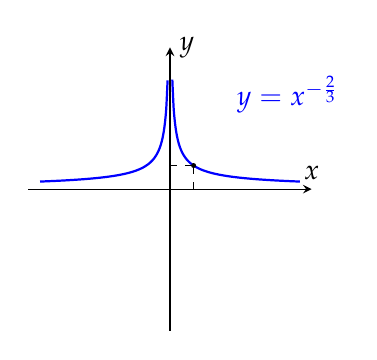
\begin{tikzpicture}[>=stealth,scale=0.3]
                        \draw[->] (-6,0) -- (6,0) node[above] {$x$};
                        \draw[->] (0,-6) -- (0,6) node[right] {$y$};
                        \draw[shift={(0,0)}] (0,0.1) -- (0,-0.1);
                        \draw[shift={(0,0)}] (0.1,0) -- (-0.1,0);
                        \draw[blue,smooth,thick,samples=100,domain=0.1:5.5] 
                            plot(\x,{\x^-0.6666}) node at (5,4){$y=x^{-\frac{2}{3}}$};
                        \draw[blue,smooth,thick,samples=100,domain=-5.5:-0.1] 
                            plot(\x,{-\x^-0.6666});
                        \fill (1,1) circle (3pt);
                        \draw[dashed] (1,1) -- (1,0);
                        \draw[dashed] (1,1) -- (0,1);
                    \end{tikzpicture}
                    \caption{函数$y=x^{-\frac{2}{3}}$}
                \end{minipage}
            }
        \end{center}
    \end{figure}
    \begin{figure}[h!]
        \begin{center}
            \subfigure
            {
                \begin{minipage}[t]{0.25\linewidth}
                    \begin{tikzpicture}[>=stealth,scale=0.3]
                        \draw[->] (-6,0) -- (6,0) node[above] {$x$};
                        \draw[->] (0,-6) -- (0,6) node[right] {$y$};
                        \draw[shift={(0,0)}] (0,0.1) -- (0,-0.1);
                        \draw[shift={(0,0)}] (0.1,0) -- (-0.1,0);
                        \draw[red,smooth,thick,samples=100,domain=-2.3:2.3] 
                            plot(\x,{\x*\x}) node at (5,4){$y=x^2$};
                        \fill (1,1) circle (3pt);
                        \draw[dashed] (1,1) -- (1,0);
                        \draw[dashed] (1,1) -- (0,1);
                    \end{tikzpicture}
                    \caption{函数$y=x^2$}
                \end{minipage}
            }\qquad\qquad\qquad
            \subfigure
            {
                \begin{minipage}[t]{0.25\linewidth}
                    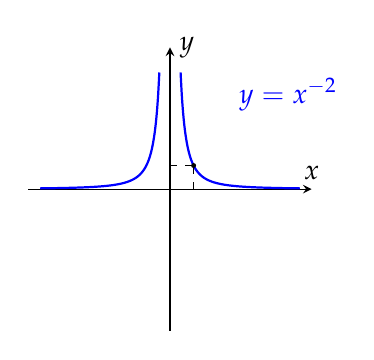
\begin{tikzpicture}[>=stealth,scale=0.3]
                        \draw[->] (-6,0) -- (6,0) node[above] {$x$};
                        \draw[->] (0,-6) -- (0,6) node[right] {$y$};
                        \draw[shift={(0,0)}] (0,0.1) -- (0,-0.1);
                        \draw[shift={(0,0)}] (0.1,0) -- (-0.1,0);
                        \draw[blue,smooth,thick,samples=100,domain=0.45:5.5] 
                            plot(\x,{\x^-2}) node at (5,4){$y=x^{-2}$};
                        \draw[blue,smooth,thick,samples=100,domain=-5.5:-0.45] 
                            plot(\x,{-\x^-2});
                        \fill (1,1) circle (3pt);
                        \draw[dashed] (1,1) -- (1,0);
                        \draw[dashed] (1,1) -- (0,1);
                    \end{tikzpicture}
                    \caption{函数$y=x^{-2}$}
                \end{minipage}
            }
        \end{center}
    \end{figure}
    \begin{figure}[h!]
        \begin{center}
            \subfigure
            {
                \begin{minipage}[t]{0.25\linewidth}
                    \begin{tikzpicture}[>=stealth,scale=0.3]
                        \draw[->] (-6,0) -- (6,0) node[above] {$x$};
                        \draw[->] (0,-6) -- (0,6) node[right] {$y$};
                        \draw[shift={(0,0)}] (0,0.1) -- (0,-0.1);
                        \draw[shift={(0,0)}] (0.1,0) -- (-0.1,0);
                        \draw[red,smooth,thick,samples=100,domain=-1.5:1.5] 
                            plot(\x,{\x*\x*\x*\x}) node at (5,4){$y=x^4$};
                        \fill (1,1) circle (3pt);
                        \draw[dashed] (1,1) -- (1,0);
                        \draw[dashed] (1,1) -- (0,1);
                    \end{tikzpicture}
                    \caption{函数$y=x^4$}
                \end{minipage}
            }\qquad\qquad\qquad
            \subfigure
            {
                \begin{minipage}[t]{0.25\linewidth}
                    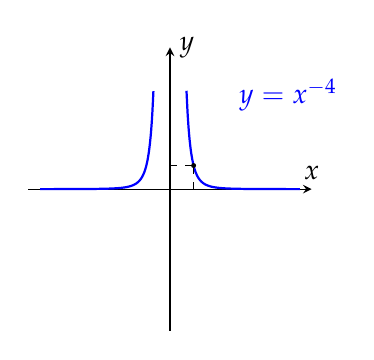
\begin{tikzpicture}[>=stealth,scale=0.3]
                        \draw[->] (-6,0) -- (6,0) node[above] {$x$};
                        \draw[->] (0,-6) -- (0,6) node[right] {$y$};
                        \draw[shift={(0,0)}] (0,0.1) -- (0,-0.1);
                        \draw[shift={(0,0)}] (0.1,0) -- (-0.1,0);
                        \draw[blue,smooth,thick,samples=100,domain=0.7:5.5] 
                            plot(\x,{\x^-4}) node at (5,4){$y=x^{-4}$};
                        \draw[blue,smooth,thick,samples=100,domain=-5.5:-0.7] 
                            plot(\x,{-\x^-4});
                        \fill (1,1) circle (3pt);
                        \draw[dashed] (1,1) -- (1,0);
                        \draw[dashed] (1,1) -- (0,1);
                    \end{tikzpicture}
                    \caption{函数$y=x^{-4}$}
                \end{minipage}
            }
        \end{center}
    \end{figure}

\newpage

    函数图像($n<0$~~~~~~$q$为奇数~~$p$为奇数):\vspace{5pt}
    \begin{figure}[h!]
        \begin{center}
            \subfigure
            {
                \begin{minipage}[t]{0.25\linewidth}
                    \begin{tikzpicture}[>=stealth,scale=0.3]
                        \draw[->] (-6,0) -- (6,0) node[above] {$x$};
                        \draw[->] (0,-6) -- (0,6) node[right] {$y$};
                        \draw[shift={(0,0)}] (0,0.1) -- (0,-0.1);
                        \draw[shift={(0,0)}] (0.1,0) -- (-0.1,0);
                        \draw[red,smooth,thick,samples=100,domain=-6:6] 
                            plot(\x,{\x^0.3333}) node at (5,4){$y=x^\frac{1}{3}$};
                        \fill (1,1) circle (3pt);
                        \draw[dashed] (1,1) -- (1,0);
                        \draw[dashed] (1,1) -- (0,1);
                    \end{tikzpicture}
                    \caption{函数$y=x^{\frac{1}{3}}$}
                \end{minipage}
            }\qquad\qquad\qquad
            \subfigure
            {
                \begin{minipage}[t]{0.25\linewidth}
                    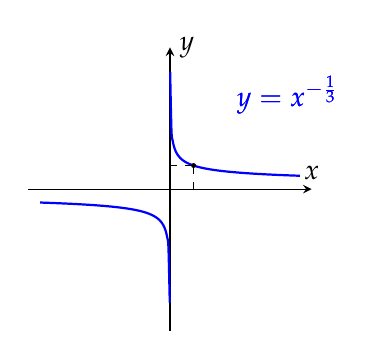
\begin{tikzpicture}[>=stealth,scale=0.3]
                        \draw[->] (-6,0) -- (6,0) node[above] {$x$};
                        \draw[->] (0,-6) -- (0,6) node[right] {$y$};
                        \draw[shift={(0,0)}] (0,0.1) -- (0,-0.1);
                        \draw[shift={(0,0)}] (0.1,0) -- (-0.1,0);
                        \draw[blue,smooth,thick,samples=100,domain=0.008:5.5] 
                            plot(\x,{\x^-0.3333}) node at (5,4){$y=x^{-\frac{1}{3}}$};
                        \draw[blue,smooth,thick,samples=100,domain=-5.5:-0.008] 
                            plot(\x,{\x^-0.3333}) node at (5,4){$y=x^{-\frac{1}{3}}$};
                        \fill (1,1) circle (3pt);
                        \draw[dashed] (1,1) -- (1,0);
                        \draw[dashed] (1,1) -- (0,1);
                    \end{tikzpicture}
                    \caption{函数$y=x^{-\frac{2}{3}}$}
                \end{minipage}
            }
        \end{center}
    \end{figure}
    \begin{figure}[h!]
        \begin{center}
            \subfigure
            {
                \begin{minipage}[t]{0.25\linewidth}
                    \begin{tikzpicture}[>=stealth,scale=0.3]
                        \draw[->] (-6,0) -- (6,0) node[above] {$x$};
                        \draw[->] (0,-6) -- (0,6) node[right] {$y$};
                        \draw[shift={(0,0)}] (0,0.1) -- (0,-0.1);
                        \draw[shift={(0,0)}] (0.1,0) -- (-0.1,0);
                        \draw[red,smooth,thick,samples=100,domain=-4.5:4.5] 
                            plot(\x,{\x}) node at (5,2.5){$y=x^1$};
                        \fill (1,1) circle (3pt);
                        \draw[dashed] (1,1) -- (1,0);
                        \draw[dashed] (1,1) -- (0,1);
                    \end{tikzpicture}
                    \caption{函数$y=x^1$}
                \end{minipage}
            }\qquad\qquad\qquad
            \subfigure
            {
                \begin{minipage}[t]{0.25\linewidth}
                    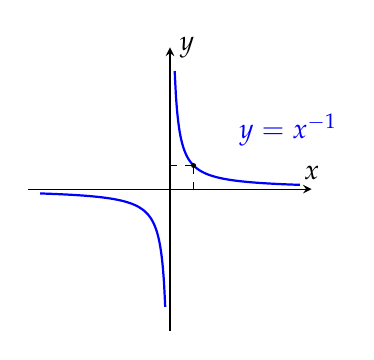
\begin{tikzpicture}[>=stealth,scale=0.3]
                        \draw[->] (-6,0) -- (6,0) node[above] {$x$};
                        \draw[->] (0,-6) -- (0,6) node[right] {$y$};
                        \draw[shift={(0,0)}] (0,0.1) -- (0,-0.1);
                        \draw[shift={(0,0)}] (0.1,0) -- (-0.1,0);
                        \draw[blue,smooth,thick,samples=100,domain=0.2:5.5] 
                            plot(\x,{\x^-1}) node at (5,2.5){$y=x^{-1}$};
                        \draw[blue,smooth,thick,samples=100,domain=-5.5:-0.2] 
                            plot(\x,{\x^-1});
                        \fill (1,1) circle (3pt);
                        \draw[dashed] (1,1) -- (1,0);
                        \draw[dashed] (1,1) -- (0,1);
                    \end{tikzpicture}
                    \caption{函数$y=x^{-1}$}
                \end{minipage}
            }
        \end{center}
    \end{figure}
    \begin{figure}[h!]
        \begin{center}
            \subfigure
            {
                \begin{minipage}[t]{0.25\linewidth}
                    \begin{tikzpicture}[>=stealth,scale=0.3]
                        \draw[->] (-6,0) -- (6,0) node[above] {$x$};
                        \draw[->] (0,-6) -- (0,6) node[right] {$y$};
                        \draw[shift={(0,0)}] (0,0.1) -- (0,-0.1);
                        \draw[shift={(0,0)}] (0.1,0) -- (-0.1,0);
                        \draw[red,smooth,thick,samples=100,domain=-1.73:1.73] 
                            plot(\x,{\x^3}) node at (5,4){$y=x^3$};
                        \fill (1,1) circle (3pt);
                        \draw[dashed] (1,1) -- (1,0);
                        \draw[dashed] (1,1) -- (0,1);
                    \end{tikzpicture}
                    \caption{函数$y=x^3$}
                \end{minipage}
            }\qquad\qquad\qquad
            \subfigure
            {
                \begin{minipage}[t]{0.25\linewidth}
                    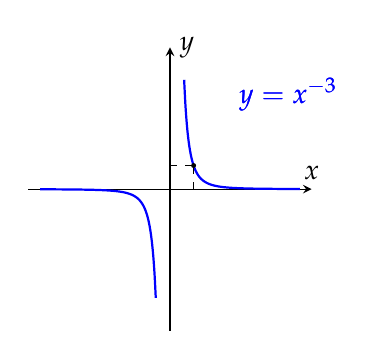
\begin{tikzpicture}[>=stealth,scale=0.3]
                        \draw[->] (-6,0) -- (6,0) node[above] {$x$};
                        \draw[->] (0,-6) -- (0,6) node[right] {$y$};
                        \draw[shift={(0,0)}] (0,0.1) -- (0,-0.1);
                        \draw[shift={(0,0)}] (0.1,0) -- (-0.1,0);
                        \draw[blue,smooth,thick,samples=100,domain=0.6:5.5] 
                            plot(\x,{\x^-3}) node at (5,4){$y=x^{-3}$};
                        \draw[blue,smooth,thick,samples=100,domain=-5.5:-0.6] 
                            plot(\x,{\x^-3}) node at (5,4){$y=x^{-3}$};
                        \fill (1,1) circle (3pt);
                        \draw[dashed] (1,1) -- (1,0);
                        \draw[dashed] (1,1) -- (0,1);
                    \end{tikzpicture}
                    \caption{函数$y=x^{-3}$}
                \end{minipage}
            }
        \end{center}
    \end{figure}

\newpage

\subsection{指数函数}
    我们将符合以下形式的函数称为指数函数:
    \begin{large}
        \begin{equation*}
            y=n^x\qquad n\in\mathbb{R^+}
        \end{equation*}
    \end{large}\\
    在指数函数中,自变量$x$是指数,参数$n$是底数。\\[3mm]
    指数函数的函数图像性质和参数$n$有关,具体可以分为两种:\vspace{5pt}
    \begin{table}[h]
        \begin{center}
            \begin{tabular}{l|l|l}
                \hline
                参数取值&示例&图像特征\\ \hline
                $n<1$\qquad\qquad&$y=\frac{1}{2}^x$\quad~~~$y=\frac{1}{3}^x$&单调递减函数\qquad\qquad\\ \hline
                $n>1$\qquad\qquad&$y=2^x$\qquad$y=3^x\qquad$&单调递减函数\\ \hline
            \end{tabular}
            \caption{指数函数的图像性质}
        \end{center}
    \end{table}\\
    指数函数无论参数如何变化,其图像必然过点$(0,1)$。\\[3mm]
    函数图像($n<1$):\vspace{-5pt}
    \begin{figure}[h!]
        \begin{center}
            \subfigure
            {
                \begin{minipage}[t]{0.25\linewidth}
                    \begin{tikzpicture}[>=stealth,scale=0.3]
                        \draw[->] (-6,0) -- (6,0) node[above] {$x$};
                        \draw[->] (0,-6) -- (0,6) node[right] {$y$};
                        \draw[shift={(0,0)}] (0,0.1) -- (0,-0.1);
                        \draw[shift={(0,0)}] (0.1,0) -- (-0.1,0);
                        \draw[red,smooth,thick,samples=100,domain=-2.32:5] 
                            plot(\x,{0.5^\x}) node at (5,4){$y=\dfrac{1}{2}^x$};
                        \fill (0,1) circle (3pt);
                    \end{tikzpicture}
                    \caption{函数$y=\dfrac{1}{2}^x$}
                \end{minipage}
            }\qquad\qquad\qquad
            \subfigure
            {
                \begin{minipage}[t]{0.25\linewidth}
                    \begin{tikzpicture}[>=stealth,scale=0.3]
                        \draw[->] (-6,0) -- (6,0) node[above] {$x$};
                        \draw[->] (0,-6) -- (0,6) node[right] {$y$};
                        \draw[shift={(0,0)}] (0,0.1) -- (0,-0.1);
                        \draw[shift={(0,0)}] (0.1,0) -- (-0.1,0);
                        \draw[blue,smooth,thick,samples=100,domain=-1.465:5] 
                            plot(\x,{0.3333^\x}) node at (5,4){$y=\dfrac{1}{3}^x$};
                        \fill (0,1) circle (3pt);
                    \end{tikzpicture}
                    \caption{函数$y=\dfrac{1}{3}^x$}
                \end{minipage}
            }
        \end{center}
    \end{figure}\\
    函数图像($n>1$):\vspace{-5pt}
    \begin{figure}[h!]
        \begin{center}
            \subfigure
            {
                \begin{minipage}[t]{0.25\linewidth}
                    \begin{tikzpicture}[>=stealth,scale=0.3]
                        \draw[->] (-6,0) -- (6,0) node[above] {$x$};
                        \draw[->] (0,-6) -- (0,6) node[right] {$y$};
                        \draw[shift={(0,0)}] (0,0.1) -- (0,-0.1);
                        \draw[shift={(0,0)}] (0.1,0) -- (-0.1,0);
                        \draw[red,smooth,thick,samples=100,domain=-5:2.32] 
                            plot(\x,{2^\x}) node at (5,4){$y=2^x$};
                        \fill (0,1) circle (3pt);
                    \end{tikzpicture}
                    \caption{函数$y=2^x$}
                \end{minipage}
            }\qquad\qquad\qquad
            \subfigure
            {
                \begin{minipage}[t]{0.25\linewidth}
                    \begin{tikzpicture}[>=stealth,scale=0.3]
                        \draw[->] (-6,0) -- (6,0) node[above] {$x$};
                        \draw[->] (0,-6) -- (0,6) node[right] {$y$};
                        \draw[shift={(0,0)}] (0,0.1) -- (0,-0.1);
                        \draw[shift={(0,0)}] (0.1,0) -- (-0.1,0);
                        \draw[blue,smooth,thick,samples=100,domain=-5:1.465] 
                            plot(\x,{3^\x}) node at (5,4){$y=3^x$};
                        \fill (0,1) circle (3pt);
                    \end{tikzpicture}
                    \caption{函数$y=3^x$}
                \end{minipage}
            }
        \end{center}
    \end{figure}

\newpage

\subsection{对数函数}
    我们将符合以下形式的函数称为对数函数:
    \begin{large}
        \begin{equation*}
            y=\log_{n}{x}\qquad x\in\mathbb{R^+}
        \end{equation*}
    \end{large}\\
    在对数函数中,自变量$x$是真数,参数$n$是底数。\\[3mm]
    对数函数的函数图像性质和参数$n$有关,具体可以分为两种:\vspace{5pt}
    \begin{table}[h]
        \begin{center}
            \begin{tabular}{l|l|l}
                \hline
                参数取值&示例&图像特征\\ \hline
                $n<1$\qquad\qquad&$y=\log_{\frac{1}{2}}x$\qquad$y=\log_{\frac{1}{3}}x$&单调递减函数\qquad\qquad\\ \hline
                $n>1$\qquad\qquad&$y=\log_{2}x$\qquad\,$y=\log_{3}x$\qquad\qquad&单调递增函数\\ \hline
            \end{tabular}
            \caption{对数函数的图形性质}
        \end{center}
    \end{table}\\
    对数函数无论参数如何变化,其图像必然过点$(1,0)$。\\[3mm]
    函数图像($n<1$):\vspace{-5pt}
    \begin{figure}[h!]
        \begin{center}
            \subfigure
            {
                \begin{minipage}[t]{0.25\linewidth}
                    \begin{tikzpicture}[>=stealth,scale=0.3]
                        \draw[->] (-6,0) -- (6,0) node[above] {$x$};
                        \draw[->] (0,-6) -- (0,6) node[right] {$y$};
                        \draw[shift={(0,0)}] (0,0.1) -- (0,-0.1);
                        \draw[shift={(0,0)}] (0.1,0) -- (-0.1,0);
                        \draw[red,smooth,thick,samples=100,domain=0.05:6] 
                            plot(\x,{-log10(\x)/0.301}) node at (5,4){$y=\log_{\frac{1}{2}}x$};
                        \fill (1,0) circle (3pt);
                    \end{tikzpicture}
                    \caption{函数$y=\log_{\frac{1}{2}}x$}
                \end{minipage}
            }\qquad\qquad\qquad
            \subfigure
            {
                \begin{minipage}[t]{0.25\linewidth}
                    \begin{tikzpicture}[>=stealth,scale=0.3]
                        \draw[->] (-6,0) -- (6,0) node[above] {$x$};
                        \draw[->] (0,-6) -- (0,6) node[right] {$y$};
                        \draw[shift={(0,0)}] (0,0.1) -- (0,-0.1);
                        \draw[shift={(0,0)}] (0.1,0) -- (-0.1,0);
                        \draw[blue,smooth,thick,samples=100,domain=0.02:6] 
                            plot(\x,{-log10(\x)/0.477}) node at (5,4){$y=\log_{\frac{1}{3}}x$};
                        \fill (1,0) circle (3pt);
                    \end{tikzpicture}
                    \caption{函数$y=\log_{\frac{1}{3}}x$}
                \end{minipage}
            }
        \end{center}
    \end{figure}\\
    函数图像($n>1$):\vspace{-5pt}
    \begin{figure}[h!]
        \begin{center}
            \subfigure
            {
                \begin{minipage}[t]{0.25\linewidth}
                    \begin{tikzpicture}[>=stealth,scale=0.3]
                        \draw[->] (-6,0) -- (6,0) node[above] {$x$};
                        \draw[->] (0,-6) -- (0,6) node[right] {$y$};
                        \draw[shift={(0,0)}] (0,0.1) -- (0,-0.1);
                        \draw[shift={(0,0)}] (0.1,0) -- (-0.1,0);
                        \draw[red,smooth,thick,samples=100,domain=0.05:6] 
                            plot(\x,{log10(\x)/0.301}) node at (5,4){$y=\log_{2}x$};
                        \fill (1,0) circle (3pt);
                    \end{tikzpicture}
                    \caption{函数$y=\log_{2}x$}
                \end{minipage}
            }\qquad\qquad\qquad
            \subfigure
            {
                \begin{minipage}[t]{0.25\linewidth}
                    \begin{tikzpicture}[>=stealth,scale=0.3]
                        \draw[->] (-6,0) -- (6,0) node[above] {$x$};
                        \draw[->] (0,-6) -- (0,6) node[right] {$y$};
                        \draw[shift={(0,0)}] (0,0.1) -- (0,-0.1);
                        \draw[shift={(0,0)}] (0.1,0) -- (-0.1,0);
                        \draw[blue,smooth,thick,samples=100,domain=0.02:6] 
                            plot(\x,{log10(\x)/0.477}) node at (5,4){$y=\log_{3}x$};
                        \fill (1,0) circle (3pt);
                    \end{tikzpicture}
                    \caption{函数$y=\log_{3}x$}
                \end{minipage}
            }
        \end{center}
    \end{figure}

\newpage

\section{三角比的运算}

\subsection{角度}
    角度制是衡量角的大小的一种方式,单位是度。\\[3mm]
    我们定义$1$度为周角的$360$等分。\\[3mm]
    按逆时针方向旋转所形成的角称为正角,其度量值为正。\\[3mm]
    按顺时针方向旋转所形成的角称为负角,其度量值为负。\\[3mm]
    根据角度定义,在角度制中,周角的大小是$360$度。\\[3mm]
    在研究三角函数时,我们通常会默认角的顶点位于坐标原点,
    角的始边与$x$轴正半轴重合。

\subsection{弧度}
    弧度制是衡量角的大小的一种方式,单位是弧度。\\[3mm]
    我们定义$1$弧度为单位圆上弧长为一的弧所对应的圆心角的大小。\\[3mm]
    弧度的意义在于填补了角度制的设计缺陷,大幅度简化了运算。\\[3mm]
    弧度在使用中,可以省略弧度单位,直接书写弧度数即可。\\[3mm]
    根据弧度定义,在弧度制中,周角的大小是$2\pi$弧度。

\subsection{扇形的弧长和面积}
    弧度的本质是单位圆上的角所对应的弧长,
    所以考虑圆的半径,我们就可以得出:\\[3mm]
    扇形的弧长公式:
    \begin{large}
        \begin{equation*}
            l=\alpha \cdot r    
        \end{equation*}   
    \end{large}\\
    我们知道圆的面积可以用$\pi r^2$计算,
    显然扇形的面积和圆的面积比可以使用$\dfrac{\alpha}{2\pi}$表示。\\[3mm]
    因此我们可以通过将两者相乘,得到关于弧度和半径的扇形面积公式。\\[3mm]
    同时我们可以再代入弧长公式,得到关于弧长和半径的扇形面积公式。\\[3mm]
    扇形的面积公式:
    \begin{large}
        \begin{align*}
            &S=\frac{1}{2}\cdot \alpha \cdot r^2=\frac{1}{2}\cdot l \cdot r
        \end{align*}
    \end{large}

\newpage

\subsection{三角比的定义}
    设三角形终边上一点$P(x,y)$,
    同时令原点到点P的距离$OP=r$,其中$r=\sqrt{x^2+y^2}$。\\[5mm]
    首先定义以下三角比:\\[3mm]
    正弦($\sin$):
    \begin{large}
    \begin{equation*}
        \sin{\alpha}=\dfrac{y}{r}
    \end{equation*}   
    \end{large}\\
    余弦($\cos$):
    \begin{large}
    \begin{equation*}
        \cos{\alpha}=\dfrac{x}{r}
    \end{equation*}   
    \end{large}\\
    正切($\tan$):
    \begin{large}
    \begin{equation*}
        \tan{\alpha}=\dfrac{y}{x}
    \end{equation*}   
    \end{large}\\
    然后定义以下三角比:\\[3mm]
    余割($\csc$):
    \begin{large}
    \begin{equation*}
        \csc{\alpha}=\dfrac{r}{y}
    \end{equation*}   
    \end{large}\\
    正割($\sec$):
    \begin{large}
    \begin{equation*}
        \sec{\alpha}=\dfrac{r}{x}
    \end{equation*}   
    \end{large}\\
    余切($\cot$):
    \begin{large}
    \begin{equation*}
        \cot{\alpha}=\dfrac{x}{y}
    \end{equation*}   
    \end{large}\\[3mm]
    特别的,如果在一个单位圆上,角$\alpha$的终边与单位圆的交点为P$(x,y)$,直线$OP$的斜率为$k$。\\[3mm]
    那么存在以下关系:
    \begin{large}
        \begin{align*}
            &x=\cos{\alpha}\\[3mm]
            &y=\sin{\alpha}\\[3mm]
            &k=\tan{\alpha}
        \end{align*}
    \end{large}

\newpage

\subsection{同角三角比的关系}
    由于$\sin$和$\csc$互为倒数,$\cos$和$\sec$互为倒数,$\tan$和$\cot$互为倒数,我们可以得到倒数关系。\\[3mm]
    \textbf{倒数关系:}
    \begin{large}
        \begin{equation*}
            \sin{\alpha} \cdot \csc{\alpha}=1
        \end{equation*}
        \begin{equation*}
            \cos{\alpha} \cdot \sec{\alpha}=1
        \end{equation*}   
        \begin{equation*}
            \tan{\alpha} \cdot \cot{\alpha}=1
        \end{equation*}
    \end{large}\\
    由于$\sin \alpha=\dfrac{y}{r}$,同时$\cos \alpha=\dfrac{x}{r}$,且$\tan \alpha=\dfrac{y}{x}$,通过两者相除可以得到商数关系。\\[3mm]
    \textbf{商数关系:}
    \begin{large}
        \begin{equation*}
            \tan \alpha=\frac{\sin \alpha}{\cos \alpha}
        \end{equation*}
    \end{large}\\[4mm]
    通过以下推导,我们可以得出平方关系:\vspace{5pt}
    \setcounter{equation}{0}
    \begin{equation}
        \sin^2{\alpha}+\cos^2{\alpha}
        =\frac{y^2}{r^2}+\frac{x^2}{r^2}
        =\frac{x^2+y^2}{r^2}
        =\frac{x^2+y^2}{x^2+y^2}
        =1
    \end{equation}\vspace{5pt}
    \begin{equation}
        \sec^2 \alpha-\tan^2 \alpha
        =\frac{r^2}{x^2}-\frac{y^2}{x^2}
        =\frac{x^2+y^2}{x^2}-\frac{y^2}{x^2}
        =1
    \end{equation}\vspace{5pt}
    \begin{equation}
        \csc^2 \alpha-\cot^2 \alpha
        =\frac{r^2}{y^2}-\frac{x^2}{y^2}
        =\frac{x^2+y^2}{y^2}-\frac{x^2}{y^2}
        =1
    \end{equation}\\
    \textbf{平方关系:}
    \begin{large}
        \begin{equation*}
            \sin^2 \alpha +\cos^2 \alpha=1
        \end{equation*}
        \begin{equation*}
            \sec^2 \alpha -\tan^2 \alpha=1
        \end{equation*}
        \begin{equation*}
            \csc^2 \alpha -\cot^2 \alpha=1
        \end{equation*}
    \end{large}

\newpage

\subsection{第一组诱导公式}
    第一组诱导公式讨论了$\alpha$和$2\pi+\alpha$的关系。\\[3mm]
    我们知道,两个相差$2\pi$的角的终边是相同的,所以我们可以得到:\\
    \newline
    \textbf{第一组诱导公式:}
    \begin{large}
    \begin{align*}
        &\sin{(2\pi+\alpha)}=\sin{\alpha}\\[3mm]
        &\cos{(2\pi+\alpha)}=\cos{\alpha}\\[3mm]
        &\tan{(2\pi+\alpha)}=\tan{\alpha}
    \end{align*}
    \end{large}

\subsection{第二组诱导公式}
    第二组诱导公式讨论了$\alpha$和$-\alpha$的关系\\[3mm]
    角$\alpha$与单位圆的交点为:$P(\cos{\alpha},\sin{\alpha})$\\
    角$-\alpha$与单位圆的交点为:$P^{'}(\cos{(-\alpha)},\sin{(-\alpha)})$\\[3mm]
    显然点$P$和点$P^{'}$关于x轴对称,
    所以点$P^{'}$也可以写为$(\cos{\alpha},-\sin{\alpha})$。\\[3mm]
    对于正切,我们可以通过三角比的商数关系求得。\\
    \newline
    \textbf{第二组诱导公式:}
    \begin{large}
    \begin{align*}
        &\sin{(-\alpha)}=-\sin{\alpha}\\[3mm]
        &\cos{(-\alpha)}=\cos{\alpha}\\[3mm]
        &\tan{(-\alpha)}=-\tan{\alpha}
    \end{align*}
    \end{large}

\newpage

\subsection{第三组诱导公式}
    第三组诱导公式讨论了$\alpha$和$\alpha+\pi$的关系。\\[3mm]
    角$\alpha$与单位圆的交点为:$P(\cos{\alpha},\sin{\alpha})$\\
    角$\pi+\alpha$与单位圆的交点为:$P^{'}(\cos{(\pi+\alpha)},\sin{(\pi+\alpha)})$\\[3mm]
    由于两个角相差$180$度,点$P$和点$P^{'}$关于原点对称,
    所以点$P^{'}$也可也写为$(-\cos{\alpha},-\sin{\alpha})$。\\[3mm]
    对于正切,我们仍然可以通过三角比的商数关系求得。\\
    \newline
    \textbf{第三组诱导公式:}
    \begin{large}
    \begin{align*}
        &\sin{(\pi+\alpha)}=-\sin \alpha\\[3mm]
        &\cos{(\pi+\alpha)}=-\cos \alpha\\[3mm]
        &\tan{(\pi+\alpha)}=\tan \alpha
    \end{align*}
    \end{large}

\subsection{第四组诱导公式}
    第四组诱导公式讨论了$\alpha$和$\pi-\alpha$的关系。\\[3mm]
    角$\alpha$与单位圆的交点为:$P(\cos{\alpha},\sin{\alpha})$\\
    角$\pi-\alpha$与单位圆的交点为:$P^{'}(\cos{(\pi-\alpha)},\sin{(\pi-\alpha)})$\\[3mm]
    我们可以这样理解,首先将$\alpha$变换为$-\alpha$,
    也就是先关于$x$轴对称,接下来再将$-\alpha$变换为$\pi-\alpha$,
    即再关于原点对称,总体来看便是关于$y$轴对称,
    所以点$P^{'}$也可也写为$(-\cos{\alpha},\sin{\alpha})$。\\[3mm]
    对于正切,我们依然可以通过三角比的商数关系求得。\\
    \newline
    \textbf{第四组诱导公式:}
    \begin{large}
    \begin{align*}
        &\sin{(\pi-\alpha)}=\sin \alpha\\[3mm]
        &\cos{(\pi-\alpha)}=-\cos \alpha\\[3mm]
        &\tan{(\pi-\alpha)}=-\tan \alpha
    \end{align*}
    \end{large}

\newpage

\subsection{诱导公式和角度的图形变换}
    综合考虑前四个诱导公式,
    我们会发现其本质都是对于角度的图形变换:
    \begin{table}[h]
        \begin{center}
            \begin{tabular}{l|l|l|l|l|l}
                \hline
                变换方式~~~~~~~~&诱导公式~~~~~~~~&参数~~~~~~&sin[x]~~~~&cos[y]~~~~&tan[k]~~~~\\ \hline
                不变换&第一组诱导公式&$+\ \alpha$&$+$&$+$&$+$\\ \hline
                关于$x$轴对称&第二组诱导公式&$-\ \alpha$&$-$&$+$&$-$\\ \hline
                关于$y$轴对称&第四组诱导公式&$-\ \alpha+\pi$&$+$&$-$&$-$\\ \hline
                关于原点对称&第三组诱导公式&$+\ \alpha+\pi$&$-$&$-$&$+$\\ \hline
            \end{tabular}        
            \caption{诱导公式和角度的图形变换}
        \end{center}
    \end{table}\vspace{-10pt}

\subsection{余弦的和差公式}
    设$\alpha$和$\beta$两个任意角,
    两角终边与单位圆的交点为$A(\cos \alpha,\sin \alpha)$和$B(\cos \beta,\sin \beta)$。\\[3mm]
    接下来将$OA$和$OB$绕$O$旋转$-\beta$,
    使得点$A^{'}(\cos{(\alpha-\beta)},\sin{(\alpha-\beta)})$,点$B^{'}(1,0)$。\\[3mm]
    根据两点之间距离公式:
    \setcounter{equation}{0}
    \begin{align}
        |AB|^2
        &=(\cos \alpha-\cos \beta)^2+(\sin \alpha- \sin \beta)^2\\
        &=\cos^2{\alpha}+\cos^2{\beta}-2 \cdot \cos{\alpha} \cdot \cos{\beta}+\sin^2{\alpha}+\sin^2{\beta}-2 \cdot \sin{\alpha} \cdot \sin{\beta}\\
        &=2-2 \cdot \cos{\alpha} \cdot \cos{\beta}-2 \cdot \sin{\alpha} \cdot \sin{\beta}\\
        &=2-2 \cdot \left(\cos{\alpha}\cdot\cos{\beta}+\sin{\alpha}\cdot\sin{\beta}\right)\\[6mm]
        |A^{'}B^{'}|^2
        &=\left(\cos{(\alpha-\beta)}-1\right)^2+\left(\sin{(\alpha-\beta)}\right)^2\\
        &=\cos^2{(\alpha-\beta)}-2\cdot\cos{\alpha-\beta}+1+\sin^2{(\alpha-\beta)}\\
        &=2-2\cdot\cos{(\alpha-\beta)}
    \end{align}\\
    由于$|AB|=|A^{'}B^{'}|$,
    所以有$2-2 \cdot \left(\cos{\alpha}\cdot\cos{\beta}+\sin{\alpha}\cdot\sin{\beta}\right)=2-2\cdot\cos{(\alpha-\beta)}$,化简可得:\\[3mm]
    \textbf{两角差的余弦公式:}
    \begin{large}
    \begin{equation*}
        \cos{(\alpha-\beta)}=\cos{\alpha}\cdot\cos{\beta}+\sin{\alpha}\cdot\sin{\beta}
    \end{equation*}
    \end{large}\\[4mm]
    在两角差的余弦公式中,用$-\beta$替代$\beta$,那么我们可以得到:\\[3mm]
    \textbf{两角和的余弦公式:}
    \begin{large}
    \begin{equation*}
        \cos{(\alpha+\beta)}=\cos{\alpha}\cdot\cos{\beta}-\sin{\alpha}\cdot\sin{\beta}
    \end{equation*}
    \end{large}

\newpage

\subsection{第五组诱导公式}
    第五组诱导公式讨论了$\alpha$和$\dfrac{\pi}{2}-\alpha$的关系。\\
    \setcounter{equation}{0}
    \begin{align}
        \cos{\left(\dfrac{\pi}{2}-\alpha\right)}
        &=\cos{\frac{\pi}{2}}\cdot\cos{\alpha}+\sin{\frac{\pi}{2}}\cdot\sin{\alpha}\qquad\qquad\qquad\qquad\\[3mm]
        &=0\cdot\cos{\alpha}+1\cdot\sin{\alpha}\\[3mm]
        &=\sin{\alpha}\\[6mm]
        \sin{\left(\frac{\pi}{2}-\alpha\right)}
        &=\cos{\left(\frac{\pi}{2}-\left(\frac{\pi}{2}-\alpha\right)\right)}\\[3mm]
        &=\cos{\left(\frac{\pi}{2}-\frac{\pi}{2}+\alpha\right)}\\[3mm]
        &=\cos{(\alpha)}\\[6mm]
        \tan{\left(\frac{\pi}{2}-\alpha\right)}
        &=\frac{\sin{\left(\dfrac{\pi}{2}-\alpha\right)}}{\cos{\left(\dfrac{\pi}{2}-\alpha\right)}}=\frac{\cos{\alpha}}{\sin{\alpha}}=\cot{\alpha}\\[6mm]
        \cot{\left(\frac{\pi}{2}-\alpha\right)}
        &=\frac{\cos{\left(\dfrac{\pi}{2}-\alpha\right)}}{\sin{\left(\dfrac{\pi}{2}-\alpha\right)}}=\frac{\sin{\alpha}}{\cos{\alpha}}=\tan{\alpha}
    \end{align}\\[3mm]
    \textbf{第五组诱导公式:}
    \begin{large}
    \begin{align*}
        &\sin{\left(\frac{\pi}{2}-\alpha\right)}=\cos{\alpha}\\[4mm]
        &\cos{\left(\frac{\pi}{2}-\alpha\right)}=\sin{\alpha}\\[4mm]
        &\tan{\left(\frac{\pi}{2}-\alpha\right)}=\cot{\alpha}\\[4mm]
        &\cot{\left(\frac{\pi}{2}-\alpha\right)}=\tan{\alpha}
    \end{align*}
    \end{large}

\newpage

\subsection{第六组诱导公式}
    第六组诱导公式讨论了$\alpha$和$\dfrac{\pi}{2}+\alpha$的关系。\\[4mm]
    使用$\alpha$替换第五组诱导公式:
    \setcounter{equation}{0}
    \begin{align}
        &\sin{\left(\frac{\pi}{2}+\alpha\right)}=\sin{\frac{\pi}{2}+\left(-(-\alpha)\right)}=\cos{(-\alpha)}=\cos{\alpha}\\[3mm]
        &\cos{\left(\frac{\pi}{2}+\alpha\right)}=\cos{\frac{\pi}{2}+\left(-(-\alpha)\right)}=\sin{(-\alpha)}=-\sin{\alpha}\\[3mm]
        &\tan{\left(\frac{\pi}{2}+\alpha\right)}=\tan{\frac{\pi}{2}+\left(-(-\alpha)\right)}=\cot{(-\alpha)}=-\cot{\alpha}\\[3mm]
        &\cot{\left(\frac{\pi}{2}+\alpha\right)}=\cot{\frac{\pi}{2}+\left(-(-\alpha)\right)}=\tan{(-\alpha)}=-\tan{\alpha}
    \end{align}\\[3mm]
    \textbf{第六组诱导公式:}
    \begin{large}
    \begin{align*}
        &\sin{\left(\frac{\pi}{2}+\alpha\right)}=\cos{\alpha}\\[4mm]
        &\cos{\left(\frac{\pi}{2}+\alpha\right)}=-\sin{\alpha}\\[4mm]
        &\tan{\left(\frac{\pi}{2}+\alpha\right)}=-\cot{\alpha}\\[4mm]
        &\cot{\left(\frac{\pi}{2}+\alpha\right)}=-\tan{\alpha}
    \end{align*}        
    \end{large}

\newpage

\subsection{正弦的和差公式}
    通过余弦的和差公式和第五组诱导公式,我们就可以推导正弦的和差公式:\\
    \setcounter{equation}{0}
    \begin{align}
        \sin{(\alpha+\beta)}
        &=\cos{\left(\frac{\pi}{2}-(\alpha+\beta)\right)}\qquad\qquad\qquad\qquad\\[3mm]
        &=\cos{\left(\left(\frac{\pi}{2}-\alpha\right)-\beta\right)}\\[3mm]
        &=\cos{(\frac{\pi}{2}-\alpha)}\cdot\cos{\beta}+\sin{(\frac{\pi}{2}-\alpha)}\cdot\sin{\beta}\\[3mm]
        &=\sin{\alpha}\cdot\cos{\beta}+\cos{\alpha}\cdot\sin{\beta}
    \end{align}
    \textbf{两角和的正弦公式:}
    \begin{large}
    \begin{equation*}
        \sin{(\alpha+\beta)}=\sin{\alpha}\cdot\cos{\beta}+\cos{\alpha}\cdot\sin{\beta}
    \end{equation*}\\        
    \end{large}
    在两角和的正弦公式中,用$\beta$替换$-\beta$,可以得到:\\
    \newline
    \textbf{两角差的余弦公式:}
    \begin{large}
    \begin{equation*}
        \sin{(\alpha-\beta)}=\sin{\alpha}\cdot\cos{\beta}-\cos{\alpha}\cdot\sin{\beta}
    \end{equation*}      
    \end{large}

\subsection{正切的和差公式}
    由于已经推导出了正弦和余弦的和差公式,
    通过商数关系,我们可以推出正切的和差公式:\\
    \setcounter{equation}{0}
    \begin{align}
        &\tan{(\alpha+\beta)}
        =\frac{\sin{(\alpha+\beta)}}{\cos{(\alpha+\beta)}}
        =\frac{\sin{\alpha}\cdot\cos{\beta}+\cos{\alpha}\cdot\sin{\beta}}{\cos{\alpha}\cdot\cos{\beta}-\sin{\alpha}\cdot\sin{\beta}}
        =\frac{\tan{\alpha}\cdot1+1\cdot\tan{\beta}}{1-\tan{\alpha}\cdot\tan{\beta}}\\[4mm]
        &\tan{(\alpha-\beta)}
        =\frac{\sin{(\alpha-\beta)}}{\cos{(\alpha-\beta)}}
        =\frac{\sin{\alpha}\cdot\cos{\beta}-\cos{\alpha}\cdot\sin{\beta}}{\cos{\alpha}\cdot\cos{\beta}+\sin{\alpha}\cdot\sin{\beta}}
        =\frac{\tan{\alpha}\cdot1-1\cdot\tan{\beta}}{1+\tan{\alpha}\cdot\tan{\beta}}
    \end{align}\\
    \textbf{两角和的正切公式}
    \begin{large}
        \begin{equation*}
            \tan{(\alpha+\beta)}=\frac{\tan{\alpha}+\tan{\beta}}{1-\tan{\alpha}\cdot\tan{\beta}}
        \end{equation*}\\
    \end{large}
    \textbf{两角差的正切公式}
    \begin{large}
        \begin{equation*}
            \tan{(\alpha-\beta)}=\frac{\tan{\alpha}-\tan{\beta}}{1+\tan{\alpha}\cdot\tan{\beta}}
        \end{equation*} 
    \end{large}

\newpage

\subsection{辅助角公式}
    \textbf{辅助角公式:}
    \begin{large}
    \begin{equation*}
        a\cdot\sin{\alpha}+b\cdot\cos{\alpha}=\sqrt{a^2+b^2}\cdot\sin{(\alpha+\beta)}\qquad\cos{\beta}=\frac{a}{\sqrt{a^2+b^2}}\qquad\sin{\beta}=\frac{b}{\sqrt{a^2+b^2}}
    \end{equation*}        
    \end{large}\\
    推导如下:
    \setcounter{equation}{0}
    \begin{align}
        a\cdot\sin{\alpha}+b\cdot\cos{\alpha}
        &=\sqrt{a^2+b^2}\cdot\left(\frac{a}{\sqrt{a^2+b^2}}\cdot\sin{\alpha}+\frac{b}{\sqrt{a^2+b^2}}\cdot\cos{\alpha}\right)\\[3mm] 
        &=\sqrt{a^2+b^2}\cdot\left(\sin{\alpha}\cdot\cos{\beta}+\cos{\alpha}\cdot\sin{\beta}\right)\\[3mm]
        &=\sqrt{a^2+b^2}\cdot\sin{(\alpha+\beta)}
    \end{align}

\subsection{倍角的三角比}
    对于三角比的和公式,特别的,当$\alpha=\beta$时,我们可以有:
    \begin{align}
        &\sin{(\alpha+\alpha)}=\sin{\alpha}\cdot\cos{\alpha}+\cos{\alpha}\cdot\sin{\alpha}\\[3mm]
        &\cos{(\alpha+\alpha)}=\cos{\alpha}\cdot\cos{\alpha}-\sin{\alpha}\cdot\sin{\alpha}\\[3mm]
        &\tan{(\alpha+\alpha)}=\frac{\tan{\alpha}+\tan{\alpha}}{1-\tan{\alpha}\cdot\tan{\alpha}}
    \end{align}\\
    \textbf{正弦的倍角公式:}
    \begin{large}
    \begin{equation*}
        \sin{2\alpha}=2\cdot\sin{\alpha}\cdot\cos{\alpha}
    \end{equation*}
    \end{large}\\
    对于$\cos{2\alpha}$,可以再结合公式$\sin^2{\alpha}+\cos^2{\alpha}=1$,
    得出另外两种表达形式。\\[3mm]
    \textbf{余弦的倍角公式:}
    \begin{large}
    \begin{align*}
        &\cos{2\alpha}=\cos^2{\alpha}-\sin^2{\alpha}\\[3mm]
        &\cos{2\alpha}=2\cdot\cos^2{\alpha}-1\\[3mm]
        &\cos{2\alpha}=1-2\cdot\sin^2{\alpha}
    \end{align*}
    \end{large}\\
    \textbf{正切的倍角公式:}
    \begin{large}
    \begin{equation*}
        \tan{2\alpha}=\frac{2\cdot\tan{\alpha}}{1-\tan^2{\alpha}}
    \end{equation*}
    \end{large}
    
\newpage

\subsection{半角的三角比}
    将余弦的倍角公式中使用$\beta$替代$2\alpha$:\\
    \setcounter{equation}{0}
    \begin{align}
        &\cos{2\alpha}=2\cdot\cos^2{\alpha}-1\\[3mm]
        &\cos{\beta}=2\cdot\cos^2{\frac{\beta}{2}}-1\\[3mm]
        &2\cdot\cos^2{\frac{\beta}{2}}=1+\cos{\beta}\\[3mm]
        &\cos^2{\frac{\beta}{2}}=\frac{1+\cos{\beta}}{2}\\[3mm]
        &\cos{\frac{\beta}{2}}=\pm\sqrt{\frac{1+\cos{\beta}}{2}}\\[8mm]
        &\cos{2\alpha}=1-2\cdot\sin^2{\alpha}\\[3mm]
        &\cos{\beta}=1-2\cdot\sin^2{\frac{\beta}{2}}\\[3mm]
        &2\cdot\sin^2{\frac{\beta}{2}}=1-\cos{\beta}\\[3mm]
        &\sin^2{\frac{\beta}{2}}=\frac{1-\cos{\beta}}{2}\\[3mm]
        &\sin{\frac{\beta}{2}}=\pm\sqrt{\frac{1-\cos{\beta}}{2}}
    \end{align}\\
    \newline
    \textbf{正弦的半角公式:}
    \begin{large}
    \begin{equation*}
        \sin{\frac{\beta}{2}}=\pm\sqrt{\frac{1-\cos{\beta}}{2}}
    \end{equation*}        
    \end{large}\\
    \textbf{余弦的半角公式:}
    \begin{large}
    \begin{equation*}
        \cos{\frac{\beta}{2}}=\pm\sqrt{\frac{1+\cos{\beta}}{2}}
    \end{equation*}
    \end{large}

\newpage
    通过商数关系可以推导正切的半角公式:\\
    \begin{align}
        \tan{\frac{\beta}{2}}&=\frac{\pm\sqrt{\dfrac{1-\cos{\beta}}{2}}}{\pm\sqrt{\dfrac{1+\cos{\beta}}{2}}}
        =\pm\sqrt{\frac{1-\cos{\beta}}{1+\cos{\beta}}}
    \end{align}\\
    我们还可以通过以下方法推导正切的半角公式的另外两种形式:\\
    \begin{align}
        &\tan{\frac{\beta}{2}}
        =\frac{\sin{\dfrac{\beta}{2}}}{\cos{\dfrac{\beta}{2}}}
        =\frac{\sin{\dfrac{\beta}{2}}\cdot2\cdot\cos{\dfrac{\beta}{2}}}{\cos{\dfrac{\beta}{2}}\cdot2\cdot\cos{\dfrac{\beta}{2}}}
        =\frac{\left(2\cdot\sin{\dfrac{\beta}{2}}\cdot\cos{\dfrac{\beta}{2}}\right)}{1+\left(2\cdot\cos^2{\dfrac{\beta}{2}}-1\right)}
        =\frac{\sin{\beta}}{1+\cos{\beta}}\\[3mm]
        &\tan{\frac{\beta}{2}}
        =\frac{\sin{\dfrac{\beta}{2}}}{\cos{\dfrac{\beta}{2}}}
        =\frac{\sin{\dfrac{\beta}{2}}\cdot2\cdot\sin{\dfrac{\beta}{2}}}{\cos{\dfrac{\beta}{2}}\cdot2\cdot\sin{\dfrac{\beta}{2}}}
        =\frac{1-\left(1-2\cdot\sin^2{\dfrac{\beta}{2}}\right)}{\left(2\cdot\sin{\dfrac{\beta}{2}}\cdot\cos{\dfrac{\beta}{2}}\right)}
        =\frac{1-\cos{\beta}}{\sin{\beta}}
    \end{align}\\
    \newline
    \textbf{正切的半角公式:}
    \begin{large}
    \begin{align*}
        &\tan{\frac{\beta}{2}}=\pm\sqrt{\frac{1-\cos{\beta}}{1+\cos{\beta}}}\\[4mm]
        &\tan{\frac{\beta}{2}}=\frac{\sin{\beta}}{1+\cos{\beta}}\\[4mm]
        &\tan{\frac{\beta}{2}}=\frac{1-\cos{\beta}}{\sin{\beta}}
    \end{align*}
    \end{large}

\newpage

\subsection{万能置换公式}
    进行如下推导:
    \begin{align}
        &\sin{2\alpha}
        =2\cdot\sin{\alpha}\cdot\cos{\alpha}
        =\frac{2\cdot\sin{\alpha}\cdot\cos{\alpha}}{\sin^2{\alpha}+\cos^2{\alpha}}
        =\frac{2\cdot\tan{\alpha}\cdot1}{\tan^2{\alpha}+1}
        =\frac{2\cdot\tan{\alpha}}{1+\tan{\alpha^2}}\\[4mm]
        &\cos{2\alpha}
        =\cos^2{\alpha}-\sin^2{\alpha}
        =\frac{\cos^2{\alpha}-\sin^2{\alpha}}{\sin^2{\alpha}+\cos^2{\alpha}}
        =\frac{1-\tan^2{\alpha}}{\tan^2{\alpha}+1}
        =\frac{1-\tan^2{\alpha}}{1+\tan^2{\alpha}}
    \end{align}\\
    \textbf{万能置换公式:}
    \begin{large}
    \begin{align*}
        &\sin{2\alpha}=\frac{2\cdot\tan{\alpha}}{1+\tan{\alpha^2}}\\[4mm]
        &\cos{2\alpha}=\frac{1-\tan^2{\alpha}}{1+\tan^2{\alpha}}
    \end{align*}
    \end{large}

\newpage

\subsection{正弦定理}
    对于任意三角形$_\triangle ABC$,我们不妨以$C$为原点,以$CB$为$x$轴正方向,建立平面直角坐标系。\\[3mm]
    过$A$作$BC$的高,显然我们可以得到:
    \setcounter{equation}{0}
    \begin{equation}
        BC=a\qquad AD=b\cdot\sin{C}
    \end{equation}
    \begin{figure}[h]
        \begin{center}
            \begin{tikzpicture}[>=stealth,scale=1.0]
                \draw[->] (-1,0) -- (8,0) node[above] {$x$};
                \draw[->] (0,-1) -- (0,5) node[right] {$y$};
                \draw[solid] (0,0) -- (6,4);
                \draw[solid] (6,4) -- (4,0);
                \draw[dashed] (6,4)--(6,0);
                \node at(0.3,-0.28) {$C$};
                \node at(4,-0.3) {$B$};
                \node at(6,-0.3) {$D$};
                \node at(6.3,4) {$A$};
                \node at(2.1,-0.3) {$a$};
                \node at(3,2.3) {$b$};
                \node at(5.1,1.75) {$c$};
            \end{tikzpicture}
            \caption{正弦定理示意图}
        \end{center}
    \end{figure}\\
    由此我们可以得出三角形的面积:
    \begin{align}
        S_{\triangle}&=\frac{1}{2}\cdot BC \cdot AD\\[3mm]
        &=\frac{1}{2}\cdot ab \cdot \sin{C}
    \end{align}\\
    替换字母,我们总共可以得出三组类似的结论。\\[4mm]
    \textbf{任意三角形的面积公式:}
    \begin{large}
        \begin{align*}
            &S_{\triangle}=\frac{1}{2}\cdot ab \cdot \sin{C}\\[3mm]
            &S_{\triangle}=\frac{1}{2}\cdot bc \cdot \sin{A}\\[3mm]
            &S_{\triangle}=\frac{1}{2}\cdot ca \cdot \sin{B}
        \end{align*}
    \end{large}\\

\newpage

    根据任意三角形的面积公式可得:\vspace{5pt}
    \begin{equation}
        \frac{1}{2}\cdot ab \cdot \sin{C}=\frac{1}{2}\cdot bc \cdot \sin{A}=\frac{1}{2}\cdot ca \cdot \sin{B}
    \end{equation}\\
    同除$\dfrac{1}{2}\cdot abc$可得:
    \begin{equation}
        \frac{\sin{C}}{c}=\frac{\sin{A}}{a}=\frac{\sin{B}}{b}
    \end{equation}\\
    同时取倒数可得:
    \begin{equation}
        \frac{a}{\sin{A}}=\frac{b}{\sin{B}}=\frac{c}{\sin{C}}
    \end{equation}\\[4mm]
    \textbf{正弦定理:}\vspace{5pt}
    \begin{large}
        \begin{equation*}
            \frac{a}{\sin{A}}=\frac{b}{\sin{B}}=\frac{c}{\sin{C}}
        \end{equation*}
    \end{large}\\
    \textbf{正弦定理的文字表述:}\\[2mm]
    在三角形中,各边与其对角的正弦的比相等。


\newpage

\subsection{余弦定理}
    对于任意三角形$_\triangle ABC$,我们不妨以$C$为原点,以$CB$为$x$轴正方向,建立平面直角坐标系。\\[3mm]
    过$A$作$BC$的高,显然我们可以得到:
    \setcounter{equation}{0}
    \begin{equation}
        B(a,0)\qquad A(b\cdot\cos{C},b\cdot\sin{C})
    \end{equation}
    \begin{figure}[h]
        \begin{center}
            \begin{tikzpicture}[>=stealth,scale=1.1]
                \draw[->] (-1,0) -- (8,0) node[above] {$x$};
                \draw[->] (0,-1) -- (0,5) node[right] {$y$};
                \draw[solid] (0,0) -- (6,4);
                \draw[solid] (6,4) -- (4,0);
                \draw[dashed] (6,4)--(6,0);
                \node at(0.3,-0.28) {$C$};
                \node at(4,-0.3) {$B$};
                \node at(6,-0.3) {$D$};
                \node at(6.3,4) {$A$};
                \node at(2.1,-0.3) {$a$};
                \node at(3,2.3) {$b$};
                \node at(5.1,1.75) {$c$};
            \end{tikzpicture}
            \caption{余弦定理示意图}
        \end{center}
    \end{figure}\\
    根据两点间距离公式可得:\vspace{5pt}
    \begin{align}
        c^2
        &=(b\cdot\cos{C}-a)^2+(b\cdot\sin{C}-0)^2\\[3mm]
        &=b^2\cdot\cos^2{C}+b^2\cdot\sin^2{A}-2ab\cdot\cos{C}+a^2\\[3mm]
        &=b^2\cdot\left(\cos^2{C}+\sin^2{C}\right)+a^2-2ab\cdot\cos{A}\\[3mm]
        &=a^2+b^2-2ab\cdot\cos{C}
    \end{align}\\
    对其变形还可以得到另一种形式:
    \begin{align}
        &~c^2=a^2+b^2-2ab\cdot\cos{C}\\[3mm]
        &\cos{C}=\frac{c^2-a^2-b^2}{-2ab}\\[3mm]
        &\cos{C}=\frac{a^2+b^2-c^2}{2ab}
    \end{align}\\

\newpage

    替换字母,我们总共可以得出三组类似的结论。\\[3mm]
    \textbf{余弦定理:}
    \begin{large}
        \begin{align*}
            &a^2=b^2+c^2-2\cdot b \cdot c \cdot \cos{A}\\[3mm]
            &b^2=a^2+c^2-2\cdot a \cdot c \cdot \cos{B}\\[3mm]
            &c^2=a^2+b^2-2\cdot a \cdot b \cdot \cos{C}\\[3mm]
            &\cos{A}=\frac{b^2+c^2-a^2}{2\cdot b\cdot c}\\[3mm]
            &\cos{B}=\frac{a^2+c^2-b^2}{2\cdot a\cdot c}\\[3mm]
            &\cos{C}=\frac{a^2+b^2-c^2}{2\cdot a\cdot b}
        \end{align*}
    \end{large}\\
    \textbf{余弦定理的文字表述:}\\[2mm]
    在三角形中,一边的平方等于其他两边的平方和减去这两边与其夹角余弦的乘积的两倍。
    

\newpage

\subsection{正弦定理的扩充}
    对于任意三角形$_\triangle ABC$,我们设其外接圆直径为$2R$,过$B$作直线$BD$。\\[3mm]
    由于同弧对应的圆周角均相等,所以可以得到:
    \setcounter{equation}{0}
    \begin{equation}
        \angle{A}=\angle{D}
    \end{equation}\\
    由于$BD$为直径,故$\angle{DCB}$为直角,可以得到:\vspace{5pt}
    \begin{equation}
        \sin{D}=\frac{BC}{BD}=\frac{a}{2R}
    \end{equation}\\
    对其变换可得:
    \begin{equation}
        2R=\frac{a}{\sin{A}}
    \end{equation}
    \begin{figure}[h]
        \begin{center}
            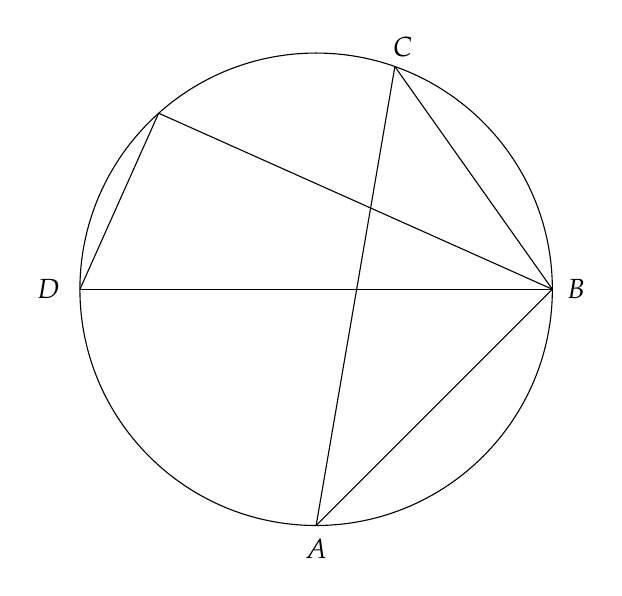
\begin{tikzpicture}[>=stealth,scale=1.0]
                \draw (0,0) circle(3);
                \draw[solid] (-3,0)--(3,0);
                \draw[solid] (-3,0)--(-2,2.236);
                \draw[solid] (3,0)--(-2,2.236);
                \draw[solid] (1,2.828)--(3,0);
                \draw[solid] (1,2.828)--(0,-3);
                \draw[solid] (3,0)--(0,-3);
                \node at(3.3,0) {$B$};
                \node at(0,-3.3) {$A$};
                \node at(1.1,3.078) {$C$};
                \node at(-3.4,0) {$D$};
            \end{tikzpicture}
            \caption{正弦定理的扩充示意图}
        \end{center}
    \end{figure}\\
    代入正弦定理,我们总共可以得出三组类似的结论。\\[3mm]
    \textbf{正弦定理的扩充:}
    \begin{large}
        \begin{align*}
            &2R=\frac{a}{\sin{A}}\\[3mm]
            &2R=\frac{b}{\sin{B}}\\[3mm]
            &2R=\frac{c}{\sin{C}}
        \end{align*}
    \end{large}

\newpage

\section{三角函数}

\subsection{正弦函数}
    \begin{figure}[h]
    \begin{center}
        \begin{tikzpicture}[>=stealth,scale=1.2]
            % draw the axis
            \draw[->] (-2*pi,0) -- (2*pi,0) node[above] {$x$};
            \draw[->] (0,-2) -- (0,2) node[right] {$y$};
            \foreach \x/\xt in {-2/-2\pi,-1/-\pi,1/\pi,2/2\pi}
                \draw[shift={(\x*pi,0)}] (0,0.1) -- (0,-0.1) node[below] {$\xt$};
            \foreach \y in {-2,-1,...,2}
                \draw[shift={(0,\y)}] (0.1,0) -- (-0.1,0) node[left] {$\y$};
            \draw[orange,smooth,thick,samples=100,domain=-2*pi:2*pi] 
                plot(\x,{sin(\x r)}) node at (2,1.5){$y=\sin{(x)}$};
        \end{tikzpicture}
        \caption{正弦函数的图像}
    \end{center}
    \end{figure}

    \textbf{正弦函数的性质:}\\[4mm]
    周期:$2\pi$\qquad
    定义域:$(-\infty,\infty)$\qquad
    值域:$[-1,1]$\\[5mm]
    与$x$轴交点:
    $\left\{x\mid x=k\cdot\pi,k\in\mathbb{Z}\right\}$\\[6mm]
    最大值:
    $\left\{x\mid x=k\cdot2\pi+\dfrac{\pi}{2},k\in\mathbb{Z}\right\}$\\[6mm]
    最小值:
    $\left\{x\mid x=k\cdot2\pi-\dfrac{\pi}{2},k\in\mathbb{Z}\right\}$\\[8mm]
    观察图形可以发现,正弦函数的本质是余弦函数向右平移$\dfrac{\pi}{2}$。

\newpage

\subsection{余弦函数}
    \begin{figure}[h]
    \begin{center}
        \begin{tikzpicture}[>=stealth,scale=1.2]
            % draw the axis
            \draw[->] (-2*pi,0) -- (2*pi,0) node[above] {$x$};
            \draw[->] (0,-2) -- (0,2) node[right] {$y$};
            \foreach \x/\xt in {-2/-2\pi,-1/-\pi,1/\pi,2/2\pi}
                \draw[shift={(\x*pi,0)}] (0,0.1) -- (0,-0.1) node[below] {$\xt$};
            \foreach \y in {-2,-1,...,2}
                \draw[shift={(0,\y)}] (0.1,0) -- (-0.1,0) node[left] {$\y$};
            \draw[cyan,smooth,thick,samples=100,domain=-2*pi:2*pi] 
                plot(\x,{cos(\x r)}) node at (2,1.5){$y=\cos{(x)}$};
        \end{tikzpicture}
        \caption{余弦函数的图像}
    \end{center}
    \end{figure}

    \textbf{余弦函数的性质:}\\[4mm]
    周期:$2\pi$\qquad
    定义域:$(-\infty,\infty)$\qquad
    值域:$[-1,1]$\\[5mm]
    与$x$轴交点:
    $\left\{x\mid x=k\cdot\pi+\dfrac{\pi}{2},k\in\mathbb{Z}\right\}$\\[6mm]
    最大值:
    $\left\{x\mid x=k\cdot2\pi,k\in\mathbb{Z}\right\}$\\[6mm]
    最小值:
    $\left\{x\mid x=k\cdot2\pi+\pi,k\in\mathbb{Z}\right\}$\\[8mm]
    观察图形可以发现,余弦函数的本质是正弦函数向左平移$\dfrac{\pi}{2}$。

\newpage

\subsection{关于函数$A\cdot\sin{(\omega\cdot x+\varphi)}$}

\subsubsection{参数$A$的意义}
    \begin{figure}[h]
    \begin{center}
        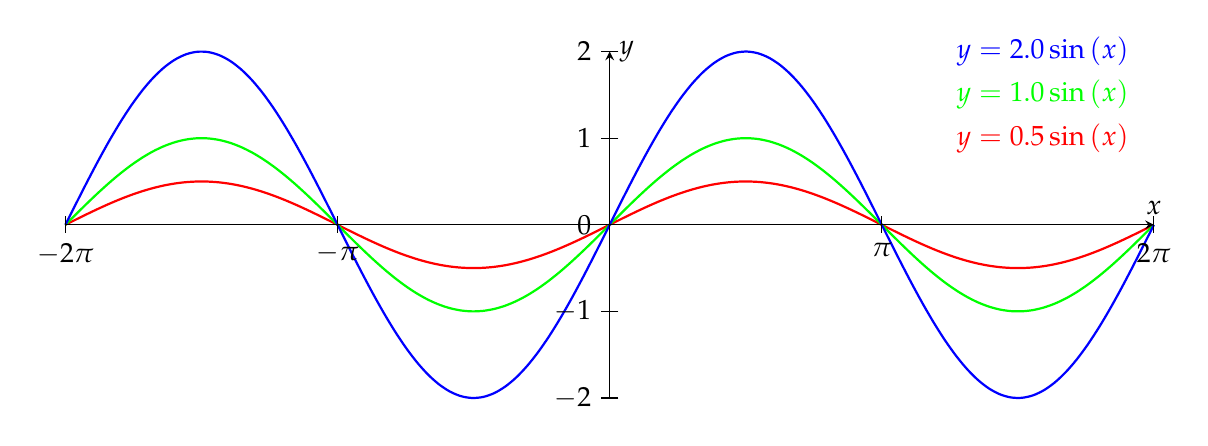
\begin{tikzpicture}[>=stealth,scale=1.1]
            \draw[red,smooth,thick,samples=100,domain=-2*pi:2*pi] 
                plot(\x,{0.5*sin(\x r)}) node at (5,1){$y=0.5\sin{(x)}$};
            \draw[green,smooth,thick,samples=100,domain=-2*pi:2*pi] 
                plot(\x,{1.0*sin(\x r)}) node at (5,1.5){$y=1.0\sin{(x)}$};
            \draw[blue,smooth,thick,samples=100,domain=-2*pi:2*pi] 
                plot(\x,{2.0*sin(\x r)}) node at (5,2){$y=2.0\sin{(x)}$};
            \draw[->] (-2*pi,0) -- (2*pi,0) node[above] {$x$};
            \draw[->] (0,-2) -- (0,2) node[right] {$y$};
            \foreach \x/\xt in {-2/-2\pi,-1/-\pi,1/\pi,2/2\pi}
                \draw[shift={(\x*pi,0)}] (0,0.1) -- (0,-0.1) node[below] {$\xt$};
            \foreach \y in {-2,-1,...,2}
                \draw[shift={(0,\y)}] (0.1,0) -- (-0.1,0) node[left] {$\y$};
        \end{tikzpicture}
        \caption{参数$A$对于正弦函数图像的影响}
    \end{center}
    \end{figure}
    参数$A$决定了图像在$y$轴上的缩放,缩放倍数为:$A$\\[5mm]
    参数$A$同时决定了函数的值域:$[-A,A]$\\

\subsubsection{参数$\omega$的意义}
    \begin{figure}[h]
    \begin{center}
        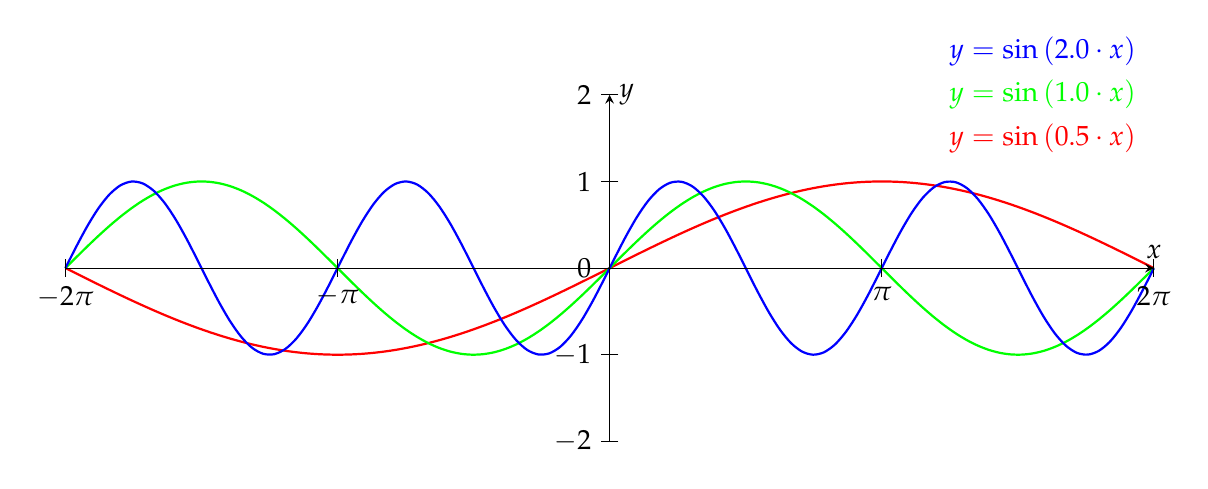
\begin{tikzpicture}[>=stealth,scale=1.1]
            \draw[red,smooth,thick,samples=100,domain=-2*pi:2*pi] 
                plot(\x,{sin(0.5*\x r)}) node at (5,1.5){$y=\sin{(0.5\cdot x)}$};
            \draw[green,smooth,thick,samples=100,domain=-2*pi:2*pi] 
                plot(\x,{sin(1.0*\x r)}) node at (5,2.0){$y=\sin{(1.0\cdot x)}$};
            \draw[blue,smooth,thick,samples=100,domain=-2*pi:2*pi] 
                plot(\x,{sin(2.0*\x r)}) node at (5,2.5){$y=\sin{(2.0\cdot x)}$};
            \draw[->] (-2*pi,0) -- (2*pi,0) node[above] {$x$};
            \draw[->] (0,-2) -- (0,2) node[right] {$y$};
            \foreach \x/\xt in {-2/-2\pi,-1/-\pi,1/\pi,2/2\pi}
                \draw[shift={(\x*pi,0)}] (0,0.1) -- (0,-0.1) node[below] {$\xt$};
            \foreach \y in {-2,-1,...,2}
                \draw[shift={(0,\y)}] (0.1,0) -- (-0.1,0) node[left] {$\y$};
        \end{tikzpicture}
        \caption{参数$\omega$对于正弦函数图像的影响}
    \end{center}
    \end{figure}
    参数$\omega$决定了图像在$x$轴上的缩放,缩放倍数为:$\dfrac{1}{\omega}$\\[3mm]
    参数$\omega$同时影响了图像的周期:$T=\dfrac{2\pi}{\omega}$

\newpage

\subsubsection{参数$\varphi$的意义}
    \begin{figure}[h]
    \begin{center}
        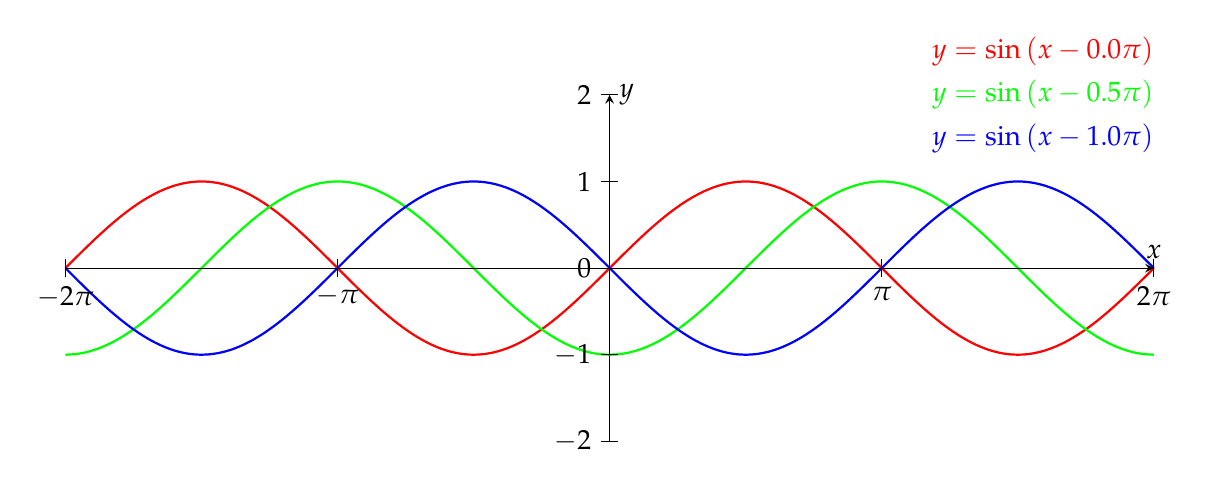
\begin{tikzpicture}[>=stealth,scale=1.1]
            \draw[red,smooth,thick,samples=100,domain=-2*pi:2*pi] 
                plot(\x,{sin(\x r)}) node at (5,2.5){$y=\sin{(x-0.0\pi)}$};
            \draw[green,smooth,thick,samples=100,domain=-2*pi:2*pi] 
                plot(\x,{sin((\x-0.5*pi) r)}) node at (5,2.0){$y=\sin{(x-0.5\pi)}$};
            \draw[blue,smooth,thick,samples=100,domain=-2*pi:2*pi] 
                plot(\x,{sin((\x-1.0*pi) r)}) node at (5,1.5){$y=\sin{(x-1.0\pi)}$};
            \draw[->] (-2*pi,0) -- (2*pi,0) node[above] {$x$};
            \draw[->] (0,-2) -- (0,2) node[right] {$y$};
            \foreach \x/\xt in {-2/-2\pi,-1/-\pi,1/\pi,2/2\pi}
                \draw[shift={(\x*pi,0)}] (0,0.1) -- (0,-0.1) node[below] {$\xt$};
            \foreach \y in {-2,-1,...,2}
                \draw[shift={(0,\y)}] (0.1,0) -- (-0.1,0) node[left] {$\y$};
        \end{tikzpicture}
        \caption{参数$\varphi$对于正弦函数图像的影响}
    \end{center}
    \end{figure}
    \begin{figure}[h]
    \begin{center}
        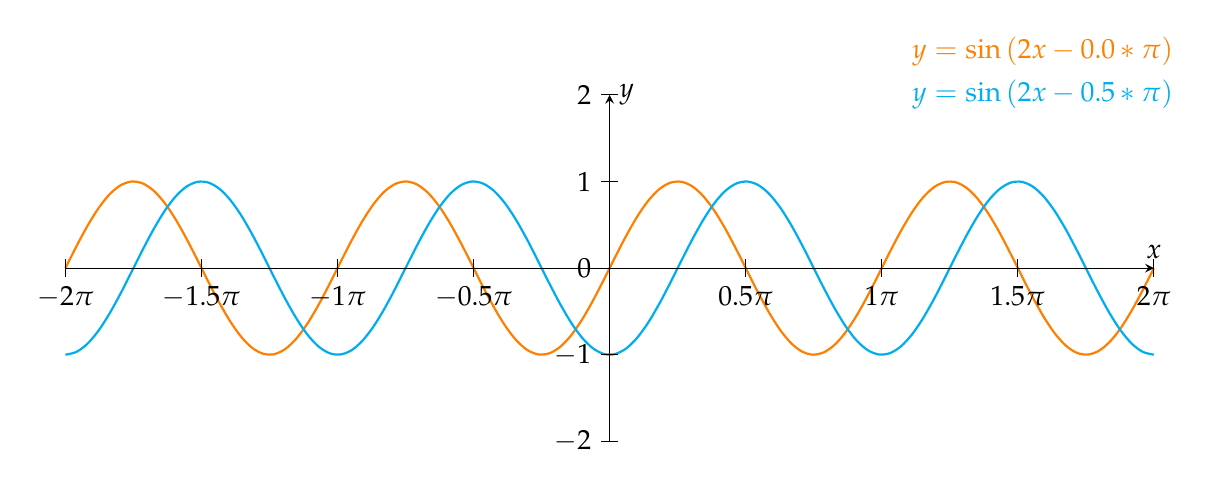
\begin{tikzpicture}[>=stealth,scale=1.1]
            \draw[orange,smooth,thick,samples=100,domain=-2*pi:2*pi] 
                plot(\x,{sin((2*\x) r)}) node at (5,2.5){$y=\sin{(2x-0.0*\pi)}$};
            \draw[cyan,smooth,thick,samples=100,domain=-2*pi:2*pi] 
                plot(\x,{sin((2*\x-0.5*pi) r)}) node at (5,2.0){$y=\sin{(2x-0.5*\pi)}$};
            \draw[->] (-2*pi,0) -- (2*pi,0) node[above] {$x$};
            \draw[->] (0,-2) -- (0,2) node[right] {$y$};
            \foreach \x/\xt in {-2/-2\pi,-1.5/-1.5\pi,-1/-1\pi,-0.5/-0.5\pi,0.5/0.5\pi,1/1\pi,1.5/1.5\pi,2/2\pi}
                \draw[shift={(\x*pi,0)}] (0,0.1) -- (0,-0.1) node[below] {$\xt$};
            \foreach \y in {-2,-1,...,2}
                \draw[shift={(0,\y)}] (0.1,0) -- (-0.1,0) node[left] {$\y$};
        \end{tikzpicture}
        \caption{参数$\omega$和参数$\varphi$对于平移的影响}
    \end{center}
    \end{figure}\vspace{5pt}
    参数$\varphi$和参数$\omega$共同决定了图像在$x$轴上的平移:$-\dfrac{\varphi}{\omega}$

\newpage

\subsection{正切函数}
    \begin{figure}[h]
    \begin{center}
        \begin{tikzpicture}[>=stealth,scale=1.1]
            % draw the axis
            \draw[->] (-2.3*pi,0) -- (2.3*pi,0) node[above] {$x$};
            \draw[->] (0,-5.5) -- (0,5.5) node[right] {$y$};
            \foreach \x/\xt in {-2/-2\pi,-1/-\pi,1/\pi,2/2\pi}
                \draw[shift={(\x*pi,0)}] (0,0.1) -- (0,-0.1) node[below] {$\xt$};
            \foreach \y in {-5,-4,...,5}
                \draw[shift={(0,\y)}] (0.1,0) -- (-0.1,0) node[left] {$\y$};
            \foreach \m in {-1,0,1}
                \draw[orange,smooth,thick,samples=100,domain=\m*pi-pi/2+pi/16:\m*pi+pi/2-pi/16] 
                plot(\x,{tan((\x) r)});
            \draw[orange] node at (2.5,2.5){$y=\tan{(x)}$};
        \end{tikzpicture}
        \caption{正切函数的图像}
    \end{center}
    \end{figure}
    \textbf{正切函数的性质:}\\[4mm]
    周期:$\pi$\qquad
    定义域:$\left\{x\mid x\neq k\cdot\pi+\dfrac{\pi}{2},k\in\mathbb{Z}\right\}$\qquad
    值域:$(-\infty,\infty)$\\[6mm]
    与$x$轴交点:
    $\left\{x\mid x=k\cdot\pi,k\in\mathbb{Z}\right\}$\\[6mm]
    正切函数的图像在局部是单调递增的。\\[8mm]
    观察图像可以发现,
    正切函数的本质是余切函数向右平移$\dfrac{\pi}{2}$,
    再关于$y$轴翻转。

\newpage

\subsection{余切函数}
    \begin{figure}[h]
    \begin{center}
        \begin{tikzpicture}[>=stealth,scale=1.1]
            % draw the axis
            \draw[->] (-2.3*pi,0) -- (2.3*pi,0) node[above] {$x$};
            \draw[->] (0,-5.5) -- (0,5.5) node[right] {$y$};
            \foreach \x/\xt in {-2/-2\pi,-1/-\pi,1/\pi,2/2\pi}
                \draw[shift={(\x*pi,0)}] (0,0.1) -- (0,-0.1) node[below] {$\xt$};
            \foreach \y in {-5,-4,...,5}
                \draw[shift={(0,\y)}] (0.1,0) -- (-0.1,0) node[left] {$\y$};
            \foreach \m in {-2,-1,...,1}
                \draw[cyan,smooth,thick,samples=100,domain=\m*pi+0+pi/16:\m*pi+pi-pi/16] 
                plot(\x,{cot((\x) r)});
            \draw[cyan] node at (2.5,2.5){$y=\cot{(x)}$};
        \end{tikzpicture}
        \caption{余切函数的图像}
    \end{center}
    \end{figure}
    \textbf{余切函数的性质:}\\[4mm]
    周期:$\pi$\qquad
    定义域:$\left\{x\mid x\neq k\cdot\pi,k\in\mathbb{Z}\right\}$\qquad
    值域:$(-\infty,\infty)$\\[6mm]
    与$x$轴交点:
    $\left\{x\mid x\neq k\cdot\pi+\dfrac{\pi}{2},k\in\mathbb{Z}\right\}$\\[6mm]
    余切函数的图像在局部是单调递减的。\\[8mm]
    观察图像可以发现,
    余切函数的本质是正切函数向左平移$\dfrac{\pi}{2}$,
    再关于$y$轴翻转。

\newpage

\subsection{反正弦函数}
    \begin{figure}[h]
    \begin{center}
        \begin{tikzpicture}[>=stealth,scale=1.1]
            \draw[orange,smooth,thick,samples=100,domain=-1:1] 
                plot(\x,{asin(\x)/180*pi}) node at (1.5,2.0){$y=\arcsin{(x)}$};
            \draw[->] (-3.5,0) -- (3.5,0) node[below] {$x$};
            \draw[->] (0,-0.7*pi) -- (0,0.7*pi) node[right] {$y$};
            \foreach \x in {-3,-2,-1,1,2,3}
                \draw[shift={(\x,0)}] (0,0.1) -- (0,-0.1) node[below] {$\x$};
            \foreach \y/\yt in {-0.5/-0.5\pi,0.5/0.5\pi}
                \draw[shift={(0,pi*\y)}] (0.1,0) -- (-0.1,0) node[left] {$\yt$};
        \end{tikzpicture}
        \caption{反正弦函数的图像}
    \end{center}
    \end{figure}
    \textbf{反正弦函数的性质:}\\[3mm]
    定义域:$[-1,1]$\\[3mm]
    值域:$[-\dfrac{\pi}{2},\dfrac{\pi}{2}]$\\[4mm]

\subsection{反余弦函数}
    \begin{figure}[h]
    \begin{center}
        \begin{tikzpicture}[>=stealth,scale=1.1]
            \draw[cyan,smooth,thick,samples=100,domain=-1:1] 
                plot(\x,{acos(\x)/180*pi}) node at (1.5,2.5){$y=\arccos{(x)}$};
            \draw[->] (-3.5,0) -- (3.5,0) node[below] {$x$};
            \draw[->] (0,-0.7) -- (0,1.2*pi) node[right] {$y$};
            \foreach \x in {-3,-2,-1,1,2,3}
                \draw[shift={(\x,0)}] (0,0.1) -- (0,-0.1) node[below] {$\x$};
            \foreach \y/\yt in {0.5/0.5\pi,1/1.0\pi}
                \draw[shift={(0,pi*\y)}] (0.1,0) -- (-0.1,0) node[left] {$\yt$};
        \end{tikzpicture}
        \caption{反余弦函数的图像}
    \end{center}
    \end{figure}
    \textbf{反余弦函数的性质:}\\[3mm]
    定义域:$[-1,1]$\\[3mm]
    值域:$[0,\pi]$

\subsection{反正切函数}
    \begin{figure}[h]
    \begin{center}
        \begin{tikzpicture}[>=stealth,scale=1.1]
            \draw[orange,smooth,thick,samples=100,domain=-5:5] 
                plot(\x,{atan(\x)/180*pi}) node at (2.0,1.8){$y=\arctan{(x)}$};
            \draw[->] (-5.5,0) -- (5.5,0) node[below] {$x$};
            \draw[->] (0,-0.7*pi) -- (0,0.7*pi) node[right] {$y$};
            \foreach \x in {-5,-4,-3,-2,-1,1,2,3,4,5}
                \draw[shift={(\x,0)}] (0,0.1) -- (0,-0.1) node[below] {$\x$};
            \foreach \y/\yt in {-0.5/-0.5\pi,0.5/0.5\pi}
                \draw[shift={(0,pi*\y)}] (0.1,0) -- (-0.1,0) node[left] {$\yt$};
        \end{tikzpicture}
        \caption{反正切函数的图像}
    \end{center}
    \end{figure}
    \textbf{反正切函数的性质:}\\[3mm]
    定义域:$(-\infty,\infty)$\\[3mm]
    值域:$(-\dfrac{\pi}{2},\pi)$\\[3mm]

\subsection{反余切函数}
    \begin{figure}[h]
    \begin{center}
        \begin{tikzpicture}[>=stealth,scale=1.1]
            \draw[cyan,smooth,thick,samples=100,domain=-5:5]
                plot(\x,{pi/2-(atan(\x)/180*pi)}) node at (2.0,1.8){$y=\arccot{(x)}$};
            \draw[->] (-5.5,0) -- (5.5,0) node[below] {$x$};
            \draw[->] (0,-0.3*pi) -- (0,1.3*pi) node[right] {$y$};
            \foreach \x in {-5,-4,-3,-2,-1,1,2,3,4,5}
                \draw[shift={(\x,0)}] (0,0.1) -- (0,-0.1) node[below] {$\x$};
            \foreach \y/\yt in {0.5/0.5\pi,1.0/1.0\pi}
                \draw[shift={(0,pi*\y)}] (0.1,0) -- (-0.1,0) node[left] {$\yt$};
        \end{tikzpicture}
        \caption{反余切函数的图像}
    \end{center}
    \end{figure}
    \textbf{反余切函数的性质:}\\[3mm]
    定义域:$(-\infty,\infty)$\\[3mm]
    值域:$(0,\pi)$

\newpage

\section{数列}
    递推公式形容了数列中任意一项与其前一项之间的关系。\\[3mm]
    通项公式形容了数列中任意一项与其序数的关系。

\subsection{等差数列}
    等差数列中,相邻项之间的差等于一个常数,
    这个常数称为公差,通常用$d$表述。

\subsubsection{等差数列的递推公式}
    根据等差数列的定义,我们可以得到等差数列的递推公式:
    \begin{large}
    \begin{equation*}
        a_n=a_{n-1}+d
    \end{equation*}    
    \end{large}

\subsubsection{等差数列的通项公式}
    通过递推公式,我们可以得到等差数列的通项公式:
    \begin{large}
    \begin{equation*}
        a_n=a_1+(n-1)\cdot d
    \end{equation*}
    \end{large}

\subsubsection{等差数列的求和公式}
    等差数列的求和公式通常可以表述为以下三种形式:\\[4mm]
    关于首项和末项:
    \begin{large}
    \begin{equation*}
        S_n=\frac{(a_1+a_n)\cdot n}{2}
    \end{equation*}
    \end{large}\\
    关于首项和公差:
    \begin{large}
    \begin{equation*}
        S_n=n\cdot a_1+\frac{(n^2-n)}{2}\cdot d
    \end{equation*}
    \end{large}\\
    关于序数:
    \begin{large}
    \begin{equation*}
        S_n=\frac{d}{2}\cdot n^2+(a_1-\frac{d}{2})\cdot n
    \end{equation*}
    \end{large}

\newpage

\subsection{等比数列}
    等比数列中,相邻项之间的比等于一个常数,
    这个常数称为公比,通常用$q$来表达。

\subsubsection{等比数列的递推公式}
    根据等比数列的定义,我们可以得到等比数列的递推公式:
    \begin{large}
    \begin{equation*}
        a_n=a_{n-1}\cdot q
    \end{equation*}    
    \end{large}

\subsubsection{等比数列的通项公式}
    通过递推公式,我们可以得到等比数列的通项公式:
    \begin{large}
    \begin{equation*}
        a_n=a_1\cdot q^{n-1}
    \end{equation*}
    \end{large}

\subsubsection{等比数列的求和公式}
    当$q\neq1$时:
    \begin{large}
    \begin{equation*}
        S_n=\frac{a_1\cdot(1-q^n)}{1-q}=\frac{a_1-a_n\cdot q}{1-q}
    \end{equation*}
    \end{large}\\
    当$q=1$时:
    \begin{large}
    \begin{equation*}
        S_n=n\cdot a_1
    \end{equation*}
    \end{large}\\

\subsection{通过递推公式推导通项公式}

\subsubsection{形如{\large$a_{n+1}=a_n+f(n)$}}
    通过递推公式,
    我们可以得到相邻两项的差关于$n$的表达式,
    所以可以运用累加法:
    \begin{large}
    \begin{equation*}
        a_n=a_1+\sum_{x=1}^{n-1}f(x)
    \end{equation*}
    \end{large}

\subsubsection{形如{\large$a_{n+1}=a_n\times f(n)$}}
    通过递推公式,
    我们可以得到相邻两项的比关于$n$的表达式,
    所以可以运用累乘法:
    \begin{large}
    \begin{equation*}
        a_n=a_1\times\prod_{x=1}^{n-1}f(x)
    \end{equation*}
    \end{large}

\newpage

\subsubsection{形如{\large$a_{n+1}=q\cdot a_{n}+c$}}
    运用待定系数法,我们可以进行如下推导:
    \setcounter{equation}{0}
    \begin{align}
        &a_{n+1}=q\cdot a_n+c\\[2mm]
        &a_{n+1}+x=q\cdot(a_n+x)\\[2mm]
        &a_{n+1}+x=q\cdot a_n+q\cdot x\\[2mm]
        &a_{n+1}=q\cdot a_n+(q-1)\cdot x
    \end{align}\\
    与原式对照可以得到:
    \begin{align}
        &(q-1)\cdot x=c\\[3mm]
        &x=\frac{c}{q-1}
    \end{align}\\
    代入可得:
    \begin{align}
        &a_{n+1}+\frac{c}{q-1}=\left(a_n+\frac{c}{q-1}\right)\cdot q\\[3mm]
        &a_{n+1}+\frac{c}{q-1}=\left(a_1+\frac{c}{q-1}\right)\cdot q^n\\[3mm]
        &a_{n+1}+\frac{c}{q-1}=a_1\cdot q^n+\frac{c}{q-1}\cdot q^n\\[3mm]
        &a_{n+1}=a_1\cdot q^n+\frac{c}{q-1}\cdot (q^n-1)
    \end{align}\\
    用$n$替代$n+1$后,我们就可以得到通项公式:
    \begin{large}
    \begin{equation*}
        a_{n}=q^{n-1}\cdot a_1+\frac{c}{q-1}\cdot (q^{n-1}-1)
    \end{equation*}
    \end{large}

\newpage

\subsubsection{形如{\large$a_{n+1}=q\cdot a_n+c^n$}}
    首先两边同除$c^{n+1}$:
    \setcounter{equation}{0}
    \begin{align}
        &a_{n+1}=q\cdot a_n+c^n\\[3mm]
        &\frac{a_{n+1}}{c^{n+1}}=\frac{q\cdot a_n}{c^{n+1}}+\frac{1}{c}\\[3mm]
        &\frac{a_{n+1}}{c^{n+1}}=\frac{q}{c}\cdot \frac{a_n}{c^n}+\frac{1}{c}
    \end{align}\\
    令$b_n=\dfrac{a_n}{c^n}$,使用待定系数法的公式:
    \begin{align}
        &b_{n+1}=\frac{q}{c}\cdot b_n+\frac{1}{c}\\[3mm]
        &b_{n+1}=b_1\cdot\left(\frac{q}{c}\right)^n+\left(\frac{\dfrac{1}{c}}{\dfrac{q}{c}-1}\right)\cdot\left[\left(\frac{q}{c}\right)^n-1\right]\\[3mm]
        &b_{n+1}=b_1\cdot\left(\frac{q}{c}\right)^n+\left(\frac{\dfrac{1}{c}}{\dfrac{q-c}{c}}\right)\cdot\left[\left(\frac{q}{c}\right)^n-1\right]\\[3mm]
        &b_{n+1}=b_1\cdot\left(\frac{q}{c}\right)^n+\left(\frac{1}{c}\cdot\frac{c}{q-c}\right)\cdot\left[\left(\frac{q}{c}\right)^n-1\right]\\[3mm]
        &b_{n+1}=b_1\cdot\left(\frac{q}{c}\right)^n+\frac{1}{q-c}\cdot\left[\left(\frac{q}{c}\right)^n-1\right]\\[3mm]
        &\frac{a_{n+1}}{c^{n+1}}=\frac{a_1}{c}\cdot\frac{q^n}{c^n}+\frac{1}{q-c}\cdot\left(\frac{q^n}{c^n}-1\right)\\[3mm]
        &\frac{a_{n+1}}{c^{n+1}}=\frac{a_1\cdot q^n}{c^{n+1}}+\frac{1}{q-c}\cdot\left(\frac{q^n}{c^n}-1\right)\\[3mm]
        &a_{n+1}=a_1\cdot q^n+\frac{1}{q-c}\cdot\left(\frac{q^n}{c^n}-1\right)\cdot c^{n+1}\\[3mm]
        &a_{n+1}=a_1\cdot q^n+\frac{1}{q-c}\cdot\left(q^n\cdot c-c^{n+1}\right)\\[3mm]
        &a_{n+1}=a_1\cdot q^n+\frac{c}{q-c}\cdot\left(q^n-c^{n}\right)
    \end{align}\\
    用$n$替代$n+1$后,我们就可以得到通项公式:
    \begin{large}
    \begin{equation*}
        a_{n}=q^{n-1}\cdot a_1+\frac{c}{q-c}\cdot\left(q^{n-1}-c^{n-1}\right)
    \end{equation*}
    \end{large}

\newpage

\subsubsection{形如{\large$a_{n+1}=q\cdot a_n^{~c}$}}
    等式两边取对数:
    \setcounter{equation}{0}
    \begin{align}
        &a_{n+1}=q\cdot a_n^c\\[3mm]
        &\lg{a_{n+1}}=c\cdot \lg{q}+\lg{a_n}\\[3mm]
        &\lg{a_{n+1}}=c\cdot \lg{a_n}+\lg{q}
    \end{align}\\
    令$b_n=\lg{a_n}$,使用待定系数法的公式:
    \begin{align}
        &b_{n+1}=c\cdot b_n+\lg{q}\\[3mm]
        &b_{n+1}=c^n\cdot b_1+\frac{\lg{q}}{c-1}\cdot\left(c^n-1\right)\\[3mm]
        &\lg{a_{n+1}}=c^n\cdot \lg{a_1}+\frac{\lg{q}}{c-1}\cdot\left(c^n-1\right)\\[3mm]
        &\lg{a_{n+1}}=\lg{a_1^{~c^{n}}}+lg{q^{\frac{c^n-1}{c-1}}}\\[3mm]
        &\lg{a_{n+1}}=\lg{a_1^{~c^{n}}\cdot q^{\frac{c^n-1}{c-1}}}\\[3mm]
        &a_{n+1}=a_1^{~c^{n}}\cdot q^{\frac{c^n-1}{c-1}}
    \end{align}\\
    用$n$替代$n+1$后,我们就可以得到通项公式:
    \begin{large}
    \begin{equation*}
        a_{n}=a_1^{~c^{n-1}}\cdot q^{\frac{c^{n-1}-1}{c-1}}
    \end{equation*}
    \end{large}

\newpage

\subsubsection[形如{\large $a_{n+1}=(p\cdot a_n)/(q\cdot a_n+c)$}]{形如{\large$a_{n+1}=\dfrac{p\cdot a_n}{q\cdot a_n+c}$}}
    等式两边取倒数:
    \setcounter{equation}{0}
    \begin{align}
        &a_{n+1}=\frac{p\cdot a_n}{q\cdot a_n+c}\\[3mm]
        &\frac{1}{a_{n+1}}=\frac{q\cdot a_n+c}{p\cdot a_n}\\[3mm]
        &\frac{1}{a_{n+1}}=\frac{q}{p}+\frac{c}{p\cdot an}\\[3mm]
        &\frac{1}{a_{n+1}}=\frac{c}{p}\cdot\frac{1}{a_{n}}+\frac{q}{p}\\[3mm]
    \end{align}\\
    令$b_n=\dfrac{1}{a_n}$,使用待定系数法的公式:
    \begin{align}
        &b_{n+1}=\frac{c}{p}\cdot b_{n+1}+\frac{q}{p}\\[3mm]
        &b_{n+1}=\left(\frac{c}{p}\right)^n\cdot b_1+\frac{\dfrac{q}{p}}{\dfrac{c}{p}-1}\cdot\left[\left(\frac{c}{p}\right)^n-1\right]\\[3mm]
        &b_{n+1}=\frac{c^n}{p^n}\cdot b_1+\frac{\dfrac{q}{p}}{\dfrac{c-p}{p}}\cdot\left(\frac{c^n}{p^n}-1\right)\\[3mm]
        &b_{n+1}=\frac{c^n}{p^n}\cdot b_1+\frac{q}{c-p}\cdot\left(\frac{c^n}{p^n}-1\right)\\[3mm]
        &\frac{1}{a_{n+1}}=\frac{c^n}{p^n}\cdot\frac{1}{a_1}+\frac{q}{c-p}\cdot\left(\frac{c^n}{p^n}-1\right)\\[3mm]
        &a_{n+1}=\frac{1}{\dfrac{c^n}{p^n}\cdot\dfrac{1}{a_1}+\dfrac{q}{c-p}\cdot\left(\dfrac{c^n}{p^n}-1\right)}
    \end{align}\\
    用$n$替代$n+1$后,我们就可以得到通项公式:\\
    \begin{large}
    \begin{equation*}
        a_{n}=\frac{1}{\dfrac{c^{n-1}}{p^{n-1}}\cdot\dfrac{1}{a_1}+\dfrac{q}{c-p}\cdot\left(\dfrac{c^{n-1}}{p^{n-1}}-1\right)}
    \end{equation*}
    \end{large}
\newpage

\subsubsection{形如{\large$a_{n+1}+a_{n}=f(n)$}}
    通过以下推导:
    \setcounter{equation}{0}
    \begin{align}
        &a_{n+1}+a_{n}=f(n)\\[3mm]
        &a_{n+2}+a_{n+1}=f(n+1)\\[5mm]
        &a_{n+2}+a_{n+1}-a_{n+1}-an=f(n+1)-f(n)\\[3mm]
        &a_{n+2}-a_{n}=f(n+1)-f(n)
    \end{align}
    当n为奇数时:
    \begin{large}
    \begin{equation*}
        a_n=a_1+\sum_{x=1}^{\frac{n-1}{2}}\left(f(2x)-f(2x-1)\right)
    \end{equation*}
    \end{large}\\
    对于奇数,可以这样理解:\\[3mm]
    函数所需的参数\{n\}:$1~3~5~\cdots~n-2$\\[3mm]
    求和所提供的数\{x\}:$1~2~3~\cdots~\dfrac{n-1}{2}$\\[3mm]
    两者的关系:$n=2x-1$\\[3mm]
    $f(n+1)=f(2x-1+1)=f(2x)$\qquad
    $f(n)=f(2x-1)$\\[6mm]
    当n为偶数时:
    \begin{large}
    \begin{equation*}
        a_n=a_1+\sum_{x=1}^{\frac{n-2}{2}}\left(f(2x+1)-f(2x)\right)
    \end{equation*}
    \end{large}\\
    对于偶数,可以这样理解:\\[3mm]
    函数所需的参数\{n\}:$2~4~6~\cdots~n-2$\\[3mm]
    求和所提供的数\{x\}:$1~2~3~\cdots~\dfrac{n-2}{2}$\\[3mm]
    两者的关系:$n=2x$\\[3mm]
    $f(n+1)=f(2x+1)$\qquad
    $f(n)=f(2x)$
    
\newpage

\subsubsection{形如{\large$a_{n+1}\times a_{n}=f(n)$}}
    通过以下推导:
    \setcounter{equation}{0}
    \begin{align}
        &a_{n+1}\cdot a_{n}=f(n)\\[3mm]
        &a_{n+2}\cdot a_{n+1}=f(n+1)\\[5mm]
        &\frac{a_{n+2}\cdot a_{n+1}}{a_{n+1}\cdot a_n}=\frac{f(n+1)}{f(n)}\\[3mm]
        &\frac{a_{n+2}}{a_n}=\frac{f(n+1)}{f(n)}
    \end{align}
    当n为奇数时:
    \begin{large}
    \begin{equation*}
        a_n=a_1\times\prod_{x=1}^{\frac{n-1}{2}}\frac{f(2x)}{f(2x-1)}
    \end{equation*}
    \end{large}\\
    对于奇数,可以这样理解:\\[3mm]
    函数所需的参数\{n\}:$1~3~5~\cdots~n-2$\\[3mm]
    求和所提供的数\{x\}:$1~2~3~\cdots~\dfrac{n-1}{2}$\\[3mm]
    两者的关系:$n=2x-1$\\[3mm]
    $f(n+1)=f(2x-1+1)=f(2x)$\qquad
    $f(n)=f(2x-1)$\\[6mm]
    当n为偶数时:
    \begin{large}
    \begin{equation*}
        a_n=a_1\times\prod_{x=1}^{\frac{n-2}{2}}\frac{f(2x+1)}{f(2x)}
    \end{equation*}
    \end{large}\\
    对于偶数,可以这样理解:\\[3mm]
    函数所需的参数\{n\}:$2~4~6~\cdots~n-2$\\[3mm]
    求和所提供的数\{x\}:$1~2~3~\cdots~\dfrac{n-2}{2}$\\[3mm]
    两者的关系:$n=2x$\\[3mm]
    $f(n+1)=f(2x+1)$\qquad
    $f(n)=f(2x)$

\newpage

\subsection{数列的极限}
    数列的极限可以通俗的理解为:对于一个数列$\{a_n\}$,
    在项数$n$无限增大的过程中项$a_{n}$无限趋近于的常数。
    但是这样的形象表述并不严谨,不符合数学的严密性和简洁性,
    也不利于证明过程的书写,所以我们需要对数列的极限进行严格的定义。\\[3mm]
    \textbf{数列极限的$\varepsilon-N$定义:}
    设$\{a_n\}$是一个数列,如果存在常数$a$,
    对于任意给定的正数$\varepsilon$,
    总存在一个正整数$N$,使得当$n>N$时,
    都有$\left|a_n-A\right|<\varepsilon$,
    则称数列$\{a_n\}$的极限是A。
    \begin{large}
        \begin{equation*}
            \lim_{n\to\infty}a_n=A
        \end{equation*}
    \end{large}\\
    如果一个数列$\{a_n\}$存在极限,我们也可以说数列${a_n}$是收敛的。\\[2mm]
    如果一个数列$\{a_n\}$不存在极限,我们也可以说数列${a_n}$是发散的。\\[5mm]
    常数列的极限等于常数自身:
    \begin{large}
        \begin{equation*}
            \lim_{x\to\infty}(C)=C
        \end{equation*}
    \end{large}\\
    两个数列和的极限等于它们的极限之和:
    \begin{large}
        \begin{equation*}
            \lim_{x\to\infty}[a_{n}+b_{n}]=\lim_{x\to\infty}a_{n}+\lim_{x\to\infty}b_{n}
        \end{equation*}
    \end{large}\\
    两个数列差的极限等于它们的极限之差:
    \begin{large}
        \begin{equation*}
            \lim_{x\to\infty}[a_{n}-b_{n}]=\lim_{x\to\infty}a_{n}-\lim_{x\to\infty}b_{n}
        \end{equation*}
    \end{large}\\
    两个数列积的极限等于它们的极限之积:
    \begin{large}
        \begin{equation*}
            \lim_{x\to\infty}[a_{n}\cdot b_{n}]=\lim_{x\to\infty}a_{n}\cdot\lim_{x\to\infty}b_{n}
        \end{equation*}
    \end{large}\\
    两个数列商的极限等于它们的极限之商:
    \begin{large}
        \begin{equation*}
            \lim_{x\to\infty}\frac{a_{n}}{b_{n}}=\frac{\lim\limits_{x\to\infty}a_{n}}{\lim\limits_{x\to\infty}b_{n}}\qquad\left(\lim_{x\to\infty}b_n\neq 0\right)
        \end{equation*}
    \end{large}\\


\newpage

\section{向量}
    标量指的是只有大小没有方向的量。\\[3mm]
    向量指的是既有大小又有方向的量。\\[3mm]
    在数学上,通常用有向线段形象的表示向量,其长度代表向量的长度,其角度代表向量的角度,
    由于向量并不关心位置,因此长度和角度相同但位置不同的有向线段代表的是同一个向量。

\subsection{向量的表示}
    特别的,我们将长度为$1$的向量称为单位向量。\\[6mm]
    在二维平面中,我们定义以下两个特殊的单位向量指向两个坐标轴的正方向:
    \begin{large}
        \begin{equation*}
            \vec{i}=(1,0)~~~~~~~~\vec{j}=(0,1)
        \end{equation*}
    \end{large}\\
    在二维平面中,任何一个向量都可以表示为上述两个单位向量的线性组合:
    \begin{large}
        \begin{align*}
            &\vec{a}=(x,y)\\[3mm]
            &\vec{a}=x\cdot\vec{i}+y\cdot\vec{j}
        \end{align*}
    \end{large}\\
    二维平面中的向量,我们通常称为平面向量。\\[12mm]
    在三维空间中,我们定义以下三个特殊的单位向量指向三个坐标轴的正方向:
    \begin{large}
        \begin{equation*}
            \vec{i}=(1,0,0)~~~~~~~~\vec{j}=(0,1,0)~~~~~~~~\vec{k}=(0,0,1)
        \end{equation*}
    \end{large}\\
    在三维空间中,任何一个向量都可以表示为上述两个单位向量的线性组合:
    \begin{large}
        \begin{align*}
            &\vec{a}=(x,y,z)\\[3mm]
            &\vec{a}=x\cdot\vec{i}+y\cdot\vec{j}+z\cdot\vec{k}
        \end{align*}
    \end{large}\\
    三维空间中的向量,我们通常称为空间向量。

\newpage

\subsection{向量的长度}
    向量的长度可以用向量的模表示。\\[3mm]
    平面向量的模:
    \begin{large}
        \begin{equation*}
            \left|\vec{a}\right|=\sqrt{x^2+y^2}    
        \end{equation*}
    \end{large}\\
    空间向量的模:
    \begin{large}
        \begin{equation*}
            \left|\vec{a}\right|=\sqrt{x^2+y^2+z^2}
        \end{equation*}
    \end{large}\vspace{-10pt}

\subsection{向量的角度}
    向量的角度可以用向量的单位向量表示。\\[3mm]
    平面向量的单位向量:
    \begin{large}
        \begin{equation*}
            \vec{a_0}=\left(\frac{x}{|\vec{a}|}~,~\frac{y}{|\vec{a}|}\right)
        \end{equation*}
    \end{large}\\
    空间向量的单位向量:
    \begin{large}
        \begin{equation*}
            \vec{a_0}=\left(\frac{x}{|\vec{b}|}~,~\frac{y}{|\vec{b}|}~,~\frac{z}{|\vec{b}|}\right)
        \end{equation*}
    \end{large}\vspace{-4pt}

\subsection{向量的加法}
    平面向量的加法:
    \begin{large}
        \begin{equation*}
            \vec{a}+\vec{b}=(x_1+x_2~,~y_1+y_2)
        \end{equation*}
    \end{large}\\
    空间向量的加法:
    \begin{large}
        \begin{equation*}
            \vec{a}+\vec{b}=(x_1+x_2~,~y_1+y_2~,~z_1+z_2)
        \end{equation*}
    \end{large}\vspace{-5pt}

\subsection{向量的减法}
    平面向量的减法:
    \begin{large}
        \begin{equation*}
            \vec{a}-\vec{b}=(x_1-x_2~,~y_1-y_2)
        \end{equation*}
    \end{large}\\
    空间向量的减法:
    \begin{large}
        \begin{equation*}
            \vec{a}-\vec{b}=(x_1-x_2~,~y_1-y_2~,~z_1-z_2)
        \end{equation*}
    \end{large}

\newpage

\subsection{向量的数乘}
    平面向量的数乘:
    \begin{large}
        \begin{equation*}
            \lambda\cdot\vec{a}=\left(\lambda\cdot x~,~\lambda\cdot y\right)
        \end{equation*}
    \end{large}\\
    空间向量的数乘:
    \begin{large}
        \begin{equation*}
            \lambda\cdot\vec{a}=\left(\lambda\cdot x~,~\lambda\cdot y~,~\lambda\cdot z\right)
        \end{equation*}
    \end{large}\\
    向量数乘的结合律:
    \begin{large}
        \begin{equation*}
            m\cdot n\cdot \vec{a}=m\cdot (n\cdot\vec{a})
        \end{equation*}
    \end{large}\\
    向量数乘的第一分配律:
    \begin{large}
        \begin{equation*}
            (m+n)\cdot\vec{a}=m\cdot\vec{a}+n\cdot\vec{a}
        \end{equation*}
    \end{large}\\
    向量数乘的第二分配律:
    \begin{large}
        \begin{equation*}
            m\cdot (\vec{a}+\vec{b})=m\cdot\vec{a}+m\cdot\vec{b}
        \end{equation*}
    \end{large}

\subsubsection{平面向量共线定理}
    如果两个平面向量满足以下条件:
    \begin{large}
        \begin{equation*}
            \vec{b}=\lambda\cdot \vec{a}
        \end{equation*}
    \end{large}\\
    那么这两个向量共线,且实数$\lambda$是唯一的。\\

\subsubsection{空间向量共面定理}
    如果两个平面向量满足以下条件:
    \begin{large}
        \begin{equation*}
            \vec{c}=\lambda\cdot \vec{a}+\mu\cdot \vec{b}
        \end{equation*}
    \end{large}\\
    那么这两个向量共线,且实数对$\lambda,\mu$是唯一的。

\newpage

\subsection{向量的点乘}
    向量的点乘:
    \begin{large}
        \begin{equation*}
            \vec{a}\cdot\vec{b}=|\vec{a}|\cdot|\vec{b}|\cdot\cos{\theta}
        \end{equation*}
    \end{large}\\
    需要指出的是,该公式对平面向量和空间向量,乃至更高维向量均是适用的。\\[6mm]
    向量点乘的交换律:
    \begin{large}
        \begin{equation*}
            \vec{a}\cdot\vec{b}=\vec{b}\cdot\vec{a}
        \end{equation*}
    \end{large}\\
    向量点乘的分配律:
    \begin{large}
        \begin{equation*}
            \vec{a}\cdot(\vec{b}+\vec{c})=\vec{a}\cdot\vec{b}+\vec{a}\cdot\vec{c}
        \end{equation*}
    \end{large}\\
    向量点乘\textbf{不符合}结合律,但有以下性质:
    \begin{large}
        \begin{equation*}
            \lambda\cdot\vec{a}\cdot\vec{b}=(\lambda\cdot\vec{a})\cdot\vec{b}=(\lambda\cdot\vec{b})\cdot\vec{a}
        \end{equation*}
    \end{large}\\
    推导平面向量点乘的坐标形式:
    \setcounter{equation}{0}
    \begin{align}
        \vec{a}\cdot\vec{b}
        &=(x_1\cdot\vec{i}+y_1\cdot\vec{j})\cdot(x_2\cdot\vec{i}+y_2\cdot\vec{j})\\[3mm]
        &=(x_1\cdot x_2)\cdot\vec{i}~^2+(y_1\cdot y_2)\cdot\vec{j}~^2+(x_1\cdot y_2+x_2\cdot y_1)\cdot\vec{i}\cdot\vec{j}\\[3mm]
        &=x_1\cdot x_2+y_1\cdot y_2
    \end{align}\\
    推导空间向量点乘的坐标形式:
    \setcounter{equation}{0}
    \begin{align}
        \vec{a}\cdot\vec{b}
        &=(x_1\cdot\vec{i}+y_1\cdot\vec{j}+z_1\cdot\vec{k})\cdot(x_2\cdot\vec{i}+y_2\cdot\vec{j}+z_1\cdot\vec{k})\\[3mm]
        &=(x_1\cdot x_2)\cdot\vec{i}~^2+(y_1\cdot y_2)\cdot\vec{j}~^2+(z_1\cdot z_2)\cdot\vec{k}~^2+\\[1mm]
        &~~~~~\,(x_1\cdot y_2+x_2\cdot y_1)\cdot\vec{i}\cdot\vec{j}+(y_1\cdot z_2+y_2\cdot z_1)\cdot\vec{j}\cdot\vec{k}+(x_1\cdot z_2+x_2\cdot z_1)\cdot\vec{i}\cdot\vec{k}\\[3mm]
        &=x_1\cdot x_2+y_1\cdot y_2+z_1\cdot z_2
    \end{align}

\newpage

    平面向量的点乘:
    \begin{large}
        \begin{equation*}
            \vec{a}\cdot\vec{b}=x_1\cdot x_2+y_1\cdot y_2
        \end{equation*}
    \end{large}\\
    立体向量的点乘:
    \begin{large}
        \begin{equation*}
            \vec{a}\cdot\vec{b}=x_1\cdot x_2+y_1\cdot y_2+z_1\cdot z_2
        \end{equation*}
    \end{large}\vspace{-10pt}

\subsubsection{高维向量的点乘}
    对于$n$维向量$\vec{a}$和$\vec{b}$:
    \begin{large}
        \begin{align*}
            &\vec{a}=\left(a_1,a_2,a_3,\cdots,a_n\right)\\[3mm]
            &\vec{b}=\left(b_1,b_2,b_3,\cdots,b_n\right)
        \end{align*}
    \end{large}\\
    高维向量的点乘:
    \begin{large}
        \begin{equation*}
            \vec{a}\cdot\vec{b}=\sum^n_{i=1}a_i\cdot b_i
        \end{equation*}
    \end{large}\vspace{10pt}

\subsection{向量的夹角}
    向量的夹角:
    \begin{large}
        \begin{equation*}
            \cos{\theta}=\frac{\vec{a}\cdot\vec{b}}{|\vec{a}|\cdot|\vec{b}|}
        \end{equation*}
    \end{large}\\
    需要指出的是,该公式对平面向量和空间向量,乃至更高维向量均是适用的。\\[6mm]
    平面向量的夹角:
    \begin{large}
        \begin{equation*}
            \cos{\theta}=\frac{x_1\cdot x_2+y_1\cdot y_2}{\sqrt{x_1~^2+y_1~^2}\cdot\sqrt{x_2~^2+y_2~^2}}
        \end{equation*}
    \end{large}\\
    空间向量的夹角:
    \begin{large}
        \begin{equation*}
            \cos{\theta}=\frac{x_1\cdot x_2+y_1\cdot y_2+z_1\cdot z_2}{\sqrt{x_1~^2+y_1~^2+z_1~^2}\cdot\sqrt{x_2~^2+y_2~^2+z_2~^2}}
        \end{equation*}
    \end{large}

\newpage

\subsection{向量的旋转}
    对于向量$\vec{a}=(x,y)$,如果我们将其旋转$\theta$,
    我们可以通过如下过程求解旋转得到的向量$\vec{b}$。\\[3mm]
    首先计算向量$\vec{a}$的角度:
    \setcounter{equation}{0}
    \begin{align}
        &~\vec{a}=(x,y)\\[3mm]
        &~\vec{a_0}=\left(\frac{x}{|\vec{a}|},\frac{y}{|\vec{a}|}\right)\\[3mm]
        &\cos{\alpha}=\frac{x}{|\vec{a}|}\\[3mm]
        &\sin{\alpha}=\frac{y}{|\vec{a}|}
    \end{align}\\
    然后推导向量$\vec{b}$的角度:
    \begin{align}
        \cos{(\alpha+\theta)}
        &=\cos{\alpha}\cdot\cos{\theta}-\sin{\alpha}\cdot\sin{\theta}\\[3mm]
        &=\frac{x}{|\vec{a}|}\cdot\cos{\theta}+\frac{y}{|\vec{a}|}\cdot\sin{\theta}\\[3mm]
        \sin{(\alpha+\theta)}
        &=\sin{\alpha}\cdot\cos{\theta}-\cos{\alpha}\cdot\sin{\theta}\\[3mm]
        &=\frac{y}{|\vec{a}|}\cdot\cos{\theta}+\frac{x}{|\vec{a}|}\cdot\sin{\theta}
    \end{align}\\
    最后计算向量$\vec{b}$的坐标:
    \begin{align}
        \vec{b_0}
        &=\left(\cos{(\alpha+\theta)},\sin{(\alpha+\theta)}\right)\\[3mm]
        &=\left(\frac{x}{|\vec{a}|}\cdot\cos{\theta}+\frac{y}{|\vec{a}|}\cdot\sin{\theta}\ ,\ \frac{y}{|\vec{a}|}\cdot\cos{\theta}+\frac{x}{|\vec{a}|}\cdot\sin{\theta}\right)\\[8mm]
        \vec{b}&=\vec{b_0}\cdot|\vec{a}|=\left(x\cdot\cos{\theta}-y\cdot\sin{\theta}\ ,\  y\cdot\cos{\theta}+x\cdot\sin{\theta}\right)
    \end{align}\\
    向量的旋转:
    \begin{large}
        \begin{equation*}
            \vec{b}=\left(x\cdot\cos{\theta}-y\cdot\sin{\theta}\ ,\  x\cdot\sin{\theta}+y\cdot\cos{\theta}\right)
        \end{equation*}
    \end{large}

\newpage

\subsection{向量的平行条件}
    对于两个平行的向量,我们可以做以下推导:\\
    \setcounter{equation}{0}
    \begin{align}
        &\cos{\theta}=\frac{x_1x_2+y_1y_2}{|\vec{a}|\cdot|\vec{b}|}=1\\[3mm]
        &x_1\cdot x_2+y_1\cdot y_2=|\vec{a}|\cdot|\vec{b}|\\[3mm]
        &x_1\cdot x_2+y_1\cdot y_2=\sqrt{x_1^{~2}+y_1^{~2}}\cdot\sqrt{x_2^{~2}+y_2^{~2}}\\[3mm]
        &x_1^{~2}\cdot x_2^{~2}+y_1^{~2}\cdot y_2^{~2}+2\cdot x_1\cdot x_2\cdot y_1\cdot y_2=\left(x_1^{~2}+y_1^{~2}\right)\cdot\left(x_2^{~2}+y_2^{~2}\right)\\[3mm]
        &x_1^{~2}\cdot x_2^{~2}+y_1^{~2}\cdot y_2^{~2}+2\cdot x_1\cdot x_2\cdot y_1\cdot y_2=x_1^{~2}\cdot x_2^{~2}+x_1^{~2}\cdot y_2^{~2}+x_2^{~2}\cdot y_1^{~2}+y_1^{~2}\cdot y_2^{~2}\\[3mm]
        &2\cdot x_1\cdot x_2\cdot y_1\cdot y_2=x_1^{~2}\cdot y_2^{~2}+x_2^{~2}\cdot y_1^{~2}\\[3mm]
        &x_1^{~2}\cdot y_2^{~2}-2\cdot x_1\cdot x_2\cdot y_1\cdot y_2+x_2^{~2}\cdot y_1^{~2}=0\\[3mm]
        &\left(x_1\cdot y_2\right)^2-2\cdot\left(x_1\cdot y_2\right)\cdot\left(x_2\cdot y_1\right)+\left(x_2\cdot y_2\right)\\[3mm]
        &\left(x_1\cdot y_2-x_2\cdot y_1\right)^2=0\\[3mm]
        &x_1\cdot y_2-x_2\cdot y_1=0
    \end{align}\\
    向量平行的条件:
    \begin{large}
        \begin{equation*}
            x_1\cdot y_2-x_2\cdot y_1=0
        \end{equation*}
    \end{large}

\subsection{向量的垂直条件}
    对于两个垂直的向量,我们可以做以下推导:\\
    \setcounter{equation}{0}
    \begin{align}
        &\cos{\theta}=\frac{x_1x_2+y_1y_2}{|\vec{a}|\cdot|\vec{b}|}=0\\[3mm]
        &x_1\cdot x_2+y_1\cdot y_2=0
    \end{align}\\
    向量垂直的条件:
    \begin{large}
        \begin{equation*}
            x_1\cdot x_2+y_1\cdot y_2=0
        \end{equation*}
    \end{large}

\newpage

\subsection{线段的定比分点公式}
    设点$P$是直线$P_1P_2$上的一点,
    若存在一个实数$\lambda$,可以使得$\overrightarrow{P_1P}=\lambda\cdot\overrightarrow{PP_2}$,\\[2mm]
    那么我们将点$P$称为以$\lambda$为比分有向线段$\overrightarrow{P_1P_2}$的定比分点。\\[5mm]
    设点$P(x,y)$,点$P_1(x_1,y_1)$,点$P_2(x_2,y_2)$,我们可以得到:
    \setcounter{equation}{0}
    \begin{align}
        &\overrightarrow{P_1P}=(x-x_1,y-y_1)\\[3mm]
        &\overrightarrow{P_1P}=(x_2-x,y_2-y)
    \end{align}\\
    根据定比分点的定义:
    \begin{align}
        &~~\overrightarrow{P_1P}=\lambda\cdot\overrightarrow{PP_2}\\[3mm]
        &\begin{cases}
            ~x-x_1=\lambda\cdot(x_2-x)\\[2mm]
            ~y-y_1=\lambda\cdot(y_2-y)\vspace{2pt}
        \end{cases}\\[3mm]
        &\begin{cases}
            ~x=\lambda\cdot x_2-\lambda\cdot x+x_1\\[2mm]
            ~y=\lambda\cdot y_2-\lambda\cdot y+y_1\vspace{2pt}
        \end{cases}\\[3mm]
        &\begin{cases}
            ~(1+\lambda)\cdot x=x_1+\lambda\cdot x_2\\[2mm]
            ~(1+\lambda)\cdot y=y_1+\lambda\cdot y_2\vspace{2pt}
        \end{cases}\\[3mm]
        &\begin{cases}
            ~x=\dfrac{x_1+\lambda\cdot x_2}{1+\lambda}\\[6mm]
            ~y=\dfrac{y_1+\lambda\cdot y_2}{1+\lambda}\vspace{2pt}
        \end{cases}
    \end{align}\\[1mm]
    由此我们得到了线段的定比分点公式:\vspace{5pt}
    \begin{large}
        \begin{equation*}
            \begin{cases}
                ~x=\dfrac{x_1+\lambda\cdot x_2}{1+\lambda}\\[6mm]
                ~y=\dfrac{y_1+\lambda\cdot y_2}{1+\lambda}\vspace{2pt}
            \end{cases}
        \end{equation*}
    \end{large}

\newpage

\subsection{三角形外心的向量表达}
    三角形的外心是三条\textbf{中垂线}的交点。\\[3mm]
    三角形外心同时也是三角形外接圆的圆心。
    \vspace{-35pt}
    \begin{figure}[h]
        \begin{center}
            \hspace{30pt}
            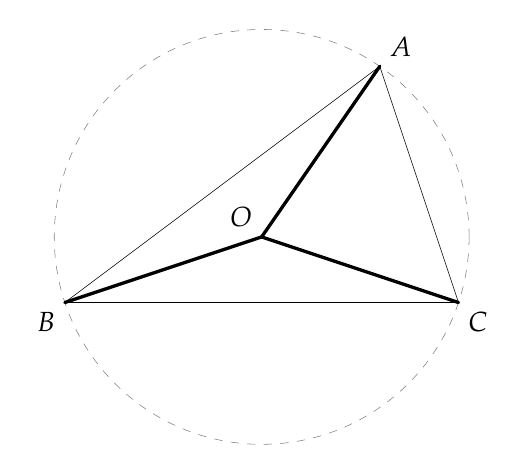
\begin{tikzpicture}
                \tkzDefPoint(4,3){A}
                \tkzDefPoint(0,0){B}
                \tkzDefPoint(5,0){C}
                \tkzDrawSegments(A,B B,C C,A)
            
                \tkzCircumCenter(A,B,C)\tkzGetPoint{O}
                \tkzDrawCircle[dashed](O,A)

                \tkzLabelPoints[above right](A)
                \tkzLabelPoints[below left](B)
                \tkzLabelPoints[below right](C)
                \tkzLabelPoints[above left](O)

                \tkzDrawSegments[very thick](A,O B,O C,O);
            \end{tikzpicture}
            \caption{三角形的外心}
        \end{center}
    \end{figure}\\
    由于点$ABC$均在圆上,且O为圆心:\vspace{5pt}
    \setcounter{equation}{0}
    \begin{align}
        &\left|\overrightarrow{OA}\right|=\left|\overrightarrow{OB}\right|=\left|\overrightarrow{OC}\right|\\[4mm]
        &\left|\overrightarrow{OA}\right|^2=\left|\overrightarrow{OB}\right|^2=\left|\overrightarrow{OC}\right|^2\\[4mm]
        &~\overrightarrow{OA}~^2=\overrightarrow{OB}~^2=\overrightarrow{OC}~^2
    \end{align}\\
    三角形外心的向量表达:
    \begin{large}
        \begin{equation*}
            ~\overrightarrow{OA}~^2=\overrightarrow{OB}~^2=\overrightarrow{OC}~^2
        \end{equation*}
    \end{large}

\newpage

\subsection{三角形重心的向量表达}
    三角形的重心是三条\textbf{中线}的交点。\\[3mm]
    设$BC$的中点为$D$,延长$GD$至$E$,使得$OD=ED$,连接$BE$,连接$CE$。
    \begin{figure}[h]
        \begin{center}
            \hspace{30pt}
            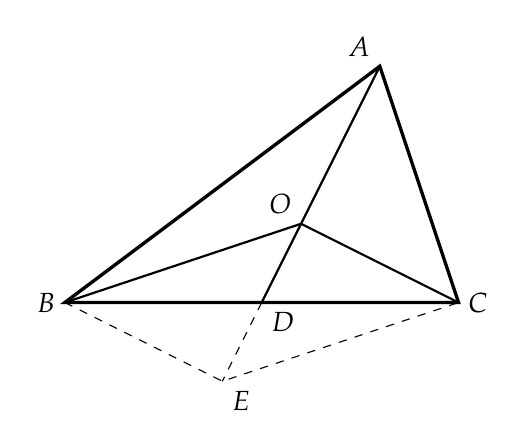
\begin{tikzpicture}
                \coordinate (A) at (4,3);
                \coordinate (B) at (0,0);
                \coordinate (C) at (5,0);
                \coordinate (O) at (3,1);
                \coordinate (D) at (2.5,0);
                \coordinate (E) at (2,-1);

                \node[above left] at(A) {$A$};
                \node[left] at(B) {$B$};
                \node[right] at(C) {$C$};
                \node[above left] at(O) {$O$};
                \node[below right] at(D) {$D$};
                \node[below right] at(E) {$E$};

                \draw[very thick](A)--(B)--(C)--cycle;
                \draw[thick] (A)--(O)--(D) (B)--(O) (C)--(O);
                \draw[dashed] (B)--(E)--(C) (D)--(E);
            \end{tikzpicture}
            \caption{三角形的重心}
        \end{center}
    \end{figure}\\
    显然我们有以下平行关系:
    \setcounter{equation}{0}
    \begin{align}
        OB\parallel CE\qquad OC\parallel BE
    \end{align}\\
    由此可以得到:
    \begin{align}
        \overrightarrow{OB}+\overrightarrow{OC}=\overrightarrow{OB}+\overrightarrow{BE}=\overrightarrow{OE}
    \end{align}\\
    根据重心的性质和平行关系:
    \begin{align}
        &\overrightarrow{OA}=2\overrightarrow{DO}\qquad\overrightarrow{OE}=2\overrightarrow{OD}\\[3mm]
        &\overrightarrow{OA}+\overrightarrow{OE}=2\overrightarrow{DO}-2\overrightarrow{OD}=\vec{0}
    \end{align}\\
    将向量$\overrightarrow{OE}$用$\overrightarrow{OE}=\overrightarrow{OB}+\overrightarrow{OC}$代换:
    \begin{align}
        \overrightarrow{OA}+\overrightarrow{OB}+\overrightarrow{OC}=\vec{0}
    \end{align}\\
    三角形重心的向量表达:
    \begin{large}
        \begin{equation*}
            ~\overrightarrow{OA}+\overrightarrow{OB}+\overrightarrow{OC}=\vec{0}
        \end{equation*}
    \end{large}

\newpage

\subsection{三角形垂心的向量表达}
    三角形的垂心是三条\textbf{垂线}的交点。\\[3mm]
    将点$A$垂线的垂足记为点$D$,将点$B$垂线的垂足记为点$E$,将点$C$垂线的垂足记为点$F$。
    \begin{figure}[h]
        \begin{center}
            \hspace{10pt}
            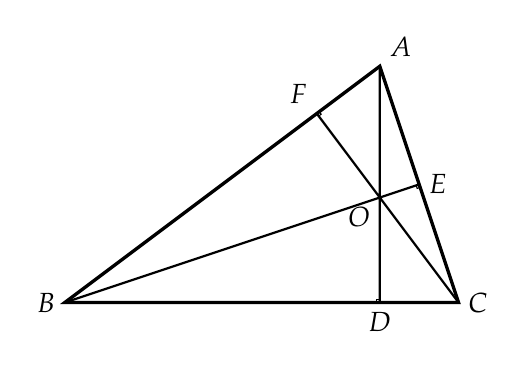
\begin{tikzpicture}
                \coordinate (A) at (4,3);
                \coordinate (B) at (0,0);
                \coordinate (C) at (5,0);
                \coordinate (D) at ($(C)!(A)!(B)$);
                \coordinate (F) at ($(B)!(C)!(A)$);
                \coordinate (E) at ($(A)!(B)!(C)$);
            
                \path[name path=AD] (A) -- (D);
                \path[name path=BE] (B) -- (E);
                \path[name intersections={of= AD and BE}];
                \coordinate (O) at (intersection-1);
            
                \node[above right] at(A) {$A$};
                \node[left] at(B) {$B$};
                \node[right] at(C) {$C$};
                \node[below] at(D) {$D$};
                \node[right] at(E) {$E$};
                \node[above left] at(F) {$F$};
                \node[below left] at(O) {$O$};
            
                \draw[very thick](A)--(B)--(C)--cycle;
                \draw[thick] (A)--(O)--(D) (B)--(O)--(E) (C)--(O)--(F);
            
                \tkzMarkRightAngle[scale=0.4](A,D,B);
                \tkzMarkRightAngle[scale=0.4](B,E,C);
                \tkzMarkRightAngle[scale=0.4](C,F,A);
            \end{tikzpicture}
            \caption{三角形的垂心}
        \end{center}
    \end{figure}\\
    由于$AD\perp BC$,根据向量的垂直条件:\vspace{5pt}
    \setcounter{equation}{0}
    \begin{align}
        &\overrightarrow{OA}\cdot\overrightarrow{BC}=\vec{0}\\[3mm]
        &\overrightarrow{OA}\cdot\left(\overrightarrow{OC}-\overrightarrow{OB}\right)=\vec{0}\\[3mm]
        &\overrightarrow{OA}\cdot\overrightarrow{OC}-\overrightarrow{OA}\cdot\overrightarrow{OB}=\vec{0}\\[3mm]
        &\overrightarrow{OA}\cdot\overrightarrow{OC}=\overrightarrow{OA}\cdot\overrightarrow{OB}
    \end{align}\\
    由于$CE\perp AB$,根据向量的垂直条件:\vspace{5pt}
    \begin{align}
        &\overrightarrow{OC}\cdot\overrightarrow{AB}=\vec{0}\\[3mm]
        &\overrightarrow{OC}\cdot\left(\overrightarrow{OA}-\overrightarrow{OB}\right)=\vec{0}\\[3mm]
        &\overrightarrow{OC}\cdot\overrightarrow{OA}-\overrightarrow{OC}\cdot\overrightarrow{OB}=\vec{0}\\[3mm]
        &\overrightarrow{OC}\cdot\overrightarrow{OA}=\overrightarrow{OC}\cdot\overrightarrow{OB}
    \end{align}\\
    三角形垂心的向量表达:
    \begin{large}
        \begin{equation*}
            \overrightarrow{OA}\cdot\overrightarrow{OB}=\overrightarrow{OB}\cdot\overrightarrow{OC}=\overrightarrow{OC}\cdot\overrightarrow{OA}
        \end{equation*}
    \end{large}

\newpage

\subsection{三角形垂心的向量表达}
    三角形的垂心是三条\textbf{垂线}的交点。\\[3mm]
    将点$A$垂线的垂足记为点$D$,将点$B$垂线的垂足记为点$E$,将点$C$垂线的垂足记为点$F$。
    \begin{figure}[h]
        \begin{center}
            \hspace{10pt}
            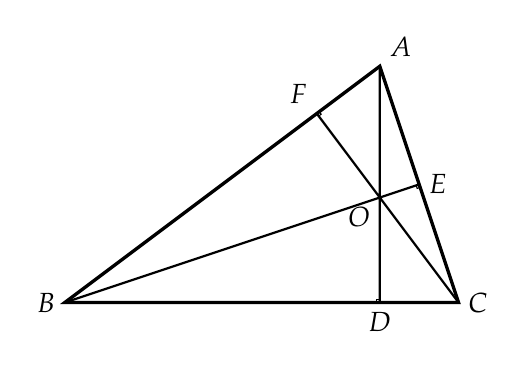
\begin{tikzpicture}
                \coordinate (A) at (4,3);
                \coordinate (B) at (0,0);
                \coordinate (C) at (5,0);
                \coordinate (D) at ($(C)!(A)!(B)$);
                \coordinate (F) at ($(B)!(C)!(A)$);
                \coordinate (E) at ($(A)!(B)!(C)$);
            
                \path[name path=AD] (A) -- (D);
                \path[name path=BE] (B) -- (E);
                \path[name intersections={of= AD and BE}];
                \coordinate (O) at (intersection-1);
            
                \node[above right] at(A) {$A$};
                \node[left] at(B) {$B$};
                \node[right] at(C) {$C$};
                \node[below] at(D) {$D$};
                \node[right] at(E) {$E$};
                \node[above left] at(F) {$F$};
                \node[below left] at(O) {$O$};
            
                \draw[very thick](A)--(B)--(C)--cycle;
                \draw[thick] (A)--(O)--(D) (B)--(O)--(E) (C)--(O)--(F);
            
                \tkzMarkRightAngle[scale=0.4](A,D,B);
                \tkzMarkRightAngle[scale=0.4](B,E,C);
                \tkzMarkRightAngle[scale=0.4](C,F,A);
            \end{tikzpicture}
            \caption{三角形的垂心}
        \end{center}
    \end{figure}\\
    由于$AD\perp BC$,根据向量的垂直条件:\vspace{5pt}
    \setcounter{equation}{0}
    \begin{align}
        &\overrightarrow{OA}\cdot\overrightarrow{BC}=\vec{0}\\[3mm]
        &\overrightarrow{OA}\cdot\left(\overrightarrow{OC}-\overrightarrow{OB}\right)=\vec{0}\\[3mm]
        &\overrightarrow{OA}\cdot\overrightarrow{OC}-\overrightarrow{OA}\cdot\overrightarrow{OB}=\vec{0}\\[3mm]
        &\overrightarrow{OA}\cdot\overrightarrow{OC}=\overrightarrow{OA}\cdot\overrightarrow{OB}
    \end{align}\\
    由于$CE\perp AB$,根据向量的垂直条件:\vspace{5pt}
    \begin{align}
        &\overrightarrow{OC}\cdot\overrightarrow{AB}=\vec{0}\\[3mm]
        &\overrightarrow{OC}\cdot\left(\overrightarrow{OA}-\overrightarrow{OB}\right)=\vec{0}\\[3mm]
        &\overrightarrow{OC}\cdot\overrightarrow{OA}-\overrightarrow{OC}\cdot\overrightarrow{OB}=\vec{0}\\[3mm]
        &\overrightarrow{OC}\cdot\overrightarrow{OA}=\overrightarrow{OC}\cdot\overrightarrow{OB}
    \end{align}\\
    三角形垂心的向量表达:
    \begin{large}
        \begin{equation*}
            \overrightarrow{OA}\cdot\overrightarrow{OB}=\overrightarrow{OB}\cdot\overrightarrow{OC}=\overrightarrow{OC}\cdot\overrightarrow{OA}
        \end{equation*}
    \end{large}

\newpage

\subsection{三角形的内心的向量表达}
    三角形的内心是三条\textbf{角平分线}的交点。\\[3mm]
    三角形的内心同时也是三角形内接圆的圆心。\\[3mm]
    设$BO$与$AC$相交于$E$,设$CO$与$AB$相交于$F$。\\[2mm]
    过$A$作$CO$的平行线,与$BO$的延长线相交于$N$。\\[2mm]
    过$A$作$BO$的平行线,与$CO$的延长线相交于$M$。
    \begin{figure}[htbp]
        \begin{center}
            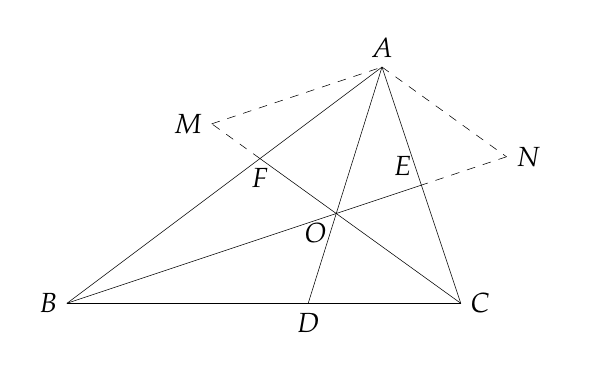
\begin{tikzpicture}
                \tkzInit[xmin=-0.5,xmax=6.5,ymin=-0.5,ymax=3.5]
                \tkzClip
                \tkzDefPoint(4,3){A}
                \tkzDefPoint(0,0){B}
                \tkzDefPoint(5,0){C}
                \tkzLabelPoints[above](A)
                \tkzLabelPoints[left](B)
                \tkzLabelPoints[right](C)
                \tkzDrawSegments(A,B B,C C,A)
            
                \tkzDefCircle[in](A,B,C)
                \tkzGetPoint{O}
                \tkzLabelPoints[below left](O)
            
                \tkzInterLL(A,O)(B,C)
                \tkzGetPoint{D}
                \tkzInterLL(B,O)(A,C)
                \tkzGetPoint{E}
                \tkzInterLL(C,O)(A,B)
                \tkzGetPoint{F}
                \tkzLabelPoints[below](D)
                \tkzLabelPoints[above left](E)
                \tkzLabelPoints[below](F)
                \tkzDrawSegments(A,D B,E C,F)
            
                \tkzDefLine[parallel=through A](B,O) 
                \tkzGetPoint{b}
                \tkzInterLL(A,b)(C,O)
                \tkzGetPoint{M}
                \tkzDefLine[parallel=through A](C,O) 
                \tkzGetPoint{c}
                \tkzInterLL(A,c)(B,O)
                \tkzGetPoint{N}
                \tkzLabelPoints[left](M)
                \tkzLabelPoints[right](N)
                \tkzDrawSegments[dashed](F,M M,A A,N N,E)
            \end{tikzpicture}
            \caption{三角形的内心}
        \end{center}
    \end{figure}\\
    根据内心的性质,内心到边$a$和边$b$的距离相等:\vspace{3pt}
    \setcounter{equation}{0}
    \begin{align}
        &\frac{b}{a}=\frac{AC}{BC}=\frac{S_{\triangle AOC}}{S_{\triangle BOC}}
    \end{align}\\
    根据$OC$和$OF$的比例可以得到:
    \begin{align}
        &\frac{OC}{OF}=\frac{S_{\triangle AOC}}{S_{\triangle AOF}}=\frac{S_{\triangle BOC}}{S_{\triangle BOF}}
    \end{align}\\
    进一步变形可得:
    \begin{align}
        &\frac{S_{\triangle AOC}}{S_{\triangle AOF}}=\frac{S_{\triangle BOC}}{S_{\triangle BOF}}\\[3mm]
        &\frac{S_{\triangle AOC}}{S_{\triangle BOC}}=\frac{S_{\triangle AOF}}{S_{\triangle BOF}}\\[3mm]
        &\frac{S_{\triangle AOC}}{S_{\triangle BOC}}=\frac{AF}{BF}
    \end{align}\\
    将面积代换最终得到:
    \begin{align}
        &\frac{b}{a}=\frac{AF}{BF}
    \end{align}
    
\newpage

    根据内心的性质,内心到边$a$和边$c$的距离相等:\vspace{3pt}
    \begin{align}
        &\frac{c}{a}=\frac{AB}{CB}=\frac{S_{\triangle AOB}}{S_{\triangle COB}}
    \end{align}\\
    根据$OB$和$OE$的比例可以得到:
    \begin{align}
        &\frac{OB}{OE}=\frac{S_{\triangle AOB}}{S_{\triangle AOE}}=\frac{S_{\triangle COB}}{S_{\triangle COE}}
    \end{align}\\
    进一步变形可得:
    \begin{align}
        &\frac{S_{\triangle AOB}}{S_{\triangle AOE}}=\frac{S_{\triangle COB}}{S_{\triangle COE}}\\[3mm]
        &\frac{S_{\triangle AOB}}{S_{\triangle COB}}=\frac{S_{\triangle AOE}}{S_{\triangle COE}}\\[3mm]
        &\frac{S_{\triangle AOB}}{S_{\triangle COB}}=\frac{AE}{CE}
    \end{align}\\
    将面积代换最终得到:
    \begin{align}
        &\frac{c}{a}=\frac{AE}{CE}
    \end{align}\\
    由于$AM\parallel ON$且$AN\parallel OM$,所以四边形$AMON$是一个平行四边形:
    \begin{align}
        \overrightarrow{OA}
        &=\overrightarrow{OM}+\overrightarrow{ON}\\[3mm]
        &=\left(\frac{OM}{CO}\right)\cdot\overrightarrow{CO}+\frac{ON}{BO}\cdot\overrightarrow{BO}\\[3mm]
        &=\left(\frac{AN}{CO}\right)\cdot\overrightarrow{CO}+\frac{AM}{BO}\cdot\overrightarrow{BO}
    \end{align}\\
    因为$AN\parallel CO$且$AM\parallel BO$:
    \begin{align}
        &\frac{AN}{CO}=\frac{AE}{CE}=\frac{c}{a}\qquad\frac{AM}{BO}=\frac{AF}{BF}=\frac{b}{a}
    \end{align}\\
    最终代入可得:
    \begin{align}
        &\overrightarrow{OA}=\frac{c}{a}\cdot\overrightarrow{CO}+\frac{b}{a}\cdot\overrightarrow{BO}\\[3mm]
        &a\cdot\overrightarrow{OA}=c\cdot\overrightarrow{CO}+b\cdot\overrightarrow{BO}
    \end{align}\\
    三角形内心的向量表达:
    \begin{large}
        \begin{equation*}
            a\cdot\overrightarrow{OA}+b\cdot\overrightarrow{OB}+c\cdot\overrightarrow{OC}=\vec{0}
        \end{equation*}
    \end{large}


\newpage

\section{矩阵}
    我们将一个由$m$行$n$列组成的矩形数表称为矩阵:\\
    \begin{large}
    \begin{equation*}
        A=
        \begin{pmatrix}
            a_{1,1}&a_{1,2}&\cdots&a_{1,n}\\
            a_{2,1}&a_{2,2}&\cdots&a_{2,n}\\
            \vdots&\vdots&\ddots&\vdots\\
            a_{m,1}&a_{m,2}&\cdots&a_{m,n}
        \end{pmatrix}
    \end{equation*}
    \end{large}

\subsection{矩阵的加法和减法}
    对于矩阵:
    \begin{large}
    \begin{equation*}
        A=
        \begin{pmatrix}
            a_{1,1}&a_{1,2}\\
            a_{2,1}&a_{2,2}
        \end{pmatrix}\qquad
        B=
        \begin{pmatrix}
            b_{1,1}&b_{1,2}\\
            b_{2,1}&b_{2,2}
        \end{pmatrix}\qquad
    \end{equation*}
    \end{large}\\
    矩阵的加法:
    \begin{large}
    \begin{equation*}
        A+B=
        \begin{pmatrix}
            a_{1,1}+b_{1,1}&a_{1,2}+b_{1,2}\\
            a_{2,1}+b_{2,1}&a_{2,2}+b_{2,2}
        \end{pmatrix}
    \end{equation*}
    \end{large}\\
    矩阵的减法:
    \begin{large}
    \begin{equation*}
        A-B=
        \begin{pmatrix}
            a_{1,1}-b_{1,1}&a_{1,2}-b_{1,2}\\
            a_{2,1}-b_{2,1}&a_{2,2}-b_{2,2}
        \end{pmatrix}
    \end{equation*}
    \end{large}\\
    请注意,只有对于同型的矩阵才可以进行加减运算!\\[6mm]
    矩阵的加法满足加法交换律:
    \begin{large}
    \begin{equation*}
        A+B=B+A
    \end{equation*}
    \end{large}\\
    矩阵的加法满足加法结合律:
    \begin{large}
    \begin{equation*}
        A+(B+C)=(A+B)+C
    \end{equation*}
    \end{large}

\newpage

\subsection{矩阵的数乘}
    对于矩阵:
    \begin{large}
    \begin{equation*}
        A=
        \begin{pmatrix}
            a_{1,1}&a_{1,2}\\
            a_{2,1}&a_{2,2}
        \end{pmatrix}
    \end{equation*}
    \end{large}\\
    矩阵的数乘:
    \begin{large}
    \begin{equation*}
        c\cdot A=
        \begin{pmatrix}
            c\cdot a_{1,1}&c\cdot a_{1,2}\\
            c\cdot a_{2,1}&c\cdot a_{2,2}
        \end{pmatrix}
    \end{equation*}
    \end{large}\\
    矩阵的数乘满足乘法交换律:
    \begin{large}
    \begin{equation*}
        c\cdot A=A\cdot c
    \end{equation*}
    \end{large}\\
    矩阵的数乘满足乘法结合律:
    \begin{large}
    \begin{equation*}
        c\cdot d \cdot A=c\cdot (d\cdot A)=d\cdot (c\cdot A)
    \end{equation*}
    \end{large}\\
    矩阵的数乘满足乘法分配律:
    \begin{large}
    \begin{equation*}
        (c+d)\cdot A=c\cdot A+d\cdot A
    \end{equation*}
    \begin{equation*}
        c\cdot(A+B)=c\cdot A+c\cdot B    
    \end{equation*}
    \end{large}

\newpage

\subsection{矩阵的乘法}
    对于矩阵:
    \begin{large}
        \begin{equation*}
            A=\left(a_{ma,na}\right)\qquad
            B=\left(b_{mb,nb}\right)\qquad
        \end{equation*}
    \end{large}\\
    当矩阵$A$的列数与矩阵$B$的行数相等,即$na=mb$时,我们定义:
    \begin{large}
        \begin{equation*}
            A\cdot B=C
        \end{equation*}
    \end{large}\\
    \textbf{对于矩阵$C$的行数和列数:}
    \begin{large}
        \begin{equation*}
            C=\left(c_{ma,nb}\right)
        \end{equation*}
    \end{large}\\
    即行数为矩阵$A$的行数,列数为矩阵$B$的列数。(行看$A$,列看$B$)\\[10mm]
    \textbf{对于矩阵$C$的值(其中$r=na=mb$):}
    \begin{large}
        \begin{equation*}
            c_{i,j}=\sum_{x=1}^{r}a_{i,x}\cdot b_{x,j}
        \end{equation*}
    \end{large}
    即$c_{i,j}$等于矩阵A的第$i$个行向量和第$j$个列向量的内积。($A$的第$i$行乘以$B$的第$j$列)\\[10mm]
    矩阵的乘法\textbf{不满足}乘法交换律!\\[3mm]
    矩阵的乘法满足乘法结合律:
    \begin{large}
        \begin{equation*}
            A\cdot B\cdot C=(A\cdot B)\cdot C=A\cdot(B\cdot C)    
        \end{equation*}
    \end{large}
    矩阵的乘法满足乘法分配律:
    \begin{large}
        \begin{equation*}
            (A+B)\cdot C=A\cdot C+B\cdot C
        \end{equation*}
        \begin{equation*}
            C\cdot (A+B)=C\cdot A+C\cdot B
        \end{equation*}
    \end{large}

\newpage

\subsection{矩阵的转置}
    我们将原矩阵的行和列互换所产生的矩阵称为转置矩阵,这一过程称为转置。\\[3mm]
    矩阵$A$的转置矩阵记作$A^T$。\\[6mm]
    考虑以下例子:
    \begin{large}
        \begin{equation*}
            \begin{pmatrix}
                1&2&3\\
                4&5&6
            \end{pmatrix}^T=
            \begin{pmatrix}
                1&4\\
                2&5\\
                3&6
            \end{pmatrix}
        \end{equation*}\\
        \begin{equation*}
            \begin{pmatrix}
                1&2&3\\
                4&5&6\\
                7&8&9
            \end{pmatrix}^T=
            \begin{pmatrix}
                1&4&7\\
                2&5&8\\
                3&6&9
            \end{pmatrix}
        \end{equation*}
    \end{large}\\[3mm]
    除了行列的互换,我们还可以将转置理解为矩阵关于主对角线的翻折。\\[6mm]
    矩阵的转置满足以下运算规律:
    \begin{large}
        \begin{align*}
            &(A^T)^T=A\\[4mm]
            &(c\cdot A)^T=c\cdot A^T\\[4mm]
            &(AB)^T=B^T\cdot A^T\\[4mm]
        \end{align*}
    \end{large}

\newpage

\section{行列式}
    行列式是一个由$n\times n$个数组成的特定运算的符号,本质是一个数:
    \begin{large}
        \begin{equation*}
            D=
            \begin{vmatrix}
                a_{1,1}&a_{1,2}&\cdots&a_{1,n}\\
                a_{2,1}&a_{2,2}&\cdots&a_{2,n}\\
                \vdots&\vdots&\ddots&\vdots\\
                a_{m,1}&a_{m,2}&\cdots&a_{m,n}
            \end{vmatrix}
        \end{equation*}
    \end{large}\\
    我们将一个由$n$行$n$列组成的行列式称为$n$阶行列式。

\subsection{二阶行列式}
    二阶行列式的运算法则:
    \begin{large}
        \begin{equation*}
            D=
            \begin{vmatrix}
                a_1&b_1\\
                a_2&b_2\\
            \end{vmatrix}
            =a_1b_2-a_2b_1
        \end{equation*}
    \end{large}

\subsubsection{二元一次方程组的行列式解法}
    对于二元一次方程组:
    \begin{large}
        \begin{equation*}
            \begin{cases}
                \ a_{1}\cdot x+b_{1}\cdot y=c_{1}\\
                \ a_{2}\cdot x+b_{2}\cdot y=c_{2}\\
            \end{cases}
        \end{equation*}
    \end{large}\\
    我们定义行列式$D$:
    \begin{large}
        \begin{equation*}
            D=
            \begin{vmatrix}
                a_1&b_1\\
                a_2&b_2\\
            \end{vmatrix}
        \end{equation*}
    \end{large}\\
    使用常数项$c$所在的一列替换$x$的参数$a$所在的一列,得到行列式$D_x$:
    \begin{large}
        \begin{equation*}
            D_x=
            \begin{vmatrix}
                c_1&b_1\\
                c_2&b_2\\
            \end{vmatrix}
        \end{equation*}
    \end{large}\\
    使用常数项$c$所在的一列替换$y$的参数$b$所在的一列,得到行列式$D_y$:
    \begin{large}
        \begin{equation*}
            D_y=
            \begin{vmatrix}
                a_1&c_1\\
                a_2&c_2\\
            \end{vmatrix}
        \end{equation*}
    \end{large}

\newpage

    当$D\neq 0$时,我们可以得到方程组的解:
    \begin{large}
        \begin{equation*}
            \begin{cases}
                \ x=\dfrac{D_x}{D} \\[6mm]
                \ y=\dfrac{D_y}{D} \\
            \end{cases}
        \end{equation*}
    \end{large}\\
    当$D=0$时,若$D_x\neq 0$或$D_y\neq 0$,方程组无解。\\[3mm]
    当$D=0$时,若$D_x=0$且$D_y=0$,方程组有无穷多解。\\

\subsection{三阶行列式}
    三阶行列式的运算法则:\vspace{5pt}
    \begin{large}
        \begin{equation*}
            D=
            \begin{vmatrix}
                a_1&b_1&c_1\\
                a_2&b_2&c_2\\
                a_3&b_3&c_3\\
            \end{vmatrix}
            =a_1b_2c_3+a_2b_3c_1+a_3b_1c_2
            -a_3b_2c_1-a_2b_1c_3-a_1b_3c_2
        \end{equation*}
    \end{large}

\subsubsection{三元一次方程组的行列式解法}
    对于三元一次方程组:
    \begin{large}
        \begin{equation*}
            \begin{cases}
                \ a_{1}\cdot x+b_{1}\cdot y+c_{1}\cdot z=d_{1}\\
                \ a_{2}\cdot x+b_{2}\cdot y+c_{2}\cdot z=d_{2}\\
                \ a_{3}\cdot x+b_{3}\cdot y+c_{3}\cdot z=d_{3}\\
            \end{cases}
        \end{equation*}
    \end{large}\\
    我们定义系数行列式$D$:
    \begin{large}
        \begin{equation*}
            D=
            \begin{vmatrix}
                a_1&b_1&c_1\\
                a_2&b_2&c_2\\
                a_3&b_3&c_3\\
            \end{vmatrix}
        \end{equation*}
    \end{large}\\[2mm]
    使用常数项$d$所在的一列替换$x$的参数$a$所在的一列,得到行列式$D_x$:
    \begin{large}
        \begin{equation*}
            D_x=
            \begin{vmatrix}
                d_1&b_1&c_1\\
                d_2&b_2&c_2\\
                d_3&b_3&c_3\\
            \end{vmatrix}
        \end{equation*}
    \end{large}

\newpage

    使用常数项$d$所在的一列替换$y$的参数$b$所在的一列,得到行列式$D_y$:
    \begin{large}
        \begin{equation*}
            D_y=
            \begin{vmatrix}
                a_1&d_1&c_1\\
                a_2&d_2&c_2\\
                a_3&d_3&c_3\\
            \end{vmatrix}
        \end{equation*}
    \end{large}\\
    使用常数项$d$所在的一列替换$z$的参数$c$所在的一列,得到行列式$D_z$:
    \begin{large}
        \begin{equation*}
            D_z=
            \begin{vmatrix}
                a_1&b_1&d_1\\
                a_2&b_2&d_2\\
                a_3&b_3&d_3\\
            \end{vmatrix}
        \end{equation*}
    \end{large}\\
    当$D\neq 0$时,我们可以得到方程组的解:
    \begin{large}
        \begin{equation*}
            \begin{cases}
                \ x=\dfrac{D_x}{D} \\[6mm]
                \ y=\dfrac{D_y}{D} \\[6mm]
                \ z=\dfrac{D_z}{D}
            \end{cases}
        \end{equation*}
    \end{large}\\
    当$D=0$时,方程组可能是无解或无穷多解,具体情况需要代入数字验证。\\

\subsection{利用行列式求解三角形面积}
    对于$\triangle ABC$,
    如果三角形的顶点坐标分别为$A(x_1,y_1)$,$B(x_2,y_2)$,$C(x_3,y_3)$。\\[3mm]
    三角形的面积公式:
    \begin{large}
        \begin{equation*}
            S_{\triangle ABC}=\frac{1}{2}\cdot
            \begin{vmatrix}
                x_1&y_1&1\\
                x_2&y_2&1\\
                x_3&y_3&1\\
            \end{vmatrix}
        \end{equation*}
    \end{large}\\
    需要注意的是:\\[3mm]
    如果顶点ABC按逆时针排列,行列式为正值。\\[3mm]
    如果顶点ABC按顺时针排列,行列式为负值。\\[3mm]

\newpage

\subsection{代数余子式}
    对于行列式$D$和该行列式中的一个元素$u$,
    我们将行列式$D$中划去元素$u$所在的行和列后,
    剩下的元素重新组成的行列式,称为元素$u$的余子式。
    在余子式的基础上添加元素所对应的符号,
    则称为代数余子式。\\[3mm]
    其中元素和符号的对应关系如下:
    \begin{large}
        \begin{equation*}
            \begin{vmatrix}
                +&-&+\\
                -&+&-\\
                +&-&+\\
            \end{vmatrix}
        \end{equation*}
    \end{large}\\
    代数余子式通常记作元素对应的大写字母并附加相同下标,例如$a_1$的代数余子式$A_1$。
    \subsubsection*{请考虑以下例子:}
    对于行列式:
    \begin{large}
        \begin{equation*}
            D=
            \begin{vmatrix}
                a_1&b_1&c_1\\
                a_2&b_2&c_2\\
                a_3&b_3&c_3\\
            \end{vmatrix}
        \end{equation*}
    \end{large}\\
    我们有代数余子式:\vspace{5pt}
    \begin{large}
        \begin{equation*}
            A_1=+
            \begin{vmatrix}
                b_2&c_2\\
                b_3&c_3\\
            \end{vmatrix}\qquad
            B_1=-
            \begin{vmatrix}
                a_2&c_2\\
                a_3&c_3\\
            \end{vmatrix}\qquad
            B_2=+
            \begin{vmatrix}
                a_1&c_1\\
                a_3&c_3\\
            \end{vmatrix}
        \end{equation*}
    \end{large}\\[2mm]
    行列式的值等于其任意一行或任意一列中元素与其对应代数余子式的乘积之和。\\

\newpage

\section{直线方程}

\subsection{点方向式方程}
    需要求解直线$l$的方程,已知直线过点$P$,
    且平行于向量$\vec d$,\\[1mm]
    此时我们适合使用点方向式方程表示这条直线。\\[3mm]
    我们已知:
    \begin{large}
        \begin{equation*}
            P(x_{0},y_{0})\qquad
            \vec d = (u,v)
        \end{equation*}
    \end{large}\\
    对于直线$l$上任意一点$Q(x,y)$,
    我们可以求得向量$\overrightarrow{PQ}=(x-x_0,y-y_0)$,
    由于向量$\overrightarrow{PQ}\parallel \vec{d}$,
    根据向量的平行公式,我们可以建立方程。\\[3mm]
    点方向式方程:
    \begin{large}
        \begin{equation*}
            v\cdot(x-x_{0})-u\cdot(y-y_0)=0
        \end{equation*}
    \end{large}\\
    其中,平行于直线$l$的向量$\vec d$被称为方向向量(direction vector)。\\[5mm]
    为了更加方便的构造方程,
    点方向式方程还有以下两种孪生形式:\\[3mm]
    1.通过点$P(x_0,y_0)$和方向向量$\vec{d}=(u,v)$构造方程:
    \vspace{5pt}
    \begin{large}
        \begin{equation*}
            \frac{x-x_0}{u}=\frac{y-y_0}{v}
        \end{equation*}
    \end{large}\\
    2.通过点$P(x_1,y_1)$和点$Q(x_2,y_2)$构造方程:
    \vspace{5pt}
    \begin{large}
        \begin{equation*}
            \frac{x-x_1}{x_1-x_2}=\frac{y-y_1}{y_1-y_2}
        \end{equation*}
    \end{large}\\[1mm]
    这两种形式虽然可以更加快速的构建方程,
    但由于需要讨论分母是否为0,
    所以在解决复杂问题时并不好用,
    但数学教材仍然将上述的第一种形式作为点方向式的定义。

\newpage

\subsection{点法向式方程}
    需要求解直线$l$的方程,已知直线过点$P$,
    且垂直于向量$\vec n$,\\[1mm]
    此时我们适合使用点法向式方程表示这条直线。\\[3mm]
    我们已知:
    \begin{large}
        \begin{equation*}
            P(x_{0},y_{0})\qquad
            \vec n = (u,v)
        \end{equation*}
    \end{large}\\
    对于直线$l$上任意一点$Q(x,y)$,
    我们可以求得向量$\overrightarrow{PQ}=(x-x_0,y-y_0)$,
    由于向量$\overrightarrow{PQ}\perp\vec{n}$,
    根据向量的垂直公式,我们可以建立方程。\\[3mm]
    点法向式方程:
    \begin{large}
        \begin{equation*}
            u \cdot (x-x_{0})+v \cdot (y-y_{0}) = 0
        \end{equation*}
    \end{large}\\
    其中,垂直于直线$l$的向量$\vec n$被称为法向量(normal vector)。\\

\subsection{点斜式方程}
    对于一次函数,我们学习过斜率$k$的概念,
    斜率(slope)代表了直线的陡峭程度。\\[3mm]
    直线$l$与$x$轴间的最小正角称为直线l的倾斜角,
    倾斜角$\alpha$的取值范围$[\ 0,\pi\ )$\\[6mm]
    当$\alpha \neq \dfrac{\pi}{2}$时,
    $k = \tan \alpha$\\[3mm]
    当$\alpha = \dfrac{\pi}{2}$时,
    $k$不存在\\[6mm]
    当$k<0$时,
    $\alpha=\arctan{(k)}+\pi$\\[3mm]
    当$k>0$时,
    $\alpha=\arctan{(k)}$\\[3mm]
    当$k=0$时,
    $\alpha=0$\\[6mm]
    需要求解直线$l$的方程,已知过点$P(x_{0},y_{0})$,
    且已知直线与$x$轴的夹角$\alpha$,
    或已知直线的斜率$k$,
    此时我们适合使用点斜式方程表示这条直线。\\[3mm]
    点斜式方程:
    \begin{large}
        \begin{equation*}
            y-y_{0} = (x-x_{0}) \cdot \tan \alpha
        \end{equation*}
        \begin{equation*}
            y-y_{0} = (x-x_{0}) \cdot k
        \end{equation*}
    \end{large}

\newpage

\subsection{截距式方程}
    如果我们已知直线$l$在$x$轴及$y$轴上的截距,
    那么此时适合用截距式方程表示这条直线。\\[3mm]
    我们已知直线在$x$轴上的截距为$a$,在$y$轴上的截距为$b$,
    显然这条直线过点$A(a,0)$,点$B(0,b)$,
    代入点方向式方程的第二种孪生形式:
    \vspace{5pt}
    \setcounter{equation}{0}
    \begin{align}
        &\frac{x-a}{a-0}=\frac{y-0}{0-b}\\[4mm]
        &\frac{x-a}{a}=-\frac{y}{b}\\[4mm]
        &\frac{x-a}{a}+\frac{y}{b}=0\\[4mm]
        &\frac{x}{a}+\frac{y}{b}-\frac{a}{a}=0\\[4mm]
        &\frac{x}{a}+\frac{y}{b}-1=0
    \end{align}\\
    截距式方程:
    \begin{large}
        \begin{equation*}
            \frac{x}{a}+\frac{y}{b}=1
        \end{equation*}
    \end{large}\\

\subsection{斜截式方程}
    如果我们已知直线$l$的斜率$k$和在y轴上的截距$b$,
    我们可以直接使用初中所学过的一次函数的形式表达这条直线,
    这种形式在直线方程中被称为斜截式方程。\\[3mm]
    由于直线方程中$x$和$y$间的关系是平等的,所以我们可以调换$x$和$y$的位置,得到另一种形式。\\[3mm]
    斜截式方程1:
    \begin{large}
        \begin{equation*}
            y=kx+b
        \end{equation*}
    \end{large}\\
    斜截式方程2:
    \begin{large}
        \begin{equation*}
            x=ty+b
        \end{equation*}
    \end{large}\\
    对于第一种情况,参数$b$代表直线在$y$轴上的截距。\\[2mm]
    对于第二种情况,参数$b$代表直线在$x$轴上的截距。\\[2mm]


\newpage

\subsection{一般式方程}
    直线方程的各种形式实际上
    均可以化为关于$x$,$y$的二元一次方程。\\[3mm]
    我们称这种形式为直线的一般式方程:
    \begin{large}
        \begin{equation*}
            ax+by+c=0
        \end{equation*}
    \end{large}\\
    对于直线方程$l:ax+by+c=0$:\\[6mm]
    直线$l$的方向向量:
    \begin{large}
        \begin{equation*}
            \vec{d}= (-b,a)\qquad\vec{d}=(b,-a)
        \end{equation*}
    \end{large}\\[1mm]
    直线$l$的法向量:
    \begin{large}
        \begin{equation*}
            \vec{n}= (a,b)\qquad\vec{n}=(-a,-b)
        \end{equation*}
    \end{large}\\[1mm]
    直线$l$的斜率:
    \begin{large}
        \begin{equation*}
            k = -\dfrac{a}{b}
        \end{equation*}
    \end{large}\\[1mm]
    直线$l$经过点:
    \begin{large}
        \begin{equation*}
            A(0,-\dfrac{c}{b})\qquad B(-\dfrac{c}{a},0)
        \end{equation*}
    \end{large}

\newpage

\subsection{两条直线的关系}
    我们设两条直线的方程为:
    \begin{align*}
        l_{1}&:a_{1}x+b_{1}y+c_{1}=0\\
        l_{2}&:a_{2}x+b_{2}y+c_{2}=0
    \end{align*}\\
    联立方程,可以得到方程组:\\
    \begin{equation*}
        \begin{cases}
            \ a_{1}x+b_{1}y=-c_{1}\\
            \ a_{2}x+b_{2}y=-c_{2}
        \end{cases}
    \end{equation*}\\[4mm]
    如果方程组有一组解,代表两条直线相交,存在一个交点。\\[3mm]
    如果方程组无解,代表两条直线平行,没有交点。\\[3mm]
    如果方程组有无穷解,代表两条直线重合,存在无穷多个交点。\\[3mm]

    我们可以应用行列式来解方程组:\\
    \begin{equation*}
        D=
        \left|
        \begin{matrix}
            a_{1} & b_{1}\\
            a_{2} & b_{2}\\
        \end{matrix}
        \right|
        \qquad\qquad
        D_{x}=
        \left|
        \begin{matrix}
            -c_{1} & b_{1}\\
            -c_{2} & b_{2}\\
        \end{matrix}
        \right|
        \qquad\qquad
        D_{y}=
        \left|
        \begin{matrix}
            a_{1} & -c_{1}\\
            a_{2} & -c_{2}\\
        \end{matrix}
        \right|
    \end{equation*}\\[3mm]
    当$a_{1}b_{2} \neq a_{1}b_{2}$时,
    方程有唯一解,两条直线相交,
    交点$P(\dfrac{D_{x}}{D},\dfrac{D_{y}}{D})$\\[4mm]
    当$a_{1}b_{2} = a_{1}b_{2}$时,若$D_{x}\neq 0$或$D_{y}\neq 0$,方程无解,两条直线平行。\\[4mm]
    当$a_{1}b_{2} = a_{1}b_{2}$时,若$D_{x}=0$或$D_{y}=0$,方程有无穷解,两条直线重合。

\newpage

\subsection{两条直线的夹角}
    我们设两条直线的方程为:
    \begin{align*}
        l_{1}&:a_{1}x+b_{1}y+c_{1}=0\\
        l_{2}&:a_{2}x+b_{2}y+c_{2}=0
    \end{align*}\\
    两条直线的方向向量分别为
    $\vec d_{1} = (-b_{1},a_{1})\quad\vec d_{2} = (-b_{2},a_{2})$。\\[3mm]
    因为两条直线的夹角的取值范围为$[0,\dfrac{\pi}{2}]$,\\[3mm]
    所以两条直线的夹角公式应当是两条直线所对应的方向向量夹角的绝对值。\\[12mm]
    两条直线的夹角公式:
    \begin{large}
        \begin{equation*}
            \cos{\alpha}=\frac{\left|a_{1}a_{2}+b_{1}b_{2}\right|}{\sqrt{{a_{1}}^{2}+{b_{1}}^{2}}\cdot\sqrt{{a_{2}}^{2}+{b_{2}}^{2}}}
        \end{equation*}  
    \end{large}\\
    特别的,当$a_{1}a_{2}+b_{1}b_{2}=0$时,两条直线垂直。\\[12mm]
    由于$k_{1} \cdot k_{2} = \dfrac{a_{1}a_{2}}{b_{1}b_{2}} = \dfrac{a_{1}a_{2}+b_{1}b_{2}}{b_{1}b_{2}}-1$\\[6mm]
    所以当两条直线垂直时,斜率满足:
    \begin{large}
        \begin{equation*}
            k_{1} \cdot k_{2} = -1     
        \end{equation*}
    \end{large}

\newpage

\subsection{点在直线上的射影点}
    已知点$P(i,j)$和直线$l:ax+by+c=0$,
    求解点在直线上的射影点$H$。\\[3mm]
    首先构造直线$l_{PH}$的方程:
    \setcounter{equation}{0}
    \begin{equation}
        l_{PH}:-bx+ay+d=0
    \end{equation}\\
    由于点$P$在直线$l_{PH}$,代入可得:
    \begin{align}
        -b&i+aj+d=0\\[2mm]
        &d=bi-aj
    \end{align}\\
    从而得到$l_{PH}$的方程:
    \begin{equation}
        l_{PH}:-bx+ay+(bi-aj)=0
    \end{equation}\\
    联立直线$l$和直线$l_{PH}$,建立方程组:\vspace{5pt}
    \begin{align}
        &\begin{cases}
            \ ax+by+c=0\\
            \ -bx+ay+(bi-aj)=0
        \end{cases}\\[6mm]
        &\begin{cases}
            \ ax+by=-c\\
            \ -bx+ay=-(bi-aj)
        \end{cases}
    \end{align}\\
    通过行列式求解方程组:
    \begin{align}
        &D=a^2+b^2\\[3mm]
        &D_x=-ac+b\cdot(bi-aj)\\[3mm]
        &D_y=-bc-a\cdot(bi-aj)
    \end{align}\\
    射影点$H$的坐标:\vspace{5pt}
    \begin{large}
        \begin{equation*}
            H\left(\frac{-ac+b\cdot(bi-aj)}{a^2+b^2}~~,~~\frac{-bc-a\cdot(bi-aj)}{a^2+b^2}\right)
        \end{equation*}
    \end{large}

\newpage

\subsection{点关于直线的对称点}
    已知点$P(i,j)$和直线$l:ax+by+c=0$,
    求解点关于直线的对称点$Q$。\\[3mm]
    设点$P$在直线$l$上的射影点为$H$,显然我们有:
    \setcounter{equation}{0}
    \begin{align}
        \overrightarrow{OQ}
        &=\overrightarrow{OP}+\overrightarrow{PQ}\\[2mm]
        &=\overrightarrow{OP}+2\cdot\overrightarrow{PH}\\[2mm]
        &=\overrightarrow{OP}+2\cdot\left(\overrightarrow{OH}-\overrightarrow{OP}\right)\\[2mm]
        &=\overrightarrow{OP}+2\cdot\overrightarrow{OH}-2\cdot\overrightarrow{OP}\\[2mm]
        &=2\cdot\overrightarrow{OH}-\overrightarrow{OP}\\
        &=2\cdot\left(\frac{-ac+b\cdot(bi-aj)}{a^2+b^2}~~,~~\frac{-bc-a\cdot(bi-aj)}{a^2+b^2}\right)-(i,j)
    \end{align}\\
    对称点$Q$的坐标:\vspace{5pt}
    \begin{large}
        \begin{equation*}
            Q\left(2\cdot\frac{-ac+b\cdot(bi-aj)}{a^2+b^2}-i~~,~~2\cdot\frac{-bc-a\cdot(bi-aj)}{a^2+b^2}-j\right)
        \end{equation*}
    \end{large}

\newpage

\subsection{点到直线的距离}
    已知点$P(i,j)$和直线$l:ax+by+c=0$,
    求解点到直线的距离$d$。\\[3mm]
    设点$H$为$P$在直线$l$上的射影点,由于距离$d$等于线段$PH$的长度:\vspace{15pt}
    \setcounter{equation}{0}
    \begin{align}
        &d^2=\left[\frac{-ac+b\cdot(bi-aj)}{a^2+b^2}-i^2\right]^2+\left[\frac{-bc-a\cdot(bi-aj)}{a^2+b^2}-j^2\right]^2\\[7mm]
        &d^2=\left[\frac{-ac+b^2i-abj-a^2i-b^2i}{a^2+b^2}\right]^2+\left[\frac{-bc+a^2j-abi-a^2j-b^2j}{a^2+b^2}\right]^2\\[7mm]
        &d^2=\left[\frac{-ac-abj-a^2i}{a^2+b^2}\right]^2+\left[\frac{-bc-abi-b^2j}{a^2+b^2}\right]^2\\[7mm]
        &d^2=\frac{a^2\cdot\left(-c-bj-ai\right)^2}{\left(a^2+b^2\right)^2}+\frac{b^2\cdot\left(-c-ai-bj\right)^2}{\left(a^2+b^2\right)^2}\\[7mm]
        &d^2=\frac{(a^2+b^2)\cdot\left(-c-bj-ai\right)^2}{\left(a^2+b^2\right)^2}\\[7mm]
        &d^2=\frac{\left(-c-bj-ai\right)^2}{a^2+b^2}\\[8mm]
        &d=\frac{\left|ax_{0}+by_{0}+c\right|}{\sqrt{{a}^{2}+{b}^{2}}}
    \end{align}\\[1mm]
    点到直线的距离公式:
    \begin{large}
        \begin{equation*}
            d=\frac{\left|ax_{0}+by_{0}+c\right|}{\sqrt{{a}^{2}+{b}^{2}}}
        \end{equation*}
    \end{large}\\

\newpage

\subsection{两条平行线间的距离}
    对于两条平行的直线:
    \begin{align*}
        l_{1}:ax+by+c_{1}=0\\
        l_{2}:ax+by+c_{2}=0
    \end{align*}\\
    设点$P(u,v)$在直线$l_{1}:ax+by+c_{1}=0$上,代入可得:
    \begin{equation*}
        a \cdot u+b \cdot v=-c_{1}
    \end{equation*}\\
    根据两点之间距离公式,点$P$到直线$l_{2}$的距离为:\\
    \begin{equation*}
        d=\frac{\left|au+bv+c_{2}\right|}{\sqrt{a^2+b^2}}
        =\frac{\left|-c_{1}+c_{2}\right|}{\sqrt{a^2+b^2}}
        =\frac{\left|c_{1}-c_{2}\right|}{\sqrt{a^2+b^2}}
    \end{equation*}\\[4mm]
    两条平行线之间的距离公式:
    \begin{large}
        \begin{equation*}
            d=\frac{\left|c_{1}-c_{2}\right|}{\sqrt{a^2+b^2}}
        \end{equation*}
    \end{large}

\newpage

\section{圆锥曲线方程}

\subsection{圆的方程}
    圆的定义:
    平面内到一个定点的距离等于定长的点的轨迹称为圆。\\[1mm]
    其中定点称为圆心$O(a,b)$,定长称为半径$r$。\\[3mm]
    确定一个圆需要两个条件:圆的圆心和圆的半径。\\[3mm]
    根据圆的定义,
    圆的方程应当满足方程的所有解满足到
    圆心$O$的距离为半径$r$,
    通过两点间距离公式,我们可以得出圆的方程。\\[5mm]
    圆的方程:
    \begin{large}
        \begin{equation*}
            \sqrt{(x-a)^2+(y-b)^2}=r
        \end{equation*}
    \end{large}
    \begin{figure}[h]
        \begin{center}
            \begin{tikzpicture}[>=stealth,scale=1.1]
                \draw[->] (-5.6,0) -- (5.6,0) node[above] {$x$};
                \draw[->] (0,-5.6) -- (0,5.6) node[right] {$y$};
                \foreach \x in {-5,-4,...,-1}
                    \draw[shift={(\x,0)}] (0,0.1) -- (0,-0.1) node[below] {$\x$};
                \foreach \x in {1,2,...,5}
                    \draw[shift={(\x,0)}] (0,0.1) -- (0,-0.1) node[below] {$\x$};
                \foreach \y in {-5,-4,...,-1}
                    \draw[shift={(0,\y)}] (0.1,0) -- (-0.1,0) node[left] {$\y$};
                \foreach \y in {1,2,...,5}
                    \draw[shift={(0,\y)}] (0.1,0) -- (-0.1,0) node[left] {$\y$};
                \draw[shift={(0,0)}] (0,0.1) -- (0,-0.1);
                \draw[shift={(0,0)}] (0.1,0) -- (-0.1,0);
                \draw[cyan] (0,0) circle (4); 
            \end{tikzpicture}
            \caption{圆的图像}
        \end{center}
    \end{figure}

\newpage

\subsubsection{圆的标准方程}
    通过将圆的方程两边平方,可以得到圆的标准方程:\\[2mm]
    圆的标准方程:
    \begin{large}
        \begin{equation*}
            (x-a)^2+(y-b)^2=r^2
        \end{equation*}
    \end{large}

\subsubsection{圆的一般方程}
    通过将圆的标准方程展开,我们可以得到圆的一般式方程:\vspace{5pt}
    \setcounter{equation}{0}
    \begin{align}
        &(x-a)^2+(y-b)^2=r^2\\[3mm]
        &x^2-2ax+a^2+y^2-2by+b^2=r^2\\[3mm]
        &x^2+y^2-2ax-2by+a^2+b^2-r^2=0
    \end{align}\\
    通过字母代换上方的化简结果:
    \begin{equation}
        D=-2a\qquad
        E=-2b\qquad
        F=a^2-b^2-r^2
    \end{equation}\\
    圆的一般方程:
    \begin{large}
        \begin{equation*}
            x^2+y^2+Dx+Ey+F=0
        \end{equation*}
    \end{large}\\
    圆的判别式:
    \begin{large}
        \begin{equation*}
            r^2=\frac{D^2+E^2-4F}{4}
        \end{equation*}
    \end{large}\\[2mm]
    因为只有当一般式的参数使得判别式大于$0$,即$r^2>0$时,
    该方程才有意义,
    所以必须通过判别式判断圆的一般方程是否能真正表示一个圆。\\[3mm]
    判别式的推导如下:
    \setcounter{equation}{0}
    \begin{align}
        r^2
        &=\left(-\frac{D}{2}\right)^2+\left(-\frac{E}{2}\right)^2-F\\[4mm]
        &=\frac{D^2}{4}+\frac{E^2}{4}-F\\[4mm]
        &=\frac{D^2+E^2-4F}{4}
    \end{align}
    
\newpage

\subsubsection{圆和点的关系}
    对于点$P(x_0,y_0)$,圆$C:(x-a)^2+(y-b)=r^2$:\\[3mm]
    我们可以通过点到圆心的距离判断圆和点的关系。\\[5mm]
    当满足以下关系时,点处于圆内:
    \begin{large}
        \begin{equation*}
            (x_0-a)^2+(y_0-b)<r^2
        \end{equation*}
    \end{large}
    \vspace{5pt}
    当满足以下关系时,点处于圆上:
    \begin{large}
        \begin{equation*}
            (x_0-a)^2+(y_0-b)=r^2
        \end{equation*}
    \end{large}
    \vspace{5pt}
    当满足以下关系时,点处于圆外:
    \begin{large}
        \begin{equation*}
            (x_0-a)^2+(y_0-b)>r^2
        \end{equation*}
    \end{large}

\subsubsection{圆和直线的关系}
    对于直线$l:Ax+By+C=0$,圆$C:(x-a)^2+(y-b)=r^2$:\\[3mm]
    我们可以通过直线到圆心的距离判断圆和直线的关系。\\[5mm]
    当满足以下关系时,直线与圆相交:
    \begin{large}
        \begin{equation*}
            \frac{\left(Aa+Bb+C\right)^2}{A^2+B^2}<r^2
        \end{equation*}
    \end{large}
    \vspace{5pt}
    当满足以下关系时,直线与圆相切:
    \begin{large}
        \begin{equation*}
            \frac{\left(Aa+Bb+C\right)^2}{A^2+B^2}=r^2
        \end{equation*}
    \end{large}
    \vspace{5pt}
    当满足以下关系时,直线与圆相离:
    \begin{large}
        \begin{equation*}
            \frac{\left(Aa+Bb+C\right)^2}{A^2+B^2}>r^2
        \end{equation*}
    \end{large}

\newpage

\subsubsection{圆和圆的关系}
    对于圆$C:(x-a_1)^2+(y-b_1)=r_1~^2$,圆$C:(x-a_2)^2+(y-b_2)=r_2~^2$:\\[3mm]
    我们可以通过圆心距和半径间的关系求出圆和圆的关系。\\[5mm]
    当圆心距大于半径和时,此时两个圆的关系为相离:
    \begin{large}
        \begin{equation*}
            \left(a_1-a_2\right)^2+\left(b_1-b_2\right)^2>(r_1+r_2)^2
        \end{equation*}
    \end{large}\\
    当圆心距等于半径和时,此时两个圆的关系为外切:
    \begin{large}
        \begin{equation*}
            \left(a_1-a_2\right)^2+\left(b_1-b_2\right)^2=(r_1+r_2)^2
        \end{equation*}
    \end{large}\\
    当圆心距处于半径和与半径差间时,此时两个圆的关系为相交:
    \begin{large}
        \begin{equation*}
            (r_1-r_2)^2<\left(a_1-a_2\right)^2+\left(b_1-b_2\right)^2<(r_1+r_2)^2
        \end{equation*}
    \end{large}\\
    当圆心距等于半径差时,此时两个圆的关系为内切:
    \begin{large}
        \begin{equation*}
            \left(a_1-a_2\right)^2+\left(b_1-b_2\right)^2=(r_1-r_2)^2
        \end{equation*}
    \end{large}\\
    当圆心距小于半径和时,此时两个圆的关系为内含:
    \begin{large}
        \begin{equation*}
            \left(a_1-a_2\right)^2+\left(b_1-b_2\right)^2<(r_1-r_2)^2
        \end{equation*}
    \end{large}\\
    两个圆的公共切线数量多少与圆和圆的关系有关:\vspace{5pt}
    \begin{table}[h]
        \begin{center}
            \begin{tabular}{l|l|l|l|l|l}
                \hline
                圆和圆的关系\qquad\qquad&相离\qquad\qquad&外切\qquad\qquad&相交\qquad\qquad&内切\qquad\qquad&内含\qquad\qquad\\ \hline
                公切线的数量&4&3&2&1&0\\ \hline
            \end{tabular}
            \caption{圆的公切线数量}
        \end{center}
    \end{table}


\newpage

\subsubsection{圆的切线方程}
    已知一个圆,圆心为$O(0,0)$,
    求解过该圆上一点$M(x_0,y_0)$的切线$l$的直线方程。\\[3mm]
    直线$l$过点$M(x_0,y_0)$,
    直线$l$的法向量$\overrightarrow{OM}=(x_0,y_0)$,\\[3mm]
    可以求得直线$l$的点法向式方程:
    \setcounter{equation}{0}
    \begin{equation}
        x_0(x-x_0)+y_0(y-y_0)=0
    \end{equation}
    变形可得:
    \begin{align}
        &x\cdot x_0+y\cdot y_0-x_0~^2-y_0~^2=0\\[1mm]
        &x\cdot x_0+y\cdot y_0=x_0~^2+y_0~^2\\[1mm]
        &x\cdot x_0+y\cdot y_0=r^2
    \end{align}\\
    当圆心为$O(0,0)$,圆的切线方程:
    \begin{large}
        \begin{equation*}
            x\cdot x_0+y\cdot y_0=r^2
        \end{equation*}
    \end{large}\\[5mm]
    已知一个圆圆心为$P(a,b)$,
    求解过该圆上一点$M(x_0,y_0)$的切线$l$的直线方程:\\[3mm]
    直线$l$过点$M(x_0,y_0)$,
    直线$l$的法向量$\overrightarrow{OM}=(x_0-a,y_0-b)$,\\[3mm]
    可以求得直线$l$的点法向式方程:
    \setcounter{equation}{0}
    \begin{equation}
        (x_0-a)(x-x_0)+(y_0-b)(y-y_0)=0
    \end{equation}
    变形可得:
    \begin{align}
        &x \cdot x_0-x_0^2-ax+ax_0+y \cdot y_0-y_0^2-by+by_0=0\\[1mm]
        &x \cdot x_0-ax-ax_0+a^2+y \cdot y_0-by-by_0+b^2=x_0^2-2ax_0+a^2+y_0^2-2by_0+b^2\\[1mm]
        &x \cdot x_0-ax-ax_0+a^2+y \cdot y_0-by-by_0+b^2=(x_0-a)^2+(y_0-b)^2\\[1mm]
        &x \cdot x_0-ax-ax_0+a^2+y \cdot y_0-by-by_0+b^2=r^2\\[1mm]
        &x \cdot (x_0-a)-a \cdot (x_0-a)+y \cdot (y_0-b)-b \cdot (y_0-b)=r^2\\[1mm]
        &(x-a)(x_0-a)+(y-b)(y_0-b)=r^2
    \end{align}\\
    当圆心为$P(a,b)$,圆的切线方程:
    \begin{large}
        \begin{equation*}
            (x-a)(x_0-a)+(y-b)(y_0-b)=r^2
        \end{equation*}
    \end{large}

\newpage

\subsection{椭圆的方程}
    椭圆的定义:
    到平面上两个定点的距离和等于常数的点的轨迹称为椭圆。\\[1mm]
    其中定点$F_1$,$F_2$被称为焦点,
    而两个焦点间的距离$|F_1F_2|$被称为焦距。\\[3mm]
    设焦点$F_1(x_1,y_1),F_2(x_2,y_2)$,
    点到两焦点的距离和为$2r$。\\[3mm]
    椭圆的方程:
    \begin{large}
        \begin{equation*}
            \sqrt{(x-x_1)^2+(y-y_1)^2}+\sqrt{(x-x_2)^2+(y-y_2)^2}=2r
        \end{equation*}
    \end{large}
    \begin{figure}[h]
        \begin{center}
            \begin{tikzpicture}[>=stealth,scale=1.1]
                \draw[->] (-5.8,0) -- (5.8,0) node[above] {$x$};
                \draw[->] (0,-5.8) -- (0,5.8) node[right] {$y$};
                \foreach \x in {-5,-4,...,-1}
                    \draw[shift={(\x,0)}] (0,0.1) -- (0,-0.1) node[below] {$\x$};
                \foreach \x in {1,2,...,5}
                    \draw[shift={(\x,0)}] (0,0.1) -- (0,-0.1) node[below] {$\x$};
                \foreach \y in {-5,-4,...,-1}
                    \draw[shift={(0,\y)}] (0.1,0) -- (-0.1,0) node[left] {$\y$};
                \foreach \y in {1,2,...,5}
                    \draw[shift={(0,\y)}] (0.1,0) -- (-0.1,0) node[left] {$\y$};
                \draw[shift={(0,0)}] (0,0.1) -- (0,-0.1);
                \draw[shift={(0,0)}] (0.1,0) -- (-0.1,0);
                \draw[cyan] (0,0) ellipse (4 and 3);
            \end{tikzpicture}
            \caption{椭圆的图像}
        \end{center}
    \end{figure}

\newpage

\subsubsection{椭圆的标准方程}
    特别的,如果两个焦点均在$x$轴上,
    且椭圆中心为原点$(0,0)$时,\\
    我们可以设焦距为$2f$,
    点到两焦点的距离和为$2r$,
    焦点$F_1(f,0)$,
    焦点$F_2(-f,0)$。\\[3mm]
    推导如下:\vspace{3pt}
    \setcounter{equation}{0}
    \begin{align}
        &\sqrt{(x-f)^2+y^2}+\sqrt{(x+f)^2+y^2}=2r\\[4mm]
        &\sqrt{(x-f)^2+y^2}=2r-\sqrt{(x+f)^2+y^2}\\[4mm]
        &(x-f)^2+y^2=4r^2+(x+f)^2+y^2-4r \cdot \sqrt{(x+f)^2+y^2}\\[4mm]
        &x^2+f^2-2xf+y^2=4r^2+x^2+f^2+2xf+y^2-4r \cdot \sqrt{(x+f)^2+y^2}\\[4mm]
        &4r^2+4xf=4r \cdot \sqrt{(x+f)^2+y^2}\\[4mm]
        &r^2+xf=r \cdot \sqrt{(x+f)^2+y^2}\\[4mm]
        &r^4+2xfr^2+x^2f^2=r^2 \cdot ((x+f)^2+y^2)\\[4mm]
        &r^4+x^2f^2-x^2r^2-y^2r^2-r^2f^2=0\\[4mm]
        &r^4+x^2(f^2-r^2)-y^2r^2-r^2f^2=0\\[4mm]
        &(r^2-f^2)x^2+r^2y^2=r^4-r^2f^2\\[4mm]
        &(r^2-f^2)x^2+r^2y^2=r^2(r^2-f^2)\\[4mm]
        &\frac{x^2}{r^2}+\frac{y^2}{r^2-f^2}=1
    \end{align}\\[1mm]
    当椭圆中心为原点,焦点在$x$轴上时,椭圆的方程:\\
    \begin{large}
        \begin{equation*}
            \frac{x^2}{r^2}+\frac{y^2}{r^2-f^2}=1\qquad(r>f)
        \end{equation*}
    \end{large}\\[1mm]
    当椭圆中心为原点,焦点在$y$轴上时,椭圆的方程:\\
    \begin{large}
        \begin{equation*}
            \frac{y^2}{r^2}+\frac{x^2}{r^2-f^2}=1\qquad(r>f)
        \end{equation*}
    \end{large}

\newpage

    椭圆的顶点指的是
    椭圆与两个坐标轴的四个交点:
    $A_1(-l,0)$,
    $A_2(l,0)$,
    $B_1(0,-s)$,
    $B_2(0,s)$。\\[3mm]
    椭圆的长轴(major axis of the ellipse):
    线段$A_1A_2$,长度等于$2l$。\\[1mm]
    椭圆的短轴(minor axis of the ellipse):
    线段$B_1B_2$\;,长度等于$2s$。\\[3mm]
    设想一个焦点位于$x$轴上的椭圆,
    以及椭圆上一点$P$。\\[2mm]
    当点$P$位于$x$轴上时,
    可以看出此时点$P$到两焦点距离和,
    也就是$2r$,恰好等于长轴$2l$。\\[2mm]
    当点$P$位于$y$轴上时,
    此时点$P$到其中一个焦点的距离应当为$r$,
    而点$P$到原点的距离为半短轴$s$,
    原点到焦点的距离则为$f$,
    根据勾股定理我们可以得到半短轴的公式。\\[3mm]
    半长轴和半短轴:
    \begin{large}
        \begin{align*}
            &l^2=r^2\\[3mm]
            &s^2=r^2-f^2
        \end{align*}
    \end{large}\\
    根据两者的定义,显然我们有以下关系:
    \begin{large}
        \begin{equation*}
            l>s
        \end{equation*}
    \end{large}\\
    代入椭圆方程可得关于长轴短轴的椭圆方程:\\[3mm]
    当焦点位于$x$轴时:\\
    \begin{large}
        \begin{equation*}
            \frac{x^2}{l^2}+\frac{y^2}{s^2}=1
        \end{equation*}
    \end{large}\\
    当焦点位于$y$轴时:\\
    \begin{large}
        \begin{equation*}
            \frac{y^2}{l^2}+\frac{x^2}{s^2}=1
        \end{equation*}
    \end{large}\\
    关于长轴短轴的椭圆方程被定义为椭圆的标准方程。

\subsubsection{椭圆的切线方程}
    对隐函数$\dfrac{x^2}{l^2}+\dfrac{y^2}{s^2}=1$求导:
    \setcounter{equation}{0}
    \begin{align}
        &\frac{dx^2}{dx}=2x\\[4mm]
        &\frac{dy^2}{dx}=\frac{dy^2}{dy}\cdot\frac{dy}{dx}=2y\cdot\frac{dy}{dx}\\[6mm]
        &\frac{1}{l^2}\cdot(2x)+\frac{1}{s^2}\cdot(2y\cdot\frac{dy}{dx})=0\\[5mm]
        &\frac{2x}{l^2}+\frac{2y}{s^2}\cdot\frac{dy}{dx}=0\\[4mm]
        &\frac{dy}{dx}=-\frac{2x}{l^2}\cdot\frac{s^2}{2y}\\[4mm]
        &\frac{dy}{dx}=-\frac{s^2}{l^2}\cdot\frac{x}{y}
    \end{align}\\
    代入点斜式方程:
    \begin{align}
        &(y-y_0)=k\cdot(x-x_0)\\[4mm]
        &(y-y_0)=-\frac{s^2}{l^2}\cdot\frac{x_0}{y_0}\cdot(x-x_0)\\[4mm]
        &y_0\cdot(y-y_0)=-\frac{s^2}{l^2}\cdot x_0\cdot(x-x_0)\\[4mm]
        &y\cdot y_0-{y_0}^2=-\frac{s^2}{l^2}\cdot(x\cdot x_0-{x_0}^2)\\[4mm]
        &\frac{y\cdot y_0}{s^2}-\frac{{y_0}^2}{s^2}=-\frac{x\cdot x_0}{l^2}+\frac{{x_0}^2}{l^2}\\[6mm]
        &\frac{x\cdot x_0}{l^2}+\frac{y\cdot y_0}{s^2}=\frac{{x_0}^2}{l^2}+\frac{{y_0}^2}{s^2}\\[6mm]
        &\frac{x\cdot x_0}{l^2}+\frac{y\cdot y_0}{s^2}=\frac{{x_0}^2}{l^2}+\frac{{y_0}^2}{s^2}
    \end{align}

\newpage

    将椭圆方程$\dfrac{x^2}{l^2}+\dfrac{y^2}{s^2}=1$代入,
    最终得到椭圆的切线方程:\\[4mm]
    焦点位于$x$轴的椭圆切线方程:
    \begin{large}
        \begin{equation*}
            \frac{x \cdot x_0}{l^2}+\frac{y \cdot y_0}{s^2}=1
        \end{equation*}
    \end{large}\\
    焦点位于$y$轴的椭圆切线方程:
    \begin{large}
        \begin{equation*}
            \frac{y \cdot y_0}{l^2}+\frac{x \cdot x_0}{s^2}=1
        \end{equation*}
    \end{large}\\

\subsubsection{椭圆的焦点三角形}
    椭圆的焦点三角形指的是椭圆上任意一点与椭圆两焦点组成的三角形。\\[3mm]
    设椭圆上一点为$P$,对于焦点三角形$\triangle PF_1F_2$:
    \setcounter{equation}{0}
    \begin{equation}
        PF_1=m\qquad PF_2=n\qquad F_1F_2=2f\qquad \angle~ F_1PF_2=\theta
    \end{equation}\\
    根据余弦定理:
    \begin{align}
        \cos{\theta}
        &=\frac{m^2+n^2-(2f)^2}{2mn}\\[5mm]
        &=\frac{(m+n)^2-(2f)^2-2mn}{2mn}\\[5mm]
        &=\frac{(2r)^2-(2f)^2-2mn}{2mn}\\[5mm]
        &=\frac{4r^2-4f^2-2mn}{2mn}\\[5mm]
        &=\frac{4(r^2-f^2)-2mn}{2mn}\\[5mm]
        &=\frac{4s^2-2mn}{2mn}\\[5mm]
        &=\frac{2s^2-mn}{mn}
    \end{align}

\newpage

    对该式进行变换:
    \begin{align}
        &mn\cdot\cos{\theta}=2s^2-mn\\[3mm]
        &mn\cdot\cos{\theta}+mn=2s^2\\[3mm]
        &mn\cdot(\cos{\theta}+1)=2s^2\\[3mm]
        &mn=\frac{2s^2}{\cos{\theta}+1}
    \end{align}\\
    根据三角形面积公式:
    \begin{align}
        S&=\frac{1}{2}\cdot mn\cdot\sin{\theta}\\[5mm]
        &=\frac{1}{2}\cdot \frac{2s^2}{\cos{\theta}+1}\cdot\sin{\theta}\\[5mm]
        &=\frac{s^2}{\cos{\theta}+1}\cdot\sin{\theta}\\[5mm]
        &=\frac{\sin{\theta}}{\cos{\theta}+1}\cdot s^2\\[5mm]
        &=\tan{\left(\frac{\theta}{2}\right)}\cdot s^2
    \end{align}\\
    椭圆的焦点三角形的面积公式:
    \begin{large}
        \begin{equation*}
            S=\tan{\left(\frac{\theta}{2}\right)}\cdot s^2
        \end{equation*}
    \end{large}

\newpage

\subsection{双曲线的方程}
    双曲线的定义:
    到平面上两个定点的距离差等于常数的点的轨迹称为双曲线。\\[1mm]
    其中定点$F_1$,$F_2$被称为焦点,
    而两个焦点间的距离$|F_1F_2|$被称为焦距。\\[3mm]
    设焦点$F_1(x_1,y_1),F_2(x_2,y_2)$,
    点到两焦点的距离差的绝对值为$2r$。\\[3mm]
    双曲线的方程:
    \begin{large}
        \begin{equation*}
            \sqrt{(x-x_1)^2+(y-y_1)^2}-\sqrt{(x-x_2)^2+(y-y_2)^2}=\pm 2r
        \end{equation*}
    \end{large}
    \begin{figure}[h]
        \begin{center}
            \begin{tikzpicture}[>=stealth,scale=1.1]
                \draw[->] (-5.8,0) -- (5.8,0) node[above] {$x$};
                \draw[->] (0,-5.8) -- (0,5.8) node[right] {$y$};
                \foreach \x in {-5,-4,...,-1}
                    \draw[shift={(\x,0)}] (0,0.1) -- (0,-0.1) node[below] {$\x$};
                \foreach \x in {1,2,...,5}
                    \draw[shift={(\x,0)}] (0,0.1) -- (0,-0.1) node[below] {$\x$};
                \foreach \y in {-5,-4,...,-1}
                    \draw[shift={(0,\y)}] (0.1,0) -- (-0.1,0) node[left] {$\y$};
                \foreach \y in {1,2,...,5}
                    \draw[shift={(0,\y)}] (0.1,0) -- (-0.1,0) node[left] {$\y$};
                \draw[shift={(0,0)}] (0,0.1) -- (0,-0.1);
                \draw[shift={(0,0)}] (0.1,0) -- (-0.1,0);
                \draw[cyan] plot[variable=\t,domain=-75:75] ({sec(\t)},{tan(\t)});
                \draw[cyan] plot[variable=\t,domain=-75:75] ({-sec(\t)},{tan(\t)});
            \end{tikzpicture}
            \caption{双曲线的图像}
        \end{center}
    \end{figure}

\newpage

\subsubsection{双曲线的标准方程}
    特别的,如果两个焦点均在$x$轴上,
    且双曲线中心为原点$(0,0)$时,\\
    我们可以设焦距为$2f$,
    点到两焦点的距离差的绝对值为$2r$,
    焦点$F_1(f,0)$,
    焦点$F_2(-f,0)$。\\[3mm]
    由于双曲线的方程右侧的正负号不确定,所以此处需要分类讨论。\\[3mm]
    当双曲线的差值为正数时:\vspace{8pt}
    \setcounter{equation}{0}
    \begin{align}
        &\sqrt{(x-f)^2+y^2}-\sqrt{(x+f)^2+y^2}=2r\\[4mm]
        &\sqrt{(x-f)^2+y^2}=2r+\sqrt{(x+f)^2+y^2}\\[4mm]
        &(x-f)^2+y^2=4r^2+(x+f)^2+y^2+4r \cdot \sqrt{(x+f)^2+y^2}\\[4mm]
        &x^2+f^2-2xf+y^2=4r^2+x^2+f^2+2xf+y^2+4r \cdot \sqrt{(x+f)^2+y^2}\\[4mm]
        &4r^2+4xf=-4r \cdot \sqrt{(x+f)^2+y^2}\\[4mm]
        &r^2+xf=-r \cdot \sqrt{(x+f)^2+y^2}\\[4mm]
        &r^4+2xfr^2+x^2f^2=r^2 \cdot ((x+f)^2+y^2)\\[4mm]
        &r^4+x^2f^2-x^2r^2-y^2r^2-r^2f^2=0\\[4mm]
        &r^4+x^2(f^2-r^2)-y^2r^2-r^2f^2=0\\[4mm]
        &(r^2-f^2)x^2+r^2y^2=r^4-r^2f^2\\[4mm]
        &(r^2-f^2)x^2+r^2y^2=r^2(r^2-f^2)\\[4mm]
        &\frac{x^2}{r^2}+\frac{y^2}{r^2-f^2}=1
    \end{align}\\[3mm]
    从过程中可以看出,
    等式右侧符号带来的影响已经在第二次平方后被消除,
    所以由此可以猜测,无论双曲线的差值为正数还是负数,
    得出的结论均是相同的。

\newpage

    当双曲线的差值为负数时:\vspace{8pt}
    \begin{align}
        &\sqrt{(x-f)^2+y^2}-\sqrt{(x+f)^2+y^2}=-2r\\[4mm]
        &\sqrt{(x-f)^2+y^2}=-2r+\sqrt{(x+f)^2+y^2}\\[4mm]
        &(x-f)^2+y^2=4r^2+(x+f)^2+y^2-4r \cdot \sqrt{(x+f)^2+y^2}\\[4mm]
        &x^2+f^2-2xf+y^2=4r^2+x^2+f^2+2xf+y^2-4r \cdot \sqrt{(x+f)^2+y^2}\\[4mm]
        &4r^2+4xf=4r \cdot \sqrt{(x+f)^2+y^2}\\[4mm]
        &r^2+xf=r \cdot \sqrt{(x+f)^2+y^2}\\[4mm]
        &r^4+2xfr^2+x^2f^2=r^2 \cdot ((x+f)^2+y^2)\\[4mm]
        &r^4+x^2f^2-x^2r^2-y^2r^2-r^2f^2=0\\[4mm]
        &r^4+x^2(f^2-r^2)-y^2r^2-r^2f^2=0\\[4mm]
        &(r^2-f^2)x^2+r^2y^2=r^4-r^2f^2\\[4mm]
        &(r^2-f^2)x^2+r^2y^2=r^2(r^2-f^2)\\[4mm]
        &\frac{x^2}{r^2}+\frac{y^2}{r^2-f^2}=1
    \end{align}\\[1mm]
    当双曲线中心为原点,焦点在$x$轴上时,双曲线的方程:\\
    \begin{large}
        \begin{equation*}
            \frac{x^2}{r^2}-\frac{y^2}{f^2-r^2}=1\qquad(f<r)
        \end{equation*}
    \end{large}\\[1mm]
    当双曲线中心为原点,焦点在$y$轴上时,双曲线的方程:\\
    \begin{large}
        \begin{equation*}
            \frac{y^2}{r^2}-\frac{x^2}{f^2-r^2}=1\qquad(f<r)
        \end{equation*}
    \end{large}

\newpage

    双曲线的顶点指的是双曲线于一个坐标轴的两个交点:$A_1(-l,0)$,$A_2(l,0)$。\\[3mm]
    双曲线的渐近线上横坐标等于$\pm~l$的两点在另一坐标轴上的两个射影点:$B_1(-s,0)$,$B_2(s,0)$。\\[3mm]
    双曲线的实轴(transverse axis of the hyperbola):线段$A_1A_2$,长度等于$2l$。\\[1mm]
    双曲线的虚轴(conjugate~ axis of the hyperbola):线段$B_1B_2$\;,长度等于$2s$。\\[3mm]
    设想一个焦点位于x轴上的双曲线,以及双曲线上一点P。\\[1mm]
    当$P$点位于双曲线顶点时,可以看出此时点$P$到两焦点的距离差,也就是$2r$,恰好等于实轴$2l$。\\[3mm]
    半实轴和半虚轴:
    \begin{large}
        \begin{align*}
            &l^2=r^2\\[3mm]
            &s^2=f^2-r^2
        \end{align*}
    \end{large}\\
    半实轴和半虚轴间不存在大小关系。\\[6mm]
    代入双曲线方程可得关于实轴虚轴的双曲线方程:\\[3mm]
    当焦点位于$x$轴上时:
    \begin{large}
        \begin{equation*}
            \frac{x^2}{l^2}-\frac{y^2}{s^2}=1
        \end{equation*}
    \end{large}\\
    当焦点位于$y$轴上时:
    \begin{large}
        \begin{equation*}
            \frac{y^2}{l^2}-\frac{x^2}{s^2}=1
        \end{equation*}
    \end{large}\\
    关于实轴虚轴的双曲线方程被定义为双曲线的标准方程。

\newpage

\subsubsection{双曲线的渐近线方程}
    对双曲线的标准方程进行变换,可以得到双曲线位于第一象限内的显函数:\vspace{3pt}
    \setcounter{equation}{0}
    \begin{align}
        &\frac{x^2}{l^2}-\frac{y^2}{s^2}=1\\[3mm]
        &s^2\cdot x^2-l^2\cdot y^2=s^2\cdot l^2\\[3mm]
        &l^2\cdot y^2=s^2\cdot x^2-s^2\cdot l^2\\[3mm]
        &l^2\cdot y^2=s^2\cdot \left(x^2-l^2\right)\\[3mm]
        &y^2=\frac{s^2}{l^2}\cdot \left(x^2-l^2\right)\\[3mm]
        &y=\frac{s}{l}\cdot \sqrt{x^2-l^2}
    \end{align}\\[1mm]
    双曲线和其渐近线在第一象限的方程:\vspace{3pt}
    \begin{align}
        &y=\frac{s}{l}\cdot \sqrt{x^2-l^2}\qquad(x>l)\\[4mm]
        &y=\frac{s}{l}\cdot x\qquad(x>0)
    \end{align}\\[1mm]
    第一步证明双曲线必然在渐近线下方:\vspace{3pt}
    \begin{align}
        &l^2>0\\[3mm]
        &x_0\;^2+l^2>x_0\;^2\\[3mm]
        &x_0\;^2-l^2<x_0\;^2\\[3mm]
        &x_0>\sqrt{x_0\;^2-l^2}
    \end{align}

\newpage

    第二步证明渐近线和双曲线的差的极限为零:\vspace{3pt}
    \begin{align}
        &\lim_{x\rightarrow \infty}\left[\frac{s}{l}\cdot x-\frac{s}{l}\cdot \sqrt{x^2-l^2}\right]\\[5mm]
        =&\lim_{x\rightarrow \infty}\left[\frac{s}{l}\cdot\left(x-\sqrt{x^2-l^2}\right)\right]\\[5mm]
        =&\lim_{x\rightarrow \infty}\left[\frac{s\cdot\left(x-\sqrt{x^2-l^2}\right)\cdot\left(x+\sqrt{x^2-l^2}\right)}{l\cdot\left(x+\sqrt{x^2-l^2}\right)}\right]\\[5mm]
        =&\lim_{x\rightarrow \infty}\left[\frac{s\cdot\left(x^2-\left(x^2-l^2\right)\right)}{l\cdot\left(x+\sqrt{x^2-l^2}\right)}\right]\\[5mm]
        =&\lim_{x\rightarrow \infty}\left[\frac{s\cdot\left(x^2-x^2+l^2\right)}{l\cdot\left(x+\sqrt{x^2-l^2}\right)}\right]\\[5mm]
        =&\lim_{x\rightarrow \infty}\left[\frac{s\cdot l^2}{l\cdot\left(x+\sqrt{x^2-l^2}\right)}\right]\\[5mm]
        =&\lim_{x\rightarrow \infty}\left[\frac{l\cdot s}{x+\sqrt{x^2-l^2}}\right]\\[5mm]
        =&~0
    \end{align}
    由于双曲线同时关于$x$轴和$y$轴对称,所以可以最终得到其渐近线方程:\\[3mm]
    焦点位于$x$轴的双曲线的渐近线方程:
    \begin{equation*}
        y~=~\pm \frac{s}{l}\cdot x~~~~~~y=~\pm \sqrt{\frac{s^2}{l^2}}\cdot x
    \end{equation*}\\
    焦点位于$y$轴的双曲线的渐近线方程:
    \begin{equation*}
        y~=~\pm \frac{l}{s}\cdot x~~~~~~y=~\pm \sqrt{\frac{l^2}{s^2}}\cdot x
    \end{equation*}\\

\newpage

\subsubsection{双曲线的切线方程}
    对隐函数$\dfrac{x^2}{l^2}-\dfrac{y^2}{s^2}=1$求导:
    \setcounter{equation}{0}
    \begin{align}
        &\frac{dx^2}{dx}=2x\\[4mm]
        &\frac{dy^2}{dx}=\frac{dy^2}{dy}\cdot\frac{dy}{dx}=2y\cdot\frac{dy}{dx}\\[6mm]
        &\frac{1}{l^2}\cdot(2x)-\frac{1}{s^2}\cdot(2y\cdot\frac{dy}{dx})=0\\[5mm]
        &\frac{2x}{l^2}-\frac{2y}{s^2}\cdot\frac{dy}{dx}=0\\[4mm]
        &\frac{dy}{dx}=\frac{2x}{l^2}\cdot\frac{s^2}{2y}\\[4mm]
        &\frac{dy}{dx}=\frac{s^2}{l^2}\cdot\frac{x}{y}
    \end{align}\\
    代入点斜式方程:
    \begin{align}
        &(y-y_0)=k\cdot(x-x_0)\\[4mm]
        &(y-y_0)=\frac{s^2}{l^2}\cdot\frac{x_0}{y_0}\cdot(x-x_0)\\[4mm]
        &y_0\cdot(y-y_0)=\frac{s^2}{l^2}\cdot x_0\cdot(x-x_0)\\[4mm]
        &y\cdot y_0-{y_0}^2=\frac{s^2}{l^2}\cdot(x\cdot x_0-{x_0}^2)\\[4mm]
        &\frac{y\cdot y_0}{s^2}-\frac{{y_0}^2}{s^2}=\frac{x\cdot x_0}{l^2}-\frac{{x_0}^2}{l^2}\\[6mm]
        &\frac{x\cdot x_0}{l^2}-\frac{y\cdot y_0}{s^2}=\frac{{x_0}^2}{l^2}-\frac{{y_0}^2}{s^2}\\[6mm]
        &\frac{x\cdot x_0}{l^2}-\frac{y\cdot y_0}{s^2}=\frac{{x_0}^2}{l^2}-\frac{{y_0}^2}{s^2}
    \end{align}

\newpage

    将双曲线方程$\dfrac{x^2}{l^2}-\dfrac{y^2}{s^2}=1$代入,
    最终得到双曲线的切线方程:\\[4mm]
    焦点位于$x$轴的双曲线切线方程:
    \begin{large}
        \begin{equation*}
            \frac{x \cdot x_0}{l^2}-\frac{y \cdot y_0}{s^2}=1
        \end{equation*}
    \end{large}\\
    焦点位于$y$轴的双曲线切线方程:
    \begin{large}
        \begin{equation*}
            \frac{y \cdot y_0}{l^2}-\frac{x \cdot x_0}{s^2}=1
        \end{equation*}
    \end{large}\\

\subsubsection{双曲线的焦点三角形}
    双曲线的焦点三角形指的是双曲线上任意一点与双曲线两焦点组成的三角形。\\[3mm]
    设双曲线上一点为$P$,对于焦点三角形$\triangle PF_1F_2$:
    \setcounter{equation}{0}
    \begin{equation}
        PF_1=m\qquad PF_2=n\qquad F_1F_2=2f\qquad \angle~ F_1PF_2=\theta
    \end{equation}\\
    根据余弦定理:
    \begin{align}
        \cos{\theta}
        &=\frac{m^2+n^2-(2f)^2}{2mn}\\[5mm]
        &=\frac{(m-n)^2-(2f)^2+2mn}{2mn}\\[5mm]
        &=\frac{(2r)^2-(2f)^2+2mn}{2mn}\\[5mm]
        &=\frac{4r^2-4f^2+2mn}{2mn}\\[5mm]
        &=\frac{4(r^2-f^2)+2mn}{2mn}\\[5mm]
        &=\frac{-4s^2+2mn}{2mn}\\[5mm]
        &=\frac{-2s^2+mn}{mn}
    \end{align}

    对该式进行变换:
    \begin{align}
        &mn\cdot\cos{\theta}=-2s^2+mn\\[3mm]
        &mn\cdot\cos{\theta}-mn=-2s^2\\[3mm]
        &mn\cdot(\cos{\theta}-1)=-2s^2\\[3mm]
        &mn=\frac{-2s^2}{1-\cos{\theta}}
    \end{align}\\
    根据三角形面积公式:
    \begin{align}
        S&=\frac{1}{2}\cdot mn\cdot\sin{\theta}\\[5mm]
        &=\frac{1}{2}\cdot \frac{2s^2}{1-\cos{\theta}}\cdot\sin{\theta}\\[5mm]
        &=\frac{s^2}{\cos{\theta}+1}\cdot\sin{\theta}\\[5mm]
        &=\frac{\sin{\theta}}{1-\cos{\theta}}\cdot s^2\\[5mm]
        &=\cot{\left(\frac{\theta}{2}\right)}\cdot s^2
    \end{align}\\
    双曲线的焦点三角形的面积公式:
    \begin{large}
        \begin{equation*}
            S=\cot{\left(\frac{\theta}{2}\right)}\cdot s^2
        \end{equation*}
    \end{large}

\newpage

\subsection{抛物线的方程}
    抛物线的定义:到平面上一个定点和一条定直线的距离相等的点的轨迹称为抛物线。\\[1mm]
    其中定点$F$被称为焦点,而定直线被称为准线。\\[3mm]
    设焦点$F(x_0,y_0)$,准线$l:ax+by+c=0$。\\[3mm]
    抛物线的方程:
    \begin{large}
        \begin{equation*}
            \sqrt{\left(x-x_0\right)^2+\left(y-y_0\right)^2}=\frac{\left|ax+by+c\right|}{\sqrt{a^2+b^2}}
        \end{equation*}
    \end{large}
    \begin{figure}[h]
        \begin{center}
            \begin{tikzpicture}[>=stealth,scale=1.1]
                \draw[->] (-5.8,0) -- (5.8,0) node[above] {$x$};
                \draw[->] (0,-5.8) -- (0,5.8) node[right] {$y$};
                \foreach \x in {-5,-4,...,-1}
                    \draw[shift={(\x,0)}] (0,0.1) -- (0,-0.1) node[below] {$\x$};
                \foreach \x in {1,2,...,5}
                    \draw[shift={(\x,0)}] (0,0.1) -- (0,-0.1) node[below] {$\x$};
                \foreach \y in {-5,-4,...,-1}
                    \draw[shift={(0,\y)}] (0.1,0) -- (-0.1,0) node[left] {$\y$};
                \foreach \y in {1,2,...,5}
                    \draw[shift={(0,\y)}] (0.1,0) -- (-0.1,0) node[left] {$\y$};
                \draw[shift={(0,0)}] (0,0.1) -- (0,-0.1);
                \draw[shift={(0,0)}] (0.1,0) -- (-0.1,0);
                \draw[cyan] plot[variable=\t,domain=-3.5:0] ({\t},{-0.4*\t^2});
                \draw[cyan] plot[variable=\t,domain=0:3.5] ({\t},{0.4*\t^2});
            \end{tikzpicture}
            \caption{抛物线的图像}
        \end{center}
    \end{figure}

\newpage

\subsubsection{抛物线的标准方程}
    特别的,如果焦点在$x$轴上,准线垂直于$x$轴且交点与焦点关于原点$(0,0)$对称时,\\[2mm]
    我们可以设焦点为$F~(\dfrac{p}{2},0)$,准线为$x=-\dfrac{p}{2}$,焦点到准线的距离为$2p$。\\[4mm]
    推导如下:
    \setcounter{equation}{0}
    \begin{align}
        &\sqrt{\left(x-\frac{p}{2}\right)^2+y^2}=\left|x+\frac{p}{2}\right|\\[3mm]
        &\left(x-\frac{p}{2}\right)^2+y^2=\left(x+\frac{p}{2}\right)^2\\[3mm]
        &x^2-px+\frac{p^2}{4}+y^2=x^2+px+\frac{p^2}{4}\\[1mm]
        &y^2=x^2-x^2+px+px+\frac{p^2}{4}-\frac{p^2}{4}\\[1mm]
        &y^2=2px
    \end{align}\\
    特别的,如果焦点在$y$轴上,准线垂直于$y$轴且交点与焦点关于原点$(0,0)$对称时,\\[2mm]
    我们可以设焦点为$F~(0,\dfrac{p}{2})$,准线为$y=-\dfrac{p}{2}$,焦点到准线的距离为$2p$。\\[4mm]
    推导如下:
    \setcounter{equation}{0}
    \begin{align}
        &\sqrt{\left(y-\frac{p}{2}\right)^2+x^2}=\left|y+\frac{p}{2}\right|\\[3mm]
        &\left(y-\frac{p}{2}\right)^2+x^2=\left(y+\frac{p}{2}\right)^2\\[3mm]
        &y^2-py+\frac{p^2}{4}+x^2=y^2+py+\frac{p^2}{4}\\[1mm]
        &x^2=y^2-y^2+py+py+\frac{p^2}{4}-\frac{p^2}{4}\\[1mm]
        &x^2=2py
    \end{align}\\
    焦点在$x$轴上的抛物线(开口向左或向右):
    \begin{large}
        \begin{equation*}
            y^2=2px
        \end{equation*}
    \end{large}\\
    焦点在$y$轴上的抛物线(开口向上或向下):
    \begin{large}
        \begin{equation*}
            x^2=2py
        \end{equation*}
    \end{large}\\
    这两个形式的抛物线方程被定义为抛物线的标准方程。

\newpage

\subsubsection{抛物线的切线方程}
    对隐函数$y^2=2px$求导:
    \setcounter{equation}{0}
    \begin{align}
        &\frac{dx}{dx}=1\\[4mm]
        &\frac{dy^2}{dx}=\frac{dy^2}{dy}\cdot\frac{dy}{dx}=2y\cdot\frac{dy}{dx}\\[6mm]
        &2y\cdot\frac{dy}{dx}=2p\\[4mm]
        &\frac{dy}{dx}=\frac{2p}{2y}\\[4mm]
        &\frac{dy}{dx}=\frac{p}{y}
    \end{align}\\
    代入点斜式方程:
    \begin{align}
        &(y-y_0)=k\cdot(x-x_0)\\[4mm]
        &(y-y_0)=\frac{p}{y_0}\cdot(x-x_0)\\[4mm]
        &y\cdot y_0-y_0\;^2=p\cdot(x-x_0)\\[4mm]
        &y\cdot y_0-y_0\;^2=px-px_0\\[4mm]
        &y\cdot y_0-2px_0=px-px_0\\[4mm]
        &y\cdot y_0=px-px_0+2px_0\\[4mm]
        &y\cdot y_0=px+px_0\\[4mm]
        &y\cdot y_0=p\cdot(x+x_0)
    \end{align}\vspace{3pt}
    焦点位于$x$轴的抛物线切线方程:
    \begin{large}
        \begin{equation*}
            y\cdot y_0=p\cdot(x+x_0)
        \end{equation*}
    \end{large}\\
    焦点位于$y$轴的双曲线切线方程:
    \begin{large}
        \begin{equation*}
            x\cdot x_0=p\cdot(y+y_0)
        \end{equation*}
    \end{large}

\newpage

\subsection{弦长公式}
    已知一条圆锥曲线,一条直线,求解直线截椭圆的弦长。\\[3mm]
    对于直线方程:
    \setcounter{equation}{0}
    \begin{equation}
        y=kx+b
    \end{equation}\\
    显然,我们可以用以下方程表达直线和任意圆锥曲线的联立结果:
    \begin{equation}
        ax^2+bx+c=0
    \end{equation}\\
    根据韦达定理,我们定义:
    \begin{equation}
        s=-\frac{b}{a}\qquad m=\frac{c}{a}
    \end{equation}\\
    根据判别式,我们定义:
    \begin{equation}
        \Delta=b^2-4ac
    \end{equation}\\[1mm]
    设直线与圆锥曲线的交点分别为:
    \begin{equation}
        A(x_1,y_1)\qquad B(x_2,y_2)
    \end{equation}\\
    根据两点之间距离公式:
    \begin{align}
        AB&=\sqrt{(x_1-x_2)^2+(y_1-y_2)^2}\\[3mm]
        &=\sqrt{(x_1-x_2)^2+\left[(kx_1+b)-(kx_2+b)\right]^2}\\[3mm]
        &=\sqrt{(x_1-x_2)^2+\left[k(x_1-x_2)\right]^2}\\[3mm]
        &=\sqrt{(x_1-x_2)^2+k^2\cdot(x_1-x_2)^2}\\[3mm]
        &=\sqrt{(k^2+1)\cdot(x_1-x_2)^2}\\[3mm]
        &=\sqrt{(k^2+1)\cdot(x_1~^2-2x_1x_2+x_2~^2)}\\[3mm]
        &=\sqrt{(k^2+1)\cdot\left[(x_1~^2+2x_1x_2+x_2~^2)-4x_1x_2\right]}\\[3mm]
        &=\sqrt{(k^2+1)\cdot\left[(x_1+x_2)^2-4x_1x_2\right]}\\[3mm]
        &=\sqrt{k^2+1}\cdot\sqrt{(x_1+x_2)^2-4x_1x_2}
    \end{align}

\newpage

    推导弦长公式的第一种形式:
    \begin{align}
        AB&=\sqrt{k^2+1}\cdot\sqrt{(x_1+x_2)^2-4x_1x_2}\\[4mm]
        &=\sqrt{k^2+1}\cdot\sqrt{\left(-\frac{b}{a}\right)^2-4\cdot\frac{c}{a}}\\[4mm]
        &=\sqrt{k^2+1}\cdot\sqrt{s^2-4m}
    \end{align}\\
    推导弦长公式的第二种形式:
    \begin{align}
        AB&=\sqrt{k^2+1}\cdot\sqrt{(x_1+x_2)^2-4x_1x_2}\\[4mm]
        &=\sqrt{k^2+1}\cdot\sqrt{\left(-\frac{b}{a}\right)^2-4\cdot\frac{c}{a}}\\[4mm]
        &=\sqrt{k^2+1}\cdot\sqrt{\frac{b^2}{a^2}-\frac{4c}{a}}\\[4mm]
        &=\sqrt{k^2+1}\cdot\sqrt{\frac{b^2}{a^2}-\frac{4ac}{a^2}}\\[4mm]
        &=\sqrt{k^2+1}\cdot\sqrt{\frac{b^2-4ac}{a^2}}\\[4mm]
        &=\sqrt{k^2+1}\cdot\sqrt{\frac{\Delta}{a^2}}\\[4mm]
        &=\sqrt{k^2+1}\cdot\frac{\sqrt{\Delta}}{~\left|a\right|}
    \end{align}\\
    弦长公式关于韦达定理的形式:\vspace{3pt}
    \begin{large}
        \begin{align*}
            &AB=\sqrt{k^2+1}\cdot\sqrt{s^2-4m}
        \end{align*}
    \end{large}\\
    弦长公式关于判别式的形式:
    \begin{large}
        \begin{align*}
            &AB=\sqrt{k^2+1}\cdot\frac{\sqrt{\Delta}}{~\left|a\right|}
        \end{align*}
    \end{large}

\newpage

\subsubsection{弦长公式在椭圆和双曲线中的应用}
    对于圆锥曲线方程:
    \setcounter{equation}{0}
    \begin{equation}
        Ax^2+By^2+C=0
    \end{equation}\\
    对于直线方程:
    \begin{equation}
        y=kx+b
    \end{equation}\\
    联立直线方程和圆锥曲线方程:
    \begin{equation}
        \begin{cases}
            \ Ax^2+By^2+C=0\\[2mm]
            \ ~y=kx+b\vspace{3pt}
        \end{cases}
    \end{equation}\\[1mm]
    将直线方程代入圆锥曲线方程,可以得到:
    \begin{align}
        &Ax^2+B(kx+b)^2+C=0\\[3mm]
        &Ax^2+B(k^2x^2+2kbx+b^2)+C=0\\[3mm]
        &(A+Bk^2)\cdot x^2+2Bbkx+Bb^2+C=0
    \end{align}\\
    根据韦达定理:
    \begin{align}
        &s=x_1+x_2=-\frac{b}{a}=\frac{-2Bbk}{A+Bk^2}\\[4mm]
        &m=x_1\cdot x_2=\frac{c}{a}=\frac{C+Bb^2}{A+Bk^2}
    \end{align}\\
    根据判别式:
    \begin{align}
        \Delta=b^2-4ac&=(2Bbk)^2-4\cdot\left(A+Bk^2\right)\cdot\left(Bb^2+C\right)\\[3mm]
        &=4B^2b^2k^2-4\cdot\left(ABb^2+AC+B^2k^2b^2+BCk^2\right)\\[3mm]
        &=-4\cdot\left(ABb^2+BCk^2+AC\right)
    \end{align}\\
    综上,我们得到了以下结论:
    \begin{large}
        \begin{align}
            &s=\frac{-2Bbk}{A+Bk^2}\qquad m=\frac{C+Bb^2}{A+Bk^2}\\[4mm]
            &\Delta=-4\cdot\left(ABb^2+BCk^2+AC\right)
        \end{align}
    \end{large}


\newpage

\subsubsection{弦长公式在上下开口的抛物线中的应用}
    对于圆锥曲线方程:
    \setcounter{equation}{0}
    \begin{equation}
        x^2=2py
    \end{equation}\\
    对于直线方程:
    \begin{equation}
        y=kx+b
    \end{equation}\\
    联立直线方程和圆锥曲线方程:
    \begin{equation}
        \begin{cases}
            \ x^2=2py\\[2mm]
            \ y=kx+b\vspace{3pt}
        \end{cases}
    \end{equation}\\[3mm]
    将圆锥曲线方程代入直线方程,可以得到:\vspace{5pt}
    \begin{align}
        &\frac{x^2}{2p}=kx+b\\[3mm]
        &\frac{x^2}{2p}-kx-b=0
    \end{align}\\[1mm]
    根据韦达定理:
    \begin{align}
        &s_x=x_1+x_2=-\frac{b}{a}=2pk\qquad~~
        m_x=x_1\cdot x_2=\frac{c}{a}=-2pb
    \end{align}\\[1mm]
    根据判别式:
    \begin{align}
        \Delta&=b^2-4ac\\[4mm]
        &=k^2+4\cdot b\cdot\frac{1}{2p}\\[4mm]
        &=k^2+\frac{2b}{p}
    \end{align}

\newpage

    我们还可以进行以下推导:
    \begin{align}
        s_y
        &=(k\cdot x_1+b)+(k\cdot x_2+b)\\[3mm]
        &=k\cdot(x_1+x_2)+2b\\[3mm]
        &=k\cdot s_x+2b\\[3mm]
        &=2pk^2+2b\\[6mm]
        m_y
        &=(kx_1+b)\cdot(kx_2+b)\\[3mm]
        &=k^2\cdot x_1x_2+bk\cdot(x_1+x_2)+b^2\\[3mm]
        &=k^2\cdot(2pk)-bk\cdot(2pb)+b^2\\[3mm]
        &=2pbk^2-2pbk^2+b^2\\[3mm]
        &=b^2
    \end{align}\\
    综上,我们得到了以下结论:
    \begin{large}
        \begin{align*}
            &\Delta=k^2+\frac{2b}{p}\\[4mm]
            &s_x=2pk\qquad
            m_x=-2pb\\[6mm]
            &s_y=2pk^2+2b\qquad
            m_y=b^2
        \end{align*}
    \end{large}

\newpage

\subsubsection{弦长公式在左右开口的抛物线中的应用}
    对于圆锥曲线方程:
    \setcounter{equation}{0}
    \begin{equation}
        y^2=2px
    \end{equation}\\
    对于直线方程:
    \begin{equation}
        x=ty+b
    \end{equation}\\
    联立直线方程和圆锥曲线方程:
    \begin{equation}
        \begin{cases}
            \ y^2=2px\\[2mm]
            \ x=ty+b\vspace{3pt}
        \end{cases}
    \end{equation}\\[3mm]
    将圆锥曲线方程代入直线方程,可以得到:\vspace{5pt}
    \begin{align}
        &\frac{y^2}{2p}=ty+b\\[3mm]
        &\frac{y^2}{2p}-ty-b=0
    \end{align}\\[1mm]
    根据韦达定理:
    \begin{align}
        &s_y=y_1+y_2=-\frac{b}{a}=2pt\qquad~~
        m_y=y_1\cdot y_2=\frac{c}{a}=-2pb
    \end{align}\\[1mm]
    根据判别式:
    \begin{align}
        \Delta&=b^2-4ac\\[4mm]
        &=t^2+4\cdot b\cdot\frac{1}{2p}\\[4mm]
        &=t^2+\frac{2b}{p}
    \end{align}

\newpage

    我们还可以进行以下推导:
    \begin{align}
        s_x
        &=(t\cdot y_1+b)+(t\cdot y_2+b)\\[3mm]
        &=t\cdot(y_1+y_2)+2b\\[3mm]
        &=t\cdot s_y+2b\\[3mm]
        &=2pt^2+2b\\[6mm]
        m_x
        &=(ty_1+b)\cdot(ty_2+b)\\[3mm]
        &=t^2\cdot y_1y_2+bt\cdot(y_1+y_2)+b^2\\[3mm]
        &=t^2\cdot(2pt)-bt\cdot(2pb)+b^2\\[3mm]
        &=2pbt^2-2pby^2+b^2\\[3mm]
        &=b^2
    \end{align}\\
    综上,我们得到了以下结论:
    \begin{large}
        \begin{align*}
            &\Delta=t^2+\frac{2b}{p}\\[4mm]
            &s_y=2pt\qquad
            m_y=-2pb\\[6mm]
            &s_x=2pt^2+2b\qquad
            m_x=b^2
        \end{align*}
    \end{large}

\newpage

\subsection{弦中点公式}
    已知一条圆锥曲线,圆锥曲线一条弦上的中点,求弦的直线方程。

\subsubsection{弦中点公式在椭圆和双曲线中的应用}
    对于圆锥曲线方程:
    \setcounter{equation}{0}
    \begin{equation}
        Ax^2+By^2+C=0
    \end{equation}\\
    对于交点和中点:
    \begin{equation}
        A(x_1,y_1)\qquad B(x_2,y_2)\qquad M(x_0,y_0)
    \end{equation}\\
    由于$M$为弦$AB$的中点,所以有以下关系:
    \begin{align}
        &x_1+x_2=2x_0\\[2mm]
        &y_1+y_2=2y_0
    \end{align}\\
    代入交点可得方程组:
    \begin{equation}
        \begin{cases}
            \ Ax_1~^2+By_1~^2+C=0\\[2mm]
            \ Ax_2~^2+By_2~^2+C=0\vspace{2pt}
        \end{cases}
    \end{equation}\\[1mm]
    两式做差可以得到:
    \begin{align}
        &A\cdot\left(x_1~^2-x_2~^2\right)+B\cdot\left(y_1~^2-y_2~^2\right)=0\\[3mm]
        &A\cdot(x_1+x_2)\cdot(x_1-x_2)+B\cdot(y_1+y_2)\cdot(y_1-y_2)=0\\[3mm]
        &A\cdot 2x_0\cdot(x_1-x_2)+B\cdot 2y_0\cdot(y_1-y_2)=0\\[3mm]
        &A\cdot 2x_0\cdot(x_1-x_2)=-B\cdot 2y_0\cdot(y_1-y_2)\\[3mm]
        &\frac{y_1-y_2}{x_1-x_2}=-\frac{A\cdot 2x_0}{B\cdot 2y_0}\\[2mm]
        &k=-\frac{A\cdot 2x_0}{B\cdot 2y_0}\\[2mm]
        &k=-\frac{A\cdot x_0}{B\cdot y_0}
    \end{align}\\
    代入点斜式方程,得到弦的直线方程:
    \begin{large}
        \begin{equation*}
            y-y_0=\left(-\frac{A\cdot x_0}{B\cdot y_0}\right)\cdot(x-x_0)
        \end{equation*}
    \end{large}

\newpage

\subsubsection{弦中点公式在上下开口的抛物线中的应用}
    对于圆锥曲线方程:
    \setcounter{equation}{0}
    \begin{equation}
        x^2=2py
    \end{equation}\\
    对于交点和中点:
    \begin{equation}
        A(x_1,y_1)\qquad B(x_2,y_2)\qquad M(x_0,y_0)
    \end{equation}\\
    由于$M$为弦$AB$的中点,所以有以下关系:
    \begin{align}
        &x_1+x_2=2x_0\\[2mm]
        &y_1+y_2=2y_0
    \end{align}\\
    代入交点可得方程组:
    \begin{equation}
        \begin{cases}
            \ x_1\;^2=2py_1\\[2mm]
            \ x_2\;^2=2py_2\vspace{2pt}
        \end{cases}
    \end{equation}\\[1mm]
    两式做差可以得到:
    \begin{align}
        &x_1\;^2-x_2\;^2=2p\cdot(y_1-y_2)\\[3mm]
        &(x_1+x_2)\cdot(x_1-x_2)=2p\cdot(y_1-y_2)\\[3mm]
        &2x_0\cdot(x_1-x_2)=2p\cdot(y_1-y_2)\\[3mm]
        &\frac{y_1-y_2}{x_1-x_2}=\frac{2x_0}{2p}\\[3mm]
        &k=\frac{2x_0}{2p}\\[3mm]
        &k=\frac{x_0}{p}
    \end{align}\\
    代入点斜式方程,得到弦的直线方程:
    \begin{large}
        \begin{equation*}
            y-y_0=\left(\frac{x_0}{p}\right)\cdot(x-x_0)
        \end{equation*}
    \end{large}

\newpage

\subsubsection{弦中点公式在左右开口的抛物线中的应用}
    对于圆锥曲线方程:
    \setcounter{equation}{0}
    \begin{equation}
        y^2=2px
    \end{equation}\\
    对于交点和中点:
    \begin{equation}
        A(x_1,y_1)\qquad B(x_2,y_2)\qquad M(x_0,y_0)
    \end{equation}\\
    由于$M$为弦$AB$的中点,所以有以下关系:
    \begin{align}
        &x_1+x_2=2x_0\\[2mm]
        &y_1+y_2=2y_0
    \end{align}\\
    代入交点可得方程组:
    \begin{equation}
        \begin{cases}
            \ y_1\;^2=2px_1\\[2mm]
            \ y_2\;^2=2px_2\vspace{2pt}
        \end{cases}
    \end{equation}\\[1mm]
    两式做差可以得到:
    \begin{align}
        &y_1\;^2-y_2\;^2=2p\cdot(x_1-x_2)\\[3mm]
        &(y_1+y_2)\cdot(y_1-y_2)=2p\cdot(x_1-x_2)\\[3mm]
        &2y_0\cdot(y_1-y_2)=2p\cdot(x_1-x_2)\\[3mm]
        &\frac{x_1-x_2}{y_1-y_2}=\frac{2y_0}{2p}\\[3mm]
        &t=\frac{2y_0}{2p}\\[3mm]
        &t=\frac{y_0}{p}
    \end{align}\\
    代入点斜式方程,得到弦的直线方程:
    \begin{large}
        \begin{equation*}
            x-x_0=\left(\frac{y_0}{p}\right)\cdot(y-y_0)
        \end{equation*}
    \end{large}

\newpage

\subsection{圆锥曲线的第二定义}
    圆锥曲线的第二定义:到一个定焦点和到一个定准线的距离之比为常数$e$的点的轨迹。\\[3mm]
    其中我们将比值$e$称为离心率,而圆锥曲线的类型正是和离心率的取值有关:\vspace{5pt}
    \setcounter{equation}{0}
    \begin{table}[h]
        \begin{center}
            \begin{tabular}{l|l}
                \hline
                \textbf{离心率}\qquad\qquad\qquad\qquad&\textbf{类型}\qquad\qquad\qquad\qquad\\ \hline
                $e\in\{ 0 \}$&圆\\ \hline
                $e\in(0,1)$&椭圆\\ \hline
                $e\in\{ 1 \}$&抛物线\\ \hline
                $e\in(1,\infty)$&双曲线\\ \hline
            \end{tabular}
            \caption{离心率和圆锥曲线类型}
        \end{center}
    \end{table}\\
    接下来将证明圆锥曲线的第二定义符合其原始定义,同时推导相关性质:\\[3mm]
    设焦点$F(h,0)$,设准线$l:x=m$,定义焦准距$p=h-m$:\\[3mm]
    当焦准距$p<0$时,代表焦点在准线左侧。\\[2mm]
    当焦准距$p>0$时,代表焦点在准线右侧。\\[6mm]
    由离心率的定义:
    \setcounter{equation}{0}
    \begin{equation}
        e=\frac{\sqrt{(x-h)^2+y^2}}{|x-m|}
    \end{equation}\\[1mm]
    可以得到:
    \begin{align}
        &\sqrt{(x-h)^2+y^2}=e\cdot|x-m|\\[3mm]
        &(x-h)^2+y^2=e^2\cdot(x-m)^2\\[3mm]
        &(x^2-2hx+h^2)+y^2=e^2\cdot\left(x^2-2mx+m^2\right)\\[3mm]
        &~x^2-2hx+h^2+y^2=e^2x^2-2me^2x+m^2e^2\\[3mm]
        &\left(1-e^2\right)x^2+2\left(me^2-h\right)x+y^2=m^2e^2-h^2
    \end{align}

\newpage

    \textbf{1.当曲线为椭圆时}\\[3mm]
    \setcounter{equation}{0}
    由于椭圆的标准方程下,椭圆的中心点位于原点$O(0,0)$,故$x$的一次项系数为零:\vspace{5pt}
    \begin{align}
        &2\left(me^2-h\right)=0\\[3mm]
        &h=me^2
    \end{align}\\
    代入方程可得:
    \begin{align}
        &\left(1-e^2\right)x^2+y^2=m^2e^2-h^2\\[3mm]
        &\left(1-e^2\right)x^2+y^2=m^2e^2-m^2e^4\\[3mm]
        &\left(1-e^2\right)x^2+y^2=m^2e^2\cdot\left(1-e^2\right)\\[3mm]
        &\frac{x^2}{m^2e^2}+\frac{y^2}{m^2e^2\cdot\left(1-e^2\right)}=1
    \end{align}\\[1mm]
    对于椭圆,其$y$的二次项下的系数必然大于零:\vspace{5pt}
    \begin{align}
        &m^2e^2\cdot\left(1-e^2\right)>0\\[3mm]
        &e\in(0,1)
    \end{align}\\
    进而我们可以得到椭圆的长轴,椭圆的短轴,椭圆的焦距:\vspace{5pt}
    \begin{align}
        l^2&=m^2e^2\qquad s^2=m^2e^2\cdot\left(1-e^2\right)\\[4mm]
        f^2&=l^2-s^2\\[3mm]
        &=m^2e^2-m^2e^2\cdot\left(1-e^2\right)\\[3mm]
        &=m^2e^2\cdot\left(1-1+e^2\right)\\[3mm]
        &=m^2e^2\cdot e^2\\[3mm]
        &=m^2e^4
    \end{align}
    很显然,由于焦点为$F(h,0)$:
    \begin{equation}
        f=|h|
    \end{equation}

\newpage

    推导离心率$e$:
    \begin{align}
        &f=\left|me^2\right|\qquad l=|me|\\[3mm]
        &e=|e|=\left|\frac{me\cdot e}{me}\right|=\left|\frac{me^2}{me}\right|=\frac{\left|me^2\right|}{|me|}=\frac{f}{l}
    \end{align}\\
    推导准线$m$:
    \begin{align}
        &h=me^2\qquad l^2=m^2e^2\\[3mm]
        &m
        =\frac{me^2\cdot m}{me^2}
        =\frac{m^2e^2}{me^2}
        =\frac{l^2}{h}
    \end{align}\\
    推导焦准距$p$:
    \begin{align}
        &h=me^2\qquad s^2=m^2e^2\cdot\left(1-e^2\right)\\[3mm]
        &p
        =-m\cdot\left(1-e^2\right)
        =-\frac{me^2\cdot m\cdot\left(1-e^2\right)}{me^2}
        =-\frac{m^2e^2\cdot\left(1-e^2\right)}{me^2}
        =-\frac{s^2}{h}
    \end{align}\\
    得出以下结论:
    \begin{large}
        \begin{equation*}
            e=\frac{f}{l}\qquad m=\frac{l^2}{h}\qquad p=-\frac{s^2}{h}
        \end{equation*}
    \end{large}\\[1mm]
    当$h<0$时,$F$为左焦点,$l$为左准线,准线方程为$x=-\dfrac{l^2}{f}$,\\[1mm]
    由于此时$p>0$,故焦点在准线右侧。\\[3mm]
    当$h>0$时,$F$为右焦点,$l$为右准线,准线方程为$x=+\dfrac{l^2}{f}$,\\[1mm]
    由于此时$p<0$,故焦点在准线左侧。\vspace{6pt}
    \begin{figure}[h]
        \begin{center}
            \subfigure
            {
                \begin{minipage}[t]{0.42\linewidth}
                    \begin{tikzpicture}[>=stealth,scale=0.35]
                        \draw[->] (-9,0) -- (9,0) node[above] {$x$};
                        \draw[->] (0,-6) -- (0,6) node[right] {$y$};
                        \draw[shift={(0,0)}] (0,0.1) -- (0,-0.1);
                        \draw[shift={(0,0)}] (0.1,0) -- (-0.1,0);
                        \draw[cyan] (0,0) ellipse (4.5 and 3.5);
                        \fill (-2,0) circle (4pt);
                        \node at(-2,-1) {$F$};
                        \draw[dashed] (-7,4.3) -- (-7,-4.3);
                        \node at(-7,-5.3) {$l$};
                    \end{tikzpicture}
                    \caption{对于$h<0$的椭圆图像}
                \end{minipage}
            }\qquad
            \subfigure
            {
                \begin{minipage}[t]{0.42\linewidth}
                    \begin{tikzpicture}[>=stealth,scale=0.35]
                        \draw[->] (-9,0) -- (9,0) node[above] {$x$};
                        \draw[->] (0,-6) -- (0,6) node[right] {$y$};
                        \draw[shift={(0,0)}] (0,0.1) -- (0,-0.1);
                        \draw[shift={(0,0)}] (0.1,0) -- (-0.1,0);
                        \draw[cyan] (0,0) ellipse (4.5 and 3.5);
                        \fill (2,0) circle (4pt);
                        \node at(2,-1) {$F$};
                        \draw[dashed] (7,4.3) -- (7,-4.3);
                        \node at(7,-5.3) {$l$};
                    \end{tikzpicture}
                    \caption{对于$h>0$的椭圆图像}
                \end{minipage}
            }
        \end{center}
    \end{figure}

\newpage

    以焦点在左侧的椭圆为例,推导椭圆的焦半径:\vspace{5pt}
    \setcounter{equation}{0}
    \begin{figure}[h]
        \begin{center}
            \begin{tikzpicture}[>=stealth,scale=0.5]
                \draw[->] (-12,0) -- (12,0) node[above] {$x$};
                \draw[->] (0,-5.8) -- (0,5.8) node[right] {$y$};
                \draw[shift={(0,0)}] (0,0.1) -- (0,-0.1);
                \draw[shift={(0,0)}] (0.1,0) -- (-0.1,0);

                \draw[cyan] (0,0) ellipse (4.5 and 3.5);
                
                \fill (-2.4,0) circle (2pt);
                \node at(-2.4,-1) {$F_1$};

                \fill (2.4,0) circle (2pt);
                \node at(2.4,-1) {$F_2$};

                \draw[dashed] (-7,5) -- (-7,-5);
                \node at(-7,-5.7) {$l$};

                \draw (-2,3.13) -- (-7,3.13);
                \draw (-2,3.13) -- (-2.4,0);
                \draw (-2,3.13) -- (2.4,0);

                \fill (-2,3.13) circle (2pt);
                \node at(-2,3.63) {$P$};

                \fill (-7,3.13) circle (2pt);
                \node at(-6.5,3.63) {$H$};
            \end{tikzpicture}
            \caption{椭圆的焦半径}
        \end{center}
    \end{figure}\\
    推导椭圆的焦半径:
    \begin{align}
        PH&=x_0+\frac{l^2}{f}\\[5mm]
        PF_1&=e\cdot PH\\[3mm]
        &=\frac{f}{l}\cdot\left(x_0+\frac{l^2}{f}\right)\\[3mm]
        &=\frac{f}{l}\cdot x_0+\frac{f}{l}\cdot\frac{l^2}{f}\\[3mm]
        &=e\cdot x_0+l\\[3mm]
        &=r+e\cdot x_0\\[5mm]
        PF_2&=2r-PF_1\\[3mm]
        &=2r-(r+e\cdot x_0)\\[3mm]
        &=r-e\cdot x_0
    \end{align}\\
    椭圆的焦半径:
    \begin{large}
        \begin{equation*}
            PF_1=r+e\cdot x_0\qquad PF_2=r-e\cdot x_0
        \end{equation*}
    \end{large}

\newpage

    \textbf{2.当曲线为双曲线时}\\[3mm]
    \setcounter{equation}{0}
    由于双曲线的标准方程下,双曲线的中心点位于原点$O(0,0)$,故$x$的一次项系数为零:\vspace{5pt}
    \begin{align}
        &2\left(me^2-h\right)=0\\[3mm]
        &h=me^2
    \end{align}\\
    代入方程可得:
    \begin{align}
        &\left(1-e^2\right)x^2+y^2=m^2e^2-h^2\\[3mm]
        &\left(1-e^2\right)x^2+y^2=m^2e^2-m^2e^4\\[3mm]
        &\left(1-e^2\right)x^2+y^2=m^2e^2\cdot\left(1-e^2\right)\\[3mm]
        &\frac{x^2}{m^2e^2}+\frac{y^2}{m^2e^2\cdot\left(1-e^2\right)}=1
    \end{align}\\[1mm]
    对于双曲线,其$y$的二次项下的系数必然小于零:\vspace{5pt}
    \begin{align}
        &m^2e^2\cdot\left(1-e^2\right)<0\\[3mm]
        &e\in(1,+\infty)
    \end{align}\\
    进而我们可以得到双曲线的实轴,双曲线的虚轴,双曲线的焦距:\vspace{5pt}
    \begin{align}
        l^2&=m^2e^2\qquad s^2=m^2e^2\cdot\left(e^2-1\right)\\[4mm]
        f^2&=l^2+s^2\\[3mm]
        &=m^2e^2+m^2e^2\cdot\left(e^2-1\right)\\[3mm]
        &=m^2e^2\cdot\left(1+e^2-1\right)\\[3mm]
        &=m^2e^2\cdot e^2\\[3mm]
        &=m^2e^4
    \end{align}
    很显然,由于焦点为$F(h,0)$:
    \begin{equation}
        f=|h|
    \end{equation}

    \newpage

    推导离心率$e$:
    \begin{align}
        &f=\left|me^2\right|\qquad l=|me|\\[3mm]
        &e=|e|=\left|\frac{me\cdot e}{me}\right|=\left|\frac{me^2}{me}\right|=\frac{\left|me^2\right|}{|me|}=\frac{f}{l}
    \end{align}\\
    推导准线$m$:
    \begin{align}
        &h=me^2\qquad l^2=m^2e^2\\[3mm]
        &m
        =\frac{me^2\cdot m}{me^2}
        =\frac{m^2e^2}{me^2}
        =\frac{l^2}{h}
    \end{align}\\
    推导焦准距$p$:
    \begin{align}
        &h=me^2\qquad s^2=m^2e^2\cdot\left(e^2-1\right)\\[3mm]
        &p
        =m\cdot\left(e^2-1\right)
        =\frac{me^2\cdot m\cdot\left(e^2-1\right)}{me^2}
        =\frac{m^2e^2\cdot\left(e^2-1\right)}{me^2}
        =\frac{s^2}{h}
    \end{align}\\
    得出以下结论:
    \begin{large}
        \begin{equation*}
            e=\frac{f}{l}\qquad m=\frac{l^2}{h}\qquad p=\frac{s^2}{h}
        \end{equation*}
    \end{large}\\[1mm]
    当$h<0$时,$F$为左焦点,$l$为左准线,准线方程为$x=-\dfrac{l^2}{f}$,\\[1mm]
    由于此时$p<0$,故焦点在准线左侧。\\[3mm]
    当$h>0$时,$F$为右焦点,$l$为右准线,准线方程为$x=+\dfrac{l^2}{f}$,\\[1mm]
    由于此时$p>0$,故焦点在准线右侧。\vspace{6pt}
    \begin{figure}[h]
        \begin{center}
            \subfigure
            {
                \begin{minipage}[t]{0.42\linewidth}
                    \begin{tikzpicture}[>=stealth,scale=0.35]
                        \draw[->] (-9,0) -- (9,0) node[above] {$x$};
                        \draw[->] (0,-6) -- (0,6) node[right] {$y$};
                        \draw[shift={(0,0)}] (0,0.1) -- (0,-0.1);
                        \draw[shift={(0,0)}] (0.1,0) -- (-0.1,0);
                        \draw[cyan] plot[variable=\t,domain=-77:77] ({1.5*sec(\t)},{tan(\t)});
                        \draw[cyan] plot[variable=\t,domain=-77:77] ({1.5*-sec(\t)},{tan(\t)});
                        \fill (-3.5,0) circle (4pt);
                        \node at(-3.5,-1) {$F$};
                        \draw[dashed] (-0.8,4.5) -- (-0.8,-4.3);
                        \node at(-0.85,-5.3) {$l$};
                    \end{tikzpicture}
                    \caption{对于$h<0$的双曲线图像}
                \end{minipage}
            }\qquad
            \subfigure
            {
                \begin{minipage}[t]{0.42\linewidth}
                    \begin{tikzpicture}[>=stealth,scale=0.35]
                        \draw[->] (-9,0) -- (9,0) node[above] {$x$};
                        \draw[->] (0,-6) -- (0,6) node[right] {$y$};
                        \draw[shift={(0,0)}] (0,0.1) -- (0,-0.1);
                        \draw[shift={(0,0)}] (0.1,0) -- (-0.1,0);
                        \draw[cyan] plot[variable=\t,domain=-77:77] ({1.5*sec(\t)},{tan(\t)});
                        \draw[cyan] plot[variable=\t,domain=-77:77] ({1.5*-sec(\t)},{tan(\t)});
                        \fill (3.5,0) circle (4pt);
                        \node at(3.5,-1) {$F$};
                        \draw[dashed] (0.8,4.5) -- (0.8,-4.3);
                        \node at(0.85,-5.3) {$l$};
                    \end{tikzpicture}
                    \caption{对于$h>0$的双曲线图像}
                \end{minipage}
            }
        \end{center}
    \end{figure}

    \newpage

    以焦点在左侧的双曲线为例,推导双曲线的焦半径:\vspace{5pt}
    \setcounter{equation}{0}
    \begin{figure}[h]
        \begin{center}
            \begin{tikzpicture}[>=stealth,scale=0.5]
                \draw[->] (-12,0) -- (12,0) node[above] {$x$};
                \draw[->] (0,-5.8) -- (0,5.8) node[right] {$y$};
                \draw[shift={(0,0)}] (0,0.1) -- (0,-0.1);
                \draw[shift={(0,0)}] (0.1,0) -- (-0.1,0);

                \draw[cyan] plot[variable=\t,domain=-79:79] ({1.5*sec(\t)},{tan(\t)});
                \draw[cyan] plot[variable=\t,domain=-79:79] ({1.5*-sec(\t)},{tan(\t)});
                
                \fill (-3,0) circle (2pt);
                \node at(-3,-1) {$F_1$};

                \fill (3,0) circle (2pt);
                \node at(3,-1) {$F_2$};

                \draw[dashed] (-0.8,5) -- (-0.8,-5);
                \node at(-0.85,-5.7) {$l$};

                \draw (-5,3.18) -- (-3,0);
                \draw (-5,3.18) -- (3,0);
                \draw (-5,3.18) -- (-0.8,3.18);

                \fill (-5,3.18) circle (2pt);
                \node at(-5,3.68) {$P$};

                \fill (-0.8,3.18) circle (2pt);
                \node at(-1.3,3.63) {$H$};
            \end{tikzpicture}
            \caption{双曲线的焦半径}
        \end{center}
    \end{figure}\\
    推导双曲线的焦半径:
    \begin{align}
        PH&=-\frac{l^2}{f}-x_0\\[5mm]
        PF_1&=e\cdot PH\\[3mm]
        &=\frac{f}{l}\cdot\left(-\frac{l^2}{f}-x_0\right)\\[3mm]
        &=-\frac{f}{l}\cdot\frac{l^2}{f}-\frac{f}{l}\cdot x_0\\[3mm]
        &=-l-e\cdot x_0\\[3mm]
        &=-e\cdot x_0-r\\[5mm]
        PF_2&=2r+PF_1\\[3mm]
        &=2r+(-e\cdot x_0-r)\\[3mm]
        &=-e\cdot x_0+r
    \end{align}\\
    双曲线的焦半径:
    \begin{large}
        \begin{equation*}
            PF_1=r+e\cdot x_0\qquad PF_2=r-e\cdot x_0
        \end{equation*}
    \end{large}

\newpage

    \textbf{3.当曲线为抛物线时}\\[3mm]
    \setcounter{equation}{0}
    由于曲线为抛物线,故$x$的二次项系数为零:
    \begin{align}
        &1-e^2=0\\[2mm]
        &e=1
    \end{align}\\
    由于抛物线的标准方程下,抛物线的中心点位于原点$O(0,0)$,故常数项为零:\vspace{3pt}
    \begin{align}
        &m^2e^2-h^2=0\\[2mm]
        &h^2=m^2e^2\\[2mm]
        &h^2=m^2
    \end{align}\\
    代入方程可得:
    \begin{align}
        &2(m-h)x+y^2=0\\[2mm]
        &y^2=-2(m-h)x\\[2mm]
        &y^2=2(h-m)x\\[2mm]
        &y^2=2px
    \end{align}
    得出以下结论:
    \begin{large}
        \begin{equation*}
            e=1\qquad m=-h\qquad p=2h
        \end{equation*}
    \end{large}\\
    当$h<0$时,焦点$F$位于$x$的左半轴,准线$l$位于$x$的右半轴。\\[2mm]
    当$h>0$时,焦点$F$位于$x$的右半轴,准线$l$位于$x$的左半轴。
    \begin{figure}[h]
        \begin{center}
            \subfigure
            {
                \begin{minipage}[t]{0.42\linewidth}
                    \begin{tikzpicture}[>=stealth,scale=0.35]
                        \draw[->] (-9,0) -- (9,0) node[above] {$x$};
                        \draw[->] (0,-6) -- (0,6) node[right] {$y$};
                        \draw[shift={(0,0)}] (0,0.1) -- (0,-0.1);
                        \draw[shift={(0,0)}] (0.1,0) -- (-0.1,0);
                        \draw[cyan] plot[variable=\t,domain=-4:0] ({0.4*\t^2},{\t});
                        \draw[cyan] plot[variable=\t,domain=0:4] ({-0.4*\t^2},{\t});
                        \fill (-2,0) circle (4pt);
                        \node at(-2,-1) {$F$};
                        \draw[dashed] (2,4.5) -- (2,-4.3);
                        \node at(2,-5.3) {$l$};
                    \end{tikzpicture}
                    \caption{对于$h<0$的抛物线图像}
                \end{minipage}
            }\qquad
            \subfigure
            {
                \begin{minipage}[t]{0.42\linewidth}
                    \begin{tikzpicture}[>=stealth,scale=0.35]
                        \draw[->] (-9,0) -- (9,0) node[above] {$x$};
                        \draw[->] (0,-6) -- (0,6) node[right] {$y$};
                        \draw[shift={(0,0)}] (0,0.1) -- (0,-0.1);
                        \draw[shift={(0,0)}] (0.1,0) -- (-0.1,0);
                        \draw[cyan] plot[variable=\t,domain=-4:0] ({-0.4*\t^2},{\t});
                        \draw[cyan] plot[variable=\t,domain=0:4] ({0.4*\t^2},{\t});
                        \fill (2,0) circle (4pt);
                        \node at(2,-1) {$F$};
                        \draw[dashed] (-2,4.5) -- (-2,-4.3);
                        \node at(-2,-5.3) {$l$};
                    \end{tikzpicture}
                    \caption{对于$h>0$的抛物线图像}
                \end{minipage}
            }
        \end{center}
    \end{figure}

\newpage

\subsubsection{关于圆锥曲线第二定义的结论}

    证明:在一个椭圆中,对于任意一条过椭圆中心点的弦$AB$,椭圆上任意一点$P$与交点AB构成的直线$PA$和直线$PB$的斜率之积为$e^2-1$。
    \begin{figure}[h]
        \begin{center}
            \begin{tikzpicture}
                \draw[->] (-7,0) -- (7,0) node[above] {$x$};
                \draw[->] (0,-5) -- (0,5) node[right] {$y$};
                \draw[cyan] ellipse(4 and 3);
                \draw[solid] (-2,2.598) -- (2,-2.598);
                \draw[solid] (-2,2.598) -- (2.5,2.342);
                \draw[solid] (2,-2.598) -- (2.5,2.342);
                \node at(-2.3,2.798) {$A$};
                \node at(2.2,-2.798) {$B$};
                \node at(2.7,2.542) {$P$};
            \end{tikzpicture}
            \caption{证明示意图}
        \end{center}
    \end{figure}\\
    如图,由于直线$AB$过椭圆中心点,两点必然关于中心点对称。\\[3mm]
    我们设椭圆方程为$Ax^2+By^2+C=0$,点$P(x_2,y_2)$,点$A(x_1,y_1)$,点$B(-x_1,-y_1)$。\\[5mm]
    将点$P$和点$A$代入椭圆方程中可得:
    \setcounter{equation}{0}
    \begin{equation}
        \begin{cases}
            ~Ax_1\;^2+By_1\;^2+C=0\\[1mm]
            ~Ax_2\;^2+By_2\;^2+C=0
        \end{cases}
    \end{equation}\\
    两式相减,运用弦中点公式的思想:
    \begin{align}
        &A\cdot\left(x_1\;^2-x_2\;^2\right)+B\cdot\left(y_1\;^2-y_2\;^2\right)=0\\[3mm]
        &A\cdot(x_1+x_2)\cdot(x_1-x_2)+B\cdot(y_1+y_2)\cdot(y_1-y_2)=0\\[3mm]
        &A\cdot(x_1+x_2)\cdot(x_1-x_2)=-B\cdot(y_1+y_2)\cdot(y_1-y_2)
    \end{align}

\newpage

    对方程进行变换:
    \begin{align}
        &-\frac{A}{B}=\frac{y_1+y_2}{x_1+x_2}+\frac{y_1-y_2}{x_1-x_2}\\[4mm]
        &-\frac{A}{B}=\frac{y_2+y_1}{x_2+x_1}+\frac{y_2-y_1}{x_2-x_1}\\[4mm]
        &-\frac{A}{B}=k_{PA}\cdot k_{PB}
    \end{align}\\
    根据椭圆的标准方程:
    \begin{align}
        &\frac{x^2}{l^2}+\frac{y^2}{s^2}=1\\[3mm]
        &s^2\cdot x^2+l^2\cdot y^2=l^2\cdot s^2\\[3mm]
        &s^2\cdot x^2+l^2\cdot y^2-l^2\cdot s^2=0\\[3mm]
        &A=s^2\qquad B=l^2\qquad C=-l^2\cdot s^2
    \end{align}\\
    根据离心率的定义:
    \begin{align}
        e^2-1
        &=\frac{f^2}{l^2}-1\\[3mm]
        &=\frac{l^2-s^2}{l^2}-1\\[3mm]
        &=\frac{B-A}{B}-1\\[3mm]
        &=-\frac{A}{B}
    \end{align}\\
    由此我们得出结论:
    \begin{large}
        \begin{equation*}
            k_{PA}\cdot k_{PB}=e^2-1
        \end{equation*}
    \end{large}



\newpage

\section{参数方程}
    参数方程指的是通过一个参数$t$,分别建立和坐标$x$和坐标y间的函数关系:\\
    \begin{large}
        \begin{equation*}
            ~~~~\begin{cases}
                ~x=f(t)\\
                ~y=g(t)\vspace{3pt}
            \end{cases}\quad t\in\mathbb{D}
        \end{equation*}
    \end{large}\\

\subsection{直线的参数方程}
    设直线的点方向式方程:
    \setcounter{equation}{0}
    \begin{equation}
        v\cdot(x-x_0)-u\cdot(y-y_0)=0
    \end{equation}\\
    我们不妨设:
    \begin{align}
        &x-x_0=u\cdot t\\[3mm]
        &y-y_0=v\cdot t
    \end{align}\\
    代入验证,发现其满足直线的方程:
    \begin{equation}
        vu\cdot t-uv\cdot t=0
    \end{equation}\\
    故假设成立,对其变形可得:
    \begin{align}
        &x-x_0=u\cdot t\\[3mm]
        &x=x_0+u\cdot t\\[5mm]
        &y-y_0=v\cdot t\\[3mm]
        &y=y_0+v\cdot t
    \end{align}\\
    直线的参数方程:\\[1mm]
    \begin{large}
        \begin{equation*}
            ~~~~\begin{cases}
                ~x=x_0+ut\\
                ~y=y_0+vt\vspace{3pt}
            \end{cases}\quad t\in \mathbb{R}
        \end{equation*}
    \end{large}\\

\newpage

\subsection{圆的参数方程}
    设圆的标准方程:
    \setcounter{equation}{0}
    \begin{equation}
        (x-a)^2+(y-b)^2=r^2
    \end{equation}\\
    对其变形可以得到:
    \begin{align}
        &\left(\frac{x-a}{r}\right)^2+\left(\frac{y-b}{r}\right)^2=1
    \end{align}
    我们不妨设:
    \begin{align}
        &\cos{\varphi}=\frac{x-a}{r}\\[4mm]
        &\sin{\varphi}=\frac{y-b}{r}
    \end{align}\\
    代入验证,发现其满足圆的标准方程:
    \begin{equation}
        \cos^2{\varphi}+\sin^2{\varphi}=1
    \end{equation}\\
    故假设成立,对其变形可得:
    \begin{align}
        &\cos{\varphi}=\frac{x-a}{r}\\[3mm]
        &~x-a=\cos{\varphi}\cdot r\\[3mm]
        &~x=a+\cos{\varphi}\cdot r\\[5mm]
        &\sin{\varphi}=\frac{y-b}{r}\\[3mm]
        &~y-b=\sin{\varphi}\cdot r\\[3mm]
        &~y=b+\sin{\varphi}\cdot r
    \end{align}\\
    圆的参数方程:
    \begin{large}
        \begin{equation*}
            ~~~~\begin{cases}
                ~x=a+r\cdot\cos{\varphi}\\
                ~y=b+r\cdot\sin{\varphi}\vspace{3pt}
            \end{cases}\quad\varphi\in[0,2\pi)~~
        \end{equation*}
    \end{large}\\
    
\newpage

\subsection{椭圆的参数方程}
    设椭圆的标准方程:
    \setcounter{equation}{0}
    \begin{equation}
        \frac{x^2}{l^2}+\frac{y^2}{s^2}=1
    \end{equation}\\
    对其变形可以得到:
    \begin{equation}
        \left(\frac{x}{l}\right)^2+\left(\frac{y}{s}\right)^2=1
    \end{equation}
    我们不妨设:
    \begin{align}
        \cos{\varphi}=\frac{x}{l}\\[4mm]
        \sin{\varphi}=\frac{y}{s}
    \end{align}\\
    代入验证,发现其满足椭圆的标准方程:
    \begin{equation}
        \cos^2{\varphi}+\sin^2{\varphi}=1
    \end{equation}\\
    故假设成立,对其变形可得:
    \begin{align}
        &\cos{\varphi}=\frac{x}{l}\\[3mm]
        &~x=l\cdot\cos{\varphi}\\[6mm]
        &\sin{\varphi}=\frac{y}{l}\\[3mm]
        &~y=s\cdot\sin{\varphi}
    \end{align}\\
    椭圆的参数方程(焦点位于x轴):
    \begin{large}
        \begin{equation*}
            ~~~~\begin{cases}
                ~x=l\cdot\cos{\varphi}\\
                ~y=s\cdot\sin{\varphi}\vspace{3pt}
            \end{cases}\quad\varphi\in[0,2\pi)~~
        \end{equation*}
    \end{large}\\[1mm]
    椭圆的参数方程(焦点位于y轴):
    \begin{large}
        \begin{equation*}
            ~~~~\begin{cases}
                ~x=s\cdot\cos{\varphi}\\
                ~y=l\cdot\sin{\varphi}\vspace{3pt}
            \end{cases}\quad\varphi\in[0,2\pi)~~
        \end{equation*}
    \end{large}\\

\newpage

\subsection{双曲线的参数方程}
    设双曲线的标准方程:
    \setcounter{equation}{0}
    \begin{equation}
        \frac{x^2}{l^2}-\frac{y^2}{s^2}=1
    \end{equation}\\
    对其变形可以得到:
    \begin{equation}
        \left(\frac{x}{l}\right)^2-\left(\frac{y}{s}\right)^2=1
    \end{equation}
    我们不妨设:
    \begin{align}
        \sec{\varphi}=\frac{x}{l}\\[4mm]
        \tan{\varphi}=\frac{y}{s}
    \end{align}\\
    代入验证,发现其满足双曲线的标准方程:
    \begin{equation}
        \sec^2{\varphi}+\tan^2{\varphi}=1
    \end{equation}\\
    故假设成立,对其变形可得:
    \begin{align}
        &\sec{\varphi}=\frac{x}{l}\\[3mm]
        &~x=l\cdot\sec{\varphi}\\[6mm]
        &\tan{\varphi}=\frac{y}{l}\\[3mm]
        &~y=s\cdot\tan{\varphi}
    \end{align}\\
    双曲线的参数方程(焦点位于x轴):
    \begin{large}
        \begin{equation*}
            ~~~~\begin{cases}
                ~x=l\cdot\sec{\varphi}\\
                ~y=s\cdot\tan{\varphi}\vspace{3pt}
            \end{cases}\quad\varphi\in[0,2\pi)~~
        \end{equation*}
    \end{large}\\[1mm]
    双曲线的参数方程(焦点位于y轴):
    \begin{large}
        \begin{equation*}
            ~~~~\begin{cases}
                ~x=s\cdot\sec{\varphi}\\
                ~y=l\cdot\tan{\varphi}\vspace{3pt}
            \end{cases}\quad\varphi\in[0,2\pi)~~
        \end{equation*}
    \end{large}\\

\newpage

\subsection{抛物线的参数方程}
    \setcounter{equation}{0}
    设抛物线的参数方程:
    \begin{equation}
        y^2=2px
    \end{equation}\\
    我们不妨设:
    \begin{equation}
        t=\frac{x}{y}
    \end{equation}\\
    变形代入抛物线的参数方程,可以得到:
    \begin{align}
        &y^2=2p\cdot t\cdot y\\[4mm]
        &y=2pt\\[7mm]
        &\frac{x^2}{t^2}=2px\\[4mm]
        &\frac{x}{t^2}=2p\\[4mm]
        &x=2p\cdot t^2
    \end{align}\\
    抛物线的参数方程(焦点位于x轴):
    \begin{large}
        \begin{equation*}
            ~~~~\begin{cases}
                ~x=2pt^2\\
                ~y=2pt\vspace{3pt}
            \end{cases}\quad t\in\mathbb{R}~~
        \end{equation*}
    \end{large}\\[1mm]
    抛物线的参数方程(焦点位于y轴):
    \begin{large}
        \begin{equation*}
            ~~~~\begin{cases}
                ~x=2pt\\
                ~y=2pt^2\vspace{3pt}
            \end{cases}\quad t\in\mathbb{R}~~
        \end{equation*}
    \end{large}

\newpage

\section{复数}

\subsection{复数的定义}
    为了解决负数的开方,我们定义虚数单位$i$:
    \begin{large}
        \begin{equation*}
            i^2=-1
        \end{equation*}
    \end{large}\\
    我们将符合以下形式的数称为复数:
    \begin{large}
        \begin{equation*}
            z=a+bi~~~~(a\in\mathbb{R}~~b\in\mathbb{R})
        \end{equation*}
    \end{large}\\
    其中$a$和$b$分别称为复数的实部和虚部:
    \begin{large}
        \begin{equation*}
            a=\Re z
        \end{equation*}
        \begin{equation*}
            b=\Im z
        \end{equation*}
    \end{large}\\
    由所有复数构成的集合称为复数集,用符号$\mathbb{C}$表示。\\[3mm]
    复数可以进行如下分类:
    \begin{large}
        \begin{equation*}
            \text{\normalsize 复数~~}(z=a+bi)~
            \begin{cases}
                ~\text{\normalsize 实数~~}\qquad(b=0)\\
                ~\text{\normalsize 虚数~~}\qquad(b\neq0)\vspace{2pt}
            \end{cases}
        \end{equation*}
    \end{large}\\
    其中,实数集可以用符号$\mathbb{R}$表示,虚数集可以用符号$\mathbb{I}$表示。\\

\newpage

\subsection{复平面}
    对于任意实数,我们均可以在数轴上表示。\\[1mm]
    对于任意复数,我们均可以在复平面上表示。\\[3mm]
    复平面是一个平面直角坐标系,用于表示复数,
    在复平面中,$x$轴称为实轴,$y$轴称为虚轴。\\[3mm]
    复平面上的点和复数一一对应,对于复数$z=a+bi$,在复平面上的对应点为$Z(a,b)$。

\subsection{复数的相等}
    对于两个复数:
    \begin{large}
        \begin{equation*}
            z_1=a+bi
        \end{equation*}
        \begin{equation*}
            z_2=c+di
        \end{equation*}
    \end{large}\\
    当满足以下条件时:
    \begin{large}
        \begin{equation*}
            a=c\qquad b=d
        \end{equation*}
    \end{large}\\
    我们认为两个复数相等:
    \begin{large}
        \begin{equation*}
            z_1=z_2
        \end{equation*}
    \end{large}

\subsection{复数的加法和减法}
    对于两个复数:
    \begin{large}
        \begin{equation*}
            z_1=a+bi
        \end{equation*}
        \begin{equation*}
            z_2=c+di
        \end{equation*}
    \end{large}\\
    我们定义复数的加法:
    \begin{large}
        \begin{equation*}
            z_1+z_2=(a+c)+(b+d)i
        \end{equation*}
    \end{large}\\
    我们定义复数的减法:
    \begin{large}
        \begin{equation*}
            z_1-z_2=(a-c)+(b-d)i
        \end{equation*}
    \end{large}\\[1mm]
    复数的加法和减法运算仍然满足实数运算的所有性质。

\newpage

\subsection{复数的绝对值及其运算}
    对于一个复数:
    \begin{large}
        \begin{equation*}
            z=a+bi
        \end{equation*}
    \end{large}\\
    我们定义复数的绝对值:
    \begin{large}
        \begin{equation*}
            |z|=\sqrt{a^2+b^2}
        \end{equation*}
    \end{large}\\
    复数的绝对值运算有以下性质:
    \begin{large}
        \begin{equation*}
            \left|z_1\cdot z_2\right|=|z_1|\cdot|z_2|
        \end{equation*}
    \end{large}
    \begin{large}
        \begin{equation*}
            \left|\frac{z_1}{z_2}\right|=\frac{|z_1|}{|z_2|}
        \end{equation*}
    \end{large}

\subsection{复数的共轭及其运算}
    对于一个复数:
    \begin{large}
        \begin{equation*}
            z=a+bi
        \end{equation*}
    \end{large}\\
    我们定义复数的共轭:
    \begin{large}
        \begin{equation*}
            \overline{z}=a-bi
        \end{equation*}
    \end{large}\\
    复数的共轭有以下性质:
    \begin{large}
        \begin{equation*}
            \overline{z_1+z_2}=\overline{z_1}+\overline{z_2}
        \end{equation*}
    \end{large}
    \begin{large}
        \begin{equation*}
            \overline{z_1-z_2}=\overline{z_1}-\overline{z_2}
        \end{equation*}
    \end{large}
    \begin{large}
        \begin{equation*}
            \overline{z_1\cdot z_2}=\overline{z_1}\cdot \overline{z_2}
        \end{equation*}
    \end{large}
    \begin{large}
        \begin{equation*}
            \overline{\frac{z_1}{z_2}}=\frac{\overline{z_1}}{\overline{z_2}}
        \end{equation*}
    \end{large}

\newpage

\subsection{复数的代数形式}
    复数的代数形式:
    \begin{large}
        \begin{equation*}
            z=a+bi
        \end{equation*}
    \end{large}

\subsection{复数的三角形式}
    对于任意复数$z=a+bi$在复平面上的对应点$Z(a,b)$,我们将向量$\overrightarrow{OZ}$与$x$轴形成的角称为复数$z$的辐角,
    若辐角$\theta$满足条件$\theta\in[0,2\pi)$,此时的辐角称为复数$z$的辐角主值:
    \begin{large}
        \begin{equation*}
            \theta=\arg z
        \end{equation*}
    \end{large}
    我们令$r=|z|=|\overrightarrow{OZ}|$,根据三角比的定义:
    \setcounter{equation}{0}
    \begin{align}
        &\cos{\theta}=\frac{a}{r}\\[3mm]
        &\sin{\theta}=\frac{b}{r}
    \end{align}\\
    对上述式子变形可得:
    \begin{align}
        &a=r\cdot\cos{\theta}\\[3mm]
        &b=r\cdot\sin{\theta}
    \end{align}\\
    代入复数的代数形式可得:
    \begin{align}
        z
        &=a+bi\\[3mm]
        &=r\cdot\cos{\theta}+r\cdot\sin{\theta}\cdot i\\[3mm]
        &=r\cdot(\cos{\theta}+\sin{\theta}\cdot i)
    \end{align}\\
    复数的三角形式:
    \begin{large}
        \begin{equation*}
            z=r\cdot(\cos{\theta}+\sin{\theta}\cdot i)
        \end{equation*}
    \end{large}

\newpage

\subsection{复数的乘法和除法}
    对于两个代数形式的复数:
    \begin{large}
        \begin{equation*}
            z_1=a+bi
        \end{equation*}
        \begin{equation*}
            z_2=c+di
        \end{equation*}
    \end{large}\\
    通过如下推导:
    \setcounter{equation}{0}
    \begin{align}
        z_1\cdot z_2
        &=(a+bi)\cdot(c+di)\\[3mm]
        &=ac+adi+bci+bdi^2\\[3mm]
        &=ac+adi+bci-bd\\[3mm]
        &=(ac-bd)+(bc+ad)i
    \end{align}\\
    我们定义代数形式下复数的乘法:
    \begin{large}
        \begin{equation*}
            z_1\cdot z_2=(ac-bd)+(bc+ad)i
        \end{equation*}
    \end{large}\\
    通过如下推导:
    \setcounter{equation}{0}
    \begin{align}
        \frac{z_1}{z_2}
        &=\frac{a+bi}{c+di}\\[5mm]
        &=\frac{(a+bi)\cdot(c-di)}{(c+di)\cdot(c-di)}\\[5mm]
        &=\frac{(ac+bd)+(bc-ad)i}{c^2+d^2}\\[5mm]
        &=\frac{(ac+bd)}{c^2+d^2}+\frac{(bc-ad)}{c^2+d^2}i
    \end{align}\\
    我们定义代数形式下复数的除法:
    \begin{large}
        \begin{equation*}
            \frac{z_1}{z_2}=\frac{(ac+bd)}{c^2+d^2}+\frac{(bc-ad)}{c^2+d^2}i
        \end{equation*}
    \end{large}\\[1mm]
    复数的乘法和除法运算仍然满足实数运算的所有性质。

\newpage

    对于两个三角形式的复数:
    \begin{large}
        \begin{equation*}
            z_1=r_1\cdot(\cos{\alpha}+\sin{\alpha}\cdot i)
        \end{equation*}
        \begin{equation*}
            z_2=r_2\cdot(\cos{\beta}+\sin{\beta}\cdot i)
        \end{equation*}
    \end{large}\\
    通过如下推导:
    \setcounter{equation}{0}
    \begin{align}
        z_1\cdot z_2
        &=r_1\cdot(\cos{\alpha}+\sin{\alpha}\cdot i)\cdot r_2\cdot(\cos{\beta}+\sin{\beta}\cdot i)\\[2mm]
        &=r_1r_2\cdot(\cos{\alpha}+\sin{\alpha}\cdot i)\cdot(\cos{\beta}+\sin{\beta}\cdot i)\\[2mm]
        &=r_1r_2\cdot\left[(\cos{\alpha}\cdot\cos{\beta}-\sin{\alpha}\cdot\sin{\beta})+(\cos{\alpha}\cdot\sin{\beta}-\sin{\alpha}\cdot\cos{\beta})\cdot i\right]\\[2mm]
        &=r_1r_2\cdot\left[\cos{(\alpha+\beta)}+\sin{(\alpha+\beta)}\cdot i\right]
    \end{align}\\
    我们定义三角形式下复数的乘法:
    \begin{large}
        \begin{equation*}
            z_1\cdot z_2=r_1r_2\cdot\left[\;\cos{(\alpha+\beta)}+\sin{(\alpha+\beta)}\cdot i\;\right]
        \end{equation*}
    \end{large}\\
    通过如下推导:
    \setcounter{equation}{0}
    \begin{align}
        \frac{z_1}{z_2}
        &=\frac{r_1\cdot(\cos{\alpha}+\sin{\alpha}\cdot i)}{r_2\cdot(\cos{\beta}+\sin{\beta}\cdot i)}\\[3mm]
        &=\frac{[r_1\cdot(\cos{\alpha}+\sin{\alpha}\cdot i)]\cdot[r_2\cdot(\cos{\beta}-\sin{\beta}\cdot i)]}{[r_2\cdot(\cos{\beta}+\sin{\beta}\cdot i)]\cdot[r_2\cdot(\cos{\beta}-\sin{\beta}\cdot i)]}\\[3mm]
        &=\frac{r_1r_2\cdot(\cos{\alpha}+\sin{\alpha}\cdot i)\cdot(\cos{\beta}-\sin{\beta}\cdot i)}{r_2~^2}\\[3mm]
        &=\frac{r_1r_2\cdot\left[(\cos{\alpha}\cdot\cos{\beta}+\sin{\alpha}\cdot\sin{\beta})+(\sin{\alpha}\cdot\cos{\beta}-\cos{\alpha}\cdot\sin{\beta})\cdot i\right]}{r_2~^2}\\[3mm]
        &=\frac{r_1r_2\cdot\left[\cos{(\alpha-\beta)}+\sin{(\alpha-\beta)}i\right]}{r_2~^2}\\[3mm]
        &=\frac{r_1}{r_2}\cdot\left[\cos{(\alpha-\beta)}+\sin{(\alpha-\beta)}\cdot i\right]
    \end{align}\\
    我们定义三角形式下复数的除法:\vspace{3pt}
    \begin{large}
        \begin{equation*}
            \frac{z_1}{z_2}=\frac{r_1}{r_2}\cdot\left[\;\cos{(\alpha-\beta)}+\sin{(\alpha-\beta)}\cdot i\;\right]
        \end{equation*}
    \end{large}\\
    两个复数相乘,积的绝对值等于绝对值的积,积的辐角等于两个辐角之和。\\[2mm]
    两个复数相除,商的绝对值等于绝对值的商,商的辐角等于两个辐角之差。\\[3mm]
    棣莫弗定理指的就是三角形式下的复数乘法。

\newpage

\subsection{复数的乘方和开方}
    对于一个三角形式的复数:
    \begin{large}
        \begin{equation*}
            z=r\cdot(\cos{\theta}+\sin{\theta}\cdot i)
        \end{equation*}
    \end{large}\\
    通过如下推导求解复数的$n$次幂:
    \setcounter{equation}{0}
    \begin{align}
        z^n&=\left[r\cdot(\cos{\theta}+\sin{\theta}\cdot i)\right]^n\\[3mm]
        &=\left[r\cdot(\cos{\theta}+\sin{\theta}\cdot i)\right]\cdot\left[r\cdot(\cos{\theta}+\sin{\theta}\cdot i)\right]\cdot\left[r\cdot(\cos{\theta}+\sin{\theta}\cdot i)\right]^{n-2}\\[3mm]
        &=\left[r^2\cdot(\cos{(2\theta)}+\sin{(2\theta)}\cdot i)\right]\cdot\left[r\cdot(\cos{\theta}+\sin{\theta}\cdot i)\right]\cdot\left[r\cdot(\cos{\theta}+\sin{\theta}\cdot i)\right]^{n-3}\\[3mm]
        &=\left[r^3\cdot(\cos{(3\theta)}+\sin{(3\theta)}\cdot i)\right]\cdot\left[r\cdot(\cos{\theta}+\sin{\theta}\cdot i)\right]\cdot\left[r\cdot(\cos{\theta}+\sin{\theta}\cdot i)\right]^{n-4}\\[3mm]
        &=\left[r^4\cdot(\cos{(4\theta)}+\sin{(4\theta)}\cdot i)\right]\cdot\left[r\cdot(\cos{\theta}+\sin{\theta}\cdot i)\right]\cdot\left[r\cdot(\cos{\theta}+\sin{\theta}\cdot i)\right]^{n-5}\\[3mm]
        &=r^n\cdot[\cos{(n\theta)}+\sin{(n\theta)}\cdot i]
    \end{align}\\
    我们定义复数的乘方:
    \begin{large}
        \begin{equation*}
            z^n=r^n\cdot[\cos{(n\theta)}+\sin{(n\theta)}\cdot i]
        \end{equation*}
    \end{large}\\
    通过如下推导求解复数的$n$次方:\\[3mm]
    设复数$z_0$的$n$次方根为复数$z$,即两者满足$z^n=z_0$,我们令:
    \setcounter{equation}{0}
    \begin{align}
        &z=\rho\cdot(\cos{\varphi}+\sin{\varphi}\cdot i)\qquad
        z_0=r\cdot(\cos{\theta}+\sin{\theta}\cdot i)
    \end{align}
    将复数$z$和复数$z_0$代入:
    \begin{align}
        &\rho^n\cdot(\cos{(n\varphi)}+\sin{(n\varphi)}\cdot i)=r\cdot(\cos{(\theta)}+\sin{(\theta)}\cdot i)
    \end{align}\\
    列出方程组并求解:
    \begin{align}
        &\begin{cases}
            ~\rho^n=r\\
            ~n\varphi=\theta+2k\pi\quad k\in\mathbb{Z}
        \end{cases}\qquad
        \rho=\sqrt[n]{r}\qquad\varphi=\frac{\theta+2k\pi}{n}
    \end{align}\\
    我们定义复数的开方:\vspace{3pt}
    \begin{large}
        \begin{equation*}
            \sqrt[n]{z}=\sqrt[n]{r}\cdot\left[\cos{\left(\frac{\theta+2k\pi}{n}\right)}+\sin{\left(\frac{\theta+2k\pi}{n}\right)\cdot i}\right]\qquad\left(k=0,1,2,\cdots,n-1\right)
        \end{equation*}
    \end{large}

\newpage

\subsection{复数集内的一元二次方程}
    对于一元二次方程:
    \setcounter{equation}{0}
    \begin{equation}
        ax^2+bx+c=0
    \end{equation}\\
    对其变形可以得到:
    \begin{equation}
        x^2+\frac{b}{a}x+\frac{c}{a}=0
    \end{equation}\\
    对其配方可以得到:\vspace{5pt}
    \begin{align}
        &\left(x^2+\frac{b}{a}+\frac{b^2}{4a^2}\right)-\frac{b^2}{4a^2}+\frac{c}{a}=0\\[3mm]
        &\left(x+\frac{b}{2a}\right)^2-\frac{b^2}{4a^2}+\frac{c}{a}=0\\[3mm]
        &\left(x+\frac{b}{2a}\right)^2=\frac{b^2}{4a^2}-\frac{c}{a}\\[3mm]
        &\left(x+\frac{b}{2a}\right)^2=\frac{b^2-4ac}{4a^2}
    \end{align}\\[2mm]
    方程两侧开平方根可得(此处的根号代表所有平方根):\vspace{5pt}
    \begin{align}
        x+\frac{b}{2a}=\sqrt{\frac{b^2-4ac}{4a^2}}\\[5mm]
        x+\frac{b}{2a}=\frac{\sqrt{b^2-4ac}}{2a}\\[5mm]
        x=\frac{\sqrt{b^2-4ac}}{2a}-\frac{b}{2a}\\[5mm]
        x=\frac{-b+\sqrt{b^2-4ac}}{2a}
    \end{align}\\
    当一元二次方程的系数为复数时,方程的求根公式(此处的根号代表所有平方根):\vspace{10pt}
    \begin{large}
        \begin{equation*}
            x=\frac{-b+\sqrt{b^2-4ac}}{2a}\qquad(a,b,c\in\mathbb{C})
        \end{equation*}
    \end{large}

\newpage

    但是当一元二次方程的参数均为实数时,由于根号下的$b^2-4ac$为实数,所以可以对其分类讨论,
    从而得以使用一般意义上的根号来表达求根公式。\\[3mm]
    首先我们定义根的判别式:
    \begin{large}
        \begin{equation*}
            \Delta=b^2-4ac
        \end{equation*}
    \end{large}\\
    当一元二次方程的系数为复数时,方程的求根公式(此处的根号代表算数平方根):\vspace{15pt}
    \begin{large}
        \begin{align*}
            &x=\frac{-b\pm\sqrt{b^2-4ac}}{2a}~~~~~~~~\qquad(a,b,c\in\mathbb{R}~~~~\Delta>0)\\[6mm]
            &x=-\frac{b}{2a}\qquad\qquad\qquad\qquad~~~~\:(a,b,c\in\mathbb{R}~~~~\Delta=0)\\[6mm]
            &x=\frac{-b\pm\sqrt{4ac-b^2}~i}{2a}\qquad~~~~(a,b,c\in\mathbb{R}~~~~\Delta<0)
        \end{align*}
    \end{large}\\[1mm]
    韦达定理表述了一元二次方程根与系数的关系,且无论系数为实数还是复数均成立:\vspace{10pt}
    \begin{large}
        \begin{equation*}
            x_1+x_2=-\frac{b}{a}\qquad x_1\cdot x_2=\frac{c}{a}
        \end{equation*}
    \end{large}    

\newpage

\section{空间直线与平面}
    \textbf{公理1:}如果一条直线上有两个点在平面上,那么这条直线上所有点都在这个平面上。\\[3mm]
    \textbf{公理2:}如果两个平面存在一个公共点,那么它们所有公共点组成了一条直线。\\[3mm]
    \textbf{公理3:}经过不在同一直线上的三点的平面有且只有一个。\\[3mm]
    \textbf{公理4:}平行于同一条直线的两条直线平行。

\subsection{直线和平面}
    直线是无限延伸的,空间中直线的方向可以用它的方向向量$\vec{d}$表示。\\[3mm]
    平面是无限延伸的,空间中平面的方向可以用它的法向量$\vec{n}$表示。

\subsubsection{确定一个平面的条件}
    \textbf{条件1:}不在同一直线上的三点确定一个平面。\\[3mm]
    条件1的证明:由公理3可以直接得到。\\[8mm]
    \textbf{条件2:}一条直线和直线外一点确定一个平面。\\[3mm]
    条件2的证明:\\[3mm]
    1.设直线$l$外一点$C$\\[2mm]
    2.设直线$l$上任意两点$AB$\\[3mm]
    由公理3可知,点$ABC$可以共同确定一个平面$\alpha$,故点$ABC$均在平面$\alpha$上。\\[2mm]
    由公理1可知,点$BC$在平面$\alpha$上,故直线$l$也在平面$\alpha$上。\\[8mm]
    \textbf{条件3:}两条相交的直线确定一个平面。\\[3mm]
    条件3的证明:\\[3mm]
    1.设直线$l_a$和直线$l_b$的交点为点$C$。\\[2mm]
    2.设直线$l_a$上异于点$C$的任意一点为点$A$。\\[2mm]
    3.设直线$l_b$上异于点$C$的任意一点为点$B$。\\[3mm]
    由公理3可知,点$ABC$可以共同确定一个平面$\alpha$,故点$ABC$均在平面$\alpha$上。\\[2mm]
    由公理1可知,点$AC$在平面$\alpha$上,故直线$l_a$也在平面$\alpha$上。\\[2mm]
    由公理1可知,点$BC$在平面$\alpha$上,故直线$l_b$也在平面$\alpha$上。

\newpage

    \textbf{条件4:}两条平行的直线确定一个平面。\\[3mm]
    条件4的证明:\\[3mm]
    1.设直线$l_a$上两点$A_1A_2$,设直线$l_b$上两点$B_1B_2$\\[2mm]
    2.由公理3可设,点$A_1B_1B_2$在平面$\alpha$上。\\[2mm]
    3.由公理3可设,点$A_2B_1B_2$在平面$\beta$上。\\[3mm]
    使用反证法,假设平面$\alpha$和平面$\beta$不重合,则点$A_2$不在平面$\alpha$上。\\[2mm]
    在平面$\alpha$内,过$A$作直线$l_{A_1A_3}$,使得$l_{A_1A_3}\parallel l_{B_1B_2}$。\\[2mm]
    因为$l_{A_1A_3}\parallel l_{B_1B_2}$,同时$l_{A_1A_2}\parallel l_{B_1B_2}$,且两条直线均过点$A_1$。\\[2mm]
    所以$l_{A_1A_3}$和$l_{A_1A_2}$是同一条直线,故点$A_2$在平面$\alpha$上,矛盾,故假设不成立。\\[2mm]
    由公理$1$可知,点$A_1A_2$在平面$\alpha$上,故直线$l_a$也在平面$\alpha$上。\\[2mm]
    由公理$1$可知,点$B_1B_2$在平面$\alpha$上,故直线$l_b$也在平面$\alpha$上。

\subsection{空间中直线与直线的关系}
    下表列出了空间中直线与直线的关系:
    \begin{table}[h]
        \begin{center}
            \begin{tabular}{l|l}
                \hline
                两条直线处在不同平面~~~~两条直线间存在$0$个交点&异面\\ \hline
                两条直线处在相同平面~~~~两条直线间存在$0$个交点&共面(平行)\\ \hline
                两条直线处在相同平面~~~~两条直线间存在$1$个交点&共面(相交)\\ \hline
                两条直线处在相同平面~~~~两条直线间存在无数个交点&共面(重合)\\ \hline
            \end{tabular}
            \caption{空间中直线与直线的关系}
        \end{center}
    \end{table}\\
    两条空间直线所成的角:
    \begin{large}
        \begin{equation*}
            \cos{\theta}=\frac{|\vec{d_a}\cdot\vec{d_b}|}{|\vec{d_a}|\cdot|\vec{d_b}|}
        \end{equation*}
    \end{large}\\
    两条直线所成的角的定义:在空间中任取一点$O$,过点$O$分别作两条直线$a$~$b$的平行线$a_{0}$~$b_{0}$,
    其中将直线$a_{0}$和直线$b_{0}$的夹角定义为两条空间直线所成的角。\\[3mm]
    两条直线间的距离的定义:对于两条平行直线或者两条异面直线$l_1$~$l_2$,作直线$l_1$~$l_2$的公垂线$l_0$,
    其中将公垂线$l_0$截两直线$l_1$~$l_2$的线段长度为两条直线间的距离。\\[5mm]
    对于两条不重合的直线,若其所成角满足$\theta=\dfrac{\pi}{2}$,那么这两条直线垂直。\\[3mm]
    对于两条垂直的直线$l_1$~$l_2$,我们可以记作:$l_1\perp l_2$\\[3mm]
    对于两条平行的直线$l_1$~$l_2$,我们可以记作:$l_1\parallel l_2$

\newpage
    \textbf{等角定理:}若两条相交直线$a_1$$b_1$与另外两条相交直线$a_{2}$$b_{2}$分别平行,那么两组直线的夹角相等。\\[4mm]
    等角定理的证明:\\[3mm]
    因为$O_1A_1\parallel O_2A_2$,因为$O_1A_1=O_2A_2$\\[3mm]
    所以四边形$O_1A_1A_2O_2$是平行四边形\\[3mm]
    所以$O_1O_2\parallel A_1A_2$,所以$O_1O_2=A_1A_2$\\[6mm]
    因为$O_1B_1\parallel O_2A_2$,因为$O_1B_1=O_2B_2$\\[3mm]
    所以四边形$O_1B_1B_2O_2$是平行四边形\\[3mm]
    所以$O_1O_2\parallel B_1B_2$,所以$O_1O_2=B_1B_2$\\[6mm]
    所以$A_1A_2\parallel B_1B_2$,所以$A_1A_2=B_1B_2$\\[3mm]
    所以四边形$A_1A_2B_2B_1$是平行四边形\\[6mm]
    所以$A_1B_1=A_2B_2$\\[3mm]
    所以$\triangle A_1O_1B_1\cong\triangle A_2O_2B_2$~~(S.S.S)\\[3mm]
    所以$\angle A_1O_1B_1=\angle A_2O_2B_2$\vspace{5pt}
    \begin{figure}[h]
        \begin{center}
            \qquad
            \begin{tikzpicture}[>=stealth,scale=1.0]
                \draw (-2,4)--(4,4);
                \draw (-4,2)--(2,2);
                \draw (-2,4)--(-4,2);
                \draw (4,4)--(2,2);
                \draw (-2,-2)--(4,-2);
                \draw (-4,-4)--(2,-4);
                \draw (-2,-2)--(-4,-4);
                \draw (4,-2)--(2,-4);

                \draw (1,3.6)--(-2,2.5);
                \draw (1,2.5)--(-2,2.5);
                \draw (-0.5,3.05)--(-0.2,2.5);

                \node at(-2.25,2.5) {$O_1$};
                \node at(-0.75,3.25) {$A_1$};
                \node at(0.05,2.25) {$B_1$};

                \node at(1,3.75) {$a_1$};
                \node at(1,2.3) {$b_1$};

                \draw (1,-2.4)--(-2,-3.5);
                \draw (1,-3.5)--(-2,-3.5);
                \draw (-0.5,-2.95)--(-0.2,-3.5);

                \node at(-2.25,-3.5) {$O_2$};
                \node at(-0.75,-2.75) {$A_2$};
                \node at(0.05,-3.75) {$B_2$};

                \node at(1,-2.25) {$a_2$};
                \node at(1,-3.7) {$b_2$};

                \draw[dashed] (-0.5,3.05)--(-0.5,-2.95);
                \draw (-0.2,2.5)--(-0.2,-3.5);
                \draw (-2,2.5)--(-2,-3.5);
            \end{tikzpicture}
            \caption{等角定理的示意图}
        \end{center}
    \end{figure}

\newpage

\subsection{空间中直线与平面的关系}
    下表列出了空间中直线与平面的关系:\vspace{5pt}
    \begin{table}[h]
        \begin{center}
            \begin{tabular}{l|l}
                \hline
                直线和平面间存在$0$个交点&平面外(平行)~~~~~~~~\\ \hline
                直线和平面间存在$1$个交点&平面外(相交)\\ \hline
                直线和平面间存在无穷多个交点~~~~~~~~&平面上\\ \hline
            \end{tabular}
            \caption{空间中直线与平面的关系}
        \end{center}
    \end{table}\\
    空间直线和平面所成的角:
    \begin{large}
        \begin{equation*}
            \sin{\theta}=\frac{|\vec{d}\cdot\vec{n}|}{|\vec{d}|\cdot|\vec{n}|}
        \end{equation*}
    \end{large}\\
    空间直线和平面所成的角的定义:对于平面$\alpha$外的直线$l$,在平面$\alpha$上作直线$l$的射影直线$l_0$,
    其中将直线$l$和直线$l_0$的夹角定义为空间直线和平面所成的角。\\[3mm]
    对于平面外的直线,若其所成角满足$\theta=\dfrac{\pi}{2}$,那么直线和平面垂直。\\[4mm]
    对于垂直的直线$l$和平面$\alpha$,我们可以记作:$l\perp\alpha$\\[3mm]
    对于平行的直线$l$和平面$\alpha$,我们可以记作:$l\,\parallel\alpha$\\[5mm]
    \textbf{线面平行判定定理:}对于任意平面$\alpha$,如果平面$\alpha$外存在直线$l_1$,同时平面$\alpha$上存在直线$l_2$,\\
    满足直线$l_1$平行于直线$l_2$,那么直线$l_1$与平面$\alpha$平行。\\[4mm]
    线面平行判定定理的证明:\\[3mm]
    使用反证法,假设直线$l_1$和平面$\alpha$不平行,两者相交于点$O$\\[2mm]
    过点$O$作直线$l_2$的平行线$l_0$,显然$l_2\parallel l_0$,显然$l_1\parallel l_0$\\[2mm]
    过点$O$的直线$l_0$和过点$O$的直线$l_1$平行,但两条平行直线却存在交点\\[2mm]
    矛盾,故假设不成立,因此直线$l_1$和平面$\alpha$平行\\[6mm]
    \textbf{线面平行性质定理:}对于任意直线$l$,若存在平面$\alpha$平行于直线$l$,且存在平面$\beta$经过于直线$l$,
    那么平面$\alpha$和平面$\beta$的交线$l_0$平行于直线$l$。\\[4mm]
    线面平行性质定理的证明:\\[3mm]
    使用反证法,假设直线$l$与交线$l_0$不平行,两者相交于点$O$\\[2mm]
    由于交线$l_0$过点$O$,所以平面$\alpha$过点$O$,所以平面$\beta$过点$O$\\[2mm]
    由于平面$\alpha$过点$O$,同时直线$l$过点$O$,但是平面$\alpha$平行于直线$l$\\[2mm]
    矛盾,故假设不成立,因此直线$l$和交线$l_0$平行

\newpage

    \textbf{线面垂直判定定理:}如果直线$l$和平面$\alpha$上两条相交直线$a$~$b$垂直,那么直线$l$和平面$\alpha$垂直。\\[4mm]
    线面垂直判定定理的证明:\\[3mm]
    设直线$a$和直线$b$的交点是$O$,设直线$c$为平面上任意一条直线。\\[4mm]
    1.若直线$l$和直线$c$均经过点$O$\\[3mm]
    在直线$l$两侧取点$P$~$Q$~,使得$OP=OQ$\\[3mm]
    在平面$\alpha$上作一条直线,使得它与直线$a$~$b$~$c$分别交于点$A~B~C$\\[3mm]
    联结$PA$,联结$PB$,联结$PC$,联结$QA$,联结$QB$,联结$QC$\\[3mm]
    因为$OA$垂直平分$PQ$,所以$PQ=QA$\\[3mm]
    因为$OB$垂直平分$PQ$,所以$PQ=QB$\\[3mm]
    因为$PA=QA$,因为$PB=QB$,因为$AB=AB$\\[3mm]
    所以$\triangle PAB\cong\triangle QAB$~~(S.S.S)\\[3mm]
    所以$PC=QC$,所以$OC$垂直平分$PQ$,所以$PQ\perp OC$,即$l\perp c$\\[5mm]
    2.若直线$l$和直线$c$不经过点$O$\\[3mm]
    过交点$O$作直线$l$的平行线$l_0$,过交点$O$作直线$c$的平行线$c_0$\\[3mm]
    由第一种情况可知$l_0\perp c_0$,根据等角定理可知$l\perp c$\\[5mm]
    综上所述,直线$l$与平面$\alpha$上任意一条直线$c$均垂直,故直线$l$与平面$\alpha$垂直\vspace{8pt}
    \begin{figure}[h]
        \begin{center}
            \qquad\quad
            \begin{tikzpicture}[>=stealth,scale=1.0]
                \coordinate (I) at (4,1);
                \coordinate (J) at (2,-1);
                \coordinate (K) at (-4,-1);
                \coordinate (L) at (-2,1);

                \node at(-3.5,-0.8) {$\alpha$};

                \draw (I)--(J);
                \draw (J)--(K);
                \draw (K)--(L);
                \draw (L)--(I);

                \draw (0,3.25)--(0,0);
                \draw[dashed] (0,0)--(0,-1);
                \draw (0,-1)--(0,-3.25);

                \draw (-2.5,-0.8)--(2.5,0.8);
                \draw (1.5,-0.8)--(-1.5,0.8);
                \draw (-2,0)--(2,0);

                \coordinate (A) at (1.25,0.4);
                \coordinate (C) at (1,0);
                \coordinate (B) at (0.75,-0.4);

                \coordinate (P) at (0,3);
                \coordinate (Q) at (0,-3);

                \draw (P)--(A);
                \draw (P)--(B);
                \draw (P)--(C);

                \draw[dashed] (Q)--(A);
                \draw[dashed] (Q)--(B);
                \draw[dashed] (Q)--(C);

                \node at(2.7,0.8) {$a$};
                \node at(2.2,0) {$c$};
                \node at(1.7,-0.8) {$b$};

                \node at(1.33,0.27) {$A$};
                \node at(0.82,-0.15) {$C$};
                \node at(0.53,-0.5) {$B$};

                \fill [black] (A) circle (1pt);
                \fill [black] (B) circle (1pt);
                \fill [black] (C) circle (1pt);
                \fill [black] (0,0) circle (1pt);
                \fill [black] (0,3) circle (1pt);
                \fill [black] (0,-3) circle (1pt);

                \node at(-0.3,-0.4) {$O$};
                \node at(-0.3,3) {$P$};
                \node at(-0.3,-3) {$Q$};
                \node at(0.2,-3.1) {$l$};
            \end{tikzpicture}
            \caption{线面垂直判定定理的示意图}
        \end{center}
    \end{figure}

\newpage

    \textbf{线面垂直性质定理:}如果直线$l_1$和直线$l_2$垂直于同一个平面$\alpha$,那么直线$l_1$平行于直线$l_2$。\\[4mm]
    线面垂直性质定理证明:\\[4mm]
    设直线$l_1$和平面$\alpha$相交于点$A$,设直线$l_2$和平面$\alpha$相交于点$B$\\[3mm]
    过点$A$在平面$\alpha$上作任意直线$a$,过点$A$在平面$\alpha$上作任意直线$b$\\[6mm]
    使用反证法,假设$l_2$不平行于$l_1$,过点$O$作$l_1$的平行线$l_0$\\[3mm]
    因为$l_0\parallel l_1$,所以$l_0\perp a$,所以$l_0\perp b$\\[3mm]
    因为$l_0$垂直于平面$\alpha$上的两条相交直线,所以$l_0\perp \alpha$\\[6mm]
    过点$O$的直线$l_0$垂直于平面$\alpha$,过点$O$的直线$l_2$垂直于平面$\alpha$\\[3mm]
    因为过同一点垂直于同一平面的直线只有一条,而直线$l_0$和直线$l_2$不是同一条直线\\[3mm]
    矛盾,故假设不成立,因此直线$l_1$平行于直线$l_2$\vspace{8pt}
    \begin{figure}[h]
        \begin{center}
            \qquad\quad
            \begin{tikzpicture}[>=stealth,scale=1.0]
                \coordinate (I) at (4,1);
                \coordinate (J) at (2,-1);
                \coordinate (K) at (-4,-1);
                \coordinate (L) at (-2,1);

                \node at(-3.5,-0.8) {$\alpha$};

                \draw (I)--(J);
                \draw (J)--(K);
                \draw (K)--(L);
                \draw (L)--(I);

                \draw (-1,3.25)--(-1,0);
                \draw[dashed] (-1,0)--(-1,-1);
                \draw (-1,-1)--(-1,-3.25);

                \draw (1,3.25)--(1,0);
                \draw[dashed] (1,0)--(1,-1);
                \draw (1,-1)--(1,-3.25);

                \draw (-2.25,-0.4)--(0.25,0.4);
                \draw (-0.25,-0.4)--(-1.75,0.4);

                \node at(-0.8,0.3) {$A$};
                \node at(1.2,0.3) {$B$};

                \fill [black] (1,0) circle (1pt);
                \fill [black] (-1,0) circle (1pt);

                \node at(-0.8,-2.5) {$l_1$};
                \node at(1.2,-2.5) {$l_2$};

                \node at(-1.95,0.4) {$a$};
                \node at(-2.45,-0.4) {$b$};
            \end{tikzpicture}
            \caption{线面垂直性质定理的示意图}
        \end{center}
    \end{figure}

\newpage

    \textbf{三垂线定理:}对于一个平面$\alpha$,设直线$a$在平面$\alpha$上,设直线$l_1$是平面$\alpha$的一条斜线,\\
    若直线$a$垂直于射影$l_0$,那么直线$a$垂直于斜线$l_1$。\\[4mm]
    三垂线定理的证明:\\[4mm]
    过直线$l_1$上任意一点$P$作$PQ$垂直于平面$\alpha$,设垂足为$Q$,设斜线的斜足为$M$\\[3mm]
    过点$Q$作直线$a$的平行线$b$,过点$M$作直线$a$的平行线$c$\\[5mm]
    因为$MQ\perp a$,而直线$b$和直线$c$均平行于直线$a$\\[3mm]
    所以$b\perp MQ$,所以$c\perp MQ$\\[3mm]
    因为$PQ\perp \alpha$,而直线$b$和直线$c$均在平面$\alpha$上\\[3mm]
    所以$b\perp PQ$\,,所以$c\perp PQ$\\[5mm]
    因为直线$c$同时垂直于平面$PQM$上的两条相交直线$PQ$和$MQ$\\[3mm]
    所以根据线面平行判定定理,直线$c$垂直于平面$PMQ$,所以$c\perp PM$\\[5mm]
    因为直线$a$和直线$c$平行,所以$a\perp PM$,即$a\perp l_1$
    \begin{figure}[h]
        \begin{center}
            \qquad\quad
            \begin{tikzpicture}[>=stealth,scale=1.0]
                \coordinate (I) at (4,1);
                \coordinate (J) at (2,-1);
                \coordinate (K) at (-4,-1);
                \coordinate (L) at (-2,1);

                \node at(-3.5,-0.8) {$\alpha$};

                \draw (I)--(J);
                \draw (J)--(K);
                \draw (K)--(L);
                \draw (L)--(I);

                \draw (2.0,5.8)--(-1.5,-0.5);
                \draw[dashed] (1,4)--(1,0);
                \draw[dashed] (-1.5,-0.5)--(1,0);

                \draw (1.24,0.7)--(2.6,-0.2);
                \node at(2.7,0) {$a$};

                \draw (0.3,0.5)--(1.7,-0.5);
                \node at(1.9,-0.5) {$b$};

                \draw (-1.15,-0.75)--(-2.2,0);
                \node at(-0.95,-0.75) {$c$};

                \node at(-1.8,-0.7) {$M$};
                \node at(1,-0.3) {$Q$};
                \node at(1.2,4) {$P$};

                \node at(2.2,5.8) {$l_1$};
                \node at(-0.2,0) {$l_0$};
            \end{tikzpicture}
            \caption{三垂线定理的示意图}
        \end{center}
    \end{figure}\\
    \textbf{三垂线逆定理:}对于一个平面$\alpha$,设直线$a$在平面$\alpha$上,设直线$l_1$是平面$\alpha$的一条斜线,\\
    若直线$a$垂直于斜线$l_1$,那么直线$a$垂直于射影$l_0$。\\[4mm]
    三垂线逆定理可以使用类似的方法加以证明。

\newpage

\subsection{空间中平面与平面的关系}
    下表列出了空间中平面与平面的关系:
    \begin{table}[h]
        \begin{center}
            \begin{tabular}{l|l}
                \hline
                两个平面间存在$0$条交线~~~~~~~~&平行~~~~~~~~\\ \hline
                两个平面间存在$1$条交线~~~~~~~~&相交~~~~~~~~\\ \hline
                两个平面间存在无数条交线~~~~~~~~&重合~~~~~~~~\\ \hline
            \end{tabular}
            \caption{空间中平面与平面的关系}
        \end{center}
    \end{table}\\
    两个空间平面所成的角:
    \begin{large}
        \begin{equation*}
            \cos{\theta}=-\frac{|\vec{n_\alpha}\cdot\vec{n_\beta}|}{|\vec{n_\alpha}|\cdot|\vec{n_\beta}|}
        \end{equation*}
    \end{large}\\
    两个空间平面所成的角的定义:对于平面$\alpha$和平面$\beta$,两者的交线$l$将平面分为了两个半平面,
    在交线$l$上取任意点$O$,在半平面$\alpha$和半平面$\beta$上分别过点$O$作交线$l$的垂线$OA$和垂线$OB$,
    其中将垂线$OA$和垂线$OB$所成的角定义为两个空间平面所成的角。\\[3mm]
    我们将两个半平面直接构成的角称为二面角,将用于度量前者由两条垂线构成的角称为平面角。\\[3mm]
    对于两个不重合的平面$\alpha$和平面$\beta$,若其所成角满足$\theta=\dfrac{\pi}{2}$,那么两个平面垂直。\\[3mm]
    对于两个垂直的平面$\alpha$~$\beta$,我们可以记作:$\alpha\perp\beta$\\[3mm]
    对于两个平行的平面$\alpha$~$\beta$,我们可以记作:$\alpha\,\parallel\beta$\\[6mm]
    由于半平面可以自由选择,故两个空间平面所成的角存在两种情况:\vspace{5pt}
    \begin{figure}[h]
        \begin{center}
            \qquad\quad
            \begin{tikzpicture}[>=stealth,scale=0.9]
                \coordinate (I) at (8,1);
                \coordinate (J) at (6,-1);
                \coordinate (K) at (-8,-1);
                \coordinate (L) at (-6,1);

                \coordinate (A) at (1,1);
                \coordinate (B) at (-1,-1);
                \coordinate (C) at (-1,1);
                \coordinate (D) at (-1,2);
                \coordinate (E) at (1,4);

                \draw (I)--(J);
                \draw (J)--(K);
                \draw (K)--(L);
                \draw (L)--(C);
                \draw[dashed] (C)--(A);
                \draw (A)--(I);

                \draw (A)--(B);
                \draw (B)--(D);
                \draw (D)--(E);
                \draw (E)--(A);

                \draw[->] (0,1.5)--(3,1.5);
                \draw[dashed] (0,1.5)--(-1,1.5);
                \draw[->] (-1,1.5)--(-3,1.5);
                \node at(2.5,1.9) {$\overrightarrow{n_{\beta_1}}$};
                \node at(-2.5,1.9) {$\overrightarrow{n_{\beta_2}}$};
                \fill[black] (0,1.5) circle(1pt);

                \draw[->] (4.5,0)--(4.5,3);
                \draw[->] (-4.5,0)--(-4.5,3);
                \fill[black] (4.5,0) circle(1pt);
                \fill[black] (-4.5,0) circle(1pt);
                \node at(4.5,3.4) {$\overrightarrow{n_{\alpha_1}}$};
                \node at(-4.5,3.4) {$\overrightarrow{n_{\alpha_1}}$};

                \node at(7.5,0.8) {$\alpha$};
                \node at(0.8,3.5) {$\beta$};

                \draw (-1,-0.5) arc(90:0:0.5);
                \draw (-1,-0.5) arc(90:180:0.5);

                \node at(-0.3,-0.7) {$\varphi_1$};
                \node at(-1.7,-0.7) {$\varphi_2$};
            \end{tikzpicture}
            \caption{两个空间平面所成的角}
        \end{center}
    \end{figure}\\
    如果选择法向量$n_{\alpha_1}$和法向量$n_{\beta_1}$,所得的$\theta=\varphi_1$。\\[3mm]
    如果选择法向量$n_{\alpha_1}$和法向量$n_{\beta_2}$,所得的$\theta=\varphi_2$。\\[5mm]
    通过这个例子我们可以发现,两个法向量运算得到的二面角是位于两者所处的区域的二面角。

\newpage

    \textbf{面面平行判定定理:}对于一个平面$\alpha$和一个平面$\beta$,若平面$\alpha$上存在两条相交直线$l_1~l_2$,\\
    满足直线$l_1~l_2$与平面$\beta$平行,那么平面$\alpha$与平面$\beta$平行。\\[4mm]
    面面平行判定定理的证明:\\[3mm]
    使用反证法,假设平面$\alpha$和平面$\beta$不平行,两者交线为$l$\\[3mm]
    因为$l_1\parallel\beta$,所以直线$l_1$和平面$\beta$无交点\\[3mm]
    因为$l_2\parallel\beta$,所以直线$l_2$和平面$\beta$无交点\\[3mm]
    因为直线$l_1$与直线$l$无交点,所以直线$l_1$和直线$l$平行或异面\\[3mm]
    因为直线$l_2$与直线$l$无交点,所以直线$l_2$和直线$l$平行或异面\\[3mm]
    因为直线$l_1$与直线$l_2$以及直线$l$均在平面$\alpha$,所以直线$l_1$和直线$l_1$均平行于直线$l$\\[3mm]
    由平行线的传递性可知,直线$l_1$与直线$l_2$平行,违背定理中直线$l_1$与直线$l_2$相交\\[3mm]
    矛盾,故假设不成立,因此平面$\alpha$与平面$\beta$平行\\[10mm]
    \textbf{面面平行性质定理:}对于两个平行的平面$\alpha~\beta$,如果平面$\alpha$和平面$\beta$同时与一个平面$\gamma$相交,\\
    将平面$\alpha~\beta$和平面$\gamma$的交线分别记作$a~b$,那么交线$a$与交线$b$平行。\\[4mm]
    面面平行性质定理的证明:\\[3mm]
    使用反证法,假设交线$a$与交线$b$不平行,记两条交线的交点为$O$\\[3mm]
    因为交线$a$经过点$O$,且交线$a$在平面$\alpha$上,所以点$O$在平面$\alpha$上\\[3mm]
    因为交线$b$经过点$O$,且交线$b$在平面$\beta$上,所以点$O$在平面$\beta$上\\[3mm]
    因此点$O$同时在平面$\alpha$和平面$\beta$上,违背定理中平面$\alpha$平行于平面$\beta$\\[3mm]
    矛盾,故假设不成立,因此交线$a$与交线$b$平行

\newpage

    \textbf{面面垂直判定定理:}若平面$\alpha$经过直线$l_1$,且平面$\beta$垂直于直线$l_1$,那么平面$\alpha$和平面$\beta$垂直。\\[4mm]
    面面垂直判定定理的证明:\\[4mm]
    设直线$l_1$和平面$\beta$的交点是$O$\\[3mm]
    过交点$O$在平面$\beta$上作直线$l_2$垂直于交线$l$\\[6mm]
    因为直线$l_1$和平面$\beta$垂直\\[3mm]
    所以直线$l_1$和直线$l_2$垂直\\[4mm]
    所以平面$\alpha$和平面$\beta$的平面角为$\dfrac{\pi}{2}$\\[3mm]
    所以平面$\alpha$和平面$\beta$的二面角为$\dfrac{\pi}{2}$\\[4mm]
    所以平面$\alpha$和平面$\beta$垂直
    \begin{figure}[h]
        \begin{center}
            \qquad\quad
            \begin{tikzpicture}[>=stealth,scale=1.0]
                \coordinate (I) at (4,1);
                \coordinate (J) at (2,-1);
                \coordinate (K) at (-4,-1);
                \coordinate (L) at (-2,1);
                \coordinate (M) at (-4,5);
                \coordinate (N) at (-2,7);

                \node at(-2.2,6.5) {$\alpha$};
                \node at(3.45,0.75) {$\beta$};

                \draw (I)--(J);
                \draw (J)--(K);
                \draw (K)--(L);
                \draw (L)--(I);

                \draw (K)--(M);
                \draw (M)--(N);
                \draw (N)--(L);

                \draw (-3,4)--(-3,0);
                \draw (1,0)--(-3,0);
                \draw (-3,0.3)--(-2.7,0.3);
                \draw (-2.7,0.3)--(-2.7,0);

                \node at(-3,4.3) {$l_1$};
                \node at(1.3,0) {$l_2$};

                \draw (L)--(-1,2);
                \node at(-0.8,2.2) {$l$};

                \node at(-3.3,0) {$O$};
            \end{tikzpicture}
            \caption{面面垂直判定定理的示意图}
        \end{center}
    \end{figure}

\newpage

    \textbf{面面垂直性质定理:}若平面$\alpha$和平面$\beta$垂直,设两个平面的交线为$l$,对于平面$\alpha$上的直线$l_1$,
    若直线$l_1$垂直于交线$l$,那么直线$l_1$垂直于平面$\beta$。\\[4mm]
    面面垂直性质定理的证明:\\[4mm]
    设直线$l_1$和平面$\beta$的交点是$O$\\[3mm]
    过交点$O$在平面$\beta$上作直线$l_2$垂直于交线$l$\\[6mm]
    因为平面$\alpha$和平面$\beta$垂直\\[4mm]
    所以平面$\alpha$和平面$\beta$的平面角为$\dfrac{\pi}{2}$\\[3mm]
    所以平面$\alpha$和平面$\beta$的二面角为$\dfrac{\pi}{2}$\\[6mm]
    因此直线$l_1$和直线$l_2$垂直\\[3mm]
    因为直线$l_1$和交线$l$垂直\\[3mm]
    所以直线$l_1$同时垂直于平面$\beta$上的两条相交直线\\[3mm]
    所以直线$l_1$垂直于平面$\beta$
    \begin{figure}[h]
        \begin{center}
            \qquad\quad
            \begin{tikzpicture}[>=stealth,scale=1.0]
                \coordinate (I) at (4,1);
                \coordinate (J) at (2,-1);
                \coordinate (K) at (-4,-1);
                \coordinate (L) at (-2,1);
                \coordinate (M) at (-4,5);
                \coordinate (N) at (-2,7);

                \node at(-2.2,6.5) {$\alpha$};
                \node at(3.45,0.75) {$\beta$};

                \draw (I)--(J);
                \draw (J)--(K);
                \draw (K)--(L);
                \draw (L)--(I);

                \draw (K)--(M);
                \draw (M)--(N);
                \draw (N)--(L);

                \draw (-3,4)--(-3,0);
                \draw (1,0)--(-3,0);

                \draw (-3,0.32)--(-2.8,0.52);
                \draw (-2.8,0.2)--(-2.8,0.52);

                \node at(-3,4.3) {$l_1$};
                \node at(1.3,0) {$l_2$};

                \draw (L)--(-1,2);
                \node at(-0.8,2.2) {$l$};

                \node at(-3.3,0) {$O$};
            \end{tikzpicture}
            \caption{面面垂直性质定理的示意图}
        \end{center}
    \end{figure}

\newpage

\subsection{点到平面的距离}
    求解点$P$到平面$\alpha$的距离$h$。\\[5mm]
    过点$P$作直线$PH$垂直于平面$\alpha$,其垂足为点$H$。\\[3mm]
    在平面$\alpha$上任取一点$Q$,连接$QH$,连接$PQ$,显然$PH\perp QH$。\\[6mm]
    我们可以将距离用向量$\overrightarrow{PQ}$的模和角$\theta$的正弦表示:
    \setcounter{equation}{0}
    \begin{align}
        h=|\overrightarrow{PQ}|\cdot\sin{\theta}
    \end{align}\\
    我们可以将角$\theta$的正弦用直线的方向向量$\overrightarrow{PQ}$和平面的法向量$\vec{n}$表示:\vspace{3pt}
    \begin{align}
        h
        &=|\overrightarrow{PQ}|\cdot\frac{|\overrightarrow{PQ}\cdot\vec{n}|}{~|\overrightarrow{PQ}|\cdot|\vec{n}|~}\\[3mm]
        &=\frac{|\overrightarrow{PQ}\cdot\vec{n}|}{|\vec{n}|}
    \end{align}\\
    点到平面的距离公式:
    \begin{large}
        \begin{equation*}
            h=\frac{|\overrightarrow{PQ}\cdot\vec{n}|}{|\vec{n}|}
        \end{equation*}
    \end{large}\\
    其中,点$P$代表平面$\alpha$外一点,点$Q$代表平面$\alpha$上任意一点。\\
    \begin{figure}[htbp]
        \begin{center}
            \qquad\quad
            \begin{tikzpicture}
                \tkzDefPoint(4,1){a}
                \tkzDefPoint(2,-1){b}
                \tkzDefPoint(-4,-1){c}
                \tkzDefPoint(-2,1){d}
                \tkzDrawSegments(a,b)
                \tkzDrawSegments(b,c)
                \tkzDrawSegments(c,d)
                \tkzDrawSegments(d,a)

                \tkzDefPoint(1,4){P}
                \tkzDefPoint(1,0){H}
                \tkzDefPoint(-1,0){Q}
                \tkzDrawSegments(P,H)
                \tkzDrawSegments(H,Q)
                \tkzDrawSegments(Q,P)

                \tkzLabelPoints[right](P)
                \tkzLabelPoints[right](H)
                \tkzLabelPoints[left](Q)

                \tkzDefPoint(2,0){n1}
                \tkzDefPoint(2,2){n2}

                \tkzDrawSegments[->](n1,n2)
                \tkzLabelPoint[right](n2){$\vec{n}$}

                \tkzDefPoint(3.4,1.05){alpha}
                \tkzLabelPoint(alpha){$\alpha$}

                \tkzDefBarycentricPoint(Q=6,H=1)
                \tkzGetPoint{t}
                \tkzDrawArc[color=black](Q,t)(P)
                \tkzDefShiftPoint[Q](0.3,0.6){tl}
                \tkzLabelPoint(tl){$\theta$}
            \end{tikzpicture}
            \caption{点到平面的距离示意图}
        \end{center}
    \end{figure}

\newpage

\subsection{异面直线的距离}
    求解异面直线$a$和$b$间的距离$h$。\\[5mm]
    在直线$a$上任取点$A$,在直线$b$上任取点$B$,过点$B$作直线$BH$垂直于平面$\alpha$。\\[3mm]
    显然线段$BH$的长度就是所求距离$h$,运用点到平面的距离公式:
    \setcounter{equation}{0}
    \begin{align}
        h
        &=BH\\[3mm]
        &=\frac{|\overrightarrow{AB}\cdot\vec{n}|}{|\vec{n}|}
    \end{align}\\
    异面直线的距离:
    \begin{large}
        \begin{equation*}
            h=\frac{|\overrightarrow{AB}\cdot\vec{n}|}{|\vec{n}|}
        \end{equation*}
    \end{large}\\
    \begin{figure}[htbp]
        \begin{center}
            \qquad\quad
            \begin{tikzpicture}
                \tkzDefPoint(4,1){a}
                \tkzDefPoint(2,-1){b}
                \tkzDefPoint(-4,-1){c}
                \tkzDefPoint(-2,1){d}
                \tkzDrawSegments(a,b)
                \tkzDrawSegments(b,c)
                \tkzDrawSegments(c,d)
                \tkzDrawSegments(d,a)

                \tkzDefBarycentricPoint(a=2,c=8)
                \tkzGetPoint{al1}
                \tkzDefBarycentricPoint(a=8,c=2)
                \tkzGetPoint{al2}
                \tkzDrawSegments(al1,al2)

                \tkzDefPoint(-1,3){bl1}
                \tkzDefPoint(3,3){bl2}
                \tkzDrawSegments(bl1,bl2)

                \tkzDefPoint(-2,0){bj1}
                \tkzDefPoint(2,0){bj2}
                \tkzDrawSegments(bj1,bj2)

                \tkzLabelPoint[right](bj2){$b^{'}$}
                \tkzLabelPoint[right](bl2){$b$}
                \tkzLabelPoint[right](al2){$a$}

                \tkzDefPoint(-0.5,3){B}
                \tkzDefPoint(-0.5,0.5){H}
                \tkzDefBarycentricPoint(al1=8,al2=1)
                \tkzGetPoint{A}

                \tkzDrawSegments(A,B)
                \tkzDrawSegments(B,H)
                \tkzDrawSegments(H,A)

                \tkzLabelPoints[below](A)
                \tkzLabelPoints[above](B)
                \tkzLabelPoints[right](H)

                \tkzDefPoint(1,0.5){n1}
                \tkzDefPoint(1,2){n2}

                \tkzDrawSegments[->](n1,n2)
                \tkzLabelPoint[right](n2){$\vec{n}$}

                \tkzDefPoint(3.4,1.05){alpha}
                \tkzLabelPoint(alpha){$\alpha$}
            \end{tikzpicture}
            \caption{点到平面的距离示意图}
        \end{center}
    \end{figure}

\newpage

\section{简单几何体}

\subsection{多面体}
    多面体:由若干个多边形围成的封闭立体图形。\\[3mm]
    多面体的面:构成多面体的多边形,其数量用字母$F$表示。\\[3mm]
    多面体的棱:相邻多边形的公共边,其数量用字母$E$表示。\\[3mm]
    多面体的顶点:棱与棱之间的交点,其数量用字母$V$表示。\\[3mm]
    多面体的命名遵循以下规则:若一个多面体有$F$面,那么称其为$F$面体。\\[3mm]
    另外我们将联结不在同一面上的两个顶点的线段,称为多面体的对角线。\\[3mm]
    若多面体满足对于任意面,其他各面都在该面的一侧,那么称为凸多面体,反之称为凹多面体。

\subsubsection{正多面体}
    正多面体需要满足以下两个特征:\\[3mm]
    1.每个面都是有相同边数的正多边形。\\[3mm]
    2.每个顶点都有相同数量的棱数。\\[5mm]
    正多面体只有五种:正四面体,正六面体,正八面体,正十二面体,正二十面体。\vspace{5pt}
    \begin{table}[h]
        \begin{center}
            \begin{tabular}{l|l|l|l|l}
                \hline
                正多面体~~~~~~~~&顶点数V-Vertex~~~~&棱数E-Edge~~~~&面数F-Face~~~~&组成多边形~~~~~~~~\\ \hline
                正四面体&4&6&4&正三边形\\ \hline
                正六面体&8&12&6&正四边形\\ \hline
                正八面体&6&12&8&正三边形\\ \hline
                正十二面体&20&30&12&正五边形\\ \hline
                正二十面体&12&30&20&正三角形\\ \hline
            \end{tabular}
            \caption{正多面体的性质}
        \end{center}
    \end{table}\vspace{-20pt}

\subsubsection{欧拉定理}
    简单多面体:满足表面经过拓扑变换可以变为球面的多面体。\\[3mm]
    简单多面体满足以下关系:
    \begin{large}
        \begin{equation*}
            V-E+F=2
        \end{equation*}
    \end{large}\\
    简单多面体的该数量关系称为多面体的欧拉定理。

\newpage

\subsection{棱柱}
    \textbf{棱柱:}有两个平行面是多边形,其余各面都是四边形,且相邻四边形的公共边都平行的多面体。\\[3mm]
    下表列出了棱柱的相关概念:\vspace{5pt}
    \begin{table}[h]
        \begin{center}
            \begin{tabular}{l|l}
                \hline
                棱柱的底面~~~~~~~~&棱柱中互相平行的两个面~~~~~~~~\\ \hline
                棱柱的侧面~~~~~~~~&棱柱中其余的各四边形面~~~~~~~~\\ \hline
                棱柱的侧棱~~~~~~~~&棱柱中相邻两个侧面的公共边~~~~~~~~\\ \hline
                棱柱的高~~~~~~~~&两个底面间的距离~~~~~~~~\\ \hline
            \end{tabular}
            \caption{棱柱的相关概念}
        \end{center}
    \end{table}\\
    棱柱的命名遵循以下规则:若一个棱柱的底面多边形有$n$边,那么称其为$n$棱柱。\\[3mm]
    \textbf{侧棱柱:}侧棱和底面斜交的棱柱。\\[3mm]
    \textbf{直棱柱:}侧棱和底面垂直的棱柱。\\[3mm]
    \textbf{正棱柱:}底面是正多边形,且侧棱和底面垂直的棱柱。\\

\subsubsection{棱柱的性质}
    以下是棱柱的性质:\\[3mm]
    1.棱柱的侧面都是平行四边形。\\[3mm]
    2.棱柱中平行于底面的截面互为全等的多边形。\\[3mm]
    其中性质二也可以通过数学形式表达:
    \begin{large}
        \begin{equation*}
            \frac{S_A}{S_B}=1
        \end{equation*}
    \end{large}\\
    即任意两个平行于底面的截面,其面积$S_A~S_B$的比等于一。\\[8mm]
    以下是正棱柱的性质:\\[3mm]
    1.正棱柱的侧面都是全等的矩形。\\[3mm]
    2.正棱柱的高等于其侧棱的长度。

\newpage

\subsubsection{正棱柱的表面积}
    我们定义以下字母:\\[3mm]
    $n$代表正棱柱底面的边数。\\[3mm]
    $a$代表正棱柱底面的边长。\\[3mm]
    $c$代表正棱柱底面的周长。\\[3mm]
    $s$代表正棱柱底面的面积。\\[3mm]
    $h$代表正棱柱的高,即正棱柱侧面矩形的高。\\[6mm]
    正棱柱的底面积:
    \begin{large}
        \begin{equation*}
            S_B=s
        \end{equation*}
    \end{large}\\
    正棱柱的侧面积:
    \begin{large}
        \begin{align*}
            &S_A=c\cdot h\\[3mm]
            &S_A=n\cdot a\cdot h
        \end{align*}
    \end{large}\\
    正棱柱侧面的展开图形是$n$个全等的矩形,故可以进行上述计算。\\[8mm]
    正棱柱的表面积:
    \begin{large}
        \begin{align*}
            &S=S_A+2\cdot S_B\\[3mm]
            &S=n\cdot a\cdot h+2\cdot s
        \end{align*}
    \end{large}\\
    很显然,正棱柱的表面积由一个侧面积和两个底面积组成。
    
\newpage

\subsection{棱锥}
    棱锥:有一个面是多边形,其余各面都是三角形,且其余的三角形都有一个公共顶点的多面体。\\[3mm]
    下表列出了棱锥的相关概念:\vspace{5pt}
    \begin{table}[h]
        \begin{center}
            \begin{tabular}{l|l}
                \hline
                棱锥的底面~~~~~~~~&棱锥中为多边形的一个面~~~~~~~~\\ \hline
                棱锥的侧面~~~~~~~~&棱锥中其余的各三角形面~~~~~~~~\\ \hline
                棱锥的侧棱~~~~~~~~&棱锥中相邻两个侧面的公共边~~~~~~~~\\ \hline
                棱锥的顶点~~~~~~~~&棱锥中所有的侧面的公共顶点~~~~~~~~\\ \hline
                棱锥的高~~~~~~~~&顶点到底面的距离~~~~~~~~\\ \hline
            \end{tabular}
            \caption{棱锥的相关概念}
        \end{center}
    \end{table}\\
    棱锥的命名遵循以下规则:若一个棱锥的底面多边形有$n$边,那么称其为$n$棱锥。\\[3mm]
    \textbf{正棱锥:}底面是正多边形,且顶点的射影在底面中心的棱锥。\\

\subsubsection{棱锥的性质}
    以下是棱锥的性质:\\[3mm]
    1.棱锥的侧面都是三角形。\\[3mm]
    2.棱锥中平行于底面的界面互为相似的多边形。\\[3mm]
    其中性质二也可以通过数学形式表达:
    \begin{large}
        \begin{equation*}
            \frac{S_A}{S_B}=\frac{h_A^{~2}}{h_B^{~2}}
        \end{equation*}
    \end{large}\\
    即任意两个平行于底面的截面,其面积$S_A~S_b$的比等于顶点到截面的距离$h_A~h_B$的平行之比。\\[6mm]
    以下是正棱锥的性质:\\[3mm]
    1.正棱锥的侧面都是全等的等腰三角形。\\[3mm]
    2.正棱锥的高等于顶点到底面中心点的距离。
    
\newpage

\subsubsection{正棱锥的表面积}
    我们定义以下字母:\\[3mm]
    $n$代表正棱锥底面的边数。\\[3mm]
    $a$代表正棱锥底面的边长。\\[3mm]
    $c$代表正棱锥底面的周长。\\[3mm]
    $s$代表正棱锥底面的面积。\\[3mm]
    $h$代表正棱锥的斜高,即正棱锥侧面等腰三角形的高。\\[6mm]
    正棱锥的底面积:
    \begin{large}
        \begin{equation*}
            S_B=s
        \end{equation*}
    \end{large}\\
    正棱锥的侧面积:
    \begin{large}
        \begin{align*}
            &S_A=\frac{1}{2}\cdot c\cdot h\\[3mm]
            &S_A=\frac{1}{2}\cdot n\cdot a\cdot h
        \end{align*}
    \end{large}\\
    正棱锥侧面的展开图形是$n$个全等的等腰三角形,故可以进行上述计算。\\[8mm]
    正棱锥的表面积:
    \begin{large}
        \begin{align*}
            &S=S_A+S_B\\[3mm]
            &S=\frac{1}{2}\cdot n\cdot a\cdot h+s
        \end{align*}
    \end{large}\\
    很显然,正棱锥的表面积由一个侧面积和一个底面积组成。

\newpage

\subsection{圆柱}
    \textbf{圆柱:}一个矩形绕一条边旋转一周所形成的几何体。\\[3mm]
    圆柱也可以看作一个底面多边形边数趋向于无穷大的正棱柱。\\[3mm]
    下表列出了圆柱的相关概念:\vspace{5pt}
    \begin{table}[h]
        \begin{center}
            \begin{tabular}{l|l}
                \hline
                圆柱的轴~~~~~~~~&圆柱中矩形所绕的边~~~~~~~~\\ \hline
                圆柱的底面~~~~~~~~&圆柱中与轴相邻的两条边旋转所形成的面~~~~~~~~\\ \hline
                圆柱的侧面~~~~~~~~&圆柱中与轴相对的一条边旋转所形成的面~~~~~~~~\\ \hline
                圆柱的母线~~~~~~~~&圆柱在矩形旋转形成侧面时留下的每一条线~~~~~~~~\\ \hline
                圆柱的高~~~~~~~~&两个底面间的距离~~~~~~~~\\ \hline
            \end{tabular}
            \caption{圆柱的相关概念}
        \end{center}
    \end{table}\\
    圆柱中通过轴的截面,称为圆柱的轴截面,显然圆柱的轴截面是一个矩形。\\[3mm]
    \textbf{等边圆柱:}轴截面是一个正方形的圆柱。\\

\subsubsection{圆柱的性质}
    以下是圆柱的性质:\\[3mm]
    1.圆柱的底面是两个全等平行的圆。\\[3mm]
    2.圆柱的轴经过两个底面的圆心,且垂直于两个底面。\\[3mm]
    3.圆柱的母线两两均相等,且均平行于圆柱的轴。

\newpage

\subsubsection{圆柱的表面积}
    我们定义以下字母:\\[3mm]
    $r$代表圆柱底面的半径。\\[3mm]
    $c$代表圆柱底面的周长。\\[3mm]
    $h$代表圆柱的高,即圆柱母线的长度。\\[6mm]
    圆柱的底面积:
    \begin{large}
        \begin{equation*}
            S_B=\pi\cdot r^2
        \end{equation*}
    \end{large}\\
    圆柱的侧面积:
    \begin{large}
        \begin{align*}
            &S_A=c\cdot h\\[3mm]
            &S_A=2\cdot\pi\cdot r\cdot h
        \end{align*}
    \end{large}\\
    圆柱侧面的展开图形是一个矩形,矩形的长是周长$c$,矩形的高是母线$h$。\\[8mm]
    圆柱的表面积:
    \begin{large}
        \begin{align*}
            &S=S_A+2\cdot S_B\\[3mm]
            &S=2\cdot\pi\cdot r\cdot h+2\cdot\pi\cdot r^2
        \end{align*}
    \end{large}\\
    很显然,圆柱的表面积由一个侧面积和两个底面积组成。    

\newpage

\subsection{圆锥}
    \textbf{圆锥:}一个直角三角形绕一条直角边旋转一周所形成的几何体。\\[3mm]
    圆锥也可以看作一个底面多边形边数趋向于无穷大的正棱锥。\\[3mm]
    下表列出了圆柱的相关概念:\vspace{5pt}
    \begin{table}[h]
        \begin{center}
            \begin{tabular}{l|l}
                \hline
                圆锥的轴~~~~~~~~&圆锥中直角三角形所绕的直角边~~~~~~~~\\ \hline
                圆锥的底面~~~~~~~~&圆锥中不同于轴的直角边旋转所形成的面~~~~~~~~\\ \hline
                圆锥的侧面~~~~~~~~&圆锥中不同于轴的斜边旋转所形成的面~~~~~~~~\\ \hline
                圆锥的母线~~~~~~~~&圆锥在直角三角形旋转形成侧面时留下的每一条线~~~~~~~~\\ \hline
                圆锥的高~~~~~~~~&顶点到底面的距离~~~~~~~~\\ \hline
            \end{tabular}
            \caption{圆锥的相关概念}
        \end{center}
    \end{table}\\
    圆锥中通过轴的截面,称为圆锥的轴截面,显然圆柱的轴截面是一个等腰三角形。\\[3mm]
    \textbf{等边圆锥:}轴截面是一个等边三角形的圆柱。\\

\subsubsection{圆锥的性质}
    以下是圆锥的性质:\\[3mm]
    1.圆锥的底面是一个垂直于轴的圆。\\[3mm]
    2.圆锥的轴经过顶点和底面的圆心,且垂直于底面。\\[3mm]
    3.圆锥的母线两两均相等,且与圆锥轴的夹角均相等。

\newpage

\subsubsection{圆锥的表面积}
    我们定义以下字母:\\[3mm]
    $r$代表圆锥底面的半径。\\[3mm]
    $c$代表圆锥底面的周长。\\[3mm]
    $h$代表圆锥的斜高,即圆锥母线的长度。\\[6mm]
    圆锥的底面积:
    \begin{large}
        \begin{equation*}
            S_B=\pi\cdot r^2
        \end{equation*}
    \end{large}\\
    圆锥的侧面积:
    \begin{large}
        \begin{align*}
            &S_A=\frac{1}{2}\cdot c\cdot h\\[3mm]
            &S_A=\pi\cdot r\cdot h
        \end{align*}
    \end{large}\\
    圆锥侧面的展开图形是一个扇形,扇形的弧长是周长$c$,扇形的半径是母线$h$。\\[8mm]
    圆锥的表面积:
    \begin{large}
        \begin{align*}
            &S=S_A+S_B\\[3mm]
            &S=\pi\cdot r\cdot h+\pi\cdot r^2
        \end{align*}
    \end{large}\\
    很显然,圆锥的表面积由一个侧面积和一个底面积组成。    

\newpage

\subsection{球}
    \textbf{球:}一个半圆绕直径旋转一周所形成的几何体。\\[3mm]
    下表列出了球的相关概念:\vspace{5pt}
    \begin{table}[h]
        \begin{center}
            \begin{tabular}{l|l}
                \hline
                球的半径~~~~~~~~&球中原半圆的半径~~~~~~~~\\ \hline
                球的直径~~~~~~~~&球中原半圆的直径~~~~~~~~\\ \hline
                球的球心~~~~~~~~&球中原半圆的圆心~~~~~~~~\\ \hline
                球的球面~~~~~~~~&球中原半圆的圆弧所形成的曲面~~~~~~~~\\ \hline
            \end{tabular}
            \caption{球的相关概念}
        \end{center}
    \end{table}\\
    对于通过球心的平面,其截取球面的圆称为球的大圆。\\[3mm]
    对于不过球心的平面,其截取球面的圆称为球的小圆。\\

\subsubsection{球的性质}
    以下是球的性质:\\[3mm]
    1.同一个球的半径都相等。\\[3mm]
    2.同一个球的大圆互相平分。\\[3mm]
    3.球被任意平面所截的截面都是圆。\\[3mm]
    4.球心与球截面圆心的连线与球截面垂直。\\[6mm]
    我们用$R$表示球的半径,我们用$r$表示截面圆的半径,我们用$d$表示球心到截面圆的距离。\\[3mm]
    我们可以使用数学形式表达三者的关系:
    \begin{large}
        \begin{equation*}
            d=\sqrt{R^2-r^2}
        \end{equation*}
    \end{large}\\
    在球面上,联结两点的最短路径称为两点的球面距离。\\[3mm]
    在球面上,过两点的球面距离等于过两点的球的大圆劣弧的长度。

\newpage

\subsubsection{球的表面积}
    球的表面积无法通过展开图形来计算。\\[3mm]
    球的表面积可以通过圆的周长对弧长的积分得到。\\[3mm]
    如图所示,外部的圆代表球,粗线代表被积圆:\vspace{3pt}
    \begin{figure}[h]
        \begin{center}
            \begin{tikzpicture}[>=stealth,scale=0.9]
                \draw (0,0) circle(3);
                \draw (0,0)--(2.12,2.12);
                \draw (0,0)--(2.12,0);
                \draw[ultra thick] (2.12,2.14)--(2.12,-2.14);
                \fill (0,0) circle(1pt);
                \node at(1.9,0.9) {$x$};
                \node at(0.6,0.9) {$r$};
                \draw (0.3,0.3) arc(45:0:0.424);
                \node at(0.6,0.25) {$\theta$};
            \end{tikzpicture}
            \caption{球的表面积示意图}
        \end{center}
    \end{figure}\\
    首先求解圆的周长:
    \setcounter{equation}{0}
    \begin{align}
        L
        &=2\cdot\pi\cdot x\\[3mm]
        &=2\cdot\pi\cdot r\cdot\sin{\theta}
    \end{align}\\
    然后将求解圆的周长对弧长的积分:\vspace{5pt}
    \begin{align}
        S
        &=\int_0^{\pi r}L\cdot \dif l\\[3mm]
        &=\int_0^{\pi}L\cdot \dif\theta\cdot r\\[3mm]
        &=\int_0^{\pi}2\cdot\pi\cdot r\cdot\sin{\theta}\cdot \dif\theta\cdot r\\[3mm]
        &=2\cdot\pi\cdot r^2\cdot\left[-\cos{\theta}\right]_0^\pi\\[3mm]
        &=4\cdot\pi\cdot r^2
    \end{align}\\
    球的表面积公式:
    \begin{large}
        \begin{equation*}
            S=4\cdot\pi\cdot r^2
        \end{equation*}
    \end{large}

\newpage

\subsubsection{球的体积}
    球的体积可以通过对球截面的积分得到。\\[3mm]
    球截面面积$f(x)$关于截面至球心距离$x$的函数关系如下:
    \setcounter{equation}{0}
    \begin{align}
        f(x)=\pi r^2-\pi x^2
    \end{align}\\
    在上方的函数中,符号$r$代表球的半径。\\[8mm]
    对函数$f(x)$求解定积分可得:\vspace{3pt}
    \begin{align}
        V
        &=\int_{-r}^{+r}f(x)\cdot\dif x\\[4mm]
        &=\int_{-r}^{+r}\left(\pi r^2-\pi x^2\right)\cdot\dif x\\[4mm]
        &=\pi\cdot\int_{-r}^{+r}\left(r^2-x^2\right)\cdot\dif x\\[4mm]
        &=\pi\cdot\left(\int_{-r}^{+r}r^2\cdot\dif x-\int_{-r}^{+r}x^2\cdot\dif x\right)\\[4mm]
        &=\pi\cdot\left(\left[r^2\cdot x\right]_{-r}^{+r}-\left[\frac{1}{3}\cdot x^3\right]_{-r}^{+r}\right)\\[4mm]
        &=\pi\cdot\left(\left[r^3+r^3\right]-\left[\frac{1}{3}\cdot r^3+\frac{1}{3}\cdot r^3\right]\right)\\[4mm]
        &=\pi\cdot\left(2\cdot r^3-\frac{2}{3}\cdot r^3\right)\\[4mm]
        &=\pi\cdot\frac{4}{3}\cdot r^3\\[4mm]
        &=\frac{4}{3}\cdot\pi\cdot r^3
    \end{align}\\
    球的体积公式:
    \begin{large}
        \begin{equation*}
            V=\frac{4}{3}\cdot\pi\cdot r^3
        \end{equation*}
    \end{large}

\newpage

\subsection{柱体的体积}
    柱体的体积可以通过对柱体截面的积分得到。\\[3mm]
    柱体截面面积$f(x)$关于截面至底面距离$x$的函数关系如下:
    \setcounter{equation}{0}
    \begin{align}
        &f(x)=S
    \end{align}\\
    在上方的函数中,符号$S$表示柱体的底面积。\\[8mm]
    对函数$f(x)$求解定积分可得:
    \begin{align}
        V
        &=\int_0^h f(x)\cdot\dif x\\[4mm]
        &=\int_0^h S\cdot\dif x\\[4mm]
        &=[S\cdot x]_0^h\\[4mm]
        &=S\cdot h
    \end{align}\\
    柱体的体积公式:
    \begin{large}
        \begin{equation*}
            V=S\cdot h
        \end{equation*}
    \end{large}

\newpage

\subsection{锥体的体积}
    锥体的体积可以通过对锥体截面的积分得到。\\[3mm]
    锥体截面面积$f(x)$关于截面至底面距离$x$的函数关系如下:
    \setcounter{equation}{0}
    \begin{align}
        f(x)=S\cdot\frac{(h-x)^2}{h^2}
    \end{align}\\
    在上方的函数中,符号$S$代表锥体的底面积,符号$h$代表锥体的高。\\[8mm]
    对函数$f(x)$求解定积分可得:\vspace{3pt}
    \begin{align}
        V
        &=\int_0^h f(x)\cdot\dif x\\[4mm]
        &=\int_0^h S\cdot\frac{(h-x)^2}{h^2}\cdot\dif x\\[4mm]
        &=\frac{S}{h^2}\cdot\int_0^h (h-x)^2\cdot\dif x\\[4mm]
        &=\frac{S}{h^2}\cdot\int_0^h \left(h^2-2hx+x^2\right)\cdot\dif x\\[4mm]
        &=\frac{S}{h^2}\cdot\left(\int_0^h h^2\cdot\dif x+\int_0^h -2hx\cdot\dif x+\int_0^h x^2\cdot\dif x\right)\\[4mm]
        &=\frac{S}{h^2}\cdot\left([h^2\cdot x]_0^h+[-hx^2]_0^h+\left[\frac{1}{3}\cdot x^3\right]_0^h\right)\\[4mm]
        &=\frac{S}{h^2}\cdot\left(h^3-h^3+\frac{1}{3}\cdot h^3\right)\\[4mm]
        &=\frac{S}{h^2}\cdot\frac{1}{3}\cdot h^3\\[4mm]
        &=\frac{1}{3}\cdot S\cdot h
    \end{align}\\
    锥体的体积公式:
    \begin{large}
        \begin{equation*}
            V=\frac{1}{3}\cdot S\cdot h
        \end{equation*}
    \end{large}

\newpage

\section{排列组合}

\subsection{乘法原理}
    乘法原理:如果完成一件事总共有$n$个步骤,其中第$i$个步骤有$m_i$种不同的方法,那么完成这件事共有$N$种方法。
    \begin{large}
        \begin{equation*}
            N=\prod_{i=1}^{n}m_i
        \end{equation*}
    \end{large}

\subsection{加法原理}
    加法原理:如果完成一件事总共有$n$类办法,其中第$i$个办法有$m_i$种不同的方法,那么完成这件事共有$N$种方法。
    \begin{large}
        \begin{equation*}
            N=\sum_{i=1}^{n}m_i
        \end{equation*}
    \end{large}

\subsection{排列}
    从$n$个不同元素中取出$m$个元素排成一列,称为一个排列(Permutation)。\\[3mm]
    排列的个数称为排列数,记作:
    \begin{large}
        \begin{equation*}
            \mathrm{P}_n^m\qquad(m\leq n)
        \end{equation*}
    \end{large}\\
    从$4$个不同元素中取出$3$个元素,显然其排列数:
    \begin{equation*}
        \mathrm{P}_4^3=\underbrace{4\times 3\times 2}_{\text{共}\,3\,\text{项}}
    \end{equation*}\\
    从$6$个不同元素中取出$4$个元素,显然其排列数:
    \begin{equation*}
        \mathrm{P}_6^4=\underbrace{6\times 5\times 4\times 3}_{\text{共}\,4\,\text{项}}
    \end{equation*}\\
    根据这样的思路,我们可以推测$\mathrm{P}^m_n$的结果。\\[3mm]
    排列数公式(累乘形式):
    \begin{large}
        \begin{equation*}
            \mathrm{P}_n^m=\underbrace{n\times(n-1)\times(n-2)\times\cdots\times(n-m+1)}_{\text{共}\,m\,\text{项}}=\hspace{-5pt}\prod_{i=n-m+1}^n i
        \end{equation*}
    \end{large}

\newpage

    通过以下推导,我们可以得出排列数公式的另一种形式:\vspace{5pt}
    \setcounter{equation}{0}
    \begin{align}
        \mathrm{P}_n^m~
        &=\prod_{i=n-m+1}^n i\\[8mm]
        &=~\frac{\left[\prod\limits_{i=n-m+1}^n i\right]\cdot\prod\limits_{i=1}^{n-m} i}{\prod\limits_{i=1}^{n-m} i}\\[2mm]
        &=~\frac{~\prod\limits_{i=1}^{n}i~}{\,\prod\limits_{i=1}^{n-m} i}\\[6mm]
        &=~\frac{n!}{(n-m)!}
    \end{align}\\
    排列数公式(阶乘形式):
    \begin{large}
        \begin{equation*}
            \mathrm{P}_n^m=\frac{n!}{(n-m)!}
        \end{equation*}
    \end{large}

\subsection{组合}
    从$n$个不同元素中取出$m$个元素组成一组,称为一个组合(Combination)。\\[3mm]
    组合的个数称为组合数,记作:
    \begin{large}
        \begin{equation*}
            \mathrm{C}_n^m\qquad(m\leq n)
        \end{equation*}
    \end{large}\\
    对于一个组合数$\mathrm{C}_n^m$,其中每一个组合的元素个数位$m$个,\\[2mm]
    所以对于每一个组合,其在排列数$\mathrm{P}_n^m$中均会变为$\mathrm{P}_m^m$种不同的排列方式。\\[4mm]
    组合数和排列数的关系:
    \begin{large}
        \begin{equation*}
            \mathrm{C}_n^m=\frac{\mathrm{P}_n^m}{\mathrm{P}_m^m}
        \end{equation*}        
    \end{large}\\
    组合数公式(累乘形式):
    \begin{large}
        \begin{equation*}
            \mathrm{C}_n^m=\frac{\overbrace{n\times(n-1)\times(n-2)\times\cdots\times(n-m+1)}^{\text{共}\,m\,\text{项}}}{\underbrace{m\times(m-1)\times(m-2)\times\cdots\times 1}_{\text{共}\,m\,\text{项}}}=\frac{~\prod\limits_{i=n-m+1}^{n}i~}{\,\prod\limits_{i=1}^{m}i}
        \end{equation*}
    \end{large}
    
\newpage

    通过以下推导,我们可以得出排组合数公式的另一种形式:\vspace{5pt}
    \setcounter{equation}{0}
    \begin{align}
        \mathrm{C}_n^m~
        &=~\frac{~\prod\limits_{i=n-m+1}^{n}i~}{\,\prod\limits_{i=1}^{m}i}\\[4mm]
        &=~\frac{\left[\prod\limits_{i=n-m+1}^n i\right]\cdot\prod\limits_{i=1}^{n-m} i}{\prod\limits_{i=1}^{m}i\cdot\prod\limits_{i=1}^{n-m} i}\\[4mm]
        &=~\frac{\prod\limits_{i=1}^{n}i}{~\prod\limits_{i=1}^{m}i\cdot\prod\limits_{i=1}^{n-m} i~}\\[4mm]
        &=~\frac{n!}{m!~(n-m)!}
    \end{align}\\
    组合数公式(阶乘形式):
    \begin{large}
        \begin{equation*}
            \mathrm{C}_n^m=\frac{n!}{m!~(n-m)!}
        \end{equation*}
    \end{large}

\subsubsection{组合数性质$1$}
    组合数性质$1$:
    \begin{large}
        \begin{equation*}
            \mathrm{C}_{n}^{m}=\mathrm{C}_{n}^{n-m}
        \end{equation*}
    \end{large}\\
    证明如下:
    \setcounter{equation}{0}
    \begin{align}
        \mathrm{C}_n^m
        &=\frac{n!}{m!~(n-m)!}\\[3mm]
        &=\frac{n!}{\left[n-n+m\right]!~(n-m)!}\\[3mm]
        &=\frac{n!}{\left[n-(n-m)\right]!~(n-m)!}\\[3mm]
        &=\mathrm{C}_{n}^{n-m}
    \end{align}

\newpage

\subsubsection{组合数性质$2$}
    组合数性质$2$:
    \begin{large}
        \begin{equation*}
            \mathrm{C}_{n}^{m}+\mathrm{C}_{n}^{m-1}=\mathrm{C}_{n+1}^{m}
        \end{equation*}
    \end{large}\\
    证明如下:
    \setcounter{equation}{0}
    \begin{align}
        \mathrm{C}_{n}^{m}+\mathrm{C}_{n}^{m-1}
        &=\frac{n!}{m!~(n-m)!}+\frac{n!}{(m-1)!~[n-(m-1)]!}\\[3mm]
        &=\frac{n!~(n-m+1)}{m!~(n-m+1)!}+\frac{n!~m}{m!~[n-m+1]!}\\[3mm]
        &=\frac{n!~(n-m+1)+n!~m}{m!~(n-m+1)!}\\[3mm]
        &=\frac{n!~(n-m+1+m)}{m!~(n-m+1)!}\\[3mm]
        &=\frac{n!~(n+1)}{m!~(n-m+1)!}\\[3mm]
        &=\frac{(n+1)!}{m!~(n-m+1)!}\\[3mm]
        &=\frac{(n+1)!}{m!~[(n+1)-m]!}\\[3mm]
        &=\mathrm{C}_{n+1}^{m}
    \end{align}

\subsection{二项式定理}
    二项式定理研究了$a+b$的$n$次幂的展开式:
    \begin{large}
        \begin{equation*}
            (a+b)^n\qquad n\in\mathbb{Z^+}
        \end{equation*}
    \end{large}\\
    \setcounter{equation}{0}
    我们从$(a+b)^4$开始考虑,显然其展开式的各项应依次为:
    \begin{equation}
        a^4\quad a^3b\quad a^2b^2\quad ab^3\quad b^4
    \end{equation}\\
    第一项需要从$(a+b)\cdot(a+b)\cdot(a+b)\cdot(a+b)$中选取$0$个$b$,所以其系数为$\mathrm{C}_4^0$\\[1mm]
    第二项需要从$(a+b)\cdot(a+b)\cdot(a+b)\cdot(a+b)$中选取$1$个$b$,所以其系数为$\mathrm{C}_4^1$\\[1mm]
    第三项需要从$(a+b)\cdot(a+b)\cdot(a+b)\cdot(a+b)$中选取$2$个$b$,所以其系数为$\mathrm{C}_4^2$\\[1mm]
    第四项需要从$(a+b)\cdot(a+b)\cdot(a+b)\cdot(a+b)$中选取$3$个$b$,所以其系数为$\mathrm{C}_4^3$\\[1mm]
    第五项需要从$(a+b)\cdot(a+b)\cdot(a+b)\cdot(a+b)$中选取$4$个$b$,所以其系数为$\mathrm{C}_4^4$

\newpage

    由此我们可以总结出一些规律:\\[3mm]
    1.展开式共有$n+1$项。\\[3mm]
    2.字母$a$的指数由$n$至$0$依次递减。\\[3mm]
    3.字母$b$的指数由$0$至$n$依次递增。\\[3mm]
    4.当项数为$r+1$时,系数为$\mathrm{C}_{n}^{r}$。\\[3mm]
    5.当项数为$r+1$时,字母$a$的指数为$n-r$。\\[3mm]
    6.当项数为$r+1$时,字母$b$的指数为$r$。\\[6mm]
    二项式定理:
    \begin{large}
        \begin{equation*}
            (a+b)^n=\sum_{r=0}^{n}~\mathrm{C}_n^r\cdot a^{n-r}\cdot b^r
        \end{equation*}
    \end{large}\\
    二项数系数表:
    \begin{center}
        $(a+b)^1\cdots\cdots\cdots\cdots\cdots\cdots\cdots\cdots\cdots 1~~~1$\\[1mm]
        $(a+b)^2\cdots\cdots\cdots\cdots\cdots\cdots\cdots\cdots\cdots 1~~~2~~~1$\\[1mm]
        $(a+b)^3\cdots\cdots\cdots\cdots\cdots\cdots\cdots\cdots\cdots 1~~~3~~~3~~~1$\\[1mm]
        $(a+b)^4\cdots\cdots\cdots\cdots\cdots\cdots\cdots\cdots\cdots 1~~~4~~~6~~~4~~~1$\\[1mm]
    \end{center}\vspace{8pt}
    该图形也被称为帕斯卡三角,其两条斜边上的数字均是$1$,其余数字等于其上方两数字的和。

\subsubsection{二项式系数的性质}
    令$a=1$,令$b=1$,我们可以得到:\vspace{5pt}
    \setcounter{equation}{0}
    \begin{align}
        &(a+b)^n=\sum_{r=0}^{n}~\mathrm{C}_n^r\cdot a^{n-r}\cdot b^r\\[3mm]
        &(1+1)^n=\sum_{r=0}^{n}~\mathrm{C}_n^r\cdot 1^{n-r}\cdot 1^r\\[3mm]
        &2^n=\sum_{r=0}^{n}~\mathrm{C}_n^r
    \end{align}\\
    二项式系数的性质:
    \begin{large}
        \begin{equation*}
            \sum_{r=0}^{n}~\mathrm{C}_n^r=2^n
        \end{equation*}
    \end{large}

\newpage

\section{概率论初步}
    
\subsection{事件}
    必然事件:在每次试验中一定发生,通常用符号$\Omega$表示。\\[3mm]
    不可能事件:在每一次试验中一定不发生,通常用符号$\emptyset$表示。\\[3mm]
    必然事件的概率为$1$:
    \begin{large}
        \begin{equation*}
            P(\Omega)=1
        \end{equation*}
    \end{large}\\
    不可能事件的概率为$0$:
    \begin{large}
        \begin{equation*}
            P(\emptyset)=0
        \end{equation*}
    \end{large}\\[1mm]
    随机事件:在每次试验中可能发生可能不发生的事件,通常用$A~~B~~C$等大写字母表示。\\[3mm]
    随机事件的概率在$0$和$1$间:
    \begin{large}
        \begin{equation*}
            P(A)\in[0,1]
        \end{equation*}
    \end{large}\\
    一般来说,随机事件也可以简称为事件。

\subsubsection{互斥事件}
    如果两个事件满足以下条件,我们将其称为互斥事件:
    \begin{large}
        \begin{equation*}
            P(A\cap B)=0
        \end{equation*}
    \end{large}
    \vspace{-20pt}

\subsubsection{对立事件}
    如果两个事件满足以下条件,我们将其称为对立事件(事件$A$对立事件记作$\bar{A}$):
    \begin{large}
        \begin{equation*}
            P(A\cap B)=0\qquad P(A\cup B)=1
        \end{equation*}
    \end{large}
    \vspace{-20pt}

\subsubsection{基本事件}
    我们将每次试验中不能再分的最简单的随机事件,称为基本事件,通常用$\omega$表示。\\[3mm]
    所有基本事件的概率和为$1$:
    \begin{large}
        \begin{equation*}
            \sum_{i=1}^{n}P(\omega_i)=1
        \end{equation*}
    \end{large}\\
    实际上,我们可以将所有随机事件看作若干个基本事件的组合。

\subsection{古典概型}
    若一个试验满足以下条件,我们将其称为古典概型:\\[3mm]
    有限性:在试验中,基本事件的数量是有限的。\\[2mm]
    等可能性:在试验中,每个基本事件发生的可能性均等。\\[4mm]
    古典概型的概率:
    \begin{large}
        \begin{equation*}
            P(A)=\frac{\omega_{A}}{\omega_{\Omega}}
        \end{equation*}
    \end{large}\\
    此处的$\omega_A$和$\omega_{\Omega}$分别代表事件$A$和事件$\Omega$中基本事件的数量。\vspace{3pt}

\subsection{几何概型}
    若一个试验满足以下条件,我们将其称为几何概型:\\[3mm]
    无限性:在试验中,基本事件的数量是无限的。\\[2mm]
    等可能性:在试验中,每个基本事件发生的可能性均等。\\[4mm]
    几何概型的概率:
    \begin{large}
        \begin{equation*}
            P(A)=\frac{\mu_{A}}{\mu_{\Omega}}
        \end{equation*}
    \end{large}\\
    此处的$\mu_A$和$\mu_{\Omega}$分别代表区域$A$和区域$\Omega$的几何度量大小。\\[3mm]
    在几何概型中,我们可以将一个事件理解为一块区域,而事件的概率只与区域的几何度量有关。\vspace{3pt}

\subsection{频数和频率}
    如果进行了$n$次重复试验,事件$A$出现了$m$次:\\[3mm]
    我们将$m$称为事件$A$出现的频数。\\[2mm]
    我们将$m/n$称为事件$A$出现的频率。\\[4mm]
    需要注意的是,频率和概率的意义并不一致:\\[3mm]
    频率是测量值,是某事件单位时间内发生的次数。\\[2mm]
    概率是理论值,是某事件发生的可能性。\\[4mm]
    大数定律:当试验次数无限增大时,事件的频率趋近于概率,即概率是频率的极限。

\end{document}